\chapter{Optimal Control}\label{chap:optimal}

In this chapter, we tackle the problem of \textit{Quantum Optimal Control}. We control our quantum system by sending some (classical)electromagnetic pulse into a cavity. An obvious question arises: what pulse shape needs to be sent to achieve a particular operation on our quantum system? 

It turns out that this questions does not have an easy answer. In the rest of the chapter we'll try to give an answer using an algorithm called \textbf{\textit{GRAPE}}.

\section{GRAPE}
Although in some cases we can calculate the desired pulse analytically\footnote{As seen in appendix \ref{appen:annalytic}}, most of the time this isn't an option. Often, we need to use numeric means to find an optimal pulse. To find the desired pulse numerically, we can model our system on a classical computer and simulate what happens when you send a pulse. Using the results of the simulation, we try to change the pulse until we get the desired effect.

So what's GRAPE then? GRAPE in an acronym for \textit{\textbf{GR}adient \textbf{A}scent \textbf{P}ulse \textbf{E}ngineering}. When we model a quantum system, in our case, a qubit interacting with a cavity, we can model the physical information about the system using the Hamiltonian of the system. We can split the Hamiltonian into two. There's the Hamiltonian that nature gives us, of how a qubit behaves and how it interacts with its surrounding. And there's the Hamiltonian we control, using electromagnetic control pulses. We can send any possible pulse shape. To account for that fact, we treat the pulse as a function of time, as a step-wise constant function. The pulse is, essentially, just an array of many variables, and we want to find the values that give the desired result. This is a classical case of an optimization problem. To optimize the values, we set a cost function that tells us how "good" the current pulse is.

In principle, we could use a brute-force search and check every possible pulse until we find one that minimizes the cost function. This method is inefficient. A better way to optimize the function is by calculating also the \textit{gradient} of the cost function, and using an optimization algorithm\footnote{The \textbf{L}imited memory \textbf{B}royden–\textbf{F}letcher–\textbf{G}oldfarb–\textbf{S}hanno (L-BFGS-B) algorithm (the \textbf{B} is since it could handle simple box constraints) in our case. It's a quasi-newton iterative method for nonlinear optimization problems. We "feed" into it the cost function and gradient}, to find the minimum of the function efficiently.
\begin{figure}[H]
    \centering
    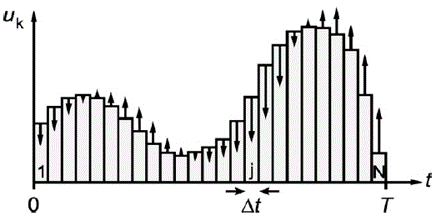
\includegraphics[width=0.7\columnwidth]{gfx/const_piece.png} % TODO: Change the image
    \caption{Example of a step-wise constant function as an array of numbers}
    \label{fig:step-wise-const}
\end{figure}
\section{The Cost Function}
When our desired operation is to prepare our quantum system in a predetermined state, a good figure of merit of how close our system is to the desired state is given by the \textbf{fidelity}. The fidelity is a measure of the "closeness" of two quantum states, The fidelity is $0$ when the two states are orthogonal, and $1$ if they are identical. The fidelity is given by the magnitude of the \textit{overlap} between the two states squared\footnote{Assuming both states are pure states and not mixed states}.

\begin{equation} \label{def:fid}
\mathcal{F} (\psi_1, \psi_2) = \abs{\braket{\psi_1}{\psi_2}}^2
\end{equation}
The \textit{infidelity}, $1 - \mathcal{F}$ between the two states, can be conveniently used as the cost function in our optimization procedure\footnote{Since we want to maximize the fidelity, we want to minimize the infidelity}. Given an initial state and a target state, along with the Hamiltonian and pulse information, we want to be able to calculate the fidelity for any given pulse. To do so, we need to solve Schr\"{o}dinger's equation for the pulse
\begin{equation}
i\hslash\frac{d}{dt}\ket{\Psi (t)} = \hat{\mathcal{H}}\ket{\Psi (t)}
\end{equation}
In the previous chapter we characterized the Hamiltonian of the system (equations (\ref{eq:JC-hamiltonian}) and (\ref{eq:dispersive-hamiltonian})),
% TODO: Add explanation about that there are multiple different pulses and throughout the chapter we're referring to a single pulse which is most of the time not the case
\begin{equation} \label{eq:hamiltonianl_form}
\hat{\mathcal{H}} (t) = \hat{\mathcal{H}}_0 + \sum_k{\epsilon_k (t) \hat{\mathcal{H}}_k} % Maybe put the next part before the part about the Schrodinger equation
\end{equation}
where $H_0$ is the (time-independent) Hamiltonian of the system without the drives (given, for example, from the Jaynes-Cummings model). Each $\epsilon_k (t)$ is the amplitude as a function of time of the control drive pulses, and each $H_k$ is the (time-independent)Hamiltonian describing the interaction between the control pulse and the rest of the system. We call these Hamiltonians the \textit{drive hamiltonians}. Our goal with GRAPE is to find optimal $\epsilon_k (t)$.

On each constant step of the amplitude functions $\epsilon_k (t)$, the entire Hamiltonian is constant. Luckily, the solution of the Schr\"{o}dinger equation for a constant Hamiltonian is easily solved by
\begin{equation}
\hat{U} (t) = e^{-\frac{i}{\hslash}\int_{T_0}^{T_1}\hat{\mathcal{H}} (t)dt}
\end{equation}
If we choose $T_0$ and $T_1$ as the end points of a step of the Hamiltonian, the total Hamiltonian of the system is constant so the integral is just a simple multiplication by $T_1-T_0$ which we'll write as $\delta t = T_1 - T_0$. The solution becomes
\begin{equation}
\hat{U} (t) = e^{-\frac{i\cdot \delta t}{\hslash}\hat{\mathcal{H}} (t)}
\end{equation}

In order to calculate the solution over the entire pulse we need to solve for the first step, then find the solution by the end of that time-step, and use it as the initial condition for the next time step, repeating for each time step. The solution until the $N^{th}$ time step is simply the product of the previous solutions for each time step
\begin{equation}\label{eq:U_def_prod}
\hat{U}_N (\epsilon (t)) = \prod_{k = 1}^N\hat{U}_k (\epsilon (t))
\end{equation}
With $\hat{U} (\epsilon)$ in hand, we can calculate the evolution of the state over the entire pulse
\begin{equation}
\ket{\Psi_{final}} = \hat{U} (\epsilon)\ket{\Psi_{initial}}
\end{equation}
This way, if we want to calculate the fidelity after applying the drives, we can simply calculate the fidelity between the target state and the final, calculated state
\begin{equation} \label{eq:fidelity_sim}
\mathcal{F} (\epsilon (t)) = \mathcal{F} (\Psi_{target}, \Psi_{final}) = \abs{\bra{\Psi_{target}}\hat{U}_N\ket{\Psi_{initial}}}^2
\end{equation}

As mentioned, if we want to optimize the cost function efficiently we'll need to calculate the gradient of the cost function along with the cost function itself.

\section{The Gradient}
For simplicity, we'll first derive the gradient of the \textit{overlap}
\begin{equation} \label{def:overlap}
c = \braket{\Psi_{target}}{\Psi_{final}} = \bra{\Psi_{target}}\hat{U}\ket{\Psi_{initial}}
\end{equation}
We can then get the fidelity by noting that $\mathcal{F} = \abs{c}^2$. We want to differentiate the overlap by each control parameter. To do so, note that $\hat{U}$ is defined as:
\[ 
\hat{U} = \hat{U}_N \hat{U}_{n-1}...\hat{U}_2 \hat{U}_1
\]
And when differentiating by a control parameter only one $\hat{U}_k$ is affected,
\[
\frac{\partial c}{\partial \epsilon_k} = \bra{\Psi_{target}}\hat{U}_N \hat{U}_{N-1} ... \hat{U}_{k+1}\frac{\partial \hat{U}}{\partial \epsilon_k} \hat{U}_{k-1} ...\hat{U}_2 \hat{U}_1\ket{\Psi_{initial}} 
\]
We can write that for a constant Hamiltonian (from Schr\"{o}dinger's equation)
\[
    \hat{U}_k = e^{-\frac{i\cdot \delta t}{\hslash}\hat{\mathcal{H}} (t)}
\]
And approximate the derivative $\frac{\partial \hat{U}_k}{\partial \epsilon_k}$ in the limit of small $\delta t$ by writing
\begin{equation*}
    \frac{\partial \hat{U}_k}{\partial \epsilon_k} \approx -\frac{i\cdot \delta t}{\hslash}\frac{\partial H}{\partial \epsilon_k} \cdot e^{-\frac{i\cdot \delta t}{\hslash}\hat{\mathcal{H}} (t)} = -\frac{i\cdot \delta t}{\hslash}\frac{\partial H}{\partial \epsilon_k} \hat{U}_k
\end{equation*}

Theoretically, we have everything we need to calculate the gradient, but it's still rather complex computationally ($o (N^2)$ complexity). A different method can be used to reduce the computational overhead.

The derivative of the cost function by a control parameter of the pulse has become
\begin{equation} \label{eq:cost_init_deriv}
    \frac{dc}{d\epsilon_k} = -\frac{i\cdot \delta t}{\hslash} \underbrace{\bra{\Psi_{target}}\hat{U}_N \hat{U}_{N-1}... \hat{U}_{k+1}}_{\bra{\psi_{bwd}^{ (k+1)}}}\frac{dH}{d\epsilon_k} \underbrace{\hat{U}_{k} ...\hat{U}_2 \hat{U}_1\ket{\Psi_{initial}}}_{\ket{\psi_{fwd}^{ (k)}}}
\end{equation}
Where we defined two arrays, $\bra{\psi_{bwd}}$ and $\ket{\psi_{fwd}}$, the multiplication components before and after the derivative of H
\begin{equation} \label{eq:cost-function-b/fwd}
    \frac{\partial c}{\partial \epsilon_k} =  -\frac{i\cdot \delta t}{\hslash}\bra{\psi_{bwd}^{ (k+1)}} \frac{\partial H}{\partial \epsilon_k} \ket{\psi_{fwd}^{ (k)}}
\end{equation}
We can see from \ref{eq:cost_init_deriv} that 
\[   
\ket{\psi_{fwd}^{ (k)}} = 
     \begin{cases}
       \ket{\psi_{init}} &\quad\ k=0\\
       \hat{U}_k \ket{\psi_{fwd}^{ (k-1)}} &\quad\ otherwise\\
     \end{cases}
\]
\[   
\ket{\psi_{bwd}^{ (k)}} = 
     \begin{cases}
       \ket{\psi_{targ}} &\quad\ k=N+1\\
       \hat{U}_k^{\dag{}} \ket{\psi_{bwd}^{ (k+1)}} &\quad\ otherwise\\
     \end{cases}
\]
Now all we need is to do $2N$ calculations in the beginning ($N$ for $bwd$ and $N$ for $fwd$), and then calculating the actual gradient using equation \ref{eq:cost-function-b/fwd}. This improves the computation complexity from $o (N^2)$ to $o (N)$, while the memory complexity stays $o (N)$.

It's important to note that $c$ is not the fidelity, but the overlap. We can get the fidelity from $c$ by
\[
\mathcal{F} = |c|^2
\]
since $c$ might be complex this derivative is a bit less trivial than it might seem. We can write $c (\vec{\epsilon})$ as $a (\vec{\epsilon}) + b (\vec{\epsilon})i$, where $a, b \in R$ and we get that 
\[
\frac{\partial \mathcal{F}}{\partial \epsilon_k} = \frac{\partial |c|^2}{\partial \epsilon_k} = \frac{\partial |a+bi|^2}{\partial \epsilon_k} = \frac{\partial (a^2 + b^2)}{\partial \epsilon_k} = 2 (a\frac{\partial a}{\partial \epsilon_k} + b\frac{\partial b}{\partial \epsilon_k})
\]
We can notice that $c (\frac{\partial c}{\partial \epsilon_k})^* = a\frac{\partial a}{\partial \epsilon_k} + b\frac{\partial b}{\partial \epsilon_k} + (ab - \frac{\partial a}{\partial \epsilon_k}\frac{\partial b}{\partial \epsilon_k})i$. More importantly, we can see that the real part of that expression is exactly what we need. Putting it all into one formula we get
\begin{equation} \label{eq:fidelity_gradient_final}
    \frac{\partial \mathcal{F}}{\partial \epsilon_k} = 2\cdot \Re{c (\frac{\partial c}{\partial \epsilon_k})^*}
\end{equation}
Now all you need is to plug \ref{eq:cost-function-b/fwd} and \ref{def:overlap} into \ref{eq:fidelity_gradient_final} and you got your gradient :)

Let's do a little test now to see that everything is working well. The simplest pulse you can send is the pulse that takes the qubit from being in state $\ket{0}$ to state $\ket{1}$, where the transition frequency is set to $1$Ghz (hence the period is $1$ns). We discussed this situation in appendix \ref{appen:annalytic} so we know how the solution should look like. Running our GRAPE code with some random initial pulse we get
% \begin{figure}[H]
%     \centering
%     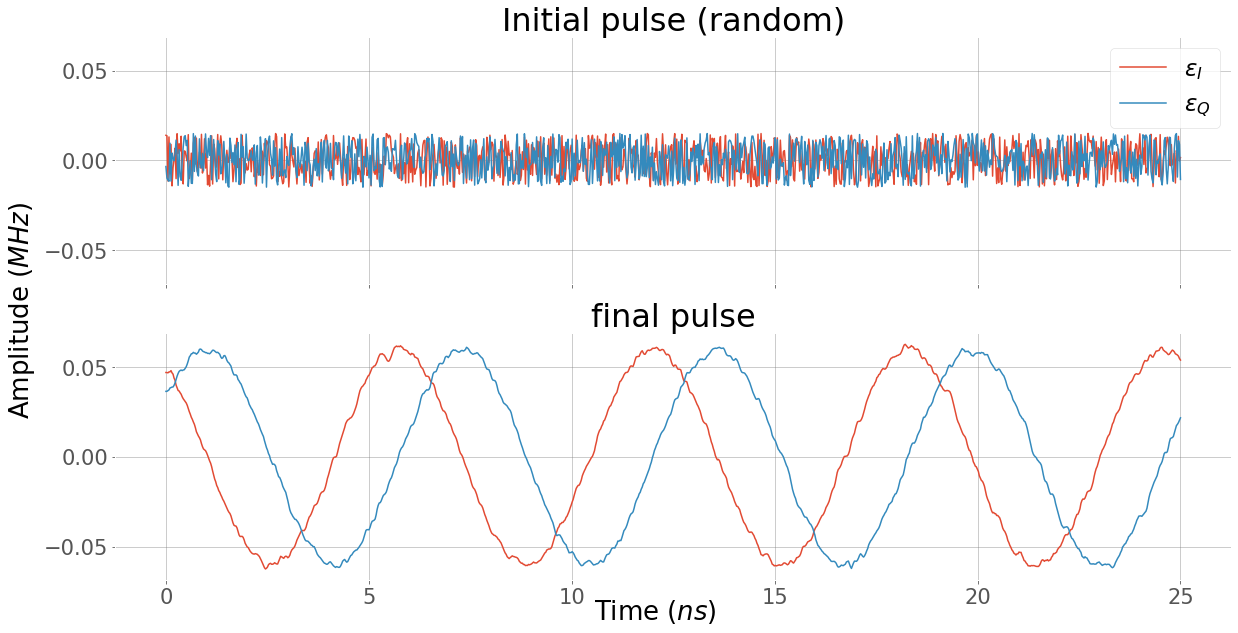
\includegraphics[width=1\columnwidth]{Results/No-Constraints-single-qubit/pulses-hella-prettier.png}
%     \caption{Pulses solution for $\ket{0} \rightarrow \ket{1}$. Each color is a different microwave control pulse of the system, I and Q. They are the real and imaginary parts of the calculated wave in appendix \ref{appen:annalytic} }
%     \label{fig:GRAPE-first-example}
% \end{figure}
\begin{figure}[H]
    \begin{center}
        %% Creator: Matplotlib, PGF backend
%%
%% To include the figure in your LaTeX document, write
%%   \input{<filename>.pgf}
%%
%% Make sure the required packages are loaded in your preamble
%%   \usepackage{pgf}
%%
%% and, on pdftex
%%   \usepackage[utf8]{inputenc}\DeclareUnicodeCharacter{2212}{-}
%%
%% or, on luatex and xetex
%%   \usepackage{unicode-math}
%%
%% Figures using additional raster images can only be included by \input if
%% they are in the same directory as the main LaTeX file. For loading figures
%% from other directories you can use the `import` package
%%   \usepackage{import}
%%
%% and then include the figures with
%%   \import{<path to file>}{<filename>.pgf}
%%
%% Matplotlib used the following preamble
%%
\begingroup%
\makeatletter%
\begin{pgfpicture}%
\pgfpathrectangle{\pgfpointorigin}{\pgfqpoint{4.650000in}{2.300000in}}%
\pgfusepath{use as bounding box, clip}%
\begin{pgfscope}%
\pgfsetbuttcap%
\pgfsetmiterjoin%
\definecolor{currentfill}{rgb}{1.000000,1.000000,1.000000}%
\pgfsetfillcolor{currentfill}%
\pgfsetlinewidth{0.000000pt}%
\definecolor{currentstroke}{rgb}{1.000000,1.000000,1.000000}%
\pgfsetstrokecolor{currentstroke}%
\pgfsetdash{}{0pt}%
\pgfpathmoveto{\pgfqpoint{0.000000in}{0.000000in}}%
\pgfpathlineto{\pgfqpoint{4.650000in}{0.000000in}}%
\pgfpathlineto{\pgfqpoint{4.650000in}{2.300000in}}%
\pgfpathlineto{\pgfqpoint{0.000000in}{2.300000in}}%
\pgfpathclose%
\pgfusepath{fill}%
\end{pgfscope}%
\begin{pgfscope}%
\pgfsetbuttcap%
\pgfsetmiterjoin%
\definecolor{currentfill}{rgb}{1.000000,1.000000,1.000000}%
\pgfsetfillcolor{currentfill}%
\pgfsetlinewidth{0.000000pt}%
\definecolor{currentstroke}{rgb}{0.000000,0.000000,0.000000}%
\pgfsetstrokecolor{currentstroke}%
\pgfsetstrokeopacity{0.000000}%
\pgfsetdash{}{0pt}%
\pgfpathmoveto{\pgfqpoint{0.602162in}{1.354089in}}%
\pgfpathlineto{\pgfqpoint{4.500000in}{1.354089in}}%
\pgfpathlineto{\pgfqpoint{4.500000in}{1.916667in}}%
\pgfpathlineto{\pgfqpoint{0.602162in}{1.916667in}}%
\pgfpathclose%
\pgfusepath{fill}%
\end{pgfscope}%
\begin{pgfscope}%
\pgfpathrectangle{\pgfqpoint{0.602162in}{1.354089in}}{\pgfqpoint{3.897838in}{0.562577in}}%
\pgfusepath{clip}%
\pgfsetrectcap%
\pgfsetroundjoin%
\pgfsetlinewidth{0.803000pt}%
\definecolor{currentstroke}{rgb}{0.501961,0.501961,0.501961}%
\pgfsetstrokecolor{currentstroke}%
\pgfsetstrokeopacity{0.200000}%
\pgfsetdash{}{0pt}%
\pgfpathmoveto{\pgfqpoint{0.779336in}{1.354089in}}%
\pgfpathlineto{\pgfqpoint{0.779336in}{1.916667in}}%
\pgfusepath{stroke}%
\end{pgfscope}%
\begin{pgfscope}%
\pgfsetbuttcap%
\pgfsetroundjoin%
\definecolor{currentfill}{rgb}{0.333333,0.333333,0.333333}%
\pgfsetfillcolor{currentfill}%
\pgfsetlinewidth{0.803000pt}%
\definecolor{currentstroke}{rgb}{0.333333,0.333333,0.333333}%
\pgfsetstrokecolor{currentstroke}%
\pgfsetdash{}{0pt}%
\pgfsys@defobject{currentmarker}{\pgfqpoint{0.000000in}{-0.048611in}}{\pgfqpoint{0.000000in}{0.000000in}}{%
\pgfpathmoveto{\pgfqpoint{0.000000in}{0.000000in}}%
\pgfpathlineto{\pgfqpoint{0.000000in}{-0.048611in}}%
\pgfusepath{stroke,fill}%
}%
\begin{pgfscope}%
\pgfsys@transformshift{0.779336in}{1.354089in}%
\pgfsys@useobject{currentmarker}{}%
\end{pgfscope}%
\end{pgfscope}%
\begin{pgfscope}%
\pgfpathrectangle{\pgfqpoint{0.602162in}{1.354089in}}{\pgfqpoint{3.897838in}{0.562577in}}%
\pgfusepath{clip}%
\pgfsetrectcap%
\pgfsetroundjoin%
\pgfsetlinewidth{0.803000pt}%
\definecolor{currentstroke}{rgb}{0.501961,0.501961,0.501961}%
\pgfsetstrokecolor{currentstroke}%
\pgfsetstrokeopacity{0.200000}%
\pgfsetdash{}{0pt}%
\pgfpathmoveto{\pgfqpoint{1.488034in}{1.354089in}}%
\pgfpathlineto{\pgfqpoint{1.488034in}{1.916667in}}%
\pgfusepath{stroke}%
\end{pgfscope}%
\begin{pgfscope}%
\pgfsetbuttcap%
\pgfsetroundjoin%
\definecolor{currentfill}{rgb}{0.333333,0.333333,0.333333}%
\pgfsetfillcolor{currentfill}%
\pgfsetlinewidth{0.803000pt}%
\definecolor{currentstroke}{rgb}{0.333333,0.333333,0.333333}%
\pgfsetstrokecolor{currentstroke}%
\pgfsetdash{}{0pt}%
\pgfsys@defobject{currentmarker}{\pgfqpoint{0.000000in}{-0.048611in}}{\pgfqpoint{0.000000in}{0.000000in}}{%
\pgfpathmoveto{\pgfqpoint{0.000000in}{0.000000in}}%
\pgfpathlineto{\pgfqpoint{0.000000in}{-0.048611in}}%
\pgfusepath{stroke,fill}%
}%
\begin{pgfscope}%
\pgfsys@transformshift{1.488034in}{1.354089in}%
\pgfsys@useobject{currentmarker}{}%
\end{pgfscope}%
\end{pgfscope}%
\begin{pgfscope}%
\pgfpathrectangle{\pgfqpoint{0.602162in}{1.354089in}}{\pgfqpoint{3.897838in}{0.562577in}}%
\pgfusepath{clip}%
\pgfsetrectcap%
\pgfsetroundjoin%
\pgfsetlinewidth{0.803000pt}%
\definecolor{currentstroke}{rgb}{0.501961,0.501961,0.501961}%
\pgfsetstrokecolor{currentstroke}%
\pgfsetstrokeopacity{0.200000}%
\pgfsetdash{}{0pt}%
\pgfpathmoveto{\pgfqpoint{2.196732in}{1.354089in}}%
\pgfpathlineto{\pgfqpoint{2.196732in}{1.916667in}}%
\pgfusepath{stroke}%
\end{pgfscope}%
\begin{pgfscope}%
\pgfsetbuttcap%
\pgfsetroundjoin%
\definecolor{currentfill}{rgb}{0.333333,0.333333,0.333333}%
\pgfsetfillcolor{currentfill}%
\pgfsetlinewidth{0.803000pt}%
\definecolor{currentstroke}{rgb}{0.333333,0.333333,0.333333}%
\pgfsetstrokecolor{currentstroke}%
\pgfsetdash{}{0pt}%
\pgfsys@defobject{currentmarker}{\pgfqpoint{0.000000in}{-0.048611in}}{\pgfqpoint{0.000000in}{0.000000in}}{%
\pgfpathmoveto{\pgfqpoint{0.000000in}{0.000000in}}%
\pgfpathlineto{\pgfqpoint{0.000000in}{-0.048611in}}%
\pgfusepath{stroke,fill}%
}%
\begin{pgfscope}%
\pgfsys@transformshift{2.196732in}{1.354089in}%
\pgfsys@useobject{currentmarker}{}%
\end{pgfscope}%
\end{pgfscope}%
\begin{pgfscope}%
\pgfpathrectangle{\pgfqpoint{0.602162in}{1.354089in}}{\pgfqpoint{3.897838in}{0.562577in}}%
\pgfusepath{clip}%
\pgfsetrectcap%
\pgfsetroundjoin%
\pgfsetlinewidth{0.803000pt}%
\definecolor{currentstroke}{rgb}{0.501961,0.501961,0.501961}%
\pgfsetstrokecolor{currentstroke}%
\pgfsetstrokeopacity{0.200000}%
\pgfsetdash{}{0pt}%
\pgfpathmoveto{\pgfqpoint{2.905430in}{1.354089in}}%
\pgfpathlineto{\pgfqpoint{2.905430in}{1.916667in}}%
\pgfusepath{stroke}%
\end{pgfscope}%
\begin{pgfscope}%
\pgfsetbuttcap%
\pgfsetroundjoin%
\definecolor{currentfill}{rgb}{0.333333,0.333333,0.333333}%
\pgfsetfillcolor{currentfill}%
\pgfsetlinewidth{0.803000pt}%
\definecolor{currentstroke}{rgb}{0.333333,0.333333,0.333333}%
\pgfsetstrokecolor{currentstroke}%
\pgfsetdash{}{0pt}%
\pgfsys@defobject{currentmarker}{\pgfqpoint{0.000000in}{-0.048611in}}{\pgfqpoint{0.000000in}{0.000000in}}{%
\pgfpathmoveto{\pgfqpoint{0.000000in}{0.000000in}}%
\pgfpathlineto{\pgfqpoint{0.000000in}{-0.048611in}}%
\pgfusepath{stroke,fill}%
}%
\begin{pgfscope}%
\pgfsys@transformshift{2.905430in}{1.354089in}%
\pgfsys@useobject{currentmarker}{}%
\end{pgfscope}%
\end{pgfscope}%
\begin{pgfscope}%
\pgfpathrectangle{\pgfqpoint{0.602162in}{1.354089in}}{\pgfqpoint{3.897838in}{0.562577in}}%
\pgfusepath{clip}%
\pgfsetrectcap%
\pgfsetroundjoin%
\pgfsetlinewidth{0.803000pt}%
\definecolor{currentstroke}{rgb}{0.501961,0.501961,0.501961}%
\pgfsetstrokecolor{currentstroke}%
\pgfsetstrokeopacity{0.200000}%
\pgfsetdash{}{0pt}%
\pgfpathmoveto{\pgfqpoint{3.614128in}{1.354089in}}%
\pgfpathlineto{\pgfqpoint{3.614128in}{1.916667in}}%
\pgfusepath{stroke}%
\end{pgfscope}%
\begin{pgfscope}%
\pgfsetbuttcap%
\pgfsetroundjoin%
\definecolor{currentfill}{rgb}{0.333333,0.333333,0.333333}%
\pgfsetfillcolor{currentfill}%
\pgfsetlinewidth{0.803000pt}%
\definecolor{currentstroke}{rgb}{0.333333,0.333333,0.333333}%
\pgfsetstrokecolor{currentstroke}%
\pgfsetdash{}{0pt}%
\pgfsys@defobject{currentmarker}{\pgfqpoint{0.000000in}{-0.048611in}}{\pgfqpoint{0.000000in}{0.000000in}}{%
\pgfpathmoveto{\pgfqpoint{0.000000in}{0.000000in}}%
\pgfpathlineto{\pgfqpoint{0.000000in}{-0.048611in}}%
\pgfusepath{stroke,fill}%
}%
\begin{pgfscope}%
\pgfsys@transformshift{3.614128in}{1.354089in}%
\pgfsys@useobject{currentmarker}{}%
\end{pgfscope}%
\end{pgfscope}%
\begin{pgfscope}%
\pgfpathrectangle{\pgfqpoint{0.602162in}{1.354089in}}{\pgfqpoint{3.897838in}{0.562577in}}%
\pgfusepath{clip}%
\pgfsetrectcap%
\pgfsetroundjoin%
\pgfsetlinewidth{0.803000pt}%
\definecolor{currentstroke}{rgb}{0.501961,0.501961,0.501961}%
\pgfsetstrokecolor{currentstroke}%
\pgfsetstrokeopacity{0.200000}%
\pgfsetdash{}{0pt}%
\pgfpathmoveto{\pgfqpoint{4.322826in}{1.354089in}}%
\pgfpathlineto{\pgfqpoint{4.322826in}{1.916667in}}%
\pgfusepath{stroke}%
\end{pgfscope}%
\begin{pgfscope}%
\pgfsetbuttcap%
\pgfsetroundjoin%
\definecolor{currentfill}{rgb}{0.333333,0.333333,0.333333}%
\pgfsetfillcolor{currentfill}%
\pgfsetlinewidth{0.803000pt}%
\definecolor{currentstroke}{rgb}{0.333333,0.333333,0.333333}%
\pgfsetstrokecolor{currentstroke}%
\pgfsetdash{}{0pt}%
\pgfsys@defobject{currentmarker}{\pgfqpoint{0.000000in}{-0.048611in}}{\pgfqpoint{0.000000in}{0.000000in}}{%
\pgfpathmoveto{\pgfqpoint{0.000000in}{0.000000in}}%
\pgfpathlineto{\pgfqpoint{0.000000in}{-0.048611in}}%
\pgfusepath{stroke,fill}%
}%
\begin{pgfscope}%
\pgfsys@transformshift{4.322826in}{1.354089in}%
\pgfsys@useobject{currentmarker}{}%
\end{pgfscope}%
\end{pgfscope}%
\begin{pgfscope}%
\pgfpathrectangle{\pgfqpoint{0.602162in}{1.354089in}}{\pgfqpoint{3.897838in}{0.562577in}}%
\pgfusepath{clip}%
\pgfsetrectcap%
\pgfsetroundjoin%
\pgfsetlinewidth{0.803000pt}%
\definecolor{currentstroke}{rgb}{0.501961,0.501961,0.501961}%
\pgfsetstrokecolor{currentstroke}%
\pgfsetstrokeopacity{0.200000}%
\pgfsetdash{}{0pt}%
\pgfpathmoveto{\pgfqpoint{0.602162in}{1.434660in}}%
\pgfpathlineto{\pgfqpoint{4.500000in}{1.434660in}}%
\pgfusepath{stroke}%
\end{pgfscope}%
\begin{pgfscope}%
\pgfsetbuttcap%
\pgfsetroundjoin%
\definecolor{currentfill}{rgb}{0.333333,0.333333,0.333333}%
\pgfsetfillcolor{currentfill}%
\pgfsetlinewidth{0.803000pt}%
\definecolor{currentstroke}{rgb}{0.333333,0.333333,0.333333}%
\pgfsetstrokecolor{currentstroke}%
\pgfsetdash{}{0pt}%
\pgfsys@defobject{currentmarker}{\pgfqpoint{-0.048611in}{0.000000in}}{\pgfqpoint{0.000000in}{0.000000in}}{%
\pgfpathmoveto{\pgfqpoint{0.000000in}{0.000000in}}%
\pgfpathlineto{\pgfqpoint{-0.048611in}{0.000000in}}%
\pgfusepath{stroke,fill}%
}%
\begin{pgfscope}%
\pgfsys@transformshift{0.602162in}{1.434660in}%
\pgfsys@useobject{currentmarker}{}%
\end{pgfscope}%
\end{pgfscope}%
\begin{pgfscope}%
\definecolor{textcolor}{rgb}{0.333333,0.333333,0.333333}%
\pgfsetstrokecolor{textcolor}%
\pgfsetfillcolor{textcolor}%
\pgftext[x=0.150000in, y=1.386435in, left, base]{\color{textcolor}\rmfamily\fontsize{10.000000}{12.000000}\selectfont \(\displaystyle {-0.05}\)}%
\end{pgfscope}%
\begin{pgfscope}%
\pgfpathrectangle{\pgfqpoint{0.602162in}{1.354089in}}{\pgfqpoint{3.897838in}{0.562577in}}%
\pgfusepath{clip}%
\pgfsetrectcap%
\pgfsetroundjoin%
\pgfsetlinewidth{0.803000pt}%
\definecolor{currentstroke}{rgb}{0.501961,0.501961,0.501961}%
\pgfsetstrokecolor{currentstroke}%
\pgfsetstrokeopacity{0.200000}%
\pgfsetdash{}{0pt}%
\pgfpathmoveto{\pgfqpoint{0.602162in}{1.633153in}}%
\pgfpathlineto{\pgfqpoint{4.500000in}{1.633153in}}%
\pgfusepath{stroke}%
\end{pgfscope}%
\begin{pgfscope}%
\pgfsetbuttcap%
\pgfsetroundjoin%
\definecolor{currentfill}{rgb}{0.333333,0.333333,0.333333}%
\pgfsetfillcolor{currentfill}%
\pgfsetlinewidth{0.803000pt}%
\definecolor{currentstroke}{rgb}{0.333333,0.333333,0.333333}%
\pgfsetstrokecolor{currentstroke}%
\pgfsetdash{}{0pt}%
\pgfsys@defobject{currentmarker}{\pgfqpoint{-0.048611in}{0.000000in}}{\pgfqpoint{0.000000in}{0.000000in}}{%
\pgfpathmoveto{\pgfqpoint{0.000000in}{0.000000in}}%
\pgfpathlineto{\pgfqpoint{-0.048611in}{0.000000in}}%
\pgfusepath{stroke,fill}%
}%
\begin{pgfscope}%
\pgfsys@transformshift{0.602162in}{1.633153in}%
\pgfsys@useobject{currentmarker}{}%
\end{pgfscope}%
\end{pgfscope}%
\begin{pgfscope}%
\definecolor{textcolor}{rgb}{0.333333,0.333333,0.333333}%
\pgfsetstrokecolor{textcolor}%
\pgfsetfillcolor{textcolor}%
\pgftext[x=0.258025in, y=1.584928in, left, base]{\color{textcolor}\rmfamily\fontsize{10.000000}{12.000000}\selectfont \(\displaystyle {0.00}\)}%
\end{pgfscope}%
\begin{pgfscope}%
\pgfpathrectangle{\pgfqpoint{0.602162in}{1.354089in}}{\pgfqpoint{3.897838in}{0.562577in}}%
\pgfusepath{clip}%
\pgfsetrectcap%
\pgfsetroundjoin%
\pgfsetlinewidth{0.803000pt}%
\definecolor{currentstroke}{rgb}{0.501961,0.501961,0.501961}%
\pgfsetstrokecolor{currentstroke}%
\pgfsetstrokeopacity{0.200000}%
\pgfsetdash{}{0pt}%
\pgfpathmoveto{\pgfqpoint{0.602162in}{1.831646in}}%
\pgfpathlineto{\pgfqpoint{4.500000in}{1.831646in}}%
\pgfusepath{stroke}%
\end{pgfscope}%
\begin{pgfscope}%
\pgfsetbuttcap%
\pgfsetroundjoin%
\definecolor{currentfill}{rgb}{0.333333,0.333333,0.333333}%
\pgfsetfillcolor{currentfill}%
\pgfsetlinewidth{0.803000pt}%
\definecolor{currentstroke}{rgb}{0.333333,0.333333,0.333333}%
\pgfsetstrokecolor{currentstroke}%
\pgfsetdash{}{0pt}%
\pgfsys@defobject{currentmarker}{\pgfqpoint{-0.048611in}{0.000000in}}{\pgfqpoint{0.000000in}{0.000000in}}{%
\pgfpathmoveto{\pgfqpoint{0.000000in}{0.000000in}}%
\pgfpathlineto{\pgfqpoint{-0.048611in}{0.000000in}}%
\pgfusepath{stroke,fill}%
}%
\begin{pgfscope}%
\pgfsys@transformshift{0.602162in}{1.831646in}%
\pgfsys@useobject{currentmarker}{}%
\end{pgfscope}%
\end{pgfscope}%
\begin{pgfscope}%
\definecolor{textcolor}{rgb}{0.333333,0.333333,0.333333}%
\pgfsetstrokecolor{textcolor}%
\pgfsetfillcolor{textcolor}%
\pgftext[x=0.258025in, y=1.783421in, left, base]{\color{textcolor}\rmfamily\fontsize{10.000000}{12.000000}\selectfont \(\displaystyle {0.05}\)}%
\end{pgfscope}%
\begin{pgfscope}%
\pgfpathrectangle{\pgfqpoint{0.602162in}{1.354089in}}{\pgfqpoint{3.897838in}{0.562577in}}%
\pgfusepath{clip}%
\pgfsetrectcap%
\pgfsetroundjoin%
\pgfsetlinewidth{1.505625pt}%
\definecolor{currentstroke}{rgb}{0.886275,0.290196,0.200000}%
\pgfsetstrokecolor{currentstroke}%
\pgfsetdash{}{0pt}%
\pgfpathmoveto{\pgfqpoint{0.779336in}{1.614964in}}%
\pgfpathlineto{\pgfqpoint{0.815129in}{1.631586in}}%
\pgfpathlineto{\pgfqpoint{0.850922in}{1.619567in}}%
\pgfpathlineto{\pgfqpoint{0.886714in}{1.650574in}}%
\pgfpathlineto{\pgfqpoint{0.922507in}{1.619848in}}%
\pgfpathlineto{\pgfqpoint{0.958300in}{1.613819in}}%
\pgfpathlineto{\pgfqpoint{0.994093in}{1.636543in}}%
\pgfpathlineto{\pgfqpoint{1.029886in}{1.636064in}}%
\pgfpathlineto{\pgfqpoint{1.065679in}{1.625355in}}%
\pgfpathlineto{\pgfqpoint{1.101471in}{1.620960in}}%
\pgfpathlineto{\pgfqpoint{1.137264in}{1.652967in}}%
\pgfpathlineto{\pgfqpoint{1.173057in}{1.645826in}}%
\pgfpathlineto{\pgfqpoint{1.208850in}{1.617558in}}%
\pgfpathlineto{\pgfqpoint{1.244643in}{1.631170in}}%
\pgfpathlineto{\pgfqpoint{1.280436in}{1.650506in}}%
\pgfpathlineto{\pgfqpoint{1.316228in}{1.619952in}}%
\pgfpathlineto{\pgfqpoint{1.352021in}{1.636022in}}%
\pgfpathlineto{\pgfqpoint{1.387814in}{1.647308in}}%
\pgfpathlineto{\pgfqpoint{1.423607in}{1.650700in}}%
\pgfpathlineto{\pgfqpoint{1.459400in}{1.632414in}}%
\pgfpathlineto{\pgfqpoint{1.495192in}{1.636649in}}%
\pgfpathlineto{\pgfqpoint{1.530985in}{1.637150in}}%
\pgfpathlineto{\pgfqpoint{1.566778in}{1.649395in}}%
\pgfpathlineto{\pgfqpoint{1.602571in}{1.616914in}}%
\pgfpathlineto{\pgfqpoint{1.638364in}{1.619419in}}%
\pgfpathlineto{\pgfqpoint{1.674157in}{1.649919in}}%
\pgfpathlineto{\pgfqpoint{1.709949in}{1.624610in}}%
\pgfpathlineto{\pgfqpoint{1.745742in}{1.618789in}}%
\pgfpathlineto{\pgfqpoint{1.781535in}{1.627908in}}%
\pgfpathlineto{\pgfqpoint{1.817328in}{1.623307in}}%
\pgfpathlineto{\pgfqpoint{1.853121in}{1.620499in}}%
\pgfpathlineto{\pgfqpoint{1.888914in}{1.642843in}}%
\pgfpathlineto{\pgfqpoint{1.924706in}{1.645126in}}%
\pgfpathlineto{\pgfqpoint{1.960499in}{1.628178in}}%
\pgfpathlineto{\pgfqpoint{1.996292in}{1.626547in}}%
\pgfpathlineto{\pgfqpoint{2.032085in}{1.640373in}}%
\pgfpathlineto{\pgfqpoint{2.067878in}{1.626959in}}%
\pgfpathlineto{\pgfqpoint{2.103670in}{1.637159in}}%
\pgfpathlineto{\pgfqpoint{2.139463in}{1.643447in}}%
\pgfpathlineto{\pgfqpoint{2.175256in}{1.636876in}}%
\pgfpathlineto{\pgfqpoint{2.211049in}{1.643328in}}%
\pgfpathlineto{\pgfqpoint{2.246842in}{1.615698in}}%
\pgfpathlineto{\pgfqpoint{2.282635in}{1.642543in}}%
\pgfpathlineto{\pgfqpoint{2.318427in}{1.640004in}}%
\pgfpathlineto{\pgfqpoint{2.354220in}{1.650906in}}%
\pgfpathlineto{\pgfqpoint{2.390013in}{1.615860in}}%
\pgfpathlineto{\pgfqpoint{2.425806in}{1.616127in}}%
\pgfpathlineto{\pgfqpoint{2.461599in}{1.639848in}}%
\pgfpathlineto{\pgfqpoint{2.497392in}{1.642084in}}%
\pgfpathlineto{\pgfqpoint{2.533184in}{1.631287in}}%
\pgfpathlineto{\pgfqpoint{2.568977in}{1.648372in}}%
\pgfpathlineto{\pgfqpoint{2.604770in}{1.623873in}}%
\pgfpathlineto{\pgfqpoint{2.640563in}{1.614653in}}%
\pgfpathlineto{\pgfqpoint{2.676356in}{1.625535in}}%
\pgfpathlineto{\pgfqpoint{2.712148in}{1.621462in}}%
\pgfpathlineto{\pgfqpoint{2.747941in}{1.640211in}}%
\pgfpathlineto{\pgfqpoint{2.783734in}{1.635742in}}%
\pgfpathlineto{\pgfqpoint{2.819527in}{1.646014in}}%
\pgfpathlineto{\pgfqpoint{2.855320in}{1.626906in}}%
\pgfpathlineto{\pgfqpoint{2.891113in}{1.643789in}}%
\pgfpathlineto{\pgfqpoint{2.926905in}{1.651105in}}%
\pgfpathlineto{\pgfqpoint{2.962698in}{1.625834in}}%
\pgfpathlineto{\pgfqpoint{2.998491in}{1.620377in}}%
\pgfpathlineto{\pgfqpoint{3.034284in}{1.625319in}}%
\pgfpathlineto{\pgfqpoint{3.070077in}{1.615970in}}%
\pgfpathlineto{\pgfqpoint{3.105870in}{1.621284in}}%
\pgfpathlineto{\pgfqpoint{3.141662in}{1.636090in}}%
\pgfpathlineto{\pgfqpoint{3.177455in}{1.633809in}}%
\pgfpathlineto{\pgfqpoint{3.213248in}{1.618403in}}%
\pgfpathlineto{\pgfqpoint{3.249041in}{1.646575in}}%
\pgfpathlineto{\pgfqpoint{3.284834in}{1.643659in}}%
\pgfpathlineto{\pgfqpoint{3.320626in}{1.615354in}}%
\pgfpathlineto{\pgfqpoint{3.356419in}{1.645952in}}%
\pgfpathlineto{\pgfqpoint{3.392212in}{1.644840in}}%
\pgfpathlineto{\pgfqpoint{3.428005in}{1.620415in}}%
\pgfpathlineto{\pgfqpoint{3.463798in}{1.638113in}}%
\pgfpathlineto{\pgfqpoint{3.499591in}{1.618064in}}%
\pgfpathlineto{\pgfqpoint{3.535383in}{1.614618in}}%
\pgfpathlineto{\pgfqpoint{3.571176in}{1.630775in}}%
\pgfpathlineto{\pgfqpoint{3.606969in}{1.617038in}}%
\pgfpathlineto{\pgfqpoint{3.642762in}{1.645108in}}%
\pgfpathlineto{\pgfqpoint{3.678555in}{1.624867in}}%
\pgfpathlineto{\pgfqpoint{3.714348in}{1.631724in}}%
\pgfpathlineto{\pgfqpoint{3.750140in}{1.631254in}}%
\pgfpathlineto{\pgfqpoint{3.785933in}{1.618379in}}%
\pgfpathlineto{\pgfqpoint{3.821726in}{1.627107in}}%
\pgfpathlineto{\pgfqpoint{3.857519in}{1.622912in}}%
\pgfpathlineto{\pgfqpoint{3.893312in}{1.641538in}}%
\pgfpathlineto{\pgfqpoint{3.929104in}{1.639527in}}%
\pgfpathlineto{\pgfqpoint{3.964897in}{1.645883in}}%
\pgfpathlineto{\pgfqpoint{4.000690in}{1.630953in}}%
\pgfpathlineto{\pgfqpoint{4.036483in}{1.616540in}}%
\pgfpathlineto{\pgfqpoint{4.072276in}{1.628818in}}%
\pgfpathlineto{\pgfqpoint{4.108069in}{1.636295in}}%
\pgfpathlineto{\pgfqpoint{4.143861in}{1.629833in}}%
\pgfpathlineto{\pgfqpoint{4.179654in}{1.641867in}}%
\pgfpathlineto{\pgfqpoint{4.215447in}{1.650241in}}%
\pgfpathlineto{\pgfqpoint{4.251240in}{1.632937in}}%
\pgfpathlineto{\pgfqpoint{4.287033in}{1.639743in}}%
\pgfpathlineto{\pgfqpoint{4.322826in}{1.627542in}}%
\pgfusepath{stroke}%
\end{pgfscope}%
\begin{pgfscope}%
\pgfpathrectangle{\pgfqpoint{0.602162in}{1.354089in}}{\pgfqpoint{3.897838in}{0.562577in}}%
\pgfusepath{clip}%
\pgfsetrectcap%
\pgfsetroundjoin%
\pgfsetlinewidth{1.505625pt}%
\definecolor{currentstroke}{rgb}{0.203922,0.541176,0.741176}%
\pgfsetstrokecolor{currentstroke}%
\pgfsetdash{}{0pt}%
\pgfpathmoveto{\pgfqpoint{0.779336in}{1.616572in}}%
\pgfpathlineto{\pgfqpoint{0.815129in}{1.617388in}}%
\pgfpathlineto{\pgfqpoint{0.850922in}{1.641192in}}%
\pgfpathlineto{\pgfqpoint{0.886714in}{1.622512in}}%
\pgfpathlineto{\pgfqpoint{0.922507in}{1.634388in}}%
\pgfpathlineto{\pgfqpoint{0.958300in}{1.622295in}}%
\pgfpathlineto{\pgfqpoint{0.994093in}{1.643926in}}%
\pgfpathlineto{\pgfqpoint{1.029886in}{1.630014in}}%
\pgfpathlineto{\pgfqpoint{1.065679in}{1.643738in}}%
\pgfpathlineto{\pgfqpoint{1.101471in}{1.652261in}}%
\pgfpathlineto{\pgfqpoint{1.137264in}{1.617461in}}%
\pgfpathlineto{\pgfqpoint{1.173057in}{1.631871in}}%
\pgfpathlineto{\pgfqpoint{1.208850in}{1.623124in}}%
\pgfpathlineto{\pgfqpoint{1.244643in}{1.620184in}}%
\pgfpathlineto{\pgfqpoint{1.280436in}{1.632746in}}%
\pgfpathlineto{\pgfqpoint{1.316228in}{1.614944in}}%
\pgfpathlineto{\pgfqpoint{1.352021in}{1.643509in}}%
\pgfpathlineto{\pgfqpoint{1.387814in}{1.632649in}}%
\pgfpathlineto{\pgfqpoint{1.423607in}{1.634863in}}%
\pgfpathlineto{\pgfqpoint{1.459400in}{1.624578in}}%
\pgfpathlineto{\pgfqpoint{1.495192in}{1.615662in}}%
\pgfpathlineto{\pgfqpoint{1.530985in}{1.616600in}}%
\pgfpathlineto{\pgfqpoint{1.566778in}{1.628587in}}%
\pgfpathlineto{\pgfqpoint{1.602571in}{1.644830in}}%
\pgfpathlineto{\pgfqpoint{1.638364in}{1.652391in}}%
\pgfpathlineto{\pgfqpoint{1.674157in}{1.641507in}}%
\pgfpathlineto{\pgfqpoint{1.709949in}{1.648625in}}%
\pgfpathlineto{\pgfqpoint{1.745742in}{1.651569in}}%
\pgfpathlineto{\pgfqpoint{1.781535in}{1.629365in}}%
\pgfpathlineto{\pgfqpoint{1.817328in}{1.625493in}}%
\pgfpathlineto{\pgfqpoint{1.853121in}{1.649149in}}%
\pgfpathlineto{\pgfqpoint{1.888914in}{1.647106in}}%
\pgfpathlineto{\pgfqpoint{1.924706in}{1.628936in}}%
\pgfpathlineto{\pgfqpoint{1.960499in}{1.634729in}}%
\pgfpathlineto{\pgfqpoint{1.996292in}{1.640869in}}%
\pgfpathlineto{\pgfqpoint{2.032085in}{1.637407in}}%
\pgfpathlineto{\pgfqpoint{2.067878in}{1.615601in}}%
\pgfpathlineto{\pgfqpoint{2.103670in}{1.637835in}}%
\pgfpathlineto{\pgfqpoint{2.139463in}{1.642009in}}%
\pgfpathlineto{\pgfqpoint{2.175256in}{1.642689in}}%
\pgfpathlineto{\pgfqpoint{2.211049in}{1.622810in}}%
\pgfpathlineto{\pgfqpoint{2.246842in}{1.624435in}}%
\pgfpathlineto{\pgfqpoint{2.282635in}{1.616232in}}%
\pgfpathlineto{\pgfqpoint{2.318427in}{1.630579in}}%
\pgfpathlineto{\pgfqpoint{2.354220in}{1.644659in}}%
\pgfpathlineto{\pgfqpoint{2.390013in}{1.630378in}}%
\pgfpathlineto{\pgfqpoint{2.425806in}{1.629494in}}%
\pgfpathlineto{\pgfqpoint{2.461599in}{1.621280in}}%
\pgfpathlineto{\pgfqpoint{2.497392in}{1.615464in}}%
\pgfpathlineto{\pgfqpoint{2.533184in}{1.614880in}}%
\pgfpathlineto{\pgfqpoint{2.568977in}{1.613744in}}%
\pgfpathlineto{\pgfqpoint{2.604770in}{1.617513in}}%
\pgfpathlineto{\pgfqpoint{2.640563in}{1.641966in}}%
\pgfpathlineto{\pgfqpoint{2.676356in}{1.639306in}}%
\pgfpathlineto{\pgfqpoint{2.712148in}{1.645798in}}%
\pgfpathlineto{\pgfqpoint{2.747941in}{1.642059in}}%
\pgfpathlineto{\pgfqpoint{2.783734in}{1.632903in}}%
\pgfpathlineto{\pgfqpoint{2.819527in}{1.638820in}}%
\pgfpathlineto{\pgfqpoint{2.855320in}{1.631711in}}%
\pgfpathlineto{\pgfqpoint{2.891113in}{1.643463in}}%
\pgfpathlineto{\pgfqpoint{2.926905in}{1.628166in}}%
\pgfpathlineto{\pgfqpoint{2.962698in}{1.634377in}}%
\pgfpathlineto{\pgfqpoint{2.998491in}{1.633543in}}%
\pgfpathlineto{\pgfqpoint{3.034284in}{1.632327in}}%
\pgfpathlineto{\pgfqpoint{3.070077in}{1.640843in}}%
\pgfpathlineto{\pgfqpoint{3.105870in}{1.628737in}}%
\pgfpathlineto{\pgfqpoint{3.141662in}{1.648972in}}%
\pgfpathlineto{\pgfqpoint{3.177455in}{1.638898in}}%
\pgfpathlineto{\pgfqpoint{3.213248in}{1.631223in}}%
\pgfpathlineto{\pgfqpoint{3.249041in}{1.650839in}}%
\pgfpathlineto{\pgfqpoint{3.284834in}{1.617456in}}%
\pgfpathlineto{\pgfqpoint{3.320626in}{1.628881in}}%
\pgfpathlineto{\pgfqpoint{3.356419in}{1.641264in}}%
\pgfpathlineto{\pgfqpoint{3.392212in}{1.634219in}}%
\pgfpathlineto{\pgfqpoint{3.428005in}{1.635365in}}%
\pgfpathlineto{\pgfqpoint{3.463798in}{1.646702in}}%
\pgfpathlineto{\pgfqpoint{3.499591in}{1.631159in}}%
\pgfpathlineto{\pgfqpoint{3.535383in}{1.619396in}}%
\pgfpathlineto{\pgfqpoint{3.571176in}{1.620252in}}%
\pgfpathlineto{\pgfqpoint{3.606969in}{1.634133in}}%
\pgfpathlineto{\pgfqpoint{3.642762in}{1.615139in}}%
\pgfpathlineto{\pgfqpoint{3.678555in}{1.641811in}}%
\pgfpathlineto{\pgfqpoint{3.714348in}{1.619601in}}%
\pgfpathlineto{\pgfqpoint{3.750140in}{1.640530in}}%
\pgfpathlineto{\pgfqpoint{3.785933in}{1.652017in}}%
\pgfpathlineto{\pgfqpoint{3.821726in}{1.626522in}}%
\pgfpathlineto{\pgfqpoint{3.857519in}{1.628153in}}%
\pgfpathlineto{\pgfqpoint{3.893312in}{1.625165in}}%
\pgfpathlineto{\pgfqpoint{3.929104in}{1.633423in}}%
\pgfpathlineto{\pgfqpoint{3.964897in}{1.625228in}}%
\pgfpathlineto{\pgfqpoint{4.000690in}{1.616889in}}%
\pgfpathlineto{\pgfqpoint{4.036483in}{1.643982in}}%
\pgfpathlineto{\pgfqpoint{4.072276in}{1.631074in}}%
\pgfpathlineto{\pgfqpoint{4.108069in}{1.633127in}}%
\pgfpathlineto{\pgfqpoint{4.143861in}{1.616181in}}%
\pgfpathlineto{\pgfqpoint{4.179654in}{1.643625in}}%
\pgfpathlineto{\pgfqpoint{4.215447in}{1.623639in}}%
\pgfpathlineto{\pgfqpoint{4.251240in}{1.645968in}}%
\pgfpathlineto{\pgfqpoint{4.287033in}{1.626474in}}%
\pgfpathlineto{\pgfqpoint{4.322826in}{1.649261in}}%
\pgfusepath{stroke}%
\end{pgfscope}%
\begin{pgfscope}%
\pgfsetrectcap%
\pgfsetmiterjoin%
\pgfsetlinewidth{1.003750pt}%
\definecolor{currentstroke}{rgb}{1.000000,1.000000,1.000000}%
\pgfsetstrokecolor{currentstroke}%
\pgfsetdash{}{0pt}%
\pgfpathmoveto{\pgfqpoint{0.602162in}{1.354089in}}%
\pgfpathlineto{\pgfqpoint{0.602162in}{1.916667in}}%
\pgfusepath{stroke}%
\end{pgfscope}%
\begin{pgfscope}%
\pgfsetrectcap%
\pgfsetmiterjoin%
\pgfsetlinewidth{1.003750pt}%
\definecolor{currentstroke}{rgb}{1.000000,1.000000,1.000000}%
\pgfsetstrokecolor{currentstroke}%
\pgfsetdash{}{0pt}%
\pgfpathmoveto{\pgfqpoint{4.500000in}{1.354089in}}%
\pgfpathlineto{\pgfqpoint{4.500000in}{1.916667in}}%
\pgfusepath{stroke}%
\end{pgfscope}%
\begin{pgfscope}%
\pgfsetrectcap%
\pgfsetmiterjoin%
\pgfsetlinewidth{1.003750pt}%
\definecolor{currentstroke}{rgb}{1.000000,1.000000,1.000000}%
\pgfsetstrokecolor{currentstroke}%
\pgfsetdash{}{0pt}%
\pgfpathmoveto{\pgfqpoint{0.602162in}{1.354089in}}%
\pgfpathlineto{\pgfqpoint{4.500000in}{1.354089in}}%
\pgfusepath{stroke}%
\end{pgfscope}%
\begin{pgfscope}%
\pgfsetrectcap%
\pgfsetmiterjoin%
\pgfsetlinewidth{1.003750pt}%
\definecolor{currentstroke}{rgb}{1.000000,1.000000,1.000000}%
\pgfsetstrokecolor{currentstroke}%
\pgfsetdash{}{0pt}%
\pgfpathmoveto{\pgfqpoint{0.602162in}{1.916667in}}%
\pgfpathlineto{\pgfqpoint{4.500000in}{1.916667in}}%
\pgfusepath{stroke}%
\end{pgfscope}%
\begin{pgfscope}%
\definecolor{textcolor}{rgb}{0.000000,0.000000,0.000000}%
\pgfsetstrokecolor{textcolor}%
\pgfsetfillcolor{textcolor}%
\pgftext[x=2.551081in,y=2.000000in,,base]{\color{textcolor}\rmfamily\fontsize{14.000000}{16.800000}\selectfont Initial pulse (random)}%
\end{pgfscope}%
\begin{pgfscope}%
\pgfsetbuttcap%
\pgfsetmiterjoin%
\definecolor{currentfill}{rgb}{1.000000,1.000000,1.000000}%
\pgfsetfillcolor{currentfill}%
\pgfsetfillopacity{0.800000}%
\pgfsetlinewidth{0.501875pt}%
\definecolor{currentstroke}{rgb}{0.800000,0.800000,0.800000}%
\pgfsetstrokecolor{currentstroke}%
\pgfsetstrokeopacity{0.800000}%
\pgfsetdash{}{0pt}%
\pgfpathmoveto{\pgfqpoint{3.090221in}{1.691636in}}%
\pgfpathlineto{\pgfqpoint{4.472222in}{1.691636in}}%
\pgfpathquadraticcurveto{\pgfqpoint{4.500000in}{1.691636in}}{\pgfqpoint{4.500000in}{1.719414in}}%
\pgfpathlineto{\pgfqpoint{4.500000in}{1.911929in}}%
\pgfpathquadraticcurveto{\pgfqpoint{4.500000in}{1.939706in}}{\pgfqpoint{4.472222in}{1.939706in}}%
\pgfpathlineto{\pgfqpoint{3.090221in}{1.939706in}}%
\pgfpathquadraticcurveto{\pgfqpoint{3.062444in}{1.939706in}}{\pgfqpoint{3.062444in}{1.911929in}}%
\pgfpathlineto{\pgfqpoint{3.062444in}{1.719414in}}%
\pgfpathquadraticcurveto{\pgfqpoint{3.062444in}{1.691636in}}{\pgfqpoint{3.090221in}{1.691636in}}%
\pgfpathclose%
\pgfusepath{stroke,fill}%
\end{pgfscope}%
\begin{pgfscope}%
\pgfsetrectcap%
\pgfsetroundjoin%
\pgfsetlinewidth{1.505625pt}%
\definecolor{currentstroke}{rgb}{0.886275,0.290196,0.200000}%
\pgfsetstrokecolor{currentstroke}%
\pgfsetdash{}{0pt}%
\pgfpathmoveto{\pgfqpoint{3.117999in}{1.835540in}}%
\pgfpathlineto{\pgfqpoint{3.395777in}{1.835540in}}%
\pgfusepath{stroke}%
\end{pgfscope}%
\begin{pgfscope}%
\definecolor{textcolor}{rgb}{0.000000,0.000000,0.000000}%
\pgfsetstrokecolor{textcolor}%
\pgfsetfillcolor{textcolor}%
\pgftext[x=3.506888in,y=1.786929in,left,base]{\color{textcolor}\rmfamily\fontsize{10.000000}{12.000000}\selectfont \(\displaystyle \epsilon_I\)}%
\end{pgfscope}%
\begin{pgfscope}%
\pgfsetrectcap%
\pgfsetroundjoin%
\pgfsetlinewidth{1.505625pt}%
\definecolor{currentstroke}{rgb}{0.203922,0.541176,0.741176}%
\pgfsetstrokecolor{currentstroke}%
\pgfsetdash{}{0pt}%
\pgfpathmoveto{\pgfqpoint{3.904767in}{1.835540in}}%
\pgfpathlineto{\pgfqpoint{4.182544in}{1.835540in}}%
\pgfusepath{stroke}%
\end{pgfscope}%
\begin{pgfscope}%
\definecolor{textcolor}{rgb}{0.000000,0.000000,0.000000}%
\pgfsetstrokecolor{textcolor}%
\pgfsetfillcolor{textcolor}%
\pgftext[x=4.293655in,y=1.786929in,left,base]{\color{textcolor}\rmfamily\fontsize{10.000000}{12.000000}\selectfont \(\displaystyle \epsilon_Q\)}%
\end{pgfscope}%
\begin{pgfscope}%
\pgfsetbuttcap%
\pgfsetmiterjoin%
\definecolor{currentfill}{rgb}{1.000000,1.000000,1.000000}%
\pgfsetfillcolor{currentfill}%
\pgfsetlinewidth{0.000000pt}%
\definecolor{currentstroke}{rgb}{0.000000,0.000000,0.000000}%
\pgfsetstrokecolor{currentstroke}%
\pgfsetstrokeopacity{0.000000}%
\pgfsetdash{}{0pt}%
\pgfpathmoveto{\pgfqpoint{0.602162in}{0.370679in}}%
\pgfpathlineto{\pgfqpoint{4.500000in}{0.370679in}}%
\pgfpathlineto{\pgfqpoint{4.500000in}{0.933256in}}%
\pgfpathlineto{\pgfqpoint{0.602162in}{0.933256in}}%
\pgfpathclose%
\pgfusepath{fill}%
\end{pgfscope}%
\begin{pgfscope}%
\pgfpathrectangle{\pgfqpoint{0.602162in}{0.370679in}}{\pgfqpoint{3.897838in}{0.562577in}}%
\pgfusepath{clip}%
\pgfsetrectcap%
\pgfsetroundjoin%
\pgfsetlinewidth{0.803000pt}%
\definecolor{currentstroke}{rgb}{0.501961,0.501961,0.501961}%
\pgfsetstrokecolor{currentstroke}%
\pgfsetstrokeopacity{0.200000}%
\pgfsetdash{}{0pt}%
\pgfpathmoveto{\pgfqpoint{0.779336in}{0.370679in}}%
\pgfpathlineto{\pgfqpoint{0.779336in}{0.933256in}}%
\pgfusepath{stroke}%
\end{pgfscope}%
\begin{pgfscope}%
\pgfsetbuttcap%
\pgfsetroundjoin%
\definecolor{currentfill}{rgb}{0.333333,0.333333,0.333333}%
\pgfsetfillcolor{currentfill}%
\pgfsetlinewidth{0.803000pt}%
\definecolor{currentstroke}{rgb}{0.333333,0.333333,0.333333}%
\pgfsetstrokecolor{currentstroke}%
\pgfsetdash{}{0pt}%
\pgfsys@defobject{currentmarker}{\pgfqpoint{0.000000in}{-0.048611in}}{\pgfqpoint{0.000000in}{0.000000in}}{%
\pgfpathmoveto{\pgfqpoint{0.000000in}{0.000000in}}%
\pgfpathlineto{\pgfqpoint{0.000000in}{-0.048611in}}%
\pgfusepath{stroke,fill}%
}%
\begin{pgfscope}%
\pgfsys@transformshift{0.779336in}{0.370679in}%
\pgfsys@useobject{currentmarker}{}%
\end{pgfscope}%
\end{pgfscope}%
\begin{pgfscope}%
\definecolor{textcolor}{rgb}{0.333333,0.333333,0.333333}%
\pgfsetstrokecolor{textcolor}%
\pgfsetfillcolor{textcolor}%
\pgftext[x=0.779336in,y=0.273457in,,top]{\color{textcolor}\rmfamily\fontsize{10.000000}{12.000000}\selectfont \(\displaystyle {0}\)}%
\end{pgfscope}%
\begin{pgfscope}%
\pgfpathrectangle{\pgfqpoint{0.602162in}{0.370679in}}{\pgfqpoint{3.897838in}{0.562577in}}%
\pgfusepath{clip}%
\pgfsetrectcap%
\pgfsetroundjoin%
\pgfsetlinewidth{0.803000pt}%
\definecolor{currentstroke}{rgb}{0.501961,0.501961,0.501961}%
\pgfsetstrokecolor{currentstroke}%
\pgfsetstrokeopacity{0.200000}%
\pgfsetdash{}{0pt}%
\pgfpathmoveto{\pgfqpoint{1.488034in}{0.370679in}}%
\pgfpathlineto{\pgfqpoint{1.488034in}{0.933256in}}%
\pgfusepath{stroke}%
\end{pgfscope}%
\begin{pgfscope}%
\pgfsetbuttcap%
\pgfsetroundjoin%
\definecolor{currentfill}{rgb}{0.333333,0.333333,0.333333}%
\pgfsetfillcolor{currentfill}%
\pgfsetlinewidth{0.803000pt}%
\definecolor{currentstroke}{rgb}{0.333333,0.333333,0.333333}%
\pgfsetstrokecolor{currentstroke}%
\pgfsetdash{}{0pt}%
\pgfsys@defobject{currentmarker}{\pgfqpoint{0.000000in}{-0.048611in}}{\pgfqpoint{0.000000in}{0.000000in}}{%
\pgfpathmoveto{\pgfqpoint{0.000000in}{0.000000in}}%
\pgfpathlineto{\pgfqpoint{0.000000in}{-0.048611in}}%
\pgfusepath{stroke,fill}%
}%
\begin{pgfscope}%
\pgfsys@transformshift{1.488034in}{0.370679in}%
\pgfsys@useobject{currentmarker}{}%
\end{pgfscope}%
\end{pgfscope}%
\begin{pgfscope}%
\definecolor{textcolor}{rgb}{0.333333,0.333333,0.333333}%
\pgfsetstrokecolor{textcolor}%
\pgfsetfillcolor{textcolor}%
\pgftext[x=1.488034in,y=0.273457in,,top]{\color{textcolor}\rmfamily\fontsize{10.000000}{12.000000}\selectfont \(\displaystyle {5}\)}%
\end{pgfscope}%
\begin{pgfscope}%
\pgfpathrectangle{\pgfqpoint{0.602162in}{0.370679in}}{\pgfqpoint{3.897838in}{0.562577in}}%
\pgfusepath{clip}%
\pgfsetrectcap%
\pgfsetroundjoin%
\pgfsetlinewidth{0.803000pt}%
\definecolor{currentstroke}{rgb}{0.501961,0.501961,0.501961}%
\pgfsetstrokecolor{currentstroke}%
\pgfsetstrokeopacity{0.200000}%
\pgfsetdash{}{0pt}%
\pgfpathmoveto{\pgfqpoint{2.196732in}{0.370679in}}%
\pgfpathlineto{\pgfqpoint{2.196732in}{0.933256in}}%
\pgfusepath{stroke}%
\end{pgfscope}%
\begin{pgfscope}%
\pgfsetbuttcap%
\pgfsetroundjoin%
\definecolor{currentfill}{rgb}{0.333333,0.333333,0.333333}%
\pgfsetfillcolor{currentfill}%
\pgfsetlinewidth{0.803000pt}%
\definecolor{currentstroke}{rgb}{0.333333,0.333333,0.333333}%
\pgfsetstrokecolor{currentstroke}%
\pgfsetdash{}{0pt}%
\pgfsys@defobject{currentmarker}{\pgfqpoint{0.000000in}{-0.048611in}}{\pgfqpoint{0.000000in}{0.000000in}}{%
\pgfpathmoveto{\pgfqpoint{0.000000in}{0.000000in}}%
\pgfpathlineto{\pgfqpoint{0.000000in}{-0.048611in}}%
\pgfusepath{stroke,fill}%
}%
\begin{pgfscope}%
\pgfsys@transformshift{2.196732in}{0.370679in}%
\pgfsys@useobject{currentmarker}{}%
\end{pgfscope}%
\end{pgfscope}%
\begin{pgfscope}%
\definecolor{textcolor}{rgb}{0.333333,0.333333,0.333333}%
\pgfsetstrokecolor{textcolor}%
\pgfsetfillcolor{textcolor}%
\pgftext[x=2.196732in,y=0.273457in,,top]{\color{textcolor}\rmfamily\fontsize{10.000000}{12.000000}\selectfont \(\displaystyle {10}\)}%
\end{pgfscope}%
\begin{pgfscope}%
\pgfpathrectangle{\pgfqpoint{0.602162in}{0.370679in}}{\pgfqpoint{3.897838in}{0.562577in}}%
\pgfusepath{clip}%
\pgfsetrectcap%
\pgfsetroundjoin%
\pgfsetlinewidth{0.803000pt}%
\definecolor{currentstroke}{rgb}{0.501961,0.501961,0.501961}%
\pgfsetstrokecolor{currentstroke}%
\pgfsetstrokeopacity{0.200000}%
\pgfsetdash{}{0pt}%
\pgfpathmoveto{\pgfqpoint{2.905430in}{0.370679in}}%
\pgfpathlineto{\pgfqpoint{2.905430in}{0.933256in}}%
\pgfusepath{stroke}%
\end{pgfscope}%
\begin{pgfscope}%
\pgfsetbuttcap%
\pgfsetroundjoin%
\definecolor{currentfill}{rgb}{0.333333,0.333333,0.333333}%
\pgfsetfillcolor{currentfill}%
\pgfsetlinewidth{0.803000pt}%
\definecolor{currentstroke}{rgb}{0.333333,0.333333,0.333333}%
\pgfsetstrokecolor{currentstroke}%
\pgfsetdash{}{0pt}%
\pgfsys@defobject{currentmarker}{\pgfqpoint{0.000000in}{-0.048611in}}{\pgfqpoint{0.000000in}{0.000000in}}{%
\pgfpathmoveto{\pgfqpoint{0.000000in}{0.000000in}}%
\pgfpathlineto{\pgfqpoint{0.000000in}{-0.048611in}}%
\pgfusepath{stroke,fill}%
}%
\begin{pgfscope}%
\pgfsys@transformshift{2.905430in}{0.370679in}%
\pgfsys@useobject{currentmarker}{}%
\end{pgfscope}%
\end{pgfscope}%
\begin{pgfscope}%
\definecolor{textcolor}{rgb}{0.333333,0.333333,0.333333}%
\pgfsetstrokecolor{textcolor}%
\pgfsetfillcolor{textcolor}%
\pgftext[x=2.905430in,y=0.273457in,,top]{\color{textcolor}\rmfamily\fontsize{10.000000}{12.000000}\selectfont \(\displaystyle {15}\)}%
\end{pgfscope}%
\begin{pgfscope}%
\pgfpathrectangle{\pgfqpoint{0.602162in}{0.370679in}}{\pgfqpoint{3.897838in}{0.562577in}}%
\pgfusepath{clip}%
\pgfsetrectcap%
\pgfsetroundjoin%
\pgfsetlinewidth{0.803000pt}%
\definecolor{currentstroke}{rgb}{0.501961,0.501961,0.501961}%
\pgfsetstrokecolor{currentstroke}%
\pgfsetstrokeopacity{0.200000}%
\pgfsetdash{}{0pt}%
\pgfpathmoveto{\pgfqpoint{3.614128in}{0.370679in}}%
\pgfpathlineto{\pgfqpoint{3.614128in}{0.933256in}}%
\pgfusepath{stroke}%
\end{pgfscope}%
\begin{pgfscope}%
\pgfsetbuttcap%
\pgfsetroundjoin%
\definecolor{currentfill}{rgb}{0.333333,0.333333,0.333333}%
\pgfsetfillcolor{currentfill}%
\pgfsetlinewidth{0.803000pt}%
\definecolor{currentstroke}{rgb}{0.333333,0.333333,0.333333}%
\pgfsetstrokecolor{currentstroke}%
\pgfsetdash{}{0pt}%
\pgfsys@defobject{currentmarker}{\pgfqpoint{0.000000in}{-0.048611in}}{\pgfqpoint{0.000000in}{0.000000in}}{%
\pgfpathmoveto{\pgfqpoint{0.000000in}{0.000000in}}%
\pgfpathlineto{\pgfqpoint{0.000000in}{-0.048611in}}%
\pgfusepath{stroke,fill}%
}%
\begin{pgfscope}%
\pgfsys@transformshift{3.614128in}{0.370679in}%
\pgfsys@useobject{currentmarker}{}%
\end{pgfscope}%
\end{pgfscope}%
\begin{pgfscope}%
\definecolor{textcolor}{rgb}{0.333333,0.333333,0.333333}%
\pgfsetstrokecolor{textcolor}%
\pgfsetfillcolor{textcolor}%
\pgftext[x=3.614128in,y=0.273457in,,top]{\color{textcolor}\rmfamily\fontsize{10.000000}{12.000000}\selectfont \(\displaystyle {20}\)}%
\end{pgfscope}%
\begin{pgfscope}%
\pgfpathrectangle{\pgfqpoint{0.602162in}{0.370679in}}{\pgfqpoint{3.897838in}{0.562577in}}%
\pgfusepath{clip}%
\pgfsetrectcap%
\pgfsetroundjoin%
\pgfsetlinewidth{0.803000pt}%
\definecolor{currentstroke}{rgb}{0.501961,0.501961,0.501961}%
\pgfsetstrokecolor{currentstroke}%
\pgfsetstrokeopacity{0.200000}%
\pgfsetdash{}{0pt}%
\pgfpathmoveto{\pgfqpoint{4.322826in}{0.370679in}}%
\pgfpathlineto{\pgfqpoint{4.322826in}{0.933256in}}%
\pgfusepath{stroke}%
\end{pgfscope}%
\begin{pgfscope}%
\pgfsetbuttcap%
\pgfsetroundjoin%
\definecolor{currentfill}{rgb}{0.333333,0.333333,0.333333}%
\pgfsetfillcolor{currentfill}%
\pgfsetlinewidth{0.803000pt}%
\definecolor{currentstroke}{rgb}{0.333333,0.333333,0.333333}%
\pgfsetstrokecolor{currentstroke}%
\pgfsetdash{}{0pt}%
\pgfsys@defobject{currentmarker}{\pgfqpoint{0.000000in}{-0.048611in}}{\pgfqpoint{0.000000in}{0.000000in}}{%
\pgfpathmoveto{\pgfqpoint{0.000000in}{0.000000in}}%
\pgfpathlineto{\pgfqpoint{0.000000in}{-0.048611in}}%
\pgfusepath{stroke,fill}%
}%
\begin{pgfscope}%
\pgfsys@transformshift{4.322826in}{0.370679in}%
\pgfsys@useobject{currentmarker}{}%
\end{pgfscope}%
\end{pgfscope}%
\begin{pgfscope}%
\definecolor{textcolor}{rgb}{0.333333,0.333333,0.333333}%
\pgfsetstrokecolor{textcolor}%
\pgfsetfillcolor{textcolor}%
\pgftext[x=4.322826in,y=0.273457in,,top]{\color{textcolor}\rmfamily\fontsize{10.000000}{12.000000}\selectfont \(\displaystyle {25}\)}%
\end{pgfscope}%
\begin{pgfscope}%
\pgfpathrectangle{\pgfqpoint{0.602162in}{0.370679in}}{\pgfqpoint{3.897838in}{0.562577in}}%
\pgfusepath{clip}%
\pgfsetrectcap%
\pgfsetroundjoin%
\pgfsetlinewidth{0.803000pt}%
\definecolor{currentstroke}{rgb}{0.501961,0.501961,0.501961}%
\pgfsetstrokecolor{currentstroke}%
\pgfsetstrokeopacity{0.200000}%
\pgfsetdash{}{0pt}%
\pgfpathmoveto{\pgfqpoint{0.602162in}{0.451249in}}%
\pgfpathlineto{\pgfqpoint{4.500000in}{0.451249in}}%
\pgfusepath{stroke}%
\end{pgfscope}%
\begin{pgfscope}%
\pgfsetbuttcap%
\pgfsetroundjoin%
\definecolor{currentfill}{rgb}{0.333333,0.333333,0.333333}%
\pgfsetfillcolor{currentfill}%
\pgfsetlinewidth{0.803000pt}%
\definecolor{currentstroke}{rgb}{0.333333,0.333333,0.333333}%
\pgfsetstrokecolor{currentstroke}%
\pgfsetdash{}{0pt}%
\pgfsys@defobject{currentmarker}{\pgfqpoint{-0.048611in}{0.000000in}}{\pgfqpoint{0.000000in}{0.000000in}}{%
\pgfpathmoveto{\pgfqpoint{0.000000in}{0.000000in}}%
\pgfpathlineto{\pgfqpoint{-0.048611in}{0.000000in}}%
\pgfusepath{stroke,fill}%
}%
\begin{pgfscope}%
\pgfsys@transformshift{0.602162in}{0.451249in}%
\pgfsys@useobject{currentmarker}{}%
\end{pgfscope}%
\end{pgfscope}%
\begin{pgfscope}%
\definecolor{textcolor}{rgb}{0.333333,0.333333,0.333333}%
\pgfsetstrokecolor{textcolor}%
\pgfsetfillcolor{textcolor}%
\pgftext[x=0.150000in, y=0.403024in, left, base]{\color{textcolor}\rmfamily\fontsize{10.000000}{12.000000}\selectfont \(\displaystyle {-0.05}\)}%
\end{pgfscope}%
\begin{pgfscope}%
\pgfpathrectangle{\pgfqpoint{0.602162in}{0.370679in}}{\pgfqpoint{3.897838in}{0.562577in}}%
\pgfusepath{clip}%
\pgfsetrectcap%
\pgfsetroundjoin%
\pgfsetlinewidth{0.803000pt}%
\definecolor{currentstroke}{rgb}{0.501961,0.501961,0.501961}%
\pgfsetstrokecolor{currentstroke}%
\pgfsetstrokeopacity{0.200000}%
\pgfsetdash{}{0pt}%
\pgfpathmoveto{\pgfqpoint{0.602162in}{0.649743in}}%
\pgfpathlineto{\pgfqpoint{4.500000in}{0.649743in}}%
\pgfusepath{stroke}%
\end{pgfscope}%
\begin{pgfscope}%
\pgfsetbuttcap%
\pgfsetroundjoin%
\definecolor{currentfill}{rgb}{0.333333,0.333333,0.333333}%
\pgfsetfillcolor{currentfill}%
\pgfsetlinewidth{0.803000pt}%
\definecolor{currentstroke}{rgb}{0.333333,0.333333,0.333333}%
\pgfsetstrokecolor{currentstroke}%
\pgfsetdash{}{0pt}%
\pgfsys@defobject{currentmarker}{\pgfqpoint{-0.048611in}{0.000000in}}{\pgfqpoint{0.000000in}{0.000000in}}{%
\pgfpathmoveto{\pgfqpoint{0.000000in}{0.000000in}}%
\pgfpathlineto{\pgfqpoint{-0.048611in}{0.000000in}}%
\pgfusepath{stroke,fill}%
}%
\begin{pgfscope}%
\pgfsys@transformshift{0.602162in}{0.649743in}%
\pgfsys@useobject{currentmarker}{}%
\end{pgfscope}%
\end{pgfscope}%
\begin{pgfscope}%
\definecolor{textcolor}{rgb}{0.333333,0.333333,0.333333}%
\pgfsetstrokecolor{textcolor}%
\pgfsetfillcolor{textcolor}%
\pgftext[x=0.258025in, y=0.601517in, left, base]{\color{textcolor}\rmfamily\fontsize{10.000000}{12.000000}\selectfont \(\displaystyle {0.00}\)}%
\end{pgfscope}%
\begin{pgfscope}%
\pgfpathrectangle{\pgfqpoint{0.602162in}{0.370679in}}{\pgfqpoint{3.897838in}{0.562577in}}%
\pgfusepath{clip}%
\pgfsetrectcap%
\pgfsetroundjoin%
\pgfsetlinewidth{0.803000pt}%
\definecolor{currentstroke}{rgb}{0.501961,0.501961,0.501961}%
\pgfsetstrokecolor{currentstroke}%
\pgfsetstrokeopacity{0.200000}%
\pgfsetdash{}{0pt}%
\pgfpathmoveto{\pgfqpoint{0.602162in}{0.848236in}}%
\pgfpathlineto{\pgfqpoint{4.500000in}{0.848236in}}%
\pgfusepath{stroke}%
\end{pgfscope}%
\begin{pgfscope}%
\pgfsetbuttcap%
\pgfsetroundjoin%
\definecolor{currentfill}{rgb}{0.333333,0.333333,0.333333}%
\pgfsetfillcolor{currentfill}%
\pgfsetlinewidth{0.803000pt}%
\definecolor{currentstroke}{rgb}{0.333333,0.333333,0.333333}%
\pgfsetstrokecolor{currentstroke}%
\pgfsetdash{}{0pt}%
\pgfsys@defobject{currentmarker}{\pgfqpoint{-0.048611in}{0.000000in}}{\pgfqpoint{0.000000in}{0.000000in}}{%
\pgfpathmoveto{\pgfqpoint{0.000000in}{0.000000in}}%
\pgfpathlineto{\pgfqpoint{-0.048611in}{0.000000in}}%
\pgfusepath{stroke,fill}%
}%
\begin{pgfscope}%
\pgfsys@transformshift{0.602162in}{0.848236in}%
\pgfsys@useobject{currentmarker}{}%
\end{pgfscope}%
\end{pgfscope}%
\begin{pgfscope}%
\definecolor{textcolor}{rgb}{0.333333,0.333333,0.333333}%
\pgfsetstrokecolor{textcolor}%
\pgfsetfillcolor{textcolor}%
\pgftext[x=0.258025in, y=0.800011in, left, base]{\color{textcolor}\rmfamily\fontsize{10.000000}{12.000000}\selectfont \(\displaystyle {0.05}\)}%
\end{pgfscope}%
\begin{pgfscope}%
\pgfpathrectangle{\pgfqpoint{0.602162in}{0.370679in}}{\pgfqpoint{3.897838in}{0.562577in}}%
\pgfusepath{clip}%
\pgfsetrectcap%
\pgfsetroundjoin%
\pgfsetlinewidth{1.505625pt}%
\definecolor{currentstroke}{rgb}{0.886275,0.290196,0.200000}%
\pgfsetstrokecolor{currentstroke}%
\pgfsetdash{}{0pt}%
\pgfpathmoveto{\pgfqpoint{0.779336in}{0.481060in}}%
\pgfpathlineto{\pgfqpoint{0.815129in}{0.483105in}}%
\pgfpathlineto{\pgfqpoint{0.850922in}{0.471698in}}%
\pgfpathlineto{\pgfqpoint{0.886714in}{0.444019in}}%
\pgfpathlineto{\pgfqpoint{0.922507in}{0.414967in}}%
\pgfpathlineto{\pgfqpoint{0.958300in}{0.403215in}}%
\pgfpathlineto{\pgfqpoint{0.994093in}{0.400834in}}%
\pgfpathlineto{\pgfqpoint{1.029886in}{0.412986in}}%
\pgfpathlineto{\pgfqpoint{1.065679in}{0.450561in}}%
\pgfpathlineto{\pgfqpoint{1.101471in}{0.494915in}}%
\pgfpathlineto{\pgfqpoint{1.137264in}{0.542602in}}%
\pgfpathlineto{\pgfqpoint{1.173057in}{0.605280in}}%
\pgfpathlineto{\pgfqpoint{1.208850in}{0.669566in}}%
\pgfpathlineto{\pgfqpoint{1.244643in}{0.720935in}}%
\pgfpathlineto{\pgfqpoint{1.280436in}{0.772172in}}%
\pgfpathlineto{\pgfqpoint{1.316228in}{0.829930in}}%
\pgfpathlineto{\pgfqpoint{1.352021in}{0.869977in}}%
\pgfpathlineto{\pgfqpoint{1.387814in}{0.891056in}}%
\pgfpathlineto{\pgfqpoint{1.423607in}{0.898845in}}%
\pgfpathlineto{\pgfqpoint{1.459400in}{0.891917in}}%
\pgfpathlineto{\pgfqpoint{1.495192in}{0.869913in}}%
\pgfpathlineto{\pgfqpoint{1.530985in}{0.831570in}}%
\pgfpathlineto{\pgfqpoint{1.566778in}{0.782298in}}%
\pgfpathlineto{\pgfqpoint{1.602571in}{0.729400in}}%
\pgfpathlineto{\pgfqpoint{1.638364in}{0.667124in}}%
\pgfpathlineto{\pgfqpoint{1.674157in}{0.605564in}}%
\pgfpathlineto{\pgfqpoint{1.709949in}{0.554505in}}%
\pgfpathlineto{\pgfqpoint{1.745742in}{0.498687in}}%
\pgfpathlineto{\pgfqpoint{1.781535in}{0.440112in}}%
\pgfpathlineto{\pgfqpoint{1.817328in}{0.411886in}}%
\pgfpathlineto{\pgfqpoint{1.853121in}{0.408701in}}%
\pgfpathlineto{\pgfqpoint{1.888914in}{0.408153in}}%
\pgfpathlineto{\pgfqpoint{1.924706in}{0.422148in}}%
\pgfpathlineto{\pgfqpoint{1.960499in}{0.450283in}}%
\pgfpathlineto{\pgfqpoint{1.996292in}{0.483534in}}%
\pgfpathlineto{\pgfqpoint{2.032085in}{0.531890in}}%
\pgfpathlineto{\pgfqpoint{2.067878in}{0.596256in}}%
\pgfpathlineto{\pgfqpoint{2.103670in}{0.665449in}}%
\pgfpathlineto{\pgfqpoint{2.139463in}{0.728090in}}%
\pgfpathlineto{\pgfqpoint{2.175256in}{0.781082in}}%
\pgfpathlineto{\pgfqpoint{2.211049in}{0.820620in}}%
\pgfpathlineto{\pgfqpoint{2.246842in}{0.856577in}}%
\pgfpathlineto{\pgfqpoint{2.282635in}{0.892511in}}%
\pgfpathlineto{\pgfqpoint{2.318427in}{0.907685in}}%
\pgfpathlineto{\pgfqpoint{2.354220in}{0.895600in}}%
\pgfpathlineto{\pgfqpoint{2.390013in}{0.866150in}}%
\pgfpathlineto{\pgfqpoint{2.425806in}{0.821892in}}%
\pgfpathlineto{\pgfqpoint{2.461599in}{0.779622in}}%
\pgfpathlineto{\pgfqpoint{2.497392in}{0.740550in}}%
\pgfpathlineto{\pgfqpoint{2.533184in}{0.686289in}}%
\pgfpathlineto{\pgfqpoint{2.568977in}{0.613806in}}%
\pgfpathlineto{\pgfqpoint{2.604770in}{0.545860in}}%
\pgfpathlineto{\pgfqpoint{2.640563in}{0.489243in}}%
\pgfpathlineto{\pgfqpoint{2.676356in}{0.443136in}}%
\pgfpathlineto{\pgfqpoint{2.712148in}{0.420350in}}%
\pgfpathlineto{\pgfqpoint{2.747941in}{0.412692in}}%
\pgfpathlineto{\pgfqpoint{2.783734in}{0.404670in}}%
\pgfpathlineto{\pgfqpoint{2.819527in}{0.413280in}}%
\pgfpathlineto{\pgfqpoint{2.855320in}{0.445099in}}%
\pgfpathlineto{\pgfqpoint{2.891113in}{0.487794in}}%
\pgfpathlineto{\pgfqpoint{2.926905in}{0.541631in}}%
\pgfpathlineto{\pgfqpoint{2.962698in}{0.601078in}}%
\pgfpathlineto{\pgfqpoint{2.998491in}{0.654651in}}%
\pgfpathlineto{\pgfqpoint{3.034284in}{0.707474in}}%
\pgfpathlineto{\pgfqpoint{3.070077in}{0.774374in}}%
\pgfpathlineto{\pgfqpoint{3.105870in}{0.829796in}}%
\pgfpathlineto{\pgfqpoint{3.141662in}{0.861575in}}%
\pgfpathlineto{\pgfqpoint{3.177455in}{0.890530in}}%
\pgfpathlineto{\pgfqpoint{3.213248in}{0.903122in}}%
\pgfpathlineto{\pgfqpoint{3.249041in}{0.888206in}}%
\pgfpathlineto{\pgfqpoint{3.284834in}{0.869037in}}%
\pgfpathlineto{\pgfqpoint{3.320626in}{0.838610in}}%
\pgfpathlineto{\pgfqpoint{3.356419in}{0.788715in}}%
\pgfpathlineto{\pgfqpoint{3.392212in}{0.737276in}}%
\pgfpathlineto{\pgfqpoint{3.428005in}{0.681907in}}%
\pgfpathlineto{\pgfqpoint{3.463798in}{0.613216in}}%
\pgfpathlineto{\pgfqpoint{3.499591in}{0.545252in}}%
\pgfpathlineto{\pgfqpoint{3.535383in}{0.494001in}}%
\pgfpathlineto{\pgfqpoint{3.571176in}{0.452602in}}%
\pgfpathlineto{\pgfqpoint{3.606969in}{0.423259in}}%
\pgfpathlineto{\pgfqpoint{3.642762in}{0.410330in}}%
\pgfpathlineto{\pgfqpoint{3.678555in}{0.407079in}}%
\pgfpathlineto{\pgfqpoint{3.714348in}{0.418359in}}%
\pgfpathlineto{\pgfqpoint{3.750140in}{0.441138in}}%
\pgfpathlineto{\pgfqpoint{3.785933in}{0.477344in}}%
\pgfpathlineto{\pgfqpoint{3.821726in}{0.527042in}}%
\pgfpathlineto{\pgfqpoint{3.857519in}{0.586377in}}%
\pgfpathlineto{\pgfqpoint{3.893312in}{0.659205in}}%
\pgfpathlineto{\pgfqpoint{3.929104in}{0.726957in}}%
\pgfpathlineto{\pgfqpoint{3.964897in}{0.778020in}}%
\pgfpathlineto{\pgfqpoint{4.000690in}{0.820240in}}%
\pgfpathlineto{\pgfqpoint{4.036483in}{0.854461in}}%
\pgfpathlineto{\pgfqpoint{4.072276in}{0.878186in}}%
\pgfpathlineto{\pgfqpoint{4.108069in}{0.894726in}}%
\pgfpathlineto{\pgfqpoint{4.143861in}{0.898092in}}%
\pgfpathlineto{\pgfqpoint{4.179654in}{0.879724in}}%
\pgfpathlineto{\pgfqpoint{4.215447in}{0.852389in}}%
\pgfpathlineto{\pgfqpoint{4.251240in}{0.825663in}}%
\pgfpathlineto{\pgfqpoint{4.287033in}{0.800730in}}%
\pgfpathlineto{\pgfqpoint{4.322826in}{0.781300in}}%
\pgfusepath{stroke}%
\end{pgfscope}%
\begin{pgfscope}%
\pgfpathrectangle{\pgfqpoint{0.602162in}{0.370679in}}{\pgfqpoint{3.897838in}{0.562577in}}%
\pgfusepath{clip}%
\pgfsetrectcap%
\pgfsetroundjoin%
\pgfsetlinewidth{1.505625pt}%
\definecolor{currentstroke}{rgb}{0.203922,0.541176,0.741176}%
\pgfsetstrokecolor{currentstroke}%
\pgfsetdash{}{0pt}%
\pgfpathmoveto{\pgfqpoint{0.779336in}{0.891082in}}%
\pgfpathlineto{\pgfqpoint{0.815129in}{0.879222in}}%
\pgfpathlineto{\pgfqpoint{0.850922in}{0.848897in}}%
\pgfpathlineto{\pgfqpoint{0.886714in}{0.800353in}}%
\pgfpathlineto{\pgfqpoint{0.922507in}{0.740877in}}%
\pgfpathlineto{\pgfqpoint{0.958300in}{0.672288in}}%
\pgfpathlineto{\pgfqpoint{0.994093in}{0.613807in}}%
\pgfpathlineto{\pgfqpoint{1.029886in}{0.563446in}}%
\pgfpathlineto{\pgfqpoint{1.065679in}{0.509937in}}%
\pgfpathlineto{\pgfqpoint{1.101471in}{0.462903in}}%
\pgfpathlineto{\pgfqpoint{1.137264in}{0.425032in}}%
\pgfpathlineto{\pgfqpoint{1.173057in}{0.403241in}}%
\pgfpathlineto{\pgfqpoint{1.208850in}{0.396740in}}%
\pgfpathlineto{\pgfqpoint{1.244643in}{0.410617in}}%
\pgfpathlineto{\pgfqpoint{1.280436in}{0.437343in}}%
\pgfpathlineto{\pgfqpoint{1.316228in}{0.476757in}}%
\pgfpathlineto{\pgfqpoint{1.352021in}{0.532705in}}%
\pgfpathlineto{\pgfqpoint{1.387814in}{0.594881in}}%
\pgfpathlineto{\pgfqpoint{1.423607in}{0.655672in}}%
\pgfpathlineto{\pgfqpoint{1.459400in}{0.707391in}}%
\pgfpathlineto{\pgfqpoint{1.495192in}{0.754796in}}%
\pgfpathlineto{\pgfqpoint{1.530985in}{0.808475in}}%
\pgfpathlineto{\pgfqpoint{1.566778in}{0.856749in}}%
\pgfpathlineto{\pgfqpoint{1.602571in}{0.888725in}}%
\pgfpathlineto{\pgfqpoint{1.638364in}{0.903695in}}%
\pgfpathlineto{\pgfqpoint{1.674157in}{0.903281in}}%
\pgfpathlineto{\pgfqpoint{1.709949in}{0.878459in}}%
\pgfpathlineto{\pgfqpoint{1.745742in}{0.836303in}}%
\pgfpathlineto{\pgfqpoint{1.781535in}{0.792625in}}%
\pgfpathlineto{\pgfqpoint{1.817328in}{0.743005in}}%
\pgfpathlineto{\pgfqpoint{1.853121in}{0.683689in}}%
\pgfpathlineto{\pgfqpoint{1.888914in}{0.624566in}}%
\pgfpathlineto{\pgfqpoint{1.924706in}{0.568488in}}%
\pgfpathlineto{\pgfqpoint{1.960499in}{0.509345in}}%
\pgfpathlineto{\pgfqpoint{1.996292in}{0.457793in}}%
\pgfpathlineto{\pgfqpoint{2.032085in}{0.422830in}}%
\pgfpathlineto{\pgfqpoint{2.067878in}{0.403129in}}%
\pgfpathlineto{\pgfqpoint{2.103670in}{0.400217in}}%
\pgfpathlineto{\pgfqpoint{2.139463in}{0.419528in}}%
\pgfpathlineto{\pgfqpoint{2.175256in}{0.448880in}}%
\pgfpathlineto{\pgfqpoint{2.211049in}{0.475234in}}%
\pgfpathlineto{\pgfqpoint{2.246842in}{0.512300in}}%
\pgfpathlineto{\pgfqpoint{2.282635in}{0.573961in}}%
\pgfpathlineto{\pgfqpoint{2.318427in}{0.645472in}}%
\pgfpathlineto{\pgfqpoint{2.354220in}{0.714660in}}%
\pgfpathlineto{\pgfqpoint{2.390013in}{0.772861in}}%
\pgfpathlineto{\pgfqpoint{2.425806in}{0.818622in}}%
\pgfpathlineto{\pgfqpoint{2.461599in}{0.854653in}}%
\pgfpathlineto{\pgfqpoint{2.497392in}{0.880185in}}%
\pgfpathlineto{\pgfqpoint{2.533184in}{0.891028in}}%
\pgfpathlineto{\pgfqpoint{2.568977in}{0.888364in}}%
\pgfpathlineto{\pgfqpoint{2.604770in}{0.874389in}}%
\pgfpathlineto{\pgfqpoint{2.640563in}{0.848728in}}%
\pgfpathlineto{\pgfqpoint{2.676356in}{0.809169in}}%
\pgfpathlineto{\pgfqpoint{2.712148in}{0.753793in}}%
\pgfpathlineto{\pgfqpoint{2.747941in}{0.686009in}}%
\pgfpathlineto{\pgfqpoint{2.783734in}{0.620408in}}%
\pgfpathlineto{\pgfqpoint{2.819527in}{0.562608in}}%
\pgfpathlineto{\pgfqpoint{2.855320in}{0.509510in}}%
\pgfpathlineto{\pgfqpoint{2.891113in}{0.465235in}}%
\pgfpathlineto{\pgfqpoint{2.926905in}{0.428914in}}%
\pgfpathlineto{\pgfqpoint{2.962698in}{0.407051in}}%
\pgfpathlineto{\pgfqpoint{2.998491in}{0.399975in}}%
\pgfpathlineto{\pgfqpoint{3.034284in}{0.409012in}}%
\pgfpathlineto{\pgfqpoint{3.070077in}{0.437031in}}%
\pgfpathlineto{\pgfqpoint{3.105870in}{0.472850in}}%
\pgfpathlineto{\pgfqpoint{3.141662in}{0.523218in}}%
\pgfpathlineto{\pgfqpoint{3.177455in}{0.585574in}}%
\pgfpathlineto{\pgfqpoint{3.213248in}{0.644827in}}%
\pgfpathlineto{\pgfqpoint{3.249041in}{0.700240in}}%
\pgfpathlineto{\pgfqpoint{3.284834in}{0.758214in}}%
\pgfpathlineto{\pgfqpoint{3.320626in}{0.809034in}}%
\pgfpathlineto{\pgfqpoint{3.356419in}{0.848811in}}%
\pgfpathlineto{\pgfqpoint{3.392212in}{0.886560in}}%
\pgfpathlineto{\pgfqpoint{3.428005in}{0.906943in}}%
\pgfpathlineto{\pgfqpoint{3.463798in}{0.897568in}}%
\pgfpathlineto{\pgfqpoint{3.499591in}{0.878475in}}%
\pgfpathlineto{\pgfqpoint{3.535383in}{0.844015in}}%
\pgfpathlineto{\pgfqpoint{3.571176in}{0.798581in}}%
\pgfpathlineto{\pgfqpoint{3.606969in}{0.750167in}}%
\pgfpathlineto{\pgfqpoint{3.642762in}{0.691083in}}%
\pgfpathlineto{\pgfqpoint{3.678555in}{0.625775in}}%
\pgfpathlineto{\pgfqpoint{3.714348in}{0.568626in}}%
\pgfpathlineto{\pgfqpoint{3.750140in}{0.518378in}}%
\pgfpathlineto{\pgfqpoint{3.785933in}{0.469795in}}%
\pgfpathlineto{\pgfqpoint{3.821726in}{0.430525in}}%
\pgfpathlineto{\pgfqpoint{3.857519in}{0.408134in}}%
\pgfpathlineto{\pgfqpoint{3.893312in}{0.396251in}}%
\pgfpathlineto{\pgfqpoint{3.929104in}{0.406042in}}%
\pgfpathlineto{\pgfqpoint{3.964897in}{0.432870in}}%
\pgfpathlineto{\pgfqpoint{4.000690in}{0.473042in}}%
\pgfpathlineto{\pgfqpoint{4.036483in}{0.521433in}}%
\pgfpathlineto{\pgfqpoint{4.072276in}{0.579024in}}%
\pgfpathlineto{\pgfqpoint{4.108069in}{0.638053in}}%
\pgfpathlineto{\pgfqpoint{4.143861in}{0.695829in}}%
\pgfpathlineto{\pgfqpoint{4.179654in}{0.753728in}}%
\pgfpathlineto{\pgfqpoint{4.215447in}{0.805926in}}%
\pgfpathlineto{\pgfqpoint{4.251240in}{0.846519in}}%
\pgfpathlineto{\pgfqpoint{4.287033in}{0.871085in}}%
\pgfpathlineto{\pgfqpoint{4.322826in}{0.882617in}}%
\pgfusepath{stroke}%
\end{pgfscope}%
\begin{pgfscope}%
\pgfsetrectcap%
\pgfsetmiterjoin%
\pgfsetlinewidth{1.003750pt}%
\definecolor{currentstroke}{rgb}{1.000000,1.000000,1.000000}%
\pgfsetstrokecolor{currentstroke}%
\pgfsetdash{}{0pt}%
\pgfpathmoveto{\pgfqpoint{0.602162in}{0.370679in}}%
\pgfpathlineto{\pgfqpoint{0.602162in}{0.933256in}}%
\pgfusepath{stroke}%
\end{pgfscope}%
\begin{pgfscope}%
\pgfsetrectcap%
\pgfsetmiterjoin%
\pgfsetlinewidth{1.003750pt}%
\definecolor{currentstroke}{rgb}{1.000000,1.000000,1.000000}%
\pgfsetstrokecolor{currentstroke}%
\pgfsetdash{}{0pt}%
\pgfpathmoveto{\pgfqpoint{4.500000in}{0.370679in}}%
\pgfpathlineto{\pgfqpoint{4.500000in}{0.933256in}}%
\pgfusepath{stroke}%
\end{pgfscope}%
\begin{pgfscope}%
\pgfsetrectcap%
\pgfsetmiterjoin%
\pgfsetlinewidth{1.003750pt}%
\definecolor{currentstroke}{rgb}{1.000000,1.000000,1.000000}%
\pgfsetstrokecolor{currentstroke}%
\pgfsetdash{}{0pt}%
\pgfpathmoveto{\pgfqpoint{0.602162in}{0.370679in}}%
\pgfpathlineto{\pgfqpoint{4.500000in}{0.370679in}}%
\pgfusepath{stroke}%
\end{pgfscope}%
\begin{pgfscope}%
\pgfsetrectcap%
\pgfsetmiterjoin%
\pgfsetlinewidth{1.003750pt}%
\definecolor{currentstroke}{rgb}{1.000000,1.000000,1.000000}%
\pgfsetstrokecolor{currentstroke}%
\pgfsetdash{}{0pt}%
\pgfpathmoveto{\pgfqpoint{0.602162in}{0.933256in}}%
\pgfpathlineto{\pgfqpoint{4.500000in}{0.933256in}}%
\pgfusepath{stroke}%
\end{pgfscope}%
\begin{pgfscope}%
\definecolor{textcolor}{rgb}{0.000000,0.000000,0.000000}%
\pgfsetstrokecolor{textcolor}%
\pgfsetfillcolor{textcolor}%
\pgftext[x=2.551081in,y=1.016590in,,base]{\color{textcolor}\rmfamily\fontsize{14.000000}{16.800000}\selectfont final pulse}%
\end{pgfscope}%
\begin{pgfscope}%
\definecolor{textcolor}{rgb}{0.000000,0.000000,0.000000}%
\pgfsetstrokecolor{textcolor}%
\pgfsetfillcolor{textcolor}%
\pgftext[x=2.325000in,y=0.000000in,,base]{\color{textcolor}\rmfamily\fontsize{12.000000}{14.400000}\selectfont Time (ns)}%
\end{pgfscope}%
\begin{pgfscope}%
\definecolor{textcolor}{rgb}{0.000000,0.000000,0.000000}%
\pgfsetstrokecolor{textcolor}%
\pgfsetfillcolor{textcolor}%
\pgftext[x=0.125000in, y=0.508649in, left, base,rotate=90.000000]{\color{textcolor}\rmfamily\fontsize{12.000000}{14.400000}\selectfont Amplitude (MHz)}%
\end{pgfscope}%
\end{pgfpicture}%
\makeatother%
\endgroup%

    \end{center}
    \caption{Pulses solution for $\ket{0} \rightarrow \ket{1}$. Each color is a different microwave control pulse of the system, I and Q. They are the real and imaginary parts of the calculated wave in appendix \ref{appen:annalytic} }
    \label{fig:GRAPE-first-example}
\end{figure}

Amazing! From some random initial pulse we got sinusoidal waves with $1$Ghz frequency, just as predicted in appendix \ref{appen:annalytic}.

Before we get too excited, there are a couple of things weird with this pulse. The first, more obvious problem, is that although the waves are sin and cos as expected, they're still pretty jagged-y, there is some randomness on top of the wave and it's not as smooth as we expected. This is since small random changes don't really change the final result\footnote{The noise cancels itself out}. In addition, high-frequency components generated  by the computer do not have an effect in reality. This is due to the limited bandwidth of our pulse generator and RF circuitry.

Another problem, that is not immediately obvious, we can only see if we look at the population graph of the qubit over the duration of the pulse. We expect the graph to start at $1$ and end at $0$ for $\ket{0}$ and start at $0$ and end at $1$ for $\ket{1}$. Let's look at that graph for the initial random pulse and for the optimized pulse
% \begin{figure}[H]
%     \begin{center}
%         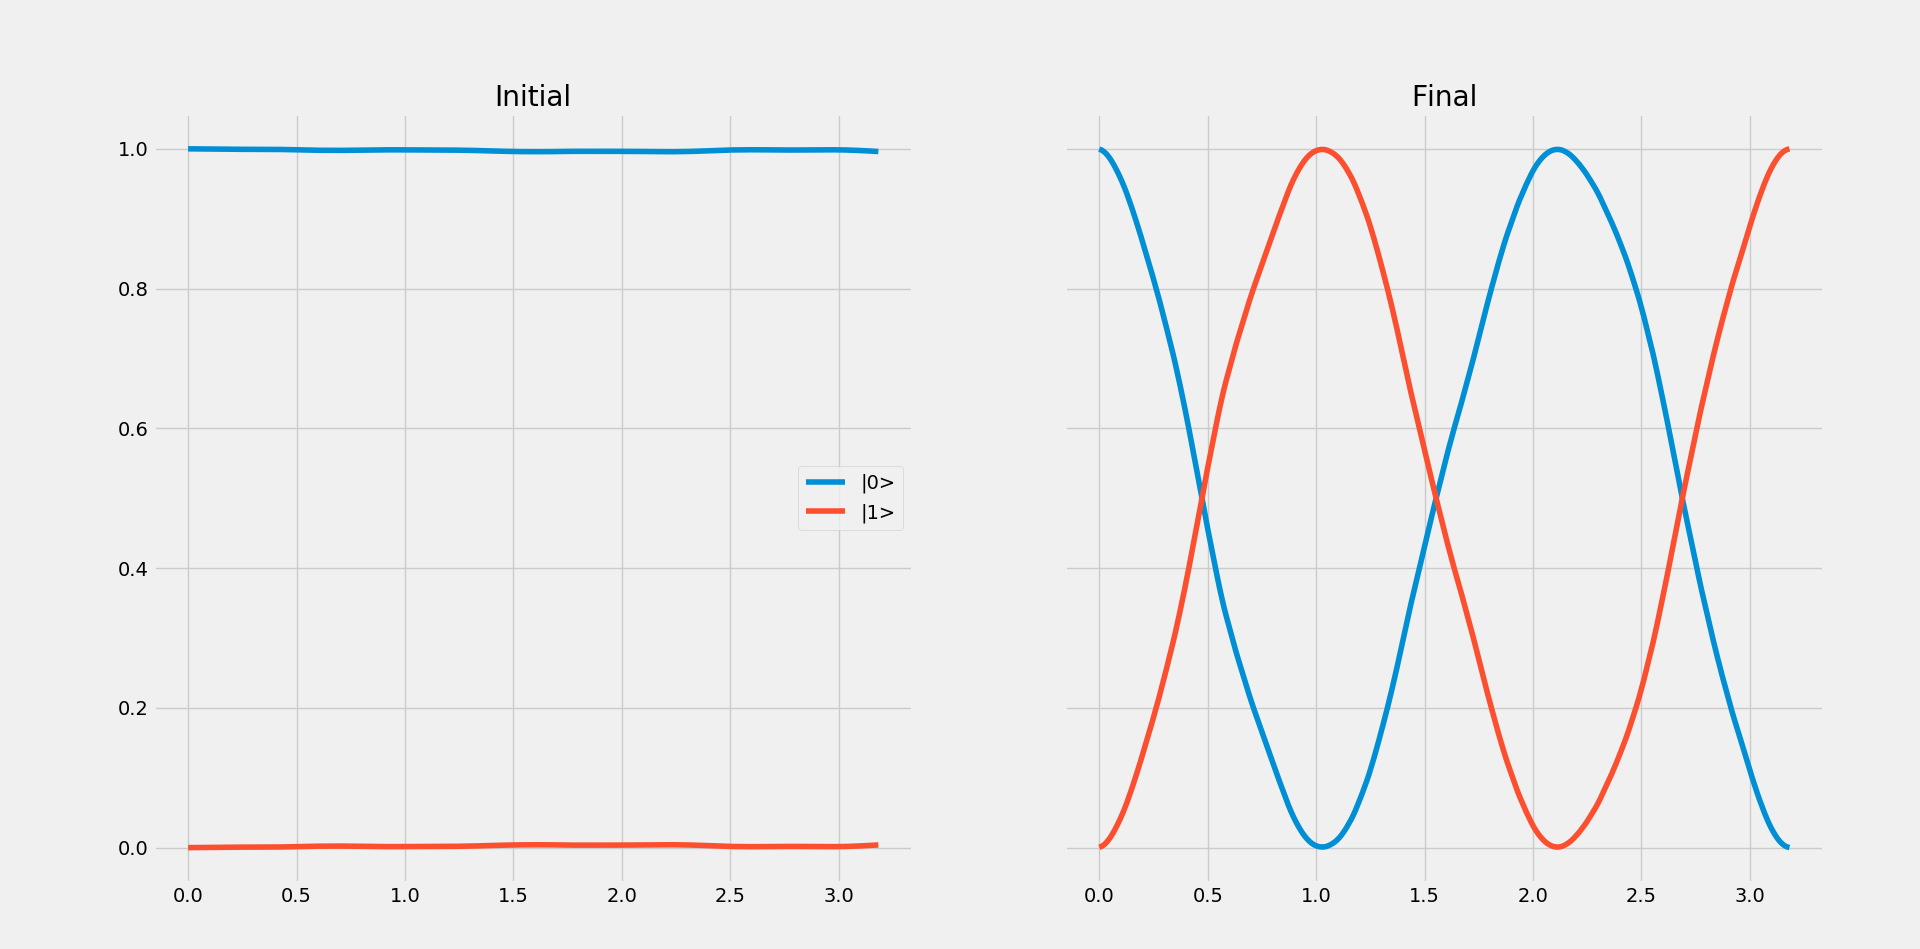
\includegraphics[width=0.9\columnwidth]{Results/No-Constraints-single-qubit/level-population-pretty2.png}
%     \end{center}
%     \caption{Population of qubit levels over pulse duration. Before the optimization, the state of the qubit (population of ground and excited states) almost did not change at all. After the optimization, the qubit goes from state $\ket{0}$ to $\ket{1}$ to $\ket{0}$ to $\ket{1}$, doing some unnecessary back and forth between the states}
%     \label{fig:GRAPE-first-example-level-population}
% \end{figure}
\begin{figure}[H]
    \begin{center}
        %% Creator: Matplotlib, PGF backend
%%
%% To include the figure in your LaTeX document, write
%%   \input{<filename>.pgf}
%%
%% Make sure the required packages are loaded in your preamble
%%   \usepackage{pgf}
%%
%% and, on pdftex
%%   \usepackage[utf8]{inputenc}\DeclareUnicodeCharacter{2212}{-}
%%
%% or, on luatex and xetex
%%   \usepackage{unicode-math}
%%
%% Figures using additional raster images can only be included by \input if
%% they are in the same directory as the main LaTeX file. For loading figures
%% from other directories you can use the `import` package
%%   \usepackage{import}
%%
%% and then include the figures with
%%   \import{<path to file>}{<filename>.pgf}
%%
%% Matplotlib used the following preamble
%%
\begingroup%
\makeatletter%
\begin{pgfpicture}%
\pgfpathrectangle{\pgfpointorigin}{\pgfqpoint{4.650000in}{2.300000in}}%
\pgfusepath{use as bounding box, clip}%
\begin{pgfscope}%
\pgfsetbuttcap%
\pgfsetmiterjoin%
\definecolor{currentfill}{rgb}{1.000000,1.000000,1.000000}%
\pgfsetfillcolor{currentfill}%
\pgfsetlinewidth{0.000000pt}%
\definecolor{currentstroke}{rgb}{1.000000,1.000000,1.000000}%
\pgfsetstrokecolor{currentstroke}%
\pgfsetdash{}{0pt}%
\pgfpathmoveto{\pgfqpoint{0.000000in}{0.000000in}}%
\pgfpathlineto{\pgfqpoint{4.650000in}{0.000000in}}%
\pgfpathlineto{\pgfqpoint{4.650000in}{2.300000in}}%
\pgfpathlineto{\pgfqpoint{0.000000in}{2.300000in}}%
\pgfpathclose%
\pgfusepath{fill}%
\end{pgfscope}%
\begin{pgfscope}%
\pgfsetbuttcap%
\pgfsetmiterjoin%
\definecolor{currentfill}{rgb}{1.000000,1.000000,1.000000}%
\pgfsetfillcolor{currentfill}%
\pgfsetlinewidth{0.000000pt}%
\definecolor{currentstroke}{rgb}{0.000000,0.000000,0.000000}%
\pgfsetstrokecolor{currentstroke}%
\pgfsetstrokeopacity{0.000000}%
\pgfsetdash{}{0pt}%
\pgfpathmoveto{\pgfqpoint{0.646914in}{0.370679in}}%
\pgfpathlineto{\pgfqpoint{2.474152in}{0.370679in}}%
\pgfpathlineto{\pgfqpoint{2.474152in}{1.927778in}}%
\pgfpathlineto{\pgfqpoint{0.646914in}{1.927778in}}%
\pgfpathclose%
\pgfusepath{fill}%
\end{pgfscope}%
\begin{pgfscope}%
\pgfpathrectangle{\pgfqpoint{0.646914in}{0.370679in}}{\pgfqpoint{1.827237in}{1.557099in}}%
\pgfusepath{clip}%
\pgfsetrectcap%
\pgfsetroundjoin%
\pgfsetlinewidth{0.803000pt}%
\definecolor{currentstroke}{rgb}{0.501961,0.501961,0.501961}%
\pgfsetstrokecolor{currentstroke}%
\pgfsetstrokeopacity{0.200000}%
\pgfsetdash{}{0pt}%
\pgfpathmoveto{\pgfqpoint{0.729970in}{0.370679in}}%
\pgfpathlineto{\pgfqpoint{0.729970in}{1.927778in}}%
\pgfusepath{stroke}%
\end{pgfscope}%
\begin{pgfscope}%
\pgfsetbuttcap%
\pgfsetroundjoin%
\definecolor{currentfill}{rgb}{0.333333,0.333333,0.333333}%
\pgfsetfillcolor{currentfill}%
\pgfsetlinewidth{0.803000pt}%
\definecolor{currentstroke}{rgb}{0.333333,0.333333,0.333333}%
\pgfsetstrokecolor{currentstroke}%
\pgfsetdash{}{0pt}%
\pgfsys@defobject{currentmarker}{\pgfqpoint{0.000000in}{-0.048611in}}{\pgfqpoint{0.000000in}{0.000000in}}{%
\pgfpathmoveto{\pgfqpoint{0.000000in}{0.000000in}}%
\pgfpathlineto{\pgfqpoint{0.000000in}{-0.048611in}}%
\pgfusepath{stroke,fill}%
}%
\begin{pgfscope}%
\pgfsys@transformshift{0.729970in}{0.370679in}%
\pgfsys@useobject{currentmarker}{}%
\end{pgfscope}%
\end{pgfscope}%
\begin{pgfscope}%
\definecolor{textcolor}{rgb}{0.333333,0.333333,0.333333}%
\pgfsetstrokecolor{textcolor}%
\pgfsetfillcolor{textcolor}%
\pgftext[x=0.729970in,y=0.273457in,,top]{\color{textcolor}\rmfamily\fontsize{10.000000}{12.000000}\selectfont \(\displaystyle {0}\)}%
\end{pgfscope}%
\begin{pgfscope}%
\pgfpathrectangle{\pgfqpoint{0.646914in}{0.370679in}}{\pgfqpoint{1.827237in}{1.557099in}}%
\pgfusepath{clip}%
\pgfsetrectcap%
\pgfsetroundjoin%
\pgfsetlinewidth{0.803000pt}%
\definecolor{currentstroke}{rgb}{0.501961,0.501961,0.501961}%
\pgfsetstrokecolor{currentstroke}%
\pgfsetstrokeopacity{0.200000}%
\pgfsetdash{}{0pt}%
\pgfpathmoveto{\pgfqpoint{1.394420in}{0.370679in}}%
\pgfpathlineto{\pgfqpoint{1.394420in}{1.927778in}}%
\pgfusepath{stroke}%
\end{pgfscope}%
\begin{pgfscope}%
\pgfsetbuttcap%
\pgfsetroundjoin%
\definecolor{currentfill}{rgb}{0.333333,0.333333,0.333333}%
\pgfsetfillcolor{currentfill}%
\pgfsetlinewidth{0.803000pt}%
\definecolor{currentstroke}{rgb}{0.333333,0.333333,0.333333}%
\pgfsetstrokecolor{currentstroke}%
\pgfsetdash{}{0pt}%
\pgfsys@defobject{currentmarker}{\pgfqpoint{0.000000in}{-0.048611in}}{\pgfqpoint{0.000000in}{0.000000in}}{%
\pgfpathmoveto{\pgfqpoint{0.000000in}{0.000000in}}%
\pgfpathlineto{\pgfqpoint{0.000000in}{-0.048611in}}%
\pgfusepath{stroke,fill}%
}%
\begin{pgfscope}%
\pgfsys@transformshift{1.394420in}{0.370679in}%
\pgfsys@useobject{currentmarker}{}%
\end{pgfscope}%
\end{pgfscope}%
\begin{pgfscope}%
\definecolor{textcolor}{rgb}{0.333333,0.333333,0.333333}%
\pgfsetstrokecolor{textcolor}%
\pgfsetfillcolor{textcolor}%
\pgftext[x=1.394420in,y=0.273457in,,top]{\color{textcolor}\rmfamily\fontsize{10.000000}{12.000000}\selectfont \(\displaystyle {10}\)}%
\end{pgfscope}%
\begin{pgfscope}%
\pgfpathrectangle{\pgfqpoint{0.646914in}{0.370679in}}{\pgfqpoint{1.827237in}{1.557099in}}%
\pgfusepath{clip}%
\pgfsetrectcap%
\pgfsetroundjoin%
\pgfsetlinewidth{0.803000pt}%
\definecolor{currentstroke}{rgb}{0.501961,0.501961,0.501961}%
\pgfsetstrokecolor{currentstroke}%
\pgfsetstrokeopacity{0.200000}%
\pgfsetdash{}{0pt}%
\pgfpathmoveto{\pgfqpoint{2.058870in}{0.370679in}}%
\pgfpathlineto{\pgfqpoint{2.058870in}{1.927778in}}%
\pgfusepath{stroke}%
\end{pgfscope}%
\begin{pgfscope}%
\pgfsetbuttcap%
\pgfsetroundjoin%
\definecolor{currentfill}{rgb}{0.333333,0.333333,0.333333}%
\pgfsetfillcolor{currentfill}%
\pgfsetlinewidth{0.803000pt}%
\definecolor{currentstroke}{rgb}{0.333333,0.333333,0.333333}%
\pgfsetstrokecolor{currentstroke}%
\pgfsetdash{}{0pt}%
\pgfsys@defobject{currentmarker}{\pgfqpoint{0.000000in}{-0.048611in}}{\pgfqpoint{0.000000in}{0.000000in}}{%
\pgfpathmoveto{\pgfqpoint{0.000000in}{0.000000in}}%
\pgfpathlineto{\pgfqpoint{0.000000in}{-0.048611in}}%
\pgfusepath{stroke,fill}%
}%
\begin{pgfscope}%
\pgfsys@transformshift{2.058870in}{0.370679in}%
\pgfsys@useobject{currentmarker}{}%
\end{pgfscope}%
\end{pgfscope}%
\begin{pgfscope}%
\definecolor{textcolor}{rgb}{0.333333,0.333333,0.333333}%
\pgfsetstrokecolor{textcolor}%
\pgfsetfillcolor{textcolor}%
\pgftext[x=2.058870in,y=0.273457in,,top]{\color{textcolor}\rmfamily\fontsize{10.000000}{12.000000}\selectfont \(\displaystyle {20}\)}%
\end{pgfscope}%
\begin{pgfscope}%
\pgfpathrectangle{\pgfqpoint{0.646914in}{0.370679in}}{\pgfqpoint{1.827237in}{1.557099in}}%
\pgfusepath{clip}%
\pgfsetrectcap%
\pgfsetroundjoin%
\pgfsetlinewidth{0.803000pt}%
\definecolor{currentstroke}{rgb}{0.501961,0.501961,0.501961}%
\pgfsetstrokecolor{currentstroke}%
\pgfsetstrokeopacity{0.200000}%
\pgfsetdash{}{0pt}%
\pgfpathmoveto{\pgfqpoint{0.646914in}{0.441456in}}%
\pgfpathlineto{\pgfqpoint{2.474152in}{0.441456in}}%
\pgfusepath{stroke}%
\end{pgfscope}%
\begin{pgfscope}%
\pgfsetbuttcap%
\pgfsetroundjoin%
\definecolor{currentfill}{rgb}{0.333333,0.333333,0.333333}%
\pgfsetfillcolor{currentfill}%
\pgfsetlinewidth{0.803000pt}%
\definecolor{currentstroke}{rgb}{0.333333,0.333333,0.333333}%
\pgfsetstrokecolor{currentstroke}%
\pgfsetdash{}{0pt}%
\pgfsys@defobject{currentmarker}{\pgfqpoint{-0.048611in}{0.000000in}}{\pgfqpoint{0.000000in}{0.000000in}}{%
\pgfpathmoveto{\pgfqpoint{0.000000in}{0.000000in}}%
\pgfpathlineto{\pgfqpoint{-0.048611in}{0.000000in}}%
\pgfusepath{stroke,fill}%
}%
\begin{pgfscope}%
\pgfsys@transformshift{0.646914in}{0.441456in}%
\pgfsys@useobject{currentmarker}{}%
\end{pgfscope}%
\end{pgfscope}%
\begin{pgfscope}%
\definecolor{textcolor}{rgb}{0.333333,0.333333,0.333333}%
\pgfsetstrokecolor{textcolor}%
\pgfsetfillcolor{textcolor}%
\pgftext[x=0.302778in, y=0.393231in, left, base]{\color{textcolor}\rmfamily\fontsize{10.000000}{12.000000}\selectfont \(\displaystyle {0.00}\)}%
\end{pgfscope}%
\begin{pgfscope}%
\pgfpathrectangle{\pgfqpoint{0.646914in}{0.370679in}}{\pgfqpoint{1.827237in}{1.557099in}}%
\pgfusepath{clip}%
\pgfsetrectcap%
\pgfsetroundjoin%
\pgfsetlinewidth{0.803000pt}%
\definecolor{currentstroke}{rgb}{0.501961,0.501961,0.501961}%
\pgfsetstrokecolor{currentstroke}%
\pgfsetstrokeopacity{0.200000}%
\pgfsetdash{}{0pt}%
\pgfpathmoveto{\pgfqpoint{0.646914in}{0.795342in}}%
\pgfpathlineto{\pgfqpoint{2.474152in}{0.795342in}}%
\pgfusepath{stroke}%
\end{pgfscope}%
\begin{pgfscope}%
\pgfsetbuttcap%
\pgfsetroundjoin%
\definecolor{currentfill}{rgb}{0.333333,0.333333,0.333333}%
\pgfsetfillcolor{currentfill}%
\pgfsetlinewidth{0.803000pt}%
\definecolor{currentstroke}{rgb}{0.333333,0.333333,0.333333}%
\pgfsetstrokecolor{currentstroke}%
\pgfsetdash{}{0pt}%
\pgfsys@defobject{currentmarker}{\pgfqpoint{-0.048611in}{0.000000in}}{\pgfqpoint{0.000000in}{0.000000in}}{%
\pgfpathmoveto{\pgfqpoint{0.000000in}{0.000000in}}%
\pgfpathlineto{\pgfqpoint{-0.048611in}{0.000000in}}%
\pgfusepath{stroke,fill}%
}%
\begin{pgfscope}%
\pgfsys@transformshift{0.646914in}{0.795342in}%
\pgfsys@useobject{currentmarker}{}%
\end{pgfscope}%
\end{pgfscope}%
\begin{pgfscope}%
\definecolor{textcolor}{rgb}{0.333333,0.333333,0.333333}%
\pgfsetstrokecolor{textcolor}%
\pgfsetfillcolor{textcolor}%
\pgftext[x=0.302778in, y=0.747117in, left, base]{\color{textcolor}\rmfamily\fontsize{10.000000}{12.000000}\selectfont \(\displaystyle {0.25}\)}%
\end{pgfscope}%
\begin{pgfscope}%
\pgfpathrectangle{\pgfqpoint{0.646914in}{0.370679in}}{\pgfqpoint{1.827237in}{1.557099in}}%
\pgfusepath{clip}%
\pgfsetrectcap%
\pgfsetroundjoin%
\pgfsetlinewidth{0.803000pt}%
\definecolor{currentstroke}{rgb}{0.501961,0.501961,0.501961}%
\pgfsetstrokecolor{currentstroke}%
\pgfsetstrokeopacity{0.200000}%
\pgfsetdash{}{0pt}%
\pgfpathmoveto{\pgfqpoint{0.646914in}{1.149228in}}%
\pgfpathlineto{\pgfqpoint{2.474152in}{1.149228in}}%
\pgfusepath{stroke}%
\end{pgfscope}%
\begin{pgfscope}%
\pgfsetbuttcap%
\pgfsetroundjoin%
\definecolor{currentfill}{rgb}{0.333333,0.333333,0.333333}%
\pgfsetfillcolor{currentfill}%
\pgfsetlinewidth{0.803000pt}%
\definecolor{currentstroke}{rgb}{0.333333,0.333333,0.333333}%
\pgfsetstrokecolor{currentstroke}%
\pgfsetdash{}{0pt}%
\pgfsys@defobject{currentmarker}{\pgfqpoint{-0.048611in}{0.000000in}}{\pgfqpoint{0.000000in}{0.000000in}}{%
\pgfpathmoveto{\pgfqpoint{0.000000in}{0.000000in}}%
\pgfpathlineto{\pgfqpoint{-0.048611in}{0.000000in}}%
\pgfusepath{stroke,fill}%
}%
\begin{pgfscope}%
\pgfsys@transformshift{0.646914in}{1.149228in}%
\pgfsys@useobject{currentmarker}{}%
\end{pgfscope}%
\end{pgfscope}%
\begin{pgfscope}%
\definecolor{textcolor}{rgb}{0.333333,0.333333,0.333333}%
\pgfsetstrokecolor{textcolor}%
\pgfsetfillcolor{textcolor}%
\pgftext[x=0.302778in, y=1.101003in, left, base]{\color{textcolor}\rmfamily\fontsize{10.000000}{12.000000}\selectfont \(\displaystyle {0.50}\)}%
\end{pgfscope}%
\begin{pgfscope}%
\pgfpathrectangle{\pgfqpoint{0.646914in}{0.370679in}}{\pgfqpoint{1.827237in}{1.557099in}}%
\pgfusepath{clip}%
\pgfsetrectcap%
\pgfsetroundjoin%
\pgfsetlinewidth{0.803000pt}%
\definecolor{currentstroke}{rgb}{0.501961,0.501961,0.501961}%
\pgfsetstrokecolor{currentstroke}%
\pgfsetstrokeopacity{0.200000}%
\pgfsetdash{}{0pt}%
\pgfpathmoveto{\pgfqpoint{0.646914in}{1.503115in}}%
\pgfpathlineto{\pgfqpoint{2.474152in}{1.503115in}}%
\pgfusepath{stroke}%
\end{pgfscope}%
\begin{pgfscope}%
\pgfsetbuttcap%
\pgfsetroundjoin%
\definecolor{currentfill}{rgb}{0.333333,0.333333,0.333333}%
\pgfsetfillcolor{currentfill}%
\pgfsetlinewidth{0.803000pt}%
\definecolor{currentstroke}{rgb}{0.333333,0.333333,0.333333}%
\pgfsetstrokecolor{currentstroke}%
\pgfsetdash{}{0pt}%
\pgfsys@defobject{currentmarker}{\pgfqpoint{-0.048611in}{0.000000in}}{\pgfqpoint{0.000000in}{0.000000in}}{%
\pgfpathmoveto{\pgfqpoint{0.000000in}{0.000000in}}%
\pgfpathlineto{\pgfqpoint{-0.048611in}{0.000000in}}%
\pgfusepath{stroke,fill}%
}%
\begin{pgfscope}%
\pgfsys@transformshift{0.646914in}{1.503115in}%
\pgfsys@useobject{currentmarker}{}%
\end{pgfscope}%
\end{pgfscope}%
\begin{pgfscope}%
\definecolor{textcolor}{rgb}{0.333333,0.333333,0.333333}%
\pgfsetstrokecolor{textcolor}%
\pgfsetfillcolor{textcolor}%
\pgftext[x=0.302778in, y=1.454889in, left, base]{\color{textcolor}\rmfamily\fontsize{10.000000}{12.000000}\selectfont \(\displaystyle {0.75}\)}%
\end{pgfscope}%
\begin{pgfscope}%
\pgfpathrectangle{\pgfqpoint{0.646914in}{0.370679in}}{\pgfqpoint{1.827237in}{1.557099in}}%
\pgfusepath{clip}%
\pgfsetrectcap%
\pgfsetroundjoin%
\pgfsetlinewidth{0.803000pt}%
\definecolor{currentstroke}{rgb}{0.501961,0.501961,0.501961}%
\pgfsetstrokecolor{currentstroke}%
\pgfsetstrokeopacity{0.200000}%
\pgfsetdash{}{0pt}%
\pgfpathmoveto{\pgfqpoint{0.646914in}{1.857001in}}%
\pgfpathlineto{\pgfqpoint{2.474152in}{1.857001in}}%
\pgfusepath{stroke}%
\end{pgfscope}%
\begin{pgfscope}%
\pgfsetbuttcap%
\pgfsetroundjoin%
\definecolor{currentfill}{rgb}{0.333333,0.333333,0.333333}%
\pgfsetfillcolor{currentfill}%
\pgfsetlinewidth{0.803000pt}%
\definecolor{currentstroke}{rgb}{0.333333,0.333333,0.333333}%
\pgfsetstrokecolor{currentstroke}%
\pgfsetdash{}{0pt}%
\pgfsys@defobject{currentmarker}{\pgfqpoint{-0.048611in}{0.000000in}}{\pgfqpoint{0.000000in}{0.000000in}}{%
\pgfpathmoveto{\pgfqpoint{0.000000in}{0.000000in}}%
\pgfpathlineto{\pgfqpoint{-0.048611in}{0.000000in}}%
\pgfusepath{stroke,fill}%
}%
\begin{pgfscope}%
\pgfsys@transformshift{0.646914in}{1.857001in}%
\pgfsys@useobject{currentmarker}{}%
\end{pgfscope}%
\end{pgfscope}%
\begin{pgfscope}%
\definecolor{textcolor}{rgb}{0.333333,0.333333,0.333333}%
\pgfsetstrokecolor{textcolor}%
\pgfsetfillcolor{textcolor}%
\pgftext[x=0.302778in, y=1.808776in, left, base]{\color{textcolor}\rmfamily\fontsize{10.000000}{12.000000}\selectfont \(\displaystyle {1.00}\)}%
\end{pgfscope}%
\begin{pgfscope}%
\definecolor{textcolor}{rgb}{0.333333,0.333333,0.333333}%
\pgfsetstrokecolor{textcolor}%
\pgfsetfillcolor{textcolor}%
\pgftext[x=0.247222in,y=1.149228in,,bottom,rotate=90.000000]{\color{textcolor}\rmfamily\fontsize{12.000000}{14.400000}\selectfont Amplitude (MHz)}%
\end{pgfscope}%
\begin{pgfscope}%
\pgfpathrectangle{\pgfqpoint{0.646914in}{0.370679in}}{\pgfqpoint{1.827237in}{1.557099in}}%
\pgfusepath{clip}%
\pgfsetrectcap%
\pgfsetroundjoin%
\pgfsetlinewidth{1.505625pt}%
\definecolor{currentstroke}{rgb}{0.886275,0.290196,0.200000}%
\pgfsetstrokecolor{currentstroke}%
\pgfsetdash{}{0pt}%
\pgfpathmoveto{\pgfqpoint{0.729970in}{1.857001in}}%
\pgfpathlineto{\pgfqpoint{2.391095in}{1.856987in}}%
\pgfpathlineto{\pgfqpoint{2.391095in}{1.856987in}}%
\pgfusepath{stroke}%
\end{pgfscope}%
\begin{pgfscope}%
\pgfpathrectangle{\pgfqpoint{0.646914in}{0.370679in}}{\pgfqpoint{1.827237in}{1.557099in}}%
\pgfusepath{clip}%
\pgfsetrectcap%
\pgfsetroundjoin%
\pgfsetlinewidth{1.505625pt}%
\definecolor{currentstroke}{rgb}{0.203922,0.541176,0.741176}%
\pgfsetstrokecolor{currentstroke}%
\pgfsetdash{}{0pt}%
\pgfpathmoveto{\pgfqpoint{0.729970in}{0.441456in}}%
\pgfpathlineto{\pgfqpoint{2.391095in}{0.441469in}}%
\pgfpathlineto{\pgfqpoint{2.391095in}{0.441469in}}%
\pgfusepath{stroke}%
\end{pgfscope}%
\begin{pgfscope}%
\pgfsetrectcap%
\pgfsetmiterjoin%
\pgfsetlinewidth{1.003750pt}%
\definecolor{currentstroke}{rgb}{1.000000,1.000000,1.000000}%
\pgfsetstrokecolor{currentstroke}%
\pgfsetdash{}{0pt}%
\pgfpathmoveto{\pgfqpoint{0.646914in}{0.370679in}}%
\pgfpathlineto{\pgfqpoint{0.646914in}{1.927778in}}%
\pgfusepath{stroke}%
\end{pgfscope}%
\begin{pgfscope}%
\pgfsetrectcap%
\pgfsetmiterjoin%
\pgfsetlinewidth{1.003750pt}%
\definecolor{currentstroke}{rgb}{1.000000,1.000000,1.000000}%
\pgfsetstrokecolor{currentstroke}%
\pgfsetdash{}{0pt}%
\pgfpathmoveto{\pgfqpoint{2.474152in}{0.370679in}}%
\pgfpathlineto{\pgfqpoint{2.474152in}{1.927778in}}%
\pgfusepath{stroke}%
\end{pgfscope}%
\begin{pgfscope}%
\pgfsetrectcap%
\pgfsetmiterjoin%
\pgfsetlinewidth{1.003750pt}%
\definecolor{currentstroke}{rgb}{1.000000,1.000000,1.000000}%
\pgfsetstrokecolor{currentstroke}%
\pgfsetdash{}{0pt}%
\pgfpathmoveto{\pgfqpoint{0.646914in}{0.370679in}}%
\pgfpathlineto{\pgfqpoint{2.474152in}{0.370679in}}%
\pgfusepath{stroke}%
\end{pgfscope}%
\begin{pgfscope}%
\pgfsetrectcap%
\pgfsetmiterjoin%
\pgfsetlinewidth{1.003750pt}%
\definecolor{currentstroke}{rgb}{1.000000,1.000000,1.000000}%
\pgfsetstrokecolor{currentstroke}%
\pgfsetdash{}{0pt}%
\pgfpathmoveto{\pgfqpoint{0.646914in}{1.927778in}}%
\pgfpathlineto{\pgfqpoint{2.474152in}{1.927778in}}%
\pgfusepath{stroke}%
\end{pgfscope}%
\begin{pgfscope}%
\definecolor{textcolor}{rgb}{0.000000,0.000000,0.000000}%
\pgfsetstrokecolor{textcolor}%
\pgfsetfillcolor{textcolor}%
\pgftext[x=1.560533in,y=2.011111in,,base]{\color{textcolor}\rmfamily\fontsize{14.400000}{17.280000}\selectfont Initial pulse}%
\end{pgfscope}%
\begin{pgfscope}%
\pgfsetbuttcap%
\pgfsetmiterjoin%
\definecolor{currentfill}{rgb}{1.000000,1.000000,1.000000}%
\pgfsetfillcolor{currentfill}%
\pgfsetfillopacity{0.800000}%
\pgfsetlinewidth{0.501875pt}%
\definecolor{currentstroke}{rgb}{0.800000,0.800000,0.800000}%
\pgfsetstrokecolor{currentstroke}%
\pgfsetstrokeopacity{0.800000}%
\pgfsetdash{}{0pt}%
\pgfpathmoveto{\pgfqpoint{1.552179in}{0.920062in}}%
\pgfpathlineto{\pgfqpoint{2.376929in}{0.920062in}}%
\pgfpathquadraticcurveto{\pgfqpoint{2.404707in}{0.920062in}}{\pgfqpoint{2.404707in}{0.947840in}}%
\pgfpathlineto{\pgfqpoint{2.404707in}{1.350617in}}%
\pgfpathquadraticcurveto{\pgfqpoint{2.404707in}{1.378395in}}{\pgfqpoint{2.376929in}{1.378395in}}%
\pgfpathlineto{\pgfqpoint{1.552179in}{1.378395in}}%
\pgfpathquadraticcurveto{\pgfqpoint{1.524402in}{1.378395in}}{\pgfqpoint{1.524402in}{1.350617in}}%
\pgfpathlineto{\pgfqpoint{1.524402in}{0.947840in}}%
\pgfpathquadraticcurveto{\pgfqpoint{1.524402in}{0.920062in}}{\pgfqpoint{1.552179in}{0.920062in}}%
\pgfpathclose%
\pgfusepath{stroke,fill}%
\end{pgfscope}%
\begin{pgfscope}%
\pgfsetrectcap%
\pgfsetroundjoin%
\pgfsetlinewidth{1.505625pt}%
\definecolor{currentstroke}{rgb}{0.886275,0.290196,0.200000}%
\pgfsetstrokecolor{currentstroke}%
\pgfsetdash{}{0pt}%
\pgfpathmoveto{\pgfqpoint{1.579957in}{1.267284in}}%
\pgfpathlineto{\pgfqpoint{1.857735in}{1.267284in}}%
\pgfusepath{stroke}%
\end{pgfscope}%
\begin{pgfscope}%
\definecolor{textcolor}{rgb}{0.000000,0.000000,0.000000}%
\pgfsetstrokecolor{textcolor}%
\pgfsetfillcolor{textcolor}%
\pgftext[x=1.968846in,y=1.218673in,left,base]{\color{textcolor}\rmfamily\fontsize{10.000000}{12.000000}\selectfont \(\displaystyle P(|g\rangle)\)}%
\end{pgfscope}%
\begin{pgfscope}%
\pgfsetrectcap%
\pgfsetroundjoin%
\pgfsetlinewidth{1.505625pt}%
\definecolor{currentstroke}{rgb}{0.203922,0.541176,0.741176}%
\pgfsetstrokecolor{currentstroke}%
\pgfsetdash{}{0pt}%
\pgfpathmoveto{\pgfqpoint{1.579957in}{1.058951in}}%
\pgfpathlineto{\pgfqpoint{1.857735in}{1.058951in}}%
\pgfusepath{stroke}%
\end{pgfscope}%
\begin{pgfscope}%
\definecolor{textcolor}{rgb}{0.000000,0.000000,0.000000}%
\pgfsetstrokecolor{textcolor}%
\pgfsetfillcolor{textcolor}%
\pgftext[x=1.968846in,y=1.010340in,left,base]{\color{textcolor}\rmfamily\fontsize{10.000000}{12.000000}\selectfont \(\displaystyle P(|e\rangle)\)}%
\end{pgfscope}%
\begin{pgfscope}%
\pgfsetbuttcap%
\pgfsetmiterjoin%
\definecolor{currentfill}{rgb}{1.000000,1.000000,1.000000}%
\pgfsetfillcolor{currentfill}%
\pgfsetlinewidth{0.000000pt}%
\definecolor{currentstroke}{rgb}{0.000000,0.000000,0.000000}%
\pgfsetstrokecolor{currentstroke}%
\pgfsetstrokeopacity{0.000000}%
\pgfsetdash{}{0pt}%
\pgfpathmoveto{\pgfqpoint{2.672763in}{0.370679in}}%
\pgfpathlineto{\pgfqpoint{4.500000in}{0.370679in}}%
\pgfpathlineto{\pgfqpoint{4.500000in}{1.927778in}}%
\pgfpathlineto{\pgfqpoint{2.672763in}{1.927778in}}%
\pgfpathclose%
\pgfusepath{fill}%
\end{pgfscope}%
\begin{pgfscope}%
\pgfpathrectangle{\pgfqpoint{2.672763in}{0.370679in}}{\pgfqpoint{1.827237in}{1.557099in}}%
\pgfusepath{clip}%
\pgfsetrectcap%
\pgfsetroundjoin%
\pgfsetlinewidth{0.803000pt}%
\definecolor{currentstroke}{rgb}{0.501961,0.501961,0.501961}%
\pgfsetstrokecolor{currentstroke}%
\pgfsetstrokeopacity{0.200000}%
\pgfsetdash{}{0pt}%
\pgfpathmoveto{\pgfqpoint{2.755819in}{0.370679in}}%
\pgfpathlineto{\pgfqpoint{2.755819in}{1.927778in}}%
\pgfusepath{stroke}%
\end{pgfscope}%
\begin{pgfscope}%
\pgfsetbuttcap%
\pgfsetroundjoin%
\definecolor{currentfill}{rgb}{0.333333,0.333333,0.333333}%
\pgfsetfillcolor{currentfill}%
\pgfsetlinewidth{0.803000pt}%
\definecolor{currentstroke}{rgb}{0.333333,0.333333,0.333333}%
\pgfsetstrokecolor{currentstroke}%
\pgfsetdash{}{0pt}%
\pgfsys@defobject{currentmarker}{\pgfqpoint{0.000000in}{-0.048611in}}{\pgfqpoint{0.000000in}{0.000000in}}{%
\pgfpathmoveto{\pgfqpoint{0.000000in}{0.000000in}}%
\pgfpathlineto{\pgfqpoint{0.000000in}{-0.048611in}}%
\pgfusepath{stroke,fill}%
}%
\begin{pgfscope}%
\pgfsys@transformshift{2.755819in}{0.370679in}%
\pgfsys@useobject{currentmarker}{}%
\end{pgfscope}%
\end{pgfscope}%
\begin{pgfscope}%
\definecolor{textcolor}{rgb}{0.333333,0.333333,0.333333}%
\pgfsetstrokecolor{textcolor}%
\pgfsetfillcolor{textcolor}%
\pgftext[x=2.755819in,y=0.273457in,,top]{\color{textcolor}\rmfamily\fontsize{10.000000}{12.000000}\selectfont \(\displaystyle {0}\)}%
\end{pgfscope}%
\begin{pgfscope}%
\pgfpathrectangle{\pgfqpoint{2.672763in}{0.370679in}}{\pgfqpoint{1.827237in}{1.557099in}}%
\pgfusepath{clip}%
\pgfsetrectcap%
\pgfsetroundjoin%
\pgfsetlinewidth{0.803000pt}%
\definecolor{currentstroke}{rgb}{0.501961,0.501961,0.501961}%
\pgfsetstrokecolor{currentstroke}%
\pgfsetstrokeopacity{0.200000}%
\pgfsetdash{}{0pt}%
\pgfpathmoveto{\pgfqpoint{3.420269in}{0.370679in}}%
\pgfpathlineto{\pgfqpoint{3.420269in}{1.927778in}}%
\pgfusepath{stroke}%
\end{pgfscope}%
\begin{pgfscope}%
\pgfsetbuttcap%
\pgfsetroundjoin%
\definecolor{currentfill}{rgb}{0.333333,0.333333,0.333333}%
\pgfsetfillcolor{currentfill}%
\pgfsetlinewidth{0.803000pt}%
\definecolor{currentstroke}{rgb}{0.333333,0.333333,0.333333}%
\pgfsetstrokecolor{currentstroke}%
\pgfsetdash{}{0pt}%
\pgfsys@defobject{currentmarker}{\pgfqpoint{0.000000in}{-0.048611in}}{\pgfqpoint{0.000000in}{0.000000in}}{%
\pgfpathmoveto{\pgfqpoint{0.000000in}{0.000000in}}%
\pgfpathlineto{\pgfqpoint{0.000000in}{-0.048611in}}%
\pgfusepath{stroke,fill}%
}%
\begin{pgfscope}%
\pgfsys@transformshift{3.420269in}{0.370679in}%
\pgfsys@useobject{currentmarker}{}%
\end{pgfscope}%
\end{pgfscope}%
\begin{pgfscope}%
\definecolor{textcolor}{rgb}{0.333333,0.333333,0.333333}%
\pgfsetstrokecolor{textcolor}%
\pgfsetfillcolor{textcolor}%
\pgftext[x=3.420269in,y=0.273457in,,top]{\color{textcolor}\rmfamily\fontsize{10.000000}{12.000000}\selectfont \(\displaystyle {10}\)}%
\end{pgfscope}%
\begin{pgfscope}%
\pgfpathrectangle{\pgfqpoint{2.672763in}{0.370679in}}{\pgfqpoint{1.827237in}{1.557099in}}%
\pgfusepath{clip}%
\pgfsetrectcap%
\pgfsetroundjoin%
\pgfsetlinewidth{0.803000pt}%
\definecolor{currentstroke}{rgb}{0.501961,0.501961,0.501961}%
\pgfsetstrokecolor{currentstroke}%
\pgfsetstrokeopacity{0.200000}%
\pgfsetdash{}{0pt}%
\pgfpathmoveto{\pgfqpoint{4.084719in}{0.370679in}}%
\pgfpathlineto{\pgfqpoint{4.084719in}{1.927778in}}%
\pgfusepath{stroke}%
\end{pgfscope}%
\begin{pgfscope}%
\pgfsetbuttcap%
\pgfsetroundjoin%
\definecolor{currentfill}{rgb}{0.333333,0.333333,0.333333}%
\pgfsetfillcolor{currentfill}%
\pgfsetlinewidth{0.803000pt}%
\definecolor{currentstroke}{rgb}{0.333333,0.333333,0.333333}%
\pgfsetstrokecolor{currentstroke}%
\pgfsetdash{}{0pt}%
\pgfsys@defobject{currentmarker}{\pgfqpoint{0.000000in}{-0.048611in}}{\pgfqpoint{0.000000in}{0.000000in}}{%
\pgfpathmoveto{\pgfqpoint{0.000000in}{0.000000in}}%
\pgfpathlineto{\pgfqpoint{0.000000in}{-0.048611in}}%
\pgfusepath{stroke,fill}%
}%
\begin{pgfscope}%
\pgfsys@transformshift{4.084719in}{0.370679in}%
\pgfsys@useobject{currentmarker}{}%
\end{pgfscope}%
\end{pgfscope}%
\begin{pgfscope}%
\definecolor{textcolor}{rgb}{0.333333,0.333333,0.333333}%
\pgfsetstrokecolor{textcolor}%
\pgfsetfillcolor{textcolor}%
\pgftext[x=4.084719in,y=0.273457in,,top]{\color{textcolor}\rmfamily\fontsize{10.000000}{12.000000}\selectfont \(\displaystyle {20}\)}%
\end{pgfscope}%
\begin{pgfscope}%
\pgfpathrectangle{\pgfqpoint{2.672763in}{0.370679in}}{\pgfqpoint{1.827237in}{1.557099in}}%
\pgfusepath{clip}%
\pgfsetrectcap%
\pgfsetroundjoin%
\pgfsetlinewidth{0.803000pt}%
\definecolor{currentstroke}{rgb}{0.501961,0.501961,0.501961}%
\pgfsetstrokecolor{currentstroke}%
\pgfsetstrokeopacity{0.200000}%
\pgfsetdash{}{0pt}%
\pgfpathmoveto{\pgfqpoint{2.672763in}{0.441456in}}%
\pgfpathlineto{\pgfqpoint{4.500000in}{0.441456in}}%
\pgfusepath{stroke}%
\end{pgfscope}%
\begin{pgfscope}%
\pgfsetbuttcap%
\pgfsetroundjoin%
\definecolor{currentfill}{rgb}{0.333333,0.333333,0.333333}%
\pgfsetfillcolor{currentfill}%
\pgfsetlinewidth{0.803000pt}%
\definecolor{currentstroke}{rgb}{0.333333,0.333333,0.333333}%
\pgfsetstrokecolor{currentstroke}%
\pgfsetdash{}{0pt}%
\pgfsys@defobject{currentmarker}{\pgfqpoint{-0.048611in}{0.000000in}}{\pgfqpoint{0.000000in}{0.000000in}}{%
\pgfpathmoveto{\pgfqpoint{0.000000in}{0.000000in}}%
\pgfpathlineto{\pgfqpoint{-0.048611in}{0.000000in}}%
\pgfusepath{stroke,fill}%
}%
\begin{pgfscope}%
\pgfsys@transformshift{2.672763in}{0.441456in}%
\pgfsys@useobject{currentmarker}{}%
\end{pgfscope}%
\end{pgfscope}%
\begin{pgfscope}%
\pgfpathrectangle{\pgfqpoint{2.672763in}{0.370679in}}{\pgfqpoint{1.827237in}{1.557099in}}%
\pgfusepath{clip}%
\pgfsetrectcap%
\pgfsetroundjoin%
\pgfsetlinewidth{0.803000pt}%
\definecolor{currentstroke}{rgb}{0.501961,0.501961,0.501961}%
\pgfsetstrokecolor{currentstroke}%
\pgfsetstrokeopacity{0.200000}%
\pgfsetdash{}{0pt}%
\pgfpathmoveto{\pgfqpoint{2.672763in}{0.795342in}}%
\pgfpathlineto{\pgfqpoint{4.500000in}{0.795342in}}%
\pgfusepath{stroke}%
\end{pgfscope}%
\begin{pgfscope}%
\pgfsetbuttcap%
\pgfsetroundjoin%
\definecolor{currentfill}{rgb}{0.333333,0.333333,0.333333}%
\pgfsetfillcolor{currentfill}%
\pgfsetlinewidth{0.803000pt}%
\definecolor{currentstroke}{rgb}{0.333333,0.333333,0.333333}%
\pgfsetstrokecolor{currentstroke}%
\pgfsetdash{}{0pt}%
\pgfsys@defobject{currentmarker}{\pgfqpoint{-0.048611in}{0.000000in}}{\pgfqpoint{0.000000in}{0.000000in}}{%
\pgfpathmoveto{\pgfqpoint{0.000000in}{0.000000in}}%
\pgfpathlineto{\pgfqpoint{-0.048611in}{0.000000in}}%
\pgfusepath{stroke,fill}%
}%
\begin{pgfscope}%
\pgfsys@transformshift{2.672763in}{0.795342in}%
\pgfsys@useobject{currentmarker}{}%
\end{pgfscope}%
\end{pgfscope}%
\begin{pgfscope}%
\pgfpathrectangle{\pgfqpoint{2.672763in}{0.370679in}}{\pgfqpoint{1.827237in}{1.557099in}}%
\pgfusepath{clip}%
\pgfsetrectcap%
\pgfsetroundjoin%
\pgfsetlinewidth{0.803000pt}%
\definecolor{currentstroke}{rgb}{0.501961,0.501961,0.501961}%
\pgfsetstrokecolor{currentstroke}%
\pgfsetstrokeopacity{0.200000}%
\pgfsetdash{}{0pt}%
\pgfpathmoveto{\pgfqpoint{2.672763in}{1.149228in}}%
\pgfpathlineto{\pgfqpoint{4.500000in}{1.149228in}}%
\pgfusepath{stroke}%
\end{pgfscope}%
\begin{pgfscope}%
\pgfsetbuttcap%
\pgfsetroundjoin%
\definecolor{currentfill}{rgb}{0.333333,0.333333,0.333333}%
\pgfsetfillcolor{currentfill}%
\pgfsetlinewidth{0.803000pt}%
\definecolor{currentstroke}{rgb}{0.333333,0.333333,0.333333}%
\pgfsetstrokecolor{currentstroke}%
\pgfsetdash{}{0pt}%
\pgfsys@defobject{currentmarker}{\pgfqpoint{-0.048611in}{0.000000in}}{\pgfqpoint{0.000000in}{0.000000in}}{%
\pgfpathmoveto{\pgfqpoint{0.000000in}{0.000000in}}%
\pgfpathlineto{\pgfqpoint{-0.048611in}{0.000000in}}%
\pgfusepath{stroke,fill}%
}%
\begin{pgfscope}%
\pgfsys@transformshift{2.672763in}{1.149228in}%
\pgfsys@useobject{currentmarker}{}%
\end{pgfscope}%
\end{pgfscope}%
\begin{pgfscope}%
\pgfpathrectangle{\pgfqpoint{2.672763in}{0.370679in}}{\pgfqpoint{1.827237in}{1.557099in}}%
\pgfusepath{clip}%
\pgfsetrectcap%
\pgfsetroundjoin%
\pgfsetlinewidth{0.803000pt}%
\definecolor{currentstroke}{rgb}{0.501961,0.501961,0.501961}%
\pgfsetstrokecolor{currentstroke}%
\pgfsetstrokeopacity{0.200000}%
\pgfsetdash{}{0pt}%
\pgfpathmoveto{\pgfqpoint{2.672763in}{1.503115in}}%
\pgfpathlineto{\pgfqpoint{4.500000in}{1.503115in}}%
\pgfusepath{stroke}%
\end{pgfscope}%
\begin{pgfscope}%
\pgfsetbuttcap%
\pgfsetroundjoin%
\definecolor{currentfill}{rgb}{0.333333,0.333333,0.333333}%
\pgfsetfillcolor{currentfill}%
\pgfsetlinewidth{0.803000pt}%
\definecolor{currentstroke}{rgb}{0.333333,0.333333,0.333333}%
\pgfsetstrokecolor{currentstroke}%
\pgfsetdash{}{0pt}%
\pgfsys@defobject{currentmarker}{\pgfqpoint{-0.048611in}{0.000000in}}{\pgfqpoint{0.000000in}{0.000000in}}{%
\pgfpathmoveto{\pgfqpoint{0.000000in}{0.000000in}}%
\pgfpathlineto{\pgfqpoint{-0.048611in}{0.000000in}}%
\pgfusepath{stroke,fill}%
}%
\begin{pgfscope}%
\pgfsys@transformshift{2.672763in}{1.503115in}%
\pgfsys@useobject{currentmarker}{}%
\end{pgfscope}%
\end{pgfscope}%
\begin{pgfscope}%
\pgfpathrectangle{\pgfqpoint{2.672763in}{0.370679in}}{\pgfqpoint{1.827237in}{1.557099in}}%
\pgfusepath{clip}%
\pgfsetrectcap%
\pgfsetroundjoin%
\pgfsetlinewidth{0.803000pt}%
\definecolor{currentstroke}{rgb}{0.501961,0.501961,0.501961}%
\pgfsetstrokecolor{currentstroke}%
\pgfsetstrokeopacity{0.200000}%
\pgfsetdash{}{0pt}%
\pgfpathmoveto{\pgfqpoint{2.672763in}{1.857001in}}%
\pgfpathlineto{\pgfqpoint{4.500000in}{1.857001in}}%
\pgfusepath{stroke}%
\end{pgfscope}%
\begin{pgfscope}%
\pgfsetbuttcap%
\pgfsetroundjoin%
\definecolor{currentfill}{rgb}{0.333333,0.333333,0.333333}%
\pgfsetfillcolor{currentfill}%
\pgfsetlinewidth{0.803000pt}%
\definecolor{currentstroke}{rgb}{0.333333,0.333333,0.333333}%
\pgfsetstrokecolor{currentstroke}%
\pgfsetdash{}{0pt}%
\pgfsys@defobject{currentmarker}{\pgfqpoint{-0.048611in}{0.000000in}}{\pgfqpoint{0.000000in}{0.000000in}}{%
\pgfpathmoveto{\pgfqpoint{0.000000in}{0.000000in}}%
\pgfpathlineto{\pgfqpoint{-0.048611in}{0.000000in}}%
\pgfusepath{stroke,fill}%
}%
\begin{pgfscope}%
\pgfsys@transformshift{2.672763in}{1.857001in}%
\pgfsys@useobject{currentmarker}{}%
\end{pgfscope}%
\end{pgfscope}%
\begin{pgfscope}%
\pgfpathrectangle{\pgfqpoint{2.672763in}{0.370679in}}{\pgfqpoint{1.827237in}{1.557099in}}%
\pgfusepath{clip}%
\pgfsetrectcap%
\pgfsetroundjoin%
\pgfsetlinewidth{1.505625pt}%
\definecolor{currentstroke}{rgb}{0.886275,0.290196,0.200000}%
\pgfsetstrokecolor{currentstroke}%
\pgfsetdash{}{0pt}%
\pgfpathmoveto{\pgfqpoint{2.755819in}{1.856915in}}%
\pgfpathlineto{\pgfqpoint{2.789208in}{1.854853in}}%
\pgfpathlineto{\pgfqpoint{2.822598in}{1.849998in}}%
\pgfpathlineto{\pgfqpoint{2.855987in}{1.842205in}}%
\pgfpathlineto{\pgfqpoint{2.889377in}{1.831577in}}%
\pgfpathlineto{\pgfqpoint{2.922766in}{1.818382in}}%
\pgfpathlineto{\pgfqpoint{2.964503in}{1.797995in}}%
\pgfpathlineto{\pgfqpoint{3.006240in}{1.773568in}}%
\pgfpathlineto{\pgfqpoint{3.047977in}{1.745323in}}%
\pgfpathlineto{\pgfqpoint{3.098061in}{1.707292in}}%
\pgfpathlineto{\pgfqpoint{3.148145in}{1.663981in}}%
\pgfpathlineto{\pgfqpoint{3.189882in}{1.624561in}}%
\pgfpathlineto{\pgfqpoint{3.239966in}{1.573058in}}%
\pgfpathlineto{\pgfqpoint{3.298397in}{1.508591in}}%
\pgfpathlineto{\pgfqpoint{3.348482in}{1.449914in}}%
\pgfpathlineto{\pgfqpoint{3.415260in}{1.365946in}}%
\pgfpathlineto{\pgfqpoint{3.565513in}{1.170061in}}%
\pgfpathlineto{\pgfqpoint{3.732460in}{0.950177in}}%
\pgfpathlineto{\pgfqpoint{3.815934in}{0.847804in}}%
\pgfpathlineto{\pgfqpoint{3.891060in}{0.761994in}}%
\pgfpathlineto{\pgfqpoint{3.949492in}{0.699613in}}%
\pgfpathlineto{\pgfqpoint{3.999576in}{0.649561in}}%
\pgfpathlineto{\pgfqpoint{4.049660in}{0.604309in}}%
\pgfpathlineto{\pgfqpoint{4.091397in}{0.570493in}}%
\pgfpathlineto{\pgfqpoint{4.141481in}{0.534391in}}%
\pgfpathlineto{\pgfqpoint{4.183218in}{0.508237in}}%
\pgfpathlineto{\pgfqpoint{4.224954in}{0.486459in}}%
\pgfpathlineto{\pgfqpoint{4.258344in}{0.472265in}}%
\pgfpathlineto{\pgfqpoint{4.300081in}{0.458408in}}%
\pgfpathlineto{\pgfqpoint{4.333470in}{0.450132in}}%
\pgfpathlineto{\pgfqpoint{4.366860in}{0.444555in}}%
\pgfpathlineto{\pgfqpoint{4.400249in}{0.441789in}}%
\pgfpathlineto{\pgfqpoint{4.416944in}{0.441456in}}%
\pgfpathlineto{\pgfqpoint{4.416944in}{0.441456in}}%
\pgfusepath{stroke}%
\end{pgfscope}%
\begin{pgfscope}%
\pgfpathrectangle{\pgfqpoint{2.672763in}{0.370679in}}{\pgfqpoint{1.827237in}{1.557099in}}%
\pgfusepath{clip}%
\pgfsetrectcap%
\pgfsetroundjoin%
\pgfsetlinewidth{1.505625pt}%
\definecolor{currentstroke}{rgb}{0.203922,0.541176,0.741176}%
\pgfsetstrokecolor{currentstroke}%
\pgfsetdash{}{0pt}%
\pgfpathmoveto{\pgfqpoint{2.755819in}{0.441542in}}%
\pgfpathlineto{\pgfqpoint{2.789208in}{0.443604in}}%
\pgfpathlineto{\pgfqpoint{2.822598in}{0.448458in}}%
\pgfpathlineto{\pgfqpoint{2.855987in}{0.456252in}}%
\pgfpathlineto{\pgfqpoint{2.889377in}{0.466880in}}%
\pgfpathlineto{\pgfqpoint{2.922766in}{0.480075in}}%
\pgfpathlineto{\pgfqpoint{2.964503in}{0.500462in}}%
\pgfpathlineto{\pgfqpoint{3.006240in}{0.524888in}}%
\pgfpathlineto{\pgfqpoint{3.047977in}{0.553134in}}%
\pgfpathlineto{\pgfqpoint{3.098061in}{0.591165in}}%
\pgfpathlineto{\pgfqpoint{3.148145in}{0.634476in}}%
\pgfpathlineto{\pgfqpoint{3.189882in}{0.673896in}}%
\pgfpathlineto{\pgfqpoint{3.239966in}{0.725399in}}%
\pgfpathlineto{\pgfqpoint{3.298397in}{0.789866in}}%
\pgfpathlineto{\pgfqpoint{3.348482in}{0.848543in}}%
\pgfpathlineto{\pgfqpoint{3.415260in}{0.932511in}}%
\pgfpathlineto{\pgfqpoint{3.565513in}{1.128396in}}%
\pgfpathlineto{\pgfqpoint{3.732460in}{1.348280in}}%
\pgfpathlineto{\pgfqpoint{3.815934in}{1.450653in}}%
\pgfpathlineto{\pgfqpoint{3.891060in}{1.536463in}}%
\pgfpathlineto{\pgfqpoint{3.949492in}{1.598844in}}%
\pgfpathlineto{\pgfqpoint{3.999576in}{1.648896in}}%
\pgfpathlineto{\pgfqpoint{4.049660in}{1.694148in}}%
\pgfpathlineto{\pgfqpoint{4.091397in}{1.727964in}}%
\pgfpathlineto{\pgfqpoint{4.141481in}{1.764065in}}%
\pgfpathlineto{\pgfqpoint{4.183218in}{1.790220in}}%
\pgfpathlineto{\pgfqpoint{4.224954in}{1.811998in}}%
\pgfpathlineto{\pgfqpoint{4.258344in}{1.826192in}}%
\pgfpathlineto{\pgfqpoint{4.300081in}{1.840049in}}%
\pgfpathlineto{\pgfqpoint{4.333470in}{1.848325in}}%
\pgfpathlineto{\pgfqpoint{4.366860in}{1.853902in}}%
\pgfpathlineto{\pgfqpoint{4.400249in}{1.856668in}}%
\pgfpathlineto{\pgfqpoint{4.416944in}{1.857001in}}%
\pgfpathlineto{\pgfqpoint{4.416944in}{1.857001in}}%
\pgfusepath{stroke}%
\end{pgfscope}%
\begin{pgfscope}%
\pgfsetrectcap%
\pgfsetmiterjoin%
\pgfsetlinewidth{1.003750pt}%
\definecolor{currentstroke}{rgb}{1.000000,1.000000,1.000000}%
\pgfsetstrokecolor{currentstroke}%
\pgfsetdash{}{0pt}%
\pgfpathmoveto{\pgfqpoint{2.672763in}{0.370679in}}%
\pgfpathlineto{\pgfqpoint{2.672763in}{1.927778in}}%
\pgfusepath{stroke}%
\end{pgfscope}%
\begin{pgfscope}%
\pgfsetrectcap%
\pgfsetmiterjoin%
\pgfsetlinewidth{1.003750pt}%
\definecolor{currentstroke}{rgb}{1.000000,1.000000,1.000000}%
\pgfsetstrokecolor{currentstroke}%
\pgfsetdash{}{0pt}%
\pgfpathmoveto{\pgfqpoint{4.500000in}{0.370679in}}%
\pgfpathlineto{\pgfqpoint{4.500000in}{1.927778in}}%
\pgfusepath{stroke}%
\end{pgfscope}%
\begin{pgfscope}%
\pgfsetrectcap%
\pgfsetmiterjoin%
\pgfsetlinewidth{1.003750pt}%
\definecolor{currentstroke}{rgb}{1.000000,1.000000,1.000000}%
\pgfsetstrokecolor{currentstroke}%
\pgfsetdash{}{0pt}%
\pgfpathmoveto{\pgfqpoint{2.672763in}{0.370679in}}%
\pgfpathlineto{\pgfqpoint{4.500000in}{0.370679in}}%
\pgfusepath{stroke}%
\end{pgfscope}%
\begin{pgfscope}%
\pgfsetrectcap%
\pgfsetmiterjoin%
\pgfsetlinewidth{1.003750pt}%
\definecolor{currentstroke}{rgb}{1.000000,1.000000,1.000000}%
\pgfsetstrokecolor{currentstroke}%
\pgfsetdash{}{0pt}%
\pgfpathmoveto{\pgfqpoint{2.672763in}{1.927778in}}%
\pgfpathlineto{\pgfqpoint{4.500000in}{1.927778in}}%
\pgfusepath{stroke}%
\end{pgfscope}%
\begin{pgfscope}%
\definecolor{textcolor}{rgb}{0.000000,0.000000,0.000000}%
\pgfsetstrokecolor{textcolor}%
\pgfsetfillcolor{textcolor}%
\pgftext[x=3.586381in,y=2.011111in,,base]{\color{textcolor}\rmfamily\fontsize{14.400000}{17.280000}\selectfont Final pulse}%
\end{pgfscope}%
\begin{pgfscope}%
\definecolor{textcolor}{rgb}{0.000000,0.000000,0.000000}%
\pgfsetstrokecolor{textcolor}%
\pgfsetfillcolor{textcolor}%
\pgftext[x=2.325000in,y=0.000000in,,base]{\color{textcolor}\rmfamily\fontsize{12.000000}{14.400000}\selectfont Time (ns)}%
\end{pgfscope}%
\end{pgfpicture}%
\makeatother%
\endgroup%

    \end{center}
    \caption{Population of qubit levels over pulse duration. Before the optimization, the state of the qubit (population of ground and excited states) almost did not change at all. After the optimization, the qubit goes from state $\ket{0}$ to $\ket{1}$ to $\ket{0}$ to $\ket{1}$, doing some unnecessary back and forth between the states}
    \label{fig:GRAPE-first-example-level-population}
\end{figure}
As expected, the initial random pulse doesn't change the pulse almost at all. The optimized pulse on the other hand is problematic. The population of $\ket{0}$ for example, goes from 0 to 1 and then goes back to 0 to start over again. Ideally, the population will change from 0 to 1 (and vice-versa) smoothly, only once.

This happens because the amplitude of the optimized pulse is too big. As we defined the optimization, the algorithm doesn't care that the population acts weirdly in the middle of the pulse as long as it ends at the desired state.

To solve these problems (and more we'll talk about), we introduce \textit{constraints} to the algorithm.
% \footnote{I'll give a quick note just to be honest, since this is such a simple case, GRAPE works pretty well even without any constraints. I've carefully crafted conditions so that the final pulse wouldn't be smooth and so the level population would go crazy. This is what you'll see normally in more complex examples but I didn't want to go with a complex example since it would just complicate things without giving any real benefit}

\section{Constraints}
% Unfortunately, we live in the real world, and in the real world we can't just make ultra-fast frequency pulses with the energy of the sun. It's impossible because of the limitation of our devices. The computer doesn't care for the limitation of the devices, That's why we need to add constraints to the cost function.
Since instruments have physical limitations, for example, on the maximum amplitude of a pulse, we must add constraints on the computer calculations to not exceed these limitations.

We define a set of constraints on the solution ${g_i \ge 0}$, and associate a Lagrange multiplier $\lambda_i$ to each constraint\footnote{In an ideal optimized pulse, $g_i = 0$}. \newline
Our goal is to minimize 
\[
    1 - \mathcal{F} (\vec{\epsilon}) + \sum_i \lambda_i g_i (\vec{\epsilon})
\]
Let's add a constraint to each of the most problematic physical limitations.
\subsection{Limiting the Amplitude}
This is the most obvious physical limitation. We can't generate pulses with infinite energy, so we have to restrict it. There are two ways we can do so, the first is to create a hard cut-off amplitude. No matter what, the amplitude will never go above this amplitude. We usually want this cut-off to be the  maximal output amplitude of our pulse generator. But normally we don't want our generator to work at its absolute limit\footnote{Not only that it might damage the device, with stronger pulses the non-linear optical effects increase}, so we can add also a soft amplitude maximum by "rewarding" the cost function to stay at a lower amplitude. Let's see how we would implement such a thing, starting with the hard cut-off.

Instead of controlling and changing the amplitude ($\vec{\epsilon}$) directly, we'll introduce a variable $\vec{x}$ and relate them as
\[
    \vec{\epsilon} = \epsilon_{max}\tanh{\vec{x}}
\]
As you probably guessed, $\epsilon_{max}$ is the maximum amplitude of the pulse.
Since the optimization algorithm can only change $\vec{x}$, the amplitude of the pulse will always be between $-\epsilon_{max}$ and $\epsilon_{max}$. Unfortunately, this changes the gradient of the cost function since we now want the derivative with respect to $\vec{x}$ instead of $\vec{\epsilon}$. We can relate the two
\[
\frac{\partial \mathcal{F}}{\partial \vec{x}} = \frac{\partial \mathcal{F}}{\partial \vec{\epsilon}}\frac{\partial \vec{\epsilon}}{\partial \vec{x}} = \frac{\epsilon_{max}}{\cosh^2{\vec{x}}} \ \frac{\partial \mathcal{F}}{\partial \vec{\epsilon}}
\]
We can use the derivative $\frac{\partial \mathcal{F}}{\partial \vec{\epsilon}}$ we got from \ref{eq:fidelity_gradient_final} and simply calculate $\frac{\epsilon_{max}}{\cosh^2{\vec{x}}}$ and we again have the gradient.\footnote{Since $\tanh (x)$ is a positive monotonic transformation it preserves the locations of the maxima of the function. This means that in practice we can just ignore the new derivative}

% For the soft limitation, there are two limitation we can make, linear and non-linear. The linear goal is for general preference of low amplitude pulses and the non-linear is if you have a specific $\epsilon_{max,soft}$ that you want to be well below of (You can use both or either one depends on your desired pulse properties). We'll start with the linear case since it's simpler.
% TODO: NON-LINEAR
For the soft amplitude penalty all we want is that \textit{bigger amplitudes} $\Rightarrow$ \textit{bigger cost function}. Since our algorithm seeks to minimize the cost function, this will lead to the overall amplitude being smaller. The way we do so is simple, we can define a constraint $g_{amp}$ that sums all the amplitudes of the steps of the pulse, so
\[
    g_{amp} = \sum_k |\epsilon_k|^2
\]
Still, since it is added to our cost function we need to find the gradient of the penalty as well. In this case it's rather simple since it's a basic parabola
\[
    \frac{\partial g_{amp}}{\partial \epsilon_k} = 2\epsilon_k
\]
and now we have all we need in order to add this penalty to our cost function.\footnote{We can also create non-linear soft amplitude constraint. With such constraint we can set a soft maximum we want to stay well below of. We won't show how to do so}% Let's move on to the non-liner penalty.

% For the non-linear amplitude penalty we have a slightly different goal in mind
% TODO: Add here the non linear amplitude penalty


\subsection{Limiting Bandwidth and Slope}
The next limitation is the maximum frequency our AWG can create because the device can't change the voltage instantaneously. Again, like we had with the amplitude limit, there are 2 types of limits we can make, hard and soft. Let's start with the hard limit.

We have some frequency $ \omega_{max} $ which is the maximum frequency that our AWG can generate. To make sure that our simulation doesn't produce such a pulse we can go from time space to the frequency space with a Fourier transform
\[
    \vec{\epsilon} = (DFT)^{-1} \vec{x}
\]
The numerical optimization algorithm controls $\vec{x}$ which is in the frequency space. Now if we want to limit the frequency we can simply set to 0 any frequency that is above our maximum frequency
\[
    x (\omega > \omega_{max}) = 0
\]
The gradient of the new cost function is simply the Fourier transform of x
\[
    \frac{\partial \vec{x}}{\partial \epsilon_k} = (DFT) \frac{\partial \vec{\epsilon}}{\partial \epsilon_k}
\]
And we know $\frac{\partial \vec{\epsilon}}{\partial \epsilon_k}$ from previous sections.
It's important to note that the hard cut-off of the amplitude and the hard cut-off of the frequency do not work together since one is in time domain and one is in frequency domain. This is not much of a problem since we can compensate with the soft limits that do work well together (since they require adding to the cost function instead of changing coordinates). In my simulations I use the amplitude hard limit instead of the frequency one since it is easier to work with.

For the soft limits, we're limiting the slope (derivative) of the pulses and not the frequency directly. The slope of a step function is simply $\epsilon_{k+1} - \epsilon_{k}$, we want to limit the size of the slope so we'll look at the expression $|\epsilon_{k+1} - \epsilon_{k}|^2$ instead. Summing all the slopes (to get an overall slope size of the entire pulse) we get the expression\footnote{Note that we have a problem at the edges since the slope of the end points is not well defined, we'll fix this problem later but for now we just ignore the last point $k=N$}
\begin{equation}\label{eq:g_slope}
    g_{slope} = \sum_{k=0}^{N-1} |\epsilon_{k+1} - \epsilon_{k}|^2
\end{equation}{}
Unlike the amplitude, since the slope of the boundaries is not well defined we'll have the edges defined differently than the center of the pulse. The gradient of $g$ in the center is a simple derivative, notice that each $\epsilon_k$ appears only twice in the sum
\[
    \frac{\partial g_{slope}}{\partial \epsilon_k} = 4\epsilon_k - 2 (\epsilon_{k+1} + \epsilon_{k-1})
\]
It's nice to see that the expression looks like how'd you numerically estimate the second derivative, since the gradient of the slope (which is the derivative) is the second derivative. Now we need to define the gradient at the edges, you can see that the derivative of $\epsilon_k$ depends on his neighbors on both sides. Since the first and last element of the pulse don't have 2 neighbors they are treated a little differently. each of the edges appears only once in the sum \ref{eq:g_slope} unlike the others that appear twice, we can simply take the derivative of that one term and get
\begin{align*}
    &\frac{\partial g_{slope}}{\partial \epsilon_0} = 2 (\epsilon_1 - \epsilon_0) \\
    &\frac{\partial g_{slope}}{\partial \epsilon_N} = 2 (\epsilon_N - \epsilon_{N-1})
\end{align*} 
Now, before we continue, we'll add another small constraint that will also solve the problem of the slope at the boundaries. It might seem weird at first, but we want to pulse to zero-out at the edges. This is since our AWG device can't immediately start a pulse with some amplitude, it can't get from 0 to that amplitude instantaneously (for the same reason we limit the slope in the first place). This could be achieved by simply setting the first and last steps of the pulse and their gradient to 0.
\[
    \epsilon_0 = \epsilon_N = \frac{\partial \ \text{Cost}}{\partial \epsilon_0} = \frac{\partial \ \text{Cost}}{\partial \epsilon_N} = 0
\]
This solves the problem we were trying to solve we were having with the slope at the boundaries, since the gradient is 0 at the edges and does not depend on its neighbors.% We can move on to the non-linear limitation now.

% As we mentioned earlier, the goal of the non-linear limitation is when we have a specific bandwidth to be well below off, the could be achieved thanks to the fact that exponents grow really fast
% \[
%     Add\ equation\ here
% \]
% TODO: Add here but more importantly change how is the goal of the non-linear limitation explained.

Now that we have both amplitude constraint and bandwidth constraint we can use them to get a nice, smooth solution, that any wave generator would be happy to produce
% \begin{figure}[H]
%     \centering
%     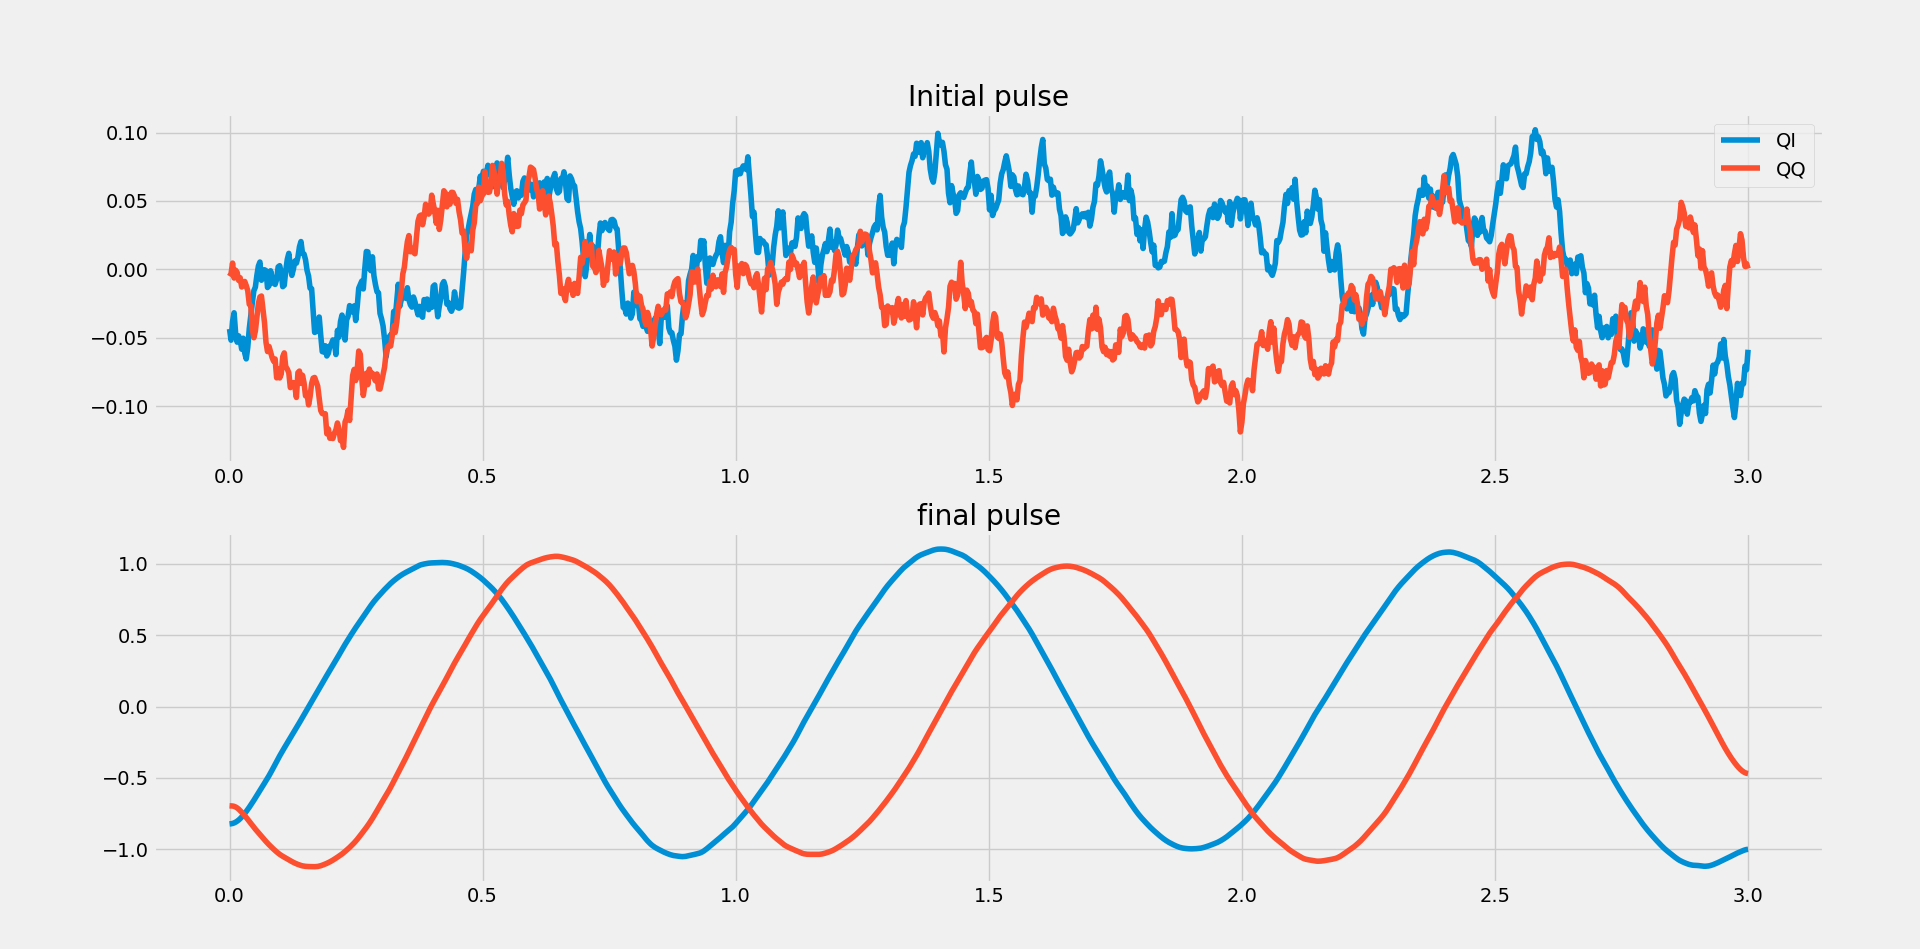
\includegraphics[width=1\columnwidth]{Results/qubit-band-amp-const/pulses.png}
%     \caption{Control pulses before and after GRAPE optimization with amplitude and bandwidth constraints}
%     \label{fig:band-amp-const-qubit}
% \end{figure}
\begin{figure}[H]
 \begin{center}
        %% Creator: Matplotlib, PGF backend
%%
%% To include the figure in your LaTeX document, write
%%   \input{<filename>.pgf}
%%
%% Make sure the required packages are loaded in your preamble
%%   \usepackage{pgf}
%%
%% and, on pdftex
%%   \usepackage[utf8]{inputenc}\DeclareUnicodeCharacter{2212}{-}
%%
%% or, on luatex and xetex
%%   \usepackage{unicode-math}
%%
%% Figures using additional raster images can only be included by \input if
%% they are in the same directory as the main LaTeX file. For loading figures
%% from other directories you can use the `import` package
%%   \usepackage{import}
%%
%% and then include the figures with
%%   \import{<path to file>}{<filename>.pgf}
%%
%% Matplotlib used the following preamble
%%
\begingroup%
\makeatletter%
\begin{pgfpicture}%
\pgfpathrectangle{\pgfpointorigin}{\pgfqpoint{4.650000in}{2.300000in}}%
\pgfusepath{use as bounding box, clip}%
\begin{pgfscope}%
\pgfsetbuttcap%
\pgfsetmiterjoin%
\definecolor{currentfill}{rgb}{1.000000,1.000000,1.000000}%
\pgfsetfillcolor{currentfill}%
\pgfsetlinewidth{0.000000pt}%
\definecolor{currentstroke}{rgb}{1.000000,1.000000,1.000000}%
\pgfsetstrokecolor{currentstroke}%
\pgfsetdash{}{0pt}%
\pgfpathmoveto{\pgfqpoint{0.000000in}{0.000000in}}%
\pgfpathlineto{\pgfqpoint{4.650000in}{0.000000in}}%
\pgfpathlineto{\pgfqpoint{4.650000in}{2.300000in}}%
\pgfpathlineto{\pgfqpoint{0.000000in}{2.300000in}}%
\pgfpathclose%
\pgfusepath{fill}%
\end{pgfscope}%
\begin{pgfscope}%
\pgfsetbuttcap%
\pgfsetmiterjoin%
\definecolor{currentfill}{rgb}{1.000000,1.000000,1.000000}%
\pgfsetfillcolor{currentfill}%
\pgfsetlinewidth{0.000000pt}%
\definecolor{currentstroke}{rgb}{0.000000,0.000000,0.000000}%
\pgfsetstrokecolor{currentstroke}%
\pgfsetstrokeopacity{0.000000}%
\pgfsetdash{}{0pt}%
\pgfpathmoveto{\pgfqpoint{0.602162in}{1.354089in}}%
\pgfpathlineto{\pgfqpoint{4.500000in}{1.354089in}}%
\pgfpathlineto{\pgfqpoint{4.500000in}{1.916667in}}%
\pgfpathlineto{\pgfqpoint{0.602162in}{1.916667in}}%
\pgfpathclose%
\pgfusepath{fill}%
\end{pgfscope}%
\begin{pgfscope}%
\pgfpathrectangle{\pgfqpoint{0.602162in}{1.354089in}}{\pgfqpoint{3.897838in}{0.562577in}}%
\pgfusepath{clip}%
\pgfsetrectcap%
\pgfsetroundjoin%
\pgfsetlinewidth{0.803000pt}%
\definecolor{currentstroke}{rgb}{0.501961,0.501961,0.501961}%
\pgfsetstrokecolor{currentstroke}%
\pgfsetstrokeopacity{0.200000}%
\pgfsetdash{}{0pt}%
\pgfpathmoveto{\pgfqpoint{0.779336in}{1.354089in}}%
\pgfpathlineto{\pgfqpoint{0.779336in}{1.916667in}}%
\pgfusepath{stroke}%
\end{pgfscope}%
\begin{pgfscope}%
\pgfsetbuttcap%
\pgfsetroundjoin%
\definecolor{currentfill}{rgb}{0.333333,0.333333,0.333333}%
\pgfsetfillcolor{currentfill}%
\pgfsetlinewidth{0.803000pt}%
\definecolor{currentstroke}{rgb}{0.333333,0.333333,0.333333}%
\pgfsetstrokecolor{currentstroke}%
\pgfsetdash{}{0pt}%
\pgfsys@defobject{currentmarker}{\pgfqpoint{0.000000in}{-0.048611in}}{\pgfqpoint{0.000000in}{0.000000in}}{%
\pgfpathmoveto{\pgfqpoint{0.000000in}{0.000000in}}%
\pgfpathlineto{\pgfqpoint{0.000000in}{-0.048611in}}%
\pgfusepath{stroke,fill}%
}%
\begin{pgfscope}%
\pgfsys@transformshift{0.779336in}{1.354089in}%
\pgfsys@useobject{currentmarker}{}%
\end{pgfscope}%
\end{pgfscope}%
\begin{pgfscope}%
\pgfpathrectangle{\pgfqpoint{0.602162in}{1.354089in}}{\pgfqpoint{3.897838in}{0.562577in}}%
\pgfusepath{clip}%
\pgfsetrectcap%
\pgfsetroundjoin%
\pgfsetlinewidth{0.803000pt}%
\definecolor{currentstroke}{rgb}{0.501961,0.501961,0.501961}%
\pgfsetstrokecolor{currentstroke}%
\pgfsetstrokeopacity{0.200000}%
\pgfsetdash{}{0pt}%
\pgfpathmoveto{\pgfqpoint{1.488034in}{1.354089in}}%
\pgfpathlineto{\pgfqpoint{1.488034in}{1.916667in}}%
\pgfusepath{stroke}%
\end{pgfscope}%
\begin{pgfscope}%
\pgfsetbuttcap%
\pgfsetroundjoin%
\definecolor{currentfill}{rgb}{0.333333,0.333333,0.333333}%
\pgfsetfillcolor{currentfill}%
\pgfsetlinewidth{0.803000pt}%
\definecolor{currentstroke}{rgb}{0.333333,0.333333,0.333333}%
\pgfsetstrokecolor{currentstroke}%
\pgfsetdash{}{0pt}%
\pgfsys@defobject{currentmarker}{\pgfqpoint{0.000000in}{-0.048611in}}{\pgfqpoint{0.000000in}{0.000000in}}{%
\pgfpathmoveto{\pgfqpoint{0.000000in}{0.000000in}}%
\pgfpathlineto{\pgfqpoint{0.000000in}{-0.048611in}}%
\pgfusepath{stroke,fill}%
}%
\begin{pgfscope}%
\pgfsys@transformshift{1.488034in}{1.354089in}%
\pgfsys@useobject{currentmarker}{}%
\end{pgfscope}%
\end{pgfscope}%
\begin{pgfscope}%
\pgfpathrectangle{\pgfqpoint{0.602162in}{1.354089in}}{\pgfqpoint{3.897838in}{0.562577in}}%
\pgfusepath{clip}%
\pgfsetrectcap%
\pgfsetroundjoin%
\pgfsetlinewidth{0.803000pt}%
\definecolor{currentstroke}{rgb}{0.501961,0.501961,0.501961}%
\pgfsetstrokecolor{currentstroke}%
\pgfsetstrokeopacity{0.200000}%
\pgfsetdash{}{0pt}%
\pgfpathmoveto{\pgfqpoint{2.196732in}{1.354089in}}%
\pgfpathlineto{\pgfqpoint{2.196732in}{1.916667in}}%
\pgfusepath{stroke}%
\end{pgfscope}%
\begin{pgfscope}%
\pgfsetbuttcap%
\pgfsetroundjoin%
\definecolor{currentfill}{rgb}{0.333333,0.333333,0.333333}%
\pgfsetfillcolor{currentfill}%
\pgfsetlinewidth{0.803000pt}%
\definecolor{currentstroke}{rgb}{0.333333,0.333333,0.333333}%
\pgfsetstrokecolor{currentstroke}%
\pgfsetdash{}{0pt}%
\pgfsys@defobject{currentmarker}{\pgfqpoint{0.000000in}{-0.048611in}}{\pgfqpoint{0.000000in}{0.000000in}}{%
\pgfpathmoveto{\pgfqpoint{0.000000in}{0.000000in}}%
\pgfpathlineto{\pgfqpoint{0.000000in}{-0.048611in}}%
\pgfusepath{stroke,fill}%
}%
\begin{pgfscope}%
\pgfsys@transformshift{2.196732in}{1.354089in}%
\pgfsys@useobject{currentmarker}{}%
\end{pgfscope}%
\end{pgfscope}%
\begin{pgfscope}%
\pgfpathrectangle{\pgfqpoint{0.602162in}{1.354089in}}{\pgfqpoint{3.897838in}{0.562577in}}%
\pgfusepath{clip}%
\pgfsetrectcap%
\pgfsetroundjoin%
\pgfsetlinewidth{0.803000pt}%
\definecolor{currentstroke}{rgb}{0.501961,0.501961,0.501961}%
\pgfsetstrokecolor{currentstroke}%
\pgfsetstrokeopacity{0.200000}%
\pgfsetdash{}{0pt}%
\pgfpathmoveto{\pgfqpoint{2.905430in}{1.354089in}}%
\pgfpathlineto{\pgfqpoint{2.905430in}{1.916667in}}%
\pgfusepath{stroke}%
\end{pgfscope}%
\begin{pgfscope}%
\pgfsetbuttcap%
\pgfsetroundjoin%
\definecolor{currentfill}{rgb}{0.333333,0.333333,0.333333}%
\pgfsetfillcolor{currentfill}%
\pgfsetlinewidth{0.803000pt}%
\definecolor{currentstroke}{rgb}{0.333333,0.333333,0.333333}%
\pgfsetstrokecolor{currentstroke}%
\pgfsetdash{}{0pt}%
\pgfsys@defobject{currentmarker}{\pgfqpoint{0.000000in}{-0.048611in}}{\pgfqpoint{0.000000in}{0.000000in}}{%
\pgfpathmoveto{\pgfqpoint{0.000000in}{0.000000in}}%
\pgfpathlineto{\pgfqpoint{0.000000in}{-0.048611in}}%
\pgfusepath{stroke,fill}%
}%
\begin{pgfscope}%
\pgfsys@transformshift{2.905430in}{1.354089in}%
\pgfsys@useobject{currentmarker}{}%
\end{pgfscope}%
\end{pgfscope}%
\begin{pgfscope}%
\pgfpathrectangle{\pgfqpoint{0.602162in}{1.354089in}}{\pgfqpoint{3.897838in}{0.562577in}}%
\pgfusepath{clip}%
\pgfsetrectcap%
\pgfsetroundjoin%
\pgfsetlinewidth{0.803000pt}%
\definecolor{currentstroke}{rgb}{0.501961,0.501961,0.501961}%
\pgfsetstrokecolor{currentstroke}%
\pgfsetstrokeopacity{0.200000}%
\pgfsetdash{}{0pt}%
\pgfpathmoveto{\pgfqpoint{3.614128in}{1.354089in}}%
\pgfpathlineto{\pgfqpoint{3.614128in}{1.916667in}}%
\pgfusepath{stroke}%
\end{pgfscope}%
\begin{pgfscope}%
\pgfsetbuttcap%
\pgfsetroundjoin%
\definecolor{currentfill}{rgb}{0.333333,0.333333,0.333333}%
\pgfsetfillcolor{currentfill}%
\pgfsetlinewidth{0.803000pt}%
\definecolor{currentstroke}{rgb}{0.333333,0.333333,0.333333}%
\pgfsetstrokecolor{currentstroke}%
\pgfsetdash{}{0pt}%
\pgfsys@defobject{currentmarker}{\pgfqpoint{0.000000in}{-0.048611in}}{\pgfqpoint{0.000000in}{0.000000in}}{%
\pgfpathmoveto{\pgfqpoint{0.000000in}{0.000000in}}%
\pgfpathlineto{\pgfqpoint{0.000000in}{-0.048611in}}%
\pgfusepath{stroke,fill}%
}%
\begin{pgfscope}%
\pgfsys@transformshift{3.614128in}{1.354089in}%
\pgfsys@useobject{currentmarker}{}%
\end{pgfscope}%
\end{pgfscope}%
\begin{pgfscope}%
\pgfpathrectangle{\pgfqpoint{0.602162in}{1.354089in}}{\pgfqpoint{3.897838in}{0.562577in}}%
\pgfusepath{clip}%
\pgfsetrectcap%
\pgfsetroundjoin%
\pgfsetlinewidth{0.803000pt}%
\definecolor{currentstroke}{rgb}{0.501961,0.501961,0.501961}%
\pgfsetstrokecolor{currentstroke}%
\pgfsetstrokeopacity{0.200000}%
\pgfsetdash{}{0pt}%
\pgfpathmoveto{\pgfqpoint{4.322826in}{1.354089in}}%
\pgfpathlineto{\pgfqpoint{4.322826in}{1.916667in}}%
\pgfusepath{stroke}%
\end{pgfscope}%
\begin{pgfscope}%
\pgfsetbuttcap%
\pgfsetroundjoin%
\definecolor{currentfill}{rgb}{0.333333,0.333333,0.333333}%
\pgfsetfillcolor{currentfill}%
\pgfsetlinewidth{0.803000pt}%
\definecolor{currentstroke}{rgb}{0.333333,0.333333,0.333333}%
\pgfsetstrokecolor{currentstroke}%
\pgfsetdash{}{0pt}%
\pgfsys@defobject{currentmarker}{\pgfqpoint{0.000000in}{-0.048611in}}{\pgfqpoint{0.000000in}{0.000000in}}{%
\pgfpathmoveto{\pgfqpoint{0.000000in}{0.000000in}}%
\pgfpathlineto{\pgfqpoint{0.000000in}{-0.048611in}}%
\pgfusepath{stroke,fill}%
}%
\begin{pgfscope}%
\pgfsys@transformshift{4.322826in}{1.354089in}%
\pgfsys@useobject{currentmarker}{}%
\end{pgfscope}%
\end{pgfscope}%
\begin{pgfscope}%
\pgfpathrectangle{\pgfqpoint{0.602162in}{1.354089in}}{\pgfqpoint{3.897838in}{0.562577in}}%
\pgfusepath{clip}%
\pgfsetrectcap%
\pgfsetroundjoin%
\pgfsetlinewidth{0.803000pt}%
\definecolor{currentstroke}{rgb}{0.501961,0.501961,0.501961}%
\pgfsetstrokecolor{currentstroke}%
\pgfsetstrokeopacity{0.200000}%
\pgfsetdash{}{0pt}%
\pgfpathmoveto{\pgfqpoint{0.602162in}{1.438285in}}%
\pgfpathlineto{\pgfqpoint{4.500000in}{1.438285in}}%
\pgfusepath{stroke}%
\end{pgfscope}%
\begin{pgfscope}%
\pgfsetbuttcap%
\pgfsetroundjoin%
\definecolor{currentfill}{rgb}{0.333333,0.333333,0.333333}%
\pgfsetfillcolor{currentfill}%
\pgfsetlinewidth{0.803000pt}%
\definecolor{currentstroke}{rgb}{0.333333,0.333333,0.333333}%
\pgfsetstrokecolor{currentstroke}%
\pgfsetdash{}{0pt}%
\pgfsys@defobject{currentmarker}{\pgfqpoint{-0.048611in}{0.000000in}}{\pgfqpoint{0.000000in}{0.000000in}}{%
\pgfpathmoveto{\pgfqpoint{0.000000in}{0.000000in}}%
\pgfpathlineto{\pgfqpoint{-0.048611in}{0.000000in}}%
\pgfusepath{stroke,fill}%
}%
\begin{pgfscope}%
\pgfsys@transformshift{0.602162in}{1.438285in}%
\pgfsys@useobject{currentmarker}{}%
\end{pgfscope}%
\end{pgfscope}%
\begin{pgfscope}%
\definecolor{textcolor}{rgb}{0.333333,0.333333,0.333333}%
\pgfsetstrokecolor{textcolor}%
\pgfsetfillcolor{textcolor}%
\pgftext[x=0.150000in, y=1.390059in, left, base]{\color{textcolor}\rmfamily\fontsize{10.000000}{12.000000}\selectfont \(\displaystyle {-0.05}\)}%
\end{pgfscope}%
\begin{pgfscope}%
\pgfpathrectangle{\pgfqpoint{0.602162in}{1.354089in}}{\pgfqpoint{3.897838in}{0.562577in}}%
\pgfusepath{clip}%
\pgfsetrectcap%
\pgfsetroundjoin%
\pgfsetlinewidth{0.803000pt}%
\definecolor{currentstroke}{rgb}{0.501961,0.501961,0.501961}%
\pgfsetstrokecolor{currentstroke}%
\pgfsetstrokeopacity{0.200000}%
\pgfsetdash{}{0pt}%
\pgfpathmoveto{\pgfqpoint{0.602162in}{1.636852in}}%
\pgfpathlineto{\pgfqpoint{4.500000in}{1.636852in}}%
\pgfusepath{stroke}%
\end{pgfscope}%
\begin{pgfscope}%
\pgfsetbuttcap%
\pgfsetroundjoin%
\definecolor{currentfill}{rgb}{0.333333,0.333333,0.333333}%
\pgfsetfillcolor{currentfill}%
\pgfsetlinewidth{0.803000pt}%
\definecolor{currentstroke}{rgb}{0.333333,0.333333,0.333333}%
\pgfsetstrokecolor{currentstroke}%
\pgfsetdash{}{0pt}%
\pgfsys@defobject{currentmarker}{\pgfqpoint{-0.048611in}{0.000000in}}{\pgfqpoint{0.000000in}{0.000000in}}{%
\pgfpathmoveto{\pgfqpoint{0.000000in}{0.000000in}}%
\pgfpathlineto{\pgfqpoint{-0.048611in}{0.000000in}}%
\pgfusepath{stroke,fill}%
}%
\begin{pgfscope}%
\pgfsys@transformshift{0.602162in}{1.636852in}%
\pgfsys@useobject{currentmarker}{}%
\end{pgfscope}%
\end{pgfscope}%
\begin{pgfscope}%
\definecolor{textcolor}{rgb}{0.333333,0.333333,0.333333}%
\pgfsetstrokecolor{textcolor}%
\pgfsetfillcolor{textcolor}%
\pgftext[x=0.258025in, y=1.588627in, left, base]{\color{textcolor}\rmfamily\fontsize{10.000000}{12.000000}\selectfont \(\displaystyle {0.00}\)}%
\end{pgfscope}%
\begin{pgfscope}%
\pgfpathrectangle{\pgfqpoint{0.602162in}{1.354089in}}{\pgfqpoint{3.897838in}{0.562577in}}%
\pgfusepath{clip}%
\pgfsetrectcap%
\pgfsetroundjoin%
\pgfsetlinewidth{0.803000pt}%
\definecolor{currentstroke}{rgb}{0.501961,0.501961,0.501961}%
\pgfsetstrokecolor{currentstroke}%
\pgfsetstrokeopacity{0.200000}%
\pgfsetdash{}{0pt}%
\pgfpathmoveto{\pgfqpoint{0.602162in}{1.835420in}}%
\pgfpathlineto{\pgfqpoint{4.500000in}{1.835420in}}%
\pgfusepath{stroke}%
\end{pgfscope}%
\begin{pgfscope}%
\pgfsetbuttcap%
\pgfsetroundjoin%
\definecolor{currentfill}{rgb}{0.333333,0.333333,0.333333}%
\pgfsetfillcolor{currentfill}%
\pgfsetlinewidth{0.803000pt}%
\definecolor{currentstroke}{rgb}{0.333333,0.333333,0.333333}%
\pgfsetstrokecolor{currentstroke}%
\pgfsetdash{}{0pt}%
\pgfsys@defobject{currentmarker}{\pgfqpoint{-0.048611in}{0.000000in}}{\pgfqpoint{0.000000in}{0.000000in}}{%
\pgfpathmoveto{\pgfqpoint{0.000000in}{0.000000in}}%
\pgfpathlineto{\pgfqpoint{-0.048611in}{0.000000in}}%
\pgfusepath{stroke,fill}%
}%
\begin{pgfscope}%
\pgfsys@transformshift{0.602162in}{1.835420in}%
\pgfsys@useobject{currentmarker}{}%
\end{pgfscope}%
\end{pgfscope}%
\begin{pgfscope}%
\definecolor{textcolor}{rgb}{0.333333,0.333333,0.333333}%
\pgfsetstrokecolor{textcolor}%
\pgfsetfillcolor{textcolor}%
\pgftext[x=0.258025in, y=1.787194in, left, base]{\color{textcolor}\rmfamily\fontsize{10.000000}{12.000000}\selectfont \(\displaystyle {0.05}\)}%
\end{pgfscope}%
\begin{pgfscope}%
\pgfpathrectangle{\pgfqpoint{0.602162in}{1.354089in}}{\pgfqpoint{3.897838in}{0.562577in}}%
\pgfusepath{clip}%
\pgfsetrectcap%
\pgfsetroundjoin%
\pgfsetlinewidth{1.505625pt}%
\definecolor{currentstroke}{rgb}{0.886275,0.290196,0.200000}%
\pgfsetstrokecolor{currentstroke}%
\pgfsetdash{}{0pt}%
\pgfpathmoveto{\pgfqpoint{0.779336in}{1.629627in}}%
\pgfpathlineto{\pgfqpoint{0.814949in}{1.629115in}}%
\pgfpathlineto{\pgfqpoint{0.886175in}{1.634130in}}%
\pgfpathlineto{\pgfqpoint{0.921788in}{1.632360in}}%
\pgfpathlineto{\pgfqpoint{0.939594in}{1.631741in}}%
\pgfpathlineto{\pgfqpoint{0.975207in}{1.633739in}}%
\pgfpathlineto{\pgfqpoint{0.993014in}{1.632665in}}%
\pgfpathlineto{\pgfqpoint{1.028627in}{1.635472in}}%
\pgfpathlineto{\pgfqpoint{1.099853in}{1.636567in}}%
\pgfpathlineto{\pgfqpoint{1.117659in}{1.635239in}}%
\pgfpathlineto{\pgfqpoint{1.153272in}{1.635010in}}%
\pgfpathlineto{\pgfqpoint{1.206692in}{1.632756in}}%
\pgfpathlineto{\pgfqpoint{1.260111in}{1.634339in}}%
\pgfpathlineto{\pgfqpoint{1.277917in}{1.633603in}}%
\pgfpathlineto{\pgfqpoint{1.295724in}{1.634773in}}%
\pgfpathlineto{\pgfqpoint{1.313530in}{1.633903in}}%
\pgfpathlineto{\pgfqpoint{1.331337in}{1.635679in}}%
\pgfpathlineto{\pgfqpoint{1.349143in}{1.634782in}}%
\pgfpathlineto{\pgfqpoint{1.384756in}{1.635310in}}%
\pgfpathlineto{\pgfqpoint{1.438176in}{1.631269in}}%
\pgfpathlineto{\pgfqpoint{1.491595in}{1.631715in}}%
\pgfpathlineto{\pgfqpoint{1.527208in}{1.633105in}}%
\pgfpathlineto{\pgfqpoint{1.580628in}{1.631884in}}%
\pgfpathlineto{\pgfqpoint{1.598434in}{1.631059in}}%
\pgfpathlineto{\pgfqpoint{1.616241in}{1.632452in}}%
\pgfpathlineto{\pgfqpoint{1.634047in}{1.631692in}}%
\pgfpathlineto{\pgfqpoint{1.651854in}{1.633318in}}%
\pgfpathlineto{\pgfqpoint{1.687466in}{1.633063in}}%
\pgfpathlineto{\pgfqpoint{1.705273in}{1.635453in}}%
\pgfpathlineto{\pgfqpoint{1.829918in}{1.637565in}}%
\pgfpathlineto{\pgfqpoint{1.865531in}{1.639239in}}%
\pgfpathlineto{\pgfqpoint{1.936757in}{1.639265in}}%
\pgfpathlineto{\pgfqpoint{1.972370in}{1.637223in}}%
\pgfpathlineto{\pgfqpoint{2.061403in}{1.638012in}}%
\pgfpathlineto{\pgfqpoint{2.079209in}{1.639272in}}%
\pgfpathlineto{\pgfqpoint{2.132628in}{1.636415in}}%
\pgfpathlineto{\pgfqpoint{2.186048in}{1.636682in}}%
\pgfpathlineto{\pgfqpoint{2.203854in}{1.635106in}}%
\pgfpathlineto{\pgfqpoint{2.239467in}{1.637092in}}%
\pgfpathlineto{\pgfqpoint{2.257274in}{1.635348in}}%
\pgfpathlineto{\pgfqpoint{2.346306in}{1.639779in}}%
\pgfpathlineto{\pgfqpoint{2.381919in}{1.642129in}}%
\pgfpathlineto{\pgfqpoint{2.435339in}{1.642252in}}%
\pgfpathlineto{\pgfqpoint{2.453145in}{1.643820in}}%
\pgfpathlineto{\pgfqpoint{2.524371in}{1.642561in}}%
\pgfpathlineto{\pgfqpoint{2.542178in}{1.643662in}}%
\pgfpathlineto{\pgfqpoint{2.577790in}{1.642575in}}%
\pgfpathlineto{\pgfqpoint{2.631210in}{1.643259in}}%
\pgfpathlineto{\pgfqpoint{2.684629in}{1.638278in}}%
\pgfpathlineto{\pgfqpoint{2.702436in}{1.638486in}}%
\pgfpathlineto{\pgfqpoint{2.738049in}{1.635662in}}%
\pgfpathlineto{\pgfqpoint{2.791468in}{1.636739in}}%
\pgfpathlineto{\pgfqpoint{2.809275in}{1.634642in}}%
\pgfpathlineto{\pgfqpoint{2.844888in}{1.634264in}}%
\pgfpathlineto{\pgfqpoint{2.880501in}{1.636233in}}%
\pgfpathlineto{\pgfqpoint{2.916114in}{1.633311in}}%
\pgfpathlineto{\pgfqpoint{3.076372in}{1.634625in}}%
\pgfpathlineto{\pgfqpoint{3.147598in}{1.631131in}}%
\pgfpathlineto{\pgfqpoint{3.201017in}{1.636397in}}%
\pgfpathlineto{\pgfqpoint{3.218824in}{1.634929in}}%
\pgfpathlineto{\pgfqpoint{3.236630in}{1.636334in}}%
\pgfpathlineto{\pgfqpoint{3.272243in}{1.634607in}}%
\pgfpathlineto{\pgfqpoint{3.290050in}{1.632968in}}%
\pgfpathlineto{\pgfqpoint{3.325663in}{1.633884in}}%
\pgfpathlineto{\pgfqpoint{3.361276in}{1.636050in}}%
\pgfpathlineto{\pgfqpoint{3.379082in}{1.634725in}}%
\pgfpathlineto{\pgfqpoint{3.396889in}{1.635354in}}%
\pgfpathlineto{\pgfqpoint{3.432502in}{1.633759in}}%
\pgfpathlineto{\pgfqpoint{3.450308in}{1.636030in}}%
\pgfpathlineto{\pgfqpoint{3.610566in}{1.638864in}}%
\pgfpathlineto{\pgfqpoint{3.646179in}{1.640636in}}%
\pgfpathlineto{\pgfqpoint{3.753018in}{1.640784in}}%
\pgfpathlineto{\pgfqpoint{3.788631in}{1.642461in}}%
\pgfpathlineto{\pgfqpoint{3.859857in}{1.643006in}}%
\pgfpathlineto{\pgfqpoint{3.895470in}{1.643941in}}%
\pgfpathlineto{\pgfqpoint{3.913276in}{1.641597in}}%
\pgfpathlineto{\pgfqpoint{3.931083in}{1.642752in}}%
\pgfpathlineto{\pgfqpoint{3.966696in}{1.639960in}}%
\pgfpathlineto{\pgfqpoint{4.037922in}{1.635924in}}%
\pgfpathlineto{\pgfqpoint{4.055728in}{1.636769in}}%
\pgfpathlineto{\pgfqpoint{4.073535in}{1.635278in}}%
\pgfpathlineto{\pgfqpoint{4.109148in}{1.636179in}}%
\pgfpathlineto{\pgfqpoint{4.144761in}{1.633576in}}%
\pgfpathlineto{\pgfqpoint{4.322826in}{1.628130in}}%
\pgfpathlineto{\pgfqpoint{4.322826in}{1.628130in}}%
\pgfusepath{stroke}%
\end{pgfscope}%
\begin{pgfscope}%
\pgfpathrectangle{\pgfqpoint{0.602162in}{1.354089in}}{\pgfqpoint{3.897838in}{0.562577in}}%
\pgfusepath{clip}%
\pgfsetrectcap%
\pgfsetroundjoin%
\pgfsetlinewidth{1.505625pt}%
\definecolor{currentstroke}{rgb}{0.203922,0.541176,0.741176}%
\pgfsetstrokecolor{currentstroke}%
\pgfsetdash{}{0pt}%
\pgfpathmoveto{\pgfqpoint{0.779336in}{1.641329in}}%
\pgfpathlineto{\pgfqpoint{0.814949in}{1.638734in}}%
\pgfpathlineto{\pgfqpoint{0.832755in}{1.639738in}}%
\pgfpathlineto{\pgfqpoint{0.868368in}{1.637183in}}%
\pgfpathlineto{\pgfqpoint{0.886175in}{1.636835in}}%
\pgfpathlineto{\pgfqpoint{0.921788in}{1.634048in}}%
\pgfpathlineto{\pgfqpoint{0.939594in}{1.635352in}}%
\pgfpathlineto{\pgfqpoint{0.993014in}{1.633374in}}%
\pgfpathlineto{\pgfqpoint{1.046433in}{1.631572in}}%
\pgfpathlineto{\pgfqpoint{1.064240in}{1.633111in}}%
\pgfpathlineto{\pgfqpoint{1.099853in}{1.629488in}}%
\pgfpathlineto{\pgfqpoint{1.135466in}{1.630157in}}%
\pgfpathlineto{\pgfqpoint{1.206692in}{1.630645in}}%
\pgfpathlineto{\pgfqpoint{1.242304in}{1.632166in}}%
\pgfpathlineto{\pgfqpoint{1.313530in}{1.632953in}}%
\pgfpathlineto{\pgfqpoint{1.331337in}{1.635041in}}%
\pgfpathlineto{\pgfqpoint{1.366950in}{1.634759in}}%
\pgfpathlineto{\pgfqpoint{1.402563in}{1.633770in}}%
\pgfpathlineto{\pgfqpoint{1.420369in}{1.632718in}}%
\pgfpathlineto{\pgfqpoint{1.455982in}{1.636591in}}%
\pgfpathlineto{\pgfqpoint{1.473789in}{1.636625in}}%
\pgfpathlineto{\pgfqpoint{1.509402in}{1.633777in}}%
\pgfpathlineto{\pgfqpoint{1.545015in}{1.635144in}}%
\pgfpathlineto{\pgfqpoint{1.562821in}{1.636739in}}%
\pgfpathlineto{\pgfqpoint{1.580628in}{1.634922in}}%
\pgfpathlineto{\pgfqpoint{1.616241in}{1.636065in}}%
\pgfpathlineto{\pgfqpoint{1.651854in}{1.639218in}}%
\pgfpathlineto{\pgfqpoint{1.669660in}{1.636921in}}%
\pgfpathlineto{\pgfqpoint{1.740886in}{1.635007in}}%
\pgfpathlineto{\pgfqpoint{1.776499in}{1.634928in}}%
\pgfpathlineto{\pgfqpoint{1.812112in}{1.634165in}}%
\pgfpathlineto{\pgfqpoint{1.883338in}{1.639648in}}%
\pgfpathlineto{\pgfqpoint{1.901144in}{1.638927in}}%
\pgfpathlineto{\pgfqpoint{1.936757in}{1.640639in}}%
\pgfpathlineto{\pgfqpoint{1.954564in}{1.638724in}}%
\pgfpathlineto{\pgfqpoint{1.972370in}{1.639698in}}%
\pgfpathlineto{\pgfqpoint{2.007983in}{1.637888in}}%
\pgfpathlineto{\pgfqpoint{2.061403in}{1.642299in}}%
\pgfpathlineto{\pgfqpoint{2.168241in}{1.638525in}}%
\pgfpathlineto{\pgfqpoint{2.221661in}{1.634090in}}%
\pgfpathlineto{\pgfqpoint{2.257274in}{1.635961in}}%
\pgfpathlineto{\pgfqpoint{2.292887in}{1.635283in}}%
\pgfpathlineto{\pgfqpoint{2.328500in}{1.634150in}}%
\pgfpathlineto{\pgfqpoint{2.435339in}{1.637982in}}%
\pgfpathlineto{\pgfqpoint{2.453145in}{1.636669in}}%
\pgfpathlineto{\pgfqpoint{2.470952in}{1.636925in}}%
\pgfpathlineto{\pgfqpoint{2.506565in}{1.635459in}}%
\pgfpathlineto{\pgfqpoint{2.542178in}{1.634907in}}%
\pgfpathlineto{\pgfqpoint{2.577790in}{1.637410in}}%
\pgfpathlineto{\pgfqpoint{2.631210in}{1.632243in}}%
\pgfpathlineto{\pgfqpoint{2.684629in}{1.631213in}}%
\pgfpathlineto{\pgfqpoint{2.791468in}{1.634625in}}%
\pgfpathlineto{\pgfqpoint{2.827081in}{1.634537in}}%
\pgfpathlineto{\pgfqpoint{2.862694in}{1.634927in}}%
\pgfpathlineto{\pgfqpoint{2.880501in}{1.634717in}}%
\pgfpathlineto{\pgfqpoint{2.898307in}{1.636399in}}%
\pgfpathlineto{\pgfqpoint{2.933920in}{1.636136in}}%
\pgfpathlineto{\pgfqpoint{2.969533in}{1.637651in}}%
\pgfpathlineto{\pgfqpoint{3.005146in}{1.638987in}}%
\pgfpathlineto{\pgfqpoint{3.076372in}{1.636443in}}%
\pgfpathlineto{\pgfqpoint{3.129791in}{1.638957in}}%
\pgfpathlineto{\pgfqpoint{3.183211in}{1.639381in}}%
\pgfpathlineto{\pgfqpoint{3.201017in}{1.640043in}}%
\pgfpathlineto{\pgfqpoint{3.236630in}{1.637732in}}%
\pgfpathlineto{\pgfqpoint{3.272243in}{1.639308in}}%
\pgfpathlineto{\pgfqpoint{3.290050in}{1.640486in}}%
\pgfpathlineto{\pgfqpoint{3.307856in}{1.638261in}}%
\pgfpathlineto{\pgfqpoint{3.361276in}{1.638381in}}%
\pgfpathlineto{\pgfqpoint{3.396889in}{1.637850in}}%
\pgfpathlineto{\pgfqpoint{3.414695in}{1.639688in}}%
\pgfpathlineto{\pgfqpoint{3.468114in}{1.638010in}}%
\pgfpathlineto{\pgfqpoint{3.485921in}{1.639345in}}%
\pgfpathlineto{\pgfqpoint{3.521534in}{1.638306in}}%
\pgfpathlineto{\pgfqpoint{3.539340in}{1.636064in}}%
\pgfpathlineto{\pgfqpoint{3.592760in}{1.638847in}}%
\pgfpathlineto{\pgfqpoint{3.717405in}{1.632134in}}%
\pgfpathlineto{\pgfqpoint{3.735212in}{1.634382in}}%
\pgfpathlineto{\pgfqpoint{3.770825in}{1.633867in}}%
\pgfpathlineto{\pgfqpoint{3.824244in}{1.637855in}}%
\pgfpathlineto{\pgfqpoint{3.913276in}{1.637792in}}%
\pgfpathlineto{\pgfqpoint{3.984502in}{1.636245in}}%
\pgfpathlineto{\pgfqpoint{4.020115in}{1.636612in}}%
\pgfpathlineto{\pgfqpoint{4.037922in}{1.637738in}}%
\pgfpathlineto{\pgfqpoint{4.091341in}{1.636212in}}%
\pgfpathlineto{\pgfqpoint{4.109148in}{1.638058in}}%
\pgfpathlineto{\pgfqpoint{4.180374in}{1.632756in}}%
\pgfpathlineto{\pgfqpoint{4.215987in}{1.633428in}}%
\pgfpathlineto{\pgfqpoint{4.269406in}{1.637366in}}%
\pgfpathlineto{\pgfqpoint{4.322826in}{1.641674in}}%
\pgfpathlineto{\pgfqpoint{4.322826in}{1.641674in}}%
\pgfusepath{stroke}%
\end{pgfscope}%
\begin{pgfscope}%
\pgfsetrectcap%
\pgfsetmiterjoin%
\pgfsetlinewidth{1.003750pt}%
\definecolor{currentstroke}{rgb}{1.000000,1.000000,1.000000}%
\pgfsetstrokecolor{currentstroke}%
\pgfsetdash{}{0pt}%
\pgfpathmoveto{\pgfqpoint{0.602162in}{1.354089in}}%
\pgfpathlineto{\pgfqpoint{0.602162in}{1.916667in}}%
\pgfusepath{stroke}%
\end{pgfscope}%
\begin{pgfscope}%
\pgfsetrectcap%
\pgfsetmiterjoin%
\pgfsetlinewidth{1.003750pt}%
\definecolor{currentstroke}{rgb}{1.000000,1.000000,1.000000}%
\pgfsetstrokecolor{currentstroke}%
\pgfsetdash{}{0pt}%
\pgfpathmoveto{\pgfqpoint{4.500000in}{1.354089in}}%
\pgfpathlineto{\pgfqpoint{4.500000in}{1.916667in}}%
\pgfusepath{stroke}%
\end{pgfscope}%
\begin{pgfscope}%
\pgfsetrectcap%
\pgfsetmiterjoin%
\pgfsetlinewidth{1.003750pt}%
\definecolor{currentstroke}{rgb}{1.000000,1.000000,1.000000}%
\pgfsetstrokecolor{currentstroke}%
\pgfsetdash{}{0pt}%
\pgfpathmoveto{\pgfqpoint{0.602162in}{1.354089in}}%
\pgfpathlineto{\pgfqpoint{4.500000in}{1.354089in}}%
\pgfusepath{stroke}%
\end{pgfscope}%
\begin{pgfscope}%
\pgfsetrectcap%
\pgfsetmiterjoin%
\pgfsetlinewidth{1.003750pt}%
\definecolor{currentstroke}{rgb}{1.000000,1.000000,1.000000}%
\pgfsetstrokecolor{currentstroke}%
\pgfsetdash{}{0pt}%
\pgfpathmoveto{\pgfqpoint{0.602162in}{1.916667in}}%
\pgfpathlineto{\pgfqpoint{4.500000in}{1.916667in}}%
\pgfusepath{stroke}%
\end{pgfscope}%
\begin{pgfscope}%
\definecolor{textcolor}{rgb}{0.000000,0.000000,0.000000}%
\pgfsetstrokecolor{textcolor}%
\pgfsetfillcolor{textcolor}%
\pgftext[x=2.551081in,y=2.000000in,,base]{\color{textcolor}\rmfamily\fontsize{14.000000}{16.800000}\selectfont Initial pulse (random)}%
\end{pgfscope}%
\begin{pgfscope}%
\pgfsetbuttcap%
\pgfsetmiterjoin%
\definecolor{currentfill}{rgb}{1.000000,1.000000,1.000000}%
\pgfsetfillcolor{currentfill}%
\pgfsetfillopacity{0.800000}%
\pgfsetlinewidth{0.501875pt}%
\definecolor{currentstroke}{rgb}{0.800000,0.800000,0.800000}%
\pgfsetstrokecolor{currentstroke}%
\pgfsetstrokeopacity{0.800000}%
\pgfsetdash{}{0pt}%
\pgfpathmoveto{\pgfqpoint{3.090221in}{1.691636in}}%
\pgfpathlineto{\pgfqpoint{4.472222in}{1.691636in}}%
\pgfpathquadraticcurveto{\pgfqpoint{4.500000in}{1.691636in}}{\pgfqpoint{4.500000in}{1.719414in}}%
\pgfpathlineto{\pgfqpoint{4.500000in}{1.911929in}}%
\pgfpathquadraticcurveto{\pgfqpoint{4.500000in}{1.939706in}}{\pgfqpoint{4.472222in}{1.939706in}}%
\pgfpathlineto{\pgfqpoint{3.090221in}{1.939706in}}%
\pgfpathquadraticcurveto{\pgfqpoint{3.062444in}{1.939706in}}{\pgfqpoint{3.062444in}{1.911929in}}%
\pgfpathlineto{\pgfqpoint{3.062444in}{1.719414in}}%
\pgfpathquadraticcurveto{\pgfqpoint{3.062444in}{1.691636in}}{\pgfqpoint{3.090221in}{1.691636in}}%
\pgfpathclose%
\pgfusepath{stroke,fill}%
\end{pgfscope}%
\begin{pgfscope}%
\pgfsetrectcap%
\pgfsetroundjoin%
\pgfsetlinewidth{1.505625pt}%
\definecolor{currentstroke}{rgb}{0.886275,0.290196,0.200000}%
\pgfsetstrokecolor{currentstroke}%
\pgfsetdash{}{0pt}%
\pgfpathmoveto{\pgfqpoint{3.117999in}{1.835540in}}%
\pgfpathlineto{\pgfqpoint{3.395777in}{1.835540in}}%
\pgfusepath{stroke}%
\end{pgfscope}%
\begin{pgfscope}%
\definecolor{textcolor}{rgb}{0.000000,0.000000,0.000000}%
\pgfsetstrokecolor{textcolor}%
\pgfsetfillcolor{textcolor}%
\pgftext[x=3.506888in,y=1.786929in,left,base]{\color{textcolor}\rmfamily\fontsize{10.000000}{12.000000}\selectfont \(\displaystyle \epsilon_I\)}%
\end{pgfscope}%
\begin{pgfscope}%
\pgfsetrectcap%
\pgfsetroundjoin%
\pgfsetlinewidth{1.505625pt}%
\definecolor{currentstroke}{rgb}{0.203922,0.541176,0.741176}%
\pgfsetstrokecolor{currentstroke}%
\pgfsetdash{}{0pt}%
\pgfpathmoveto{\pgfqpoint{3.904767in}{1.835540in}}%
\pgfpathlineto{\pgfqpoint{4.182544in}{1.835540in}}%
\pgfusepath{stroke}%
\end{pgfscope}%
\begin{pgfscope}%
\definecolor{textcolor}{rgb}{0.000000,0.000000,0.000000}%
\pgfsetstrokecolor{textcolor}%
\pgfsetfillcolor{textcolor}%
\pgftext[x=4.293655in,y=1.786929in,left,base]{\color{textcolor}\rmfamily\fontsize{10.000000}{12.000000}\selectfont \(\displaystyle \epsilon_Q\)}%
\end{pgfscope}%
\begin{pgfscope}%
\pgfsetbuttcap%
\pgfsetmiterjoin%
\definecolor{currentfill}{rgb}{1.000000,1.000000,1.000000}%
\pgfsetfillcolor{currentfill}%
\pgfsetlinewidth{0.000000pt}%
\definecolor{currentstroke}{rgb}{0.000000,0.000000,0.000000}%
\pgfsetstrokecolor{currentstroke}%
\pgfsetstrokeopacity{0.000000}%
\pgfsetdash{}{0pt}%
\pgfpathmoveto{\pgfqpoint{0.602162in}{0.370679in}}%
\pgfpathlineto{\pgfqpoint{4.500000in}{0.370679in}}%
\pgfpathlineto{\pgfqpoint{4.500000in}{0.933256in}}%
\pgfpathlineto{\pgfqpoint{0.602162in}{0.933256in}}%
\pgfpathclose%
\pgfusepath{fill}%
\end{pgfscope}%
\begin{pgfscope}%
\pgfpathrectangle{\pgfqpoint{0.602162in}{0.370679in}}{\pgfqpoint{3.897838in}{0.562577in}}%
\pgfusepath{clip}%
\pgfsetrectcap%
\pgfsetroundjoin%
\pgfsetlinewidth{0.803000pt}%
\definecolor{currentstroke}{rgb}{0.501961,0.501961,0.501961}%
\pgfsetstrokecolor{currentstroke}%
\pgfsetstrokeopacity{0.200000}%
\pgfsetdash{}{0pt}%
\pgfpathmoveto{\pgfqpoint{0.779336in}{0.370679in}}%
\pgfpathlineto{\pgfqpoint{0.779336in}{0.933256in}}%
\pgfusepath{stroke}%
\end{pgfscope}%
\begin{pgfscope}%
\pgfsetbuttcap%
\pgfsetroundjoin%
\definecolor{currentfill}{rgb}{0.333333,0.333333,0.333333}%
\pgfsetfillcolor{currentfill}%
\pgfsetlinewidth{0.803000pt}%
\definecolor{currentstroke}{rgb}{0.333333,0.333333,0.333333}%
\pgfsetstrokecolor{currentstroke}%
\pgfsetdash{}{0pt}%
\pgfsys@defobject{currentmarker}{\pgfqpoint{0.000000in}{-0.048611in}}{\pgfqpoint{0.000000in}{0.000000in}}{%
\pgfpathmoveto{\pgfqpoint{0.000000in}{0.000000in}}%
\pgfpathlineto{\pgfqpoint{0.000000in}{-0.048611in}}%
\pgfusepath{stroke,fill}%
}%
\begin{pgfscope}%
\pgfsys@transformshift{0.779336in}{0.370679in}%
\pgfsys@useobject{currentmarker}{}%
\end{pgfscope}%
\end{pgfscope}%
\begin{pgfscope}%
\definecolor{textcolor}{rgb}{0.333333,0.333333,0.333333}%
\pgfsetstrokecolor{textcolor}%
\pgfsetfillcolor{textcolor}%
\pgftext[x=0.779336in,y=0.273457in,,top]{\color{textcolor}\rmfamily\fontsize{10.000000}{12.000000}\selectfont \(\displaystyle {0}\)}%
\end{pgfscope}%
\begin{pgfscope}%
\pgfpathrectangle{\pgfqpoint{0.602162in}{0.370679in}}{\pgfqpoint{3.897838in}{0.562577in}}%
\pgfusepath{clip}%
\pgfsetrectcap%
\pgfsetroundjoin%
\pgfsetlinewidth{0.803000pt}%
\definecolor{currentstroke}{rgb}{0.501961,0.501961,0.501961}%
\pgfsetstrokecolor{currentstroke}%
\pgfsetstrokeopacity{0.200000}%
\pgfsetdash{}{0pt}%
\pgfpathmoveto{\pgfqpoint{1.488034in}{0.370679in}}%
\pgfpathlineto{\pgfqpoint{1.488034in}{0.933256in}}%
\pgfusepath{stroke}%
\end{pgfscope}%
\begin{pgfscope}%
\pgfsetbuttcap%
\pgfsetroundjoin%
\definecolor{currentfill}{rgb}{0.333333,0.333333,0.333333}%
\pgfsetfillcolor{currentfill}%
\pgfsetlinewidth{0.803000pt}%
\definecolor{currentstroke}{rgb}{0.333333,0.333333,0.333333}%
\pgfsetstrokecolor{currentstroke}%
\pgfsetdash{}{0pt}%
\pgfsys@defobject{currentmarker}{\pgfqpoint{0.000000in}{-0.048611in}}{\pgfqpoint{0.000000in}{0.000000in}}{%
\pgfpathmoveto{\pgfqpoint{0.000000in}{0.000000in}}%
\pgfpathlineto{\pgfqpoint{0.000000in}{-0.048611in}}%
\pgfusepath{stroke,fill}%
}%
\begin{pgfscope}%
\pgfsys@transformshift{1.488034in}{0.370679in}%
\pgfsys@useobject{currentmarker}{}%
\end{pgfscope}%
\end{pgfscope}%
\begin{pgfscope}%
\definecolor{textcolor}{rgb}{0.333333,0.333333,0.333333}%
\pgfsetstrokecolor{textcolor}%
\pgfsetfillcolor{textcolor}%
\pgftext[x=1.488034in,y=0.273457in,,top]{\color{textcolor}\rmfamily\fontsize{10.000000}{12.000000}\selectfont \(\displaystyle {5}\)}%
\end{pgfscope}%
\begin{pgfscope}%
\pgfpathrectangle{\pgfqpoint{0.602162in}{0.370679in}}{\pgfqpoint{3.897838in}{0.562577in}}%
\pgfusepath{clip}%
\pgfsetrectcap%
\pgfsetroundjoin%
\pgfsetlinewidth{0.803000pt}%
\definecolor{currentstroke}{rgb}{0.501961,0.501961,0.501961}%
\pgfsetstrokecolor{currentstroke}%
\pgfsetstrokeopacity{0.200000}%
\pgfsetdash{}{0pt}%
\pgfpathmoveto{\pgfqpoint{2.196732in}{0.370679in}}%
\pgfpathlineto{\pgfqpoint{2.196732in}{0.933256in}}%
\pgfusepath{stroke}%
\end{pgfscope}%
\begin{pgfscope}%
\pgfsetbuttcap%
\pgfsetroundjoin%
\definecolor{currentfill}{rgb}{0.333333,0.333333,0.333333}%
\pgfsetfillcolor{currentfill}%
\pgfsetlinewidth{0.803000pt}%
\definecolor{currentstroke}{rgb}{0.333333,0.333333,0.333333}%
\pgfsetstrokecolor{currentstroke}%
\pgfsetdash{}{0pt}%
\pgfsys@defobject{currentmarker}{\pgfqpoint{0.000000in}{-0.048611in}}{\pgfqpoint{0.000000in}{0.000000in}}{%
\pgfpathmoveto{\pgfqpoint{0.000000in}{0.000000in}}%
\pgfpathlineto{\pgfqpoint{0.000000in}{-0.048611in}}%
\pgfusepath{stroke,fill}%
}%
\begin{pgfscope}%
\pgfsys@transformshift{2.196732in}{0.370679in}%
\pgfsys@useobject{currentmarker}{}%
\end{pgfscope}%
\end{pgfscope}%
\begin{pgfscope}%
\definecolor{textcolor}{rgb}{0.333333,0.333333,0.333333}%
\pgfsetstrokecolor{textcolor}%
\pgfsetfillcolor{textcolor}%
\pgftext[x=2.196732in,y=0.273457in,,top]{\color{textcolor}\rmfamily\fontsize{10.000000}{12.000000}\selectfont \(\displaystyle {10}\)}%
\end{pgfscope}%
\begin{pgfscope}%
\pgfpathrectangle{\pgfqpoint{0.602162in}{0.370679in}}{\pgfqpoint{3.897838in}{0.562577in}}%
\pgfusepath{clip}%
\pgfsetrectcap%
\pgfsetroundjoin%
\pgfsetlinewidth{0.803000pt}%
\definecolor{currentstroke}{rgb}{0.501961,0.501961,0.501961}%
\pgfsetstrokecolor{currentstroke}%
\pgfsetstrokeopacity{0.200000}%
\pgfsetdash{}{0pt}%
\pgfpathmoveto{\pgfqpoint{2.905430in}{0.370679in}}%
\pgfpathlineto{\pgfqpoint{2.905430in}{0.933256in}}%
\pgfusepath{stroke}%
\end{pgfscope}%
\begin{pgfscope}%
\pgfsetbuttcap%
\pgfsetroundjoin%
\definecolor{currentfill}{rgb}{0.333333,0.333333,0.333333}%
\pgfsetfillcolor{currentfill}%
\pgfsetlinewidth{0.803000pt}%
\definecolor{currentstroke}{rgb}{0.333333,0.333333,0.333333}%
\pgfsetstrokecolor{currentstroke}%
\pgfsetdash{}{0pt}%
\pgfsys@defobject{currentmarker}{\pgfqpoint{0.000000in}{-0.048611in}}{\pgfqpoint{0.000000in}{0.000000in}}{%
\pgfpathmoveto{\pgfqpoint{0.000000in}{0.000000in}}%
\pgfpathlineto{\pgfqpoint{0.000000in}{-0.048611in}}%
\pgfusepath{stroke,fill}%
}%
\begin{pgfscope}%
\pgfsys@transformshift{2.905430in}{0.370679in}%
\pgfsys@useobject{currentmarker}{}%
\end{pgfscope}%
\end{pgfscope}%
\begin{pgfscope}%
\definecolor{textcolor}{rgb}{0.333333,0.333333,0.333333}%
\pgfsetstrokecolor{textcolor}%
\pgfsetfillcolor{textcolor}%
\pgftext[x=2.905430in,y=0.273457in,,top]{\color{textcolor}\rmfamily\fontsize{10.000000}{12.000000}\selectfont \(\displaystyle {15}\)}%
\end{pgfscope}%
\begin{pgfscope}%
\pgfpathrectangle{\pgfqpoint{0.602162in}{0.370679in}}{\pgfqpoint{3.897838in}{0.562577in}}%
\pgfusepath{clip}%
\pgfsetrectcap%
\pgfsetroundjoin%
\pgfsetlinewidth{0.803000pt}%
\definecolor{currentstroke}{rgb}{0.501961,0.501961,0.501961}%
\pgfsetstrokecolor{currentstroke}%
\pgfsetstrokeopacity{0.200000}%
\pgfsetdash{}{0pt}%
\pgfpathmoveto{\pgfqpoint{3.614128in}{0.370679in}}%
\pgfpathlineto{\pgfqpoint{3.614128in}{0.933256in}}%
\pgfusepath{stroke}%
\end{pgfscope}%
\begin{pgfscope}%
\pgfsetbuttcap%
\pgfsetroundjoin%
\definecolor{currentfill}{rgb}{0.333333,0.333333,0.333333}%
\pgfsetfillcolor{currentfill}%
\pgfsetlinewidth{0.803000pt}%
\definecolor{currentstroke}{rgb}{0.333333,0.333333,0.333333}%
\pgfsetstrokecolor{currentstroke}%
\pgfsetdash{}{0pt}%
\pgfsys@defobject{currentmarker}{\pgfqpoint{0.000000in}{-0.048611in}}{\pgfqpoint{0.000000in}{0.000000in}}{%
\pgfpathmoveto{\pgfqpoint{0.000000in}{0.000000in}}%
\pgfpathlineto{\pgfqpoint{0.000000in}{-0.048611in}}%
\pgfusepath{stroke,fill}%
}%
\begin{pgfscope}%
\pgfsys@transformshift{3.614128in}{0.370679in}%
\pgfsys@useobject{currentmarker}{}%
\end{pgfscope}%
\end{pgfscope}%
\begin{pgfscope}%
\definecolor{textcolor}{rgb}{0.333333,0.333333,0.333333}%
\pgfsetstrokecolor{textcolor}%
\pgfsetfillcolor{textcolor}%
\pgftext[x=3.614128in,y=0.273457in,,top]{\color{textcolor}\rmfamily\fontsize{10.000000}{12.000000}\selectfont \(\displaystyle {20}\)}%
\end{pgfscope}%
\begin{pgfscope}%
\pgfpathrectangle{\pgfqpoint{0.602162in}{0.370679in}}{\pgfqpoint{3.897838in}{0.562577in}}%
\pgfusepath{clip}%
\pgfsetrectcap%
\pgfsetroundjoin%
\pgfsetlinewidth{0.803000pt}%
\definecolor{currentstroke}{rgb}{0.501961,0.501961,0.501961}%
\pgfsetstrokecolor{currentstroke}%
\pgfsetstrokeopacity{0.200000}%
\pgfsetdash{}{0pt}%
\pgfpathmoveto{\pgfqpoint{4.322826in}{0.370679in}}%
\pgfpathlineto{\pgfqpoint{4.322826in}{0.933256in}}%
\pgfusepath{stroke}%
\end{pgfscope}%
\begin{pgfscope}%
\pgfsetbuttcap%
\pgfsetroundjoin%
\definecolor{currentfill}{rgb}{0.333333,0.333333,0.333333}%
\pgfsetfillcolor{currentfill}%
\pgfsetlinewidth{0.803000pt}%
\definecolor{currentstroke}{rgb}{0.333333,0.333333,0.333333}%
\pgfsetstrokecolor{currentstroke}%
\pgfsetdash{}{0pt}%
\pgfsys@defobject{currentmarker}{\pgfqpoint{0.000000in}{-0.048611in}}{\pgfqpoint{0.000000in}{0.000000in}}{%
\pgfpathmoveto{\pgfqpoint{0.000000in}{0.000000in}}%
\pgfpathlineto{\pgfqpoint{0.000000in}{-0.048611in}}%
\pgfusepath{stroke,fill}%
}%
\begin{pgfscope}%
\pgfsys@transformshift{4.322826in}{0.370679in}%
\pgfsys@useobject{currentmarker}{}%
\end{pgfscope}%
\end{pgfscope}%
\begin{pgfscope}%
\definecolor{textcolor}{rgb}{0.333333,0.333333,0.333333}%
\pgfsetstrokecolor{textcolor}%
\pgfsetfillcolor{textcolor}%
\pgftext[x=4.322826in,y=0.273457in,,top]{\color{textcolor}\rmfamily\fontsize{10.000000}{12.000000}\selectfont \(\displaystyle {25}\)}%
\end{pgfscope}%
\begin{pgfscope}%
\pgfpathrectangle{\pgfqpoint{0.602162in}{0.370679in}}{\pgfqpoint{3.897838in}{0.562577in}}%
\pgfusepath{clip}%
\pgfsetrectcap%
\pgfsetroundjoin%
\pgfsetlinewidth{0.803000pt}%
\definecolor{currentstroke}{rgb}{0.501961,0.501961,0.501961}%
\pgfsetstrokecolor{currentstroke}%
\pgfsetstrokeopacity{0.200000}%
\pgfsetdash{}{0pt}%
\pgfpathmoveto{\pgfqpoint{0.602162in}{0.454874in}}%
\pgfpathlineto{\pgfqpoint{4.500000in}{0.454874in}}%
\pgfusepath{stroke}%
\end{pgfscope}%
\begin{pgfscope}%
\pgfsetbuttcap%
\pgfsetroundjoin%
\definecolor{currentfill}{rgb}{0.333333,0.333333,0.333333}%
\pgfsetfillcolor{currentfill}%
\pgfsetlinewidth{0.803000pt}%
\definecolor{currentstroke}{rgb}{0.333333,0.333333,0.333333}%
\pgfsetstrokecolor{currentstroke}%
\pgfsetdash{}{0pt}%
\pgfsys@defobject{currentmarker}{\pgfqpoint{-0.048611in}{0.000000in}}{\pgfqpoint{0.000000in}{0.000000in}}{%
\pgfpathmoveto{\pgfqpoint{0.000000in}{0.000000in}}%
\pgfpathlineto{\pgfqpoint{-0.048611in}{0.000000in}}%
\pgfusepath{stroke,fill}%
}%
\begin{pgfscope}%
\pgfsys@transformshift{0.602162in}{0.454874in}%
\pgfsys@useobject{currentmarker}{}%
\end{pgfscope}%
\end{pgfscope}%
\begin{pgfscope}%
\definecolor{textcolor}{rgb}{0.333333,0.333333,0.333333}%
\pgfsetstrokecolor{textcolor}%
\pgfsetfillcolor{textcolor}%
\pgftext[x=0.150000in, y=0.406649in, left, base]{\color{textcolor}\rmfamily\fontsize{10.000000}{12.000000}\selectfont \(\displaystyle {-0.05}\)}%
\end{pgfscope}%
\begin{pgfscope}%
\pgfpathrectangle{\pgfqpoint{0.602162in}{0.370679in}}{\pgfqpoint{3.897838in}{0.562577in}}%
\pgfusepath{clip}%
\pgfsetrectcap%
\pgfsetroundjoin%
\pgfsetlinewidth{0.803000pt}%
\definecolor{currentstroke}{rgb}{0.501961,0.501961,0.501961}%
\pgfsetstrokecolor{currentstroke}%
\pgfsetstrokeopacity{0.200000}%
\pgfsetdash{}{0pt}%
\pgfpathmoveto{\pgfqpoint{0.602162in}{0.653442in}}%
\pgfpathlineto{\pgfqpoint{4.500000in}{0.653442in}}%
\pgfusepath{stroke}%
\end{pgfscope}%
\begin{pgfscope}%
\pgfsetbuttcap%
\pgfsetroundjoin%
\definecolor{currentfill}{rgb}{0.333333,0.333333,0.333333}%
\pgfsetfillcolor{currentfill}%
\pgfsetlinewidth{0.803000pt}%
\definecolor{currentstroke}{rgb}{0.333333,0.333333,0.333333}%
\pgfsetstrokecolor{currentstroke}%
\pgfsetdash{}{0pt}%
\pgfsys@defobject{currentmarker}{\pgfqpoint{-0.048611in}{0.000000in}}{\pgfqpoint{0.000000in}{0.000000in}}{%
\pgfpathmoveto{\pgfqpoint{0.000000in}{0.000000in}}%
\pgfpathlineto{\pgfqpoint{-0.048611in}{0.000000in}}%
\pgfusepath{stroke,fill}%
}%
\begin{pgfscope}%
\pgfsys@transformshift{0.602162in}{0.653442in}%
\pgfsys@useobject{currentmarker}{}%
\end{pgfscope}%
\end{pgfscope}%
\begin{pgfscope}%
\definecolor{textcolor}{rgb}{0.333333,0.333333,0.333333}%
\pgfsetstrokecolor{textcolor}%
\pgfsetfillcolor{textcolor}%
\pgftext[x=0.258025in, y=0.605216in, left, base]{\color{textcolor}\rmfamily\fontsize{10.000000}{12.000000}\selectfont \(\displaystyle {0.00}\)}%
\end{pgfscope}%
\begin{pgfscope}%
\pgfpathrectangle{\pgfqpoint{0.602162in}{0.370679in}}{\pgfqpoint{3.897838in}{0.562577in}}%
\pgfusepath{clip}%
\pgfsetrectcap%
\pgfsetroundjoin%
\pgfsetlinewidth{0.803000pt}%
\definecolor{currentstroke}{rgb}{0.501961,0.501961,0.501961}%
\pgfsetstrokecolor{currentstroke}%
\pgfsetstrokeopacity{0.200000}%
\pgfsetdash{}{0pt}%
\pgfpathmoveto{\pgfqpoint{0.602162in}{0.852009in}}%
\pgfpathlineto{\pgfqpoint{4.500000in}{0.852009in}}%
\pgfusepath{stroke}%
\end{pgfscope}%
\begin{pgfscope}%
\pgfsetbuttcap%
\pgfsetroundjoin%
\definecolor{currentfill}{rgb}{0.333333,0.333333,0.333333}%
\pgfsetfillcolor{currentfill}%
\pgfsetlinewidth{0.803000pt}%
\definecolor{currentstroke}{rgb}{0.333333,0.333333,0.333333}%
\pgfsetstrokecolor{currentstroke}%
\pgfsetdash{}{0pt}%
\pgfsys@defobject{currentmarker}{\pgfqpoint{-0.048611in}{0.000000in}}{\pgfqpoint{0.000000in}{0.000000in}}{%
\pgfpathmoveto{\pgfqpoint{0.000000in}{0.000000in}}%
\pgfpathlineto{\pgfqpoint{-0.048611in}{0.000000in}}%
\pgfusepath{stroke,fill}%
}%
\begin{pgfscope}%
\pgfsys@transformshift{0.602162in}{0.852009in}%
\pgfsys@useobject{currentmarker}{}%
\end{pgfscope}%
\end{pgfscope}%
\begin{pgfscope}%
\definecolor{textcolor}{rgb}{0.333333,0.333333,0.333333}%
\pgfsetstrokecolor{textcolor}%
\pgfsetfillcolor{textcolor}%
\pgftext[x=0.258025in, y=0.803784in, left, base]{\color{textcolor}\rmfamily\fontsize{10.000000}{12.000000}\selectfont \(\displaystyle {0.05}\)}%
\end{pgfscope}%
\begin{pgfscope}%
\pgfpathrectangle{\pgfqpoint{0.602162in}{0.370679in}}{\pgfqpoint{3.897838in}{0.562577in}}%
\pgfusepath{clip}%
\pgfsetrectcap%
\pgfsetroundjoin%
\pgfsetlinewidth{1.505625pt}%
\definecolor{currentstroke}{rgb}{0.886275,0.290196,0.200000}%
\pgfsetstrokecolor{currentstroke}%
\pgfsetdash{}{0pt}%
\pgfpathmoveto{\pgfqpoint{0.779336in}{0.462904in}}%
\pgfpathlineto{\pgfqpoint{0.797142in}{0.485971in}}%
\pgfpathlineto{\pgfqpoint{0.832755in}{0.538118in}}%
\pgfpathlineto{\pgfqpoint{0.868368in}{0.599228in}}%
\pgfpathlineto{\pgfqpoint{0.921788in}{0.691887in}}%
\pgfpathlineto{\pgfqpoint{0.939594in}{0.724198in}}%
\pgfpathlineto{\pgfqpoint{0.993014in}{0.807973in}}%
\pgfpathlineto{\pgfqpoint{1.028627in}{0.850393in}}%
\pgfpathlineto{\pgfqpoint{1.064240in}{0.883600in}}%
\pgfpathlineto{\pgfqpoint{1.099853in}{0.898056in}}%
\pgfpathlineto{\pgfqpoint{1.117659in}{0.902511in}}%
\pgfpathlineto{\pgfqpoint{1.153272in}{0.893636in}}%
\pgfpathlineto{\pgfqpoint{1.171079in}{0.884879in}}%
\pgfpathlineto{\pgfqpoint{1.206692in}{0.856364in}}%
\pgfpathlineto{\pgfqpoint{1.242304in}{0.813789in}}%
\pgfpathlineto{\pgfqpoint{1.277917in}{0.764228in}}%
\pgfpathlineto{\pgfqpoint{1.295724in}{0.732658in}}%
\pgfpathlineto{\pgfqpoint{1.313530in}{0.706841in}}%
\pgfpathlineto{\pgfqpoint{1.331337in}{0.672287in}}%
\pgfpathlineto{\pgfqpoint{1.349143in}{0.644825in}}%
\pgfpathlineto{\pgfqpoint{1.384756in}{0.581001in}}%
\pgfpathlineto{\pgfqpoint{1.438176in}{0.497026in}}%
\pgfpathlineto{\pgfqpoint{1.473789in}{0.451348in}}%
\pgfpathlineto{\pgfqpoint{1.509402in}{0.420203in}}%
\pgfpathlineto{\pgfqpoint{1.527208in}{0.410940in}}%
\pgfpathlineto{\pgfqpoint{1.562821in}{0.398820in}}%
\pgfpathlineto{\pgfqpoint{1.580628in}{0.401614in}}%
\pgfpathlineto{\pgfqpoint{1.616241in}{0.411856in}}%
\pgfpathlineto{\pgfqpoint{1.634047in}{0.427962in}}%
\pgfpathlineto{\pgfqpoint{1.651854in}{0.440032in}}%
\pgfpathlineto{\pgfqpoint{1.705273in}{0.507269in}}%
\pgfpathlineto{\pgfqpoint{1.740886in}{0.564915in}}%
\pgfpathlineto{\pgfqpoint{1.794305in}{0.655998in}}%
\pgfpathlineto{\pgfqpoint{1.812112in}{0.689705in}}%
\pgfpathlineto{\pgfqpoint{1.883338in}{0.805894in}}%
\pgfpathlineto{\pgfqpoint{1.901144in}{0.826339in}}%
\pgfpathlineto{\pgfqpoint{1.918951in}{0.851455in}}%
\pgfpathlineto{\pgfqpoint{1.936757in}{0.865147in}}%
\pgfpathlineto{\pgfqpoint{1.954564in}{0.881641in}}%
\pgfpathlineto{\pgfqpoint{1.972370in}{0.891833in}}%
\pgfpathlineto{\pgfqpoint{1.990177in}{0.897205in}}%
\pgfpathlineto{\pgfqpoint{2.007983in}{0.904206in}}%
\pgfpathlineto{\pgfqpoint{2.043596in}{0.898569in}}%
\pgfpathlineto{\pgfqpoint{2.061403in}{0.891983in}}%
\pgfpathlineto{\pgfqpoint{2.097016in}{0.865844in}}%
\pgfpathlineto{\pgfqpoint{2.114822in}{0.843935in}}%
\pgfpathlineto{\pgfqpoint{2.132628in}{0.825113in}}%
\pgfpathlineto{\pgfqpoint{2.168241in}{0.772535in}}%
\pgfpathlineto{\pgfqpoint{2.221661in}{0.684271in}}%
\pgfpathlineto{\pgfqpoint{2.239467in}{0.651121in}}%
\pgfpathlineto{\pgfqpoint{2.257274in}{0.624001in}}%
\pgfpathlineto{\pgfqpoint{2.275080in}{0.591451in}}%
\pgfpathlineto{\pgfqpoint{2.310693in}{0.535556in}}%
\pgfpathlineto{\pgfqpoint{2.328500in}{0.510032in}}%
\pgfpathlineto{\pgfqpoint{2.364113in}{0.466274in}}%
\pgfpathlineto{\pgfqpoint{2.381919in}{0.448702in}}%
\pgfpathlineto{\pgfqpoint{2.417532in}{0.421964in}}%
\pgfpathlineto{\pgfqpoint{2.435339in}{0.417007in}}%
\pgfpathlineto{\pgfqpoint{2.453145in}{0.410119in}}%
\pgfpathlineto{\pgfqpoint{2.470952in}{0.413068in}}%
\pgfpathlineto{\pgfqpoint{2.488758in}{0.414158in}}%
\pgfpathlineto{\pgfqpoint{2.506565in}{0.422140in}}%
\pgfpathlineto{\pgfqpoint{2.524371in}{0.435159in}}%
\pgfpathlineto{\pgfqpoint{2.542178in}{0.446017in}}%
\pgfpathlineto{\pgfqpoint{2.577790in}{0.486417in}}%
\pgfpathlineto{\pgfqpoint{2.613403in}{0.535355in}}%
\pgfpathlineto{\pgfqpoint{2.649016in}{0.592051in}}%
\pgfpathlineto{\pgfqpoint{2.702436in}{0.679205in}}%
\pgfpathlineto{\pgfqpoint{2.738049in}{0.740350in}}%
\pgfpathlineto{\pgfqpoint{2.755855in}{0.768707in}}%
\pgfpathlineto{\pgfqpoint{2.809275in}{0.840816in}}%
\pgfpathlineto{\pgfqpoint{2.844888in}{0.874162in}}%
\pgfpathlineto{\pgfqpoint{2.862694in}{0.886539in}}%
\pgfpathlineto{\pgfqpoint{2.898307in}{0.900121in}}%
\pgfpathlineto{\pgfqpoint{2.916114in}{0.899700in}}%
\pgfpathlineto{\pgfqpoint{2.951727in}{0.889574in}}%
\pgfpathlineto{\pgfqpoint{2.969533in}{0.879136in}}%
\pgfpathlineto{\pgfqpoint{3.005146in}{0.849256in}}%
\pgfpathlineto{\pgfqpoint{3.022952in}{0.825830in}}%
\pgfpathlineto{\pgfqpoint{3.040759in}{0.806233in}}%
\pgfpathlineto{\pgfqpoint{3.058565in}{0.776760in}}%
\pgfpathlineto{\pgfqpoint{3.076372in}{0.750883in}}%
\pgfpathlineto{\pgfqpoint{3.094178in}{0.721581in}}%
\pgfpathlineto{\pgfqpoint{3.111985in}{0.688369in}}%
\pgfpathlineto{\pgfqpoint{3.201017in}{0.538617in}}%
\pgfpathlineto{\pgfqpoint{3.218824in}{0.516494in}}%
\pgfpathlineto{\pgfqpoint{3.236630in}{0.488242in}}%
\pgfpathlineto{\pgfqpoint{3.272243in}{0.446565in}}%
\pgfpathlineto{\pgfqpoint{3.290050in}{0.430822in}}%
\pgfpathlineto{\pgfqpoint{3.307856in}{0.417385in}}%
\pgfpathlineto{\pgfqpoint{3.325663in}{0.408352in}}%
\pgfpathlineto{\pgfqpoint{3.361276in}{0.401082in}}%
\pgfpathlineto{\pgfqpoint{3.379082in}{0.406884in}}%
\pgfpathlineto{\pgfqpoint{3.396889in}{0.409988in}}%
\pgfpathlineto{\pgfqpoint{3.414695in}{0.421302in}}%
\pgfpathlineto{\pgfqpoint{3.450308in}{0.451000in}}%
\pgfpathlineto{\pgfqpoint{3.468114in}{0.472070in}}%
\pgfpathlineto{\pgfqpoint{3.521534in}{0.549146in}}%
\pgfpathlineto{\pgfqpoint{3.574953in}{0.639553in}}%
\pgfpathlineto{\pgfqpoint{3.610566in}{0.704512in}}%
\pgfpathlineto{\pgfqpoint{3.663986in}{0.791021in}}%
\pgfpathlineto{\pgfqpoint{3.699599in}{0.839402in}}%
\pgfpathlineto{\pgfqpoint{3.735212in}{0.875423in}}%
\pgfpathlineto{\pgfqpoint{3.753018in}{0.890373in}}%
\pgfpathlineto{\pgfqpoint{3.788631in}{0.905752in}}%
\pgfpathlineto{\pgfqpoint{3.806438in}{0.907685in}}%
\pgfpathlineto{\pgfqpoint{3.824244in}{0.906992in}}%
\pgfpathlineto{\pgfqpoint{3.859857in}{0.892358in}}%
\pgfpathlineto{\pgfqpoint{3.877664in}{0.877953in}}%
\pgfpathlineto{\pgfqpoint{3.913276in}{0.844182in}}%
\pgfpathlineto{\pgfqpoint{3.931083in}{0.815735in}}%
\pgfpathlineto{\pgfqpoint{3.948889in}{0.793294in}}%
\pgfpathlineto{\pgfqpoint{4.020115in}{0.671920in}}%
\pgfpathlineto{\pgfqpoint{4.055728in}{0.606696in}}%
\pgfpathlineto{\pgfqpoint{4.073535in}{0.580220in}}%
\pgfpathlineto{\pgfqpoint{4.091341in}{0.548142in}}%
\pgfpathlineto{\pgfqpoint{4.109148in}{0.520094in}}%
\pgfpathlineto{\pgfqpoint{4.144761in}{0.471055in}}%
\pgfpathlineto{\pgfqpoint{4.162567in}{0.450146in}}%
\pgfpathlineto{\pgfqpoint{4.198180in}{0.417057in}}%
\pgfpathlineto{\pgfqpoint{4.215987in}{0.407752in}}%
\pgfpathlineto{\pgfqpoint{4.233793in}{0.400737in}}%
\pgfpathlineto{\pgfqpoint{4.251600in}{0.396251in}}%
\pgfpathlineto{\pgfqpoint{4.269406in}{0.397633in}}%
\pgfpathlineto{\pgfqpoint{4.287213in}{0.403491in}}%
\pgfpathlineto{\pgfqpoint{4.305019in}{0.411157in}}%
\pgfpathlineto{\pgfqpoint{4.322826in}{0.423927in}}%
\pgfpathlineto{\pgfqpoint{4.322826in}{0.423927in}}%
\pgfusepath{stroke}%
\end{pgfscope}%
\begin{pgfscope}%
\pgfpathrectangle{\pgfqpoint{0.602162in}{0.370679in}}{\pgfqpoint{3.897838in}{0.562577in}}%
\pgfusepath{clip}%
\pgfsetrectcap%
\pgfsetroundjoin%
\pgfsetlinewidth{1.505625pt}%
\definecolor{currentstroke}{rgb}{0.203922,0.541176,0.741176}%
\pgfsetstrokecolor{currentstroke}%
\pgfsetdash{}{0pt}%
\pgfpathmoveto{\pgfqpoint{0.779336in}{0.487690in}}%
\pgfpathlineto{\pgfqpoint{0.797142in}{0.466030in}}%
\pgfpathlineto{\pgfqpoint{0.814949in}{0.449092in}}%
\pgfpathlineto{\pgfqpoint{0.832755in}{0.429448in}}%
\pgfpathlineto{\pgfqpoint{0.868368in}{0.410472in}}%
\pgfpathlineto{\pgfqpoint{0.886175in}{0.403549in}}%
\pgfpathlineto{\pgfqpoint{0.903981in}{0.404044in}}%
\pgfpathlineto{\pgfqpoint{0.939594in}{0.411556in}}%
\pgfpathlineto{\pgfqpoint{0.975207in}{0.437823in}}%
\pgfpathlineto{\pgfqpoint{1.010820in}{0.475003in}}%
\pgfpathlineto{\pgfqpoint{1.064240in}{0.550115in}}%
\pgfpathlineto{\pgfqpoint{1.153272in}{0.704283in}}%
\pgfpathlineto{\pgfqpoint{1.206692in}{0.789938in}}%
\pgfpathlineto{\pgfqpoint{1.242304in}{0.835824in}}%
\pgfpathlineto{\pgfqpoint{1.277917in}{0.870687in}}%
\pgfpathlineto{\pgfqpoint{1.295724in}{0.884430in}}%
\pgfpathlineto{\pgfqpoint{1.313530in}{0.892595in}}%
\pgfpathlineto{\pgfqpoint{1.331337in}{0.897563in}}%
\pgfpathlineto{\pgfqpoint{1.349143in}{0.899743in}}%
\pgfpathlineto{\pgfqpoint{1.366950in}{0.896420in}}%
\pgfpathlineto{\pgfqpoint{1.384756in}{0.890709in}}%
\pgfpathlineto{\pgfqpoint{1.402563in}{0.877446in}}%
\pgfpathlineto{\pgfqpoint{1.420369in}{0.867033in}}%
\pgfpathlineto{\pgfqpoint{1.455982in}{0.827743in}}%
\pgfpathlineto{\pgfqpoint{1.491595in}{0.779450in}}%
\pgfpathlineto{\pgfqpoint{1.527208in}{0.722432in}}%
\pgfpathlineto{\pgfqpoint{1.545015in}{0.692439in}}%
\pgfpathlineto{\pgfqpoint{1.562821in}{0.659166in}}%
\pgfpathlineto{\pgfqpoint{1.580628in}{0.631983in}}%
\pgfpathlineto{\pgfqpoint{1.616241in}{0.570852in}}%
\pgfpathlineto{\pgfqpoint{1.651854in}{0.513699in}}%
\pgfpathlineto{\pgfqpoint{1.669660in}{0.492567in}}%
\pgfpathlineto{\pgfqpoint{1.687466in}{0.468511in}}%
\pgfpathlineto{\pgfqpoint{1.723079in}{0.431168in}}%
\pgfpathlineto{\pgfqpoint{1.758692in}{0.408635in}}%
\pgfpathlineto{\pgfqpoint{1.776499in}{0.404216in}}%
\pgfpathlineto{\pgfqpoint{1.794305in}{0.402546in}}%
\pgfpathlineto{\pgfqpoint{1.812112in}{0.406067in}}%
\pgfpathlineto{\pgfqpoint{1.829918in}{0.411430in}}%
\pgfpathlineto{\pgfqpoint{1.865531in}{0.437579in}}%
\pgfpathlineto{\pgfqpoint{1.883338in}{0.454791in}}%
\pgfpathlineto{\pgfqpoint{1.936757in}{0.523072in}}%
\pgfpathlineto{\pgfqpoint{1.954564in}{0.554513in}}%
\pgfpathlineto{\pgfqpoint{1.972370in}{0.579438in}}%
\pgfpathlineto{\pgfqpoint{2.079209in}{0.764543in}}%
\pgfpathlineto{\pgfqpoint{2.097016in}{0.793595in}}%
\pgfpathlineto{\pgfqpoint{2.150435in}{0.858085in}}%
\pgfpathlineto{\pgfqpoint{2.186048in}{0.885715in}}%
\pgfpathlineto{\pgfqpoint{2.221661in}{0.900897in}}%
\pgfpathlineto{\pgfqpoint{2.257274in}{0.898096in}}%
\pgfpathlineto{\pgfqpoint{2.275080in}{0.894304in}}%
\pgfpathlineto{\pgfqpoint{2.310693in}{0.870375in}}%
\pgfpathlineto{\pgfqpoint{2.328500in}{0.853797in}}%
\pgfpathlineto{\pgfqpoint{2.364113in}{0.812674in}}%
\pgfpathlineto{\pgfqpoint{2.381919in}{0.785736in}}%
\pgfpathlineto{\pgfqpoint{2.399726in}{0.762997in}}%
\pgfpathlineto{\pgfqpoint{2.524371in}{0.549292in}}%
\pgfpathlineto{\pgfqpoint{2.542178in}{0.521682in}}%
\pgfpathlineto{\pgfqpoint{2.577790in}{0.471084in}}%
\pgfpathlineto{\pgfqpoint{2.631210in}{0.419563in}}%
\pgfpathlineto{\pgfqpoint{2.649016in}{0.409204in}}%
\pgfpathlineto{\pgfqpoint{2.666823in}{0.401116in}}%
\pgfpathlineto{\pgfqpoint{2.684629in}{0.400358in}}%
\pgfpathlineto{\pgfqpoint{2.702436in}{0.402028in}}%
\pgfpathlineto{\pgfqpoint{2.720242in}{0.405495in}}%
\pgfpathlineto{\pgfqpoint{2.755855in}{0.429688in}}%
\pgfpathlineto{\pgfqpoint{2.773662in}{0.445817in}}%
\pgfpathlineto{\pgfqpoint{2.791468in}{0.464717in}}%
\pgfpathlineto{\pgfqpoint{2.827081in}{0.513215in}}%
\pgfpathlineto{\pgfqpoint{2.844888in}{0.538739in}}%
\pgfpathlineto{\pgfqpoint{2.898307in}{0.628160in}}%
\pgfpathlineto{\pgfqpoint{2.933920in}{0.693505in}}%
\pgfpathlineto{\pgfqpoint{2.987340in}{0.781551in}}%
\pgfpathlineto{\pgfqpoint{3.022952in}{0.831997in}}%
\pgfpathlineto{\pgfqpoint{3.040759in}{0.848948in}}%
\pgfpathlineto{\pgfqpoint{3.058565in}{0.869010in}}%
\pgfpathlineto{\pgfqpoint{3.076372in}{0.882708in}}%
\pgfpathlineto{\pgfqpoint{3.094178in}{0.893619in}}%
\pgfpathlineto{\pgfqpoint{3.129791in}{0.904550in}}%
\pgfpathlineto{\pgfqpoint{3.147598in}{0.903145in}}%
\pgfpathlineto{\pgfqpoint{3.165404in}{0.899835in}}%
\pgfpathlineto{\pgfqpoint{3.183211in}{0.890405in}}%
\pgfpathlineto{\pgfqpoint{3.218824in}{0.862968in}}%
\pgfpathlineto{\pgfqpoint{3.236630in}{0.843885in}}%
\pgfpathlineto{\pgfqpoint{3.254437in}{0.822370in}}%
\pgfpathlineto{\pgfqpoint{3.272243in}{0.797945in}}%
\pgfpathlineto{\pgfqpoint{3.290050in}{0.769139in}}%
\pgfpathlineto{\pgfqpoint{3.307856in}{0.745084in}}%
\pgfpathlineto{\pgfqpoint{3.379082in}{0.620255in}}%
\pgfpathlineto{\pgfqpoint{3.432502in}{0.531512in}}%
\pgfpathlineto{\pgfqpoint{3.485921in}{0.460571in}}%
\pgfpathlineto{\pgfqpoint{3.521534in}{0.427018in}}%
\pgfpathlineto{\pgfqpoint{3.539340in}{0.418530in}}%
\pgfpathlineto{\pgfqpoint{3.557147in}{0.408275in}}%
\pgfpathlineto{\pgfqpoint{3.592760in}{0.404894in}}%
\pgfpathlineto{\pgfqpoint{3.628373in}{0.416429in}}%
\pgfpathlineto{\pgfqpoint{3.663986in}{0.441550in}}%
\pgfpathlineto{\pgfqpoint{3.699599in}{0.479605in}}%
\pgfpathlineto{\pgfqpoint{3.717405in}{0.505929in}}%
\pgfpathlineto{\pgfqpoint{3.735212in}{0.528141in}}%
\pgfpathlineto{\pgfqpoint{3.770825in}{0.589978in}}%
\pgfpathlineto{\pgfqpoint{3.824244in}{0.684709in}}%
\pgfpathlineto{\pgfqpoint{3.859857in}{0.746237in}}%
\pgfpathlineto{\pgfqpoint{3.895470in}{0.801262in}}%
\pgfpathlineto{\pgfqpoint{3.931083in}{0.845257in}}%
\pgfpathlineto{\pgfqpoint{3.966696in}{0.878770in}}%
\pgfpathlineto{\pgfqpoint{4.002309in}{0.897527in}}%
\pgfpathlineto{\pgfqpoint{4.020115in}{0.902264in}}%
\pgfpathlineto{\pgfqpoint{4.055728in}{0.898867in}}%
\pgfpathlineto{\pgfqpoint{4.091341in}{0.881871in}}%
\pgfpathlineto{\pgfqpoint{4.109148in}{0.862913in}}%
\pgfpathlineto{\pgfqpoint{4.126954in}{0.846623in}}%
\pgfpathlineto{\pgfqpoint{4.144761in}{0.825963in}}%
\pgfpathlineto{\pgfqpoint{4.162567in}{0.798587in}}%
\pgfpathlineto{\pgfqpoint{4.180374in}{0.774582in}}%
\pgfpathlineto{\pgfqpoint{4.322826in}{0.541101in}}%
\pgfpathlineto{\pgfqpoint{4.322826in}{0.541101in}}%
\pgfusepath{stroke}%
\end{pgfscope}%
\begin{pgfscope}%
\pgfsetrectcap%
\pgfsetmiterjoin%
\pgfsetlinewidth{1.003750pt}%
\definecolor{currentstroke}{rgb}{1.000000,1.000000,1.000000}%
\pgfsetstrokecolor{currentstroke}%
\pgfsetdash{}{0pt}%
\pgfpathmoveto{\pgfqpoint{0.602162in}{0.370679in}}%
\pgfpathlineto{\pgfqpoint{0.602162in}{0.933256in}}%
\pgfusepath{stroke}%
\end{pgfscope}%
\begin{pgfscope}%
\pgfsetrectcap%
\pgfsetmiterjoin%
\pgfsetlinewidth{1.003750pt}%
\definecolor{currentstroke}{rgb}{1.000000,1.000000,1.000000}%
\pgfsetstrokecolor{currentstroke}%
\pgfsetdash{}{0pt}%
\pgfpathmoveto{\pgfqpoint{4.500000in}{0.370679in}}%
\pgfpathlineto{\pgfqpoint{4.500000in}{0.933256in}}%
\pgfusepath{stroke}%
\end{pgfscope}%
\begin{pgfscope}%
\pgfsetrectcap%
\pgfsetmiterjoin%
\pgfsetlinewidth{1.003750pt}%
\definecolor{currentstroke}{rgb}{1.000000,1.000000,1.000000}%
\pgfsetstrokecolor{currentstroke}%
\pgfsetdash{}{0pt}%
\pgfpathmoveto{\pgfqpoint{0.602162in}{0.370679in}}%
\pgfpathlineto{\pgfqpoint{4.500000in}{0.370679in}}%
\pgfusepath{stroke}%
\end{pgfscope}%
\begin{pgfscope}%
\pgfsetrectcap%
\pgfsetmiterjoin%
\pgfsetlinewidth{1.003750pt}%
\definecolor{currentstroke}{rgb}{1.000000,1.000000,1.000000}%
\pgfsetstrokecolor{currentstroke}%
\pgfsetdash{}{0pt}%
\pgfpathmoveto{\pgfqpoint{0.602162in}{0.933256in}}%
\pgfpathlineto{\pgfqpoint{4.500000in}{0.933256in}}%
\pgfusepath{stroke}%
\end{pgfscope}%
\begin{pgfscope}%
\definecolor{textcolor}{rgb}{0.000000,0.000000,0.000000}%
\pgfsetstrokecolor{textcolor}%
\pgfsetfillcolor{textcolor}%
\pgftext[x=2.551081in,y=1.016590in,,base]{\color{textcolor}\rmfamily\fontsize{14.000000}{16.800000}\selectfont final pulse}%
\end{pgfscope}%
\begin{pgfscope}%
\definecolor{textcolor}{rgb}{0.000000,0.000000,0.000000}%
\pgfsetstrokecolor{textcolor}%
\pgfsetfillcolor{textcolor}%
\pgftext[x=2.325000in,y=0.000000in,,base]{\color{textcolor}\rmfamily\fontsize{12.000000}{14.400000}\selectfont Time (ns)}%
\end{pgfscope}%
\begin{pgfscope}%
\definecolor{textcolor}{rgb}{0.000000,0.000000,0.000000}%
\pgfsetstrokecolor{textcolor}%
\pgfsetfillcolor{textcolor}%
\pgftext[x=0.125000in, y=0.508649in, left, base,rotate=90.000000]{\color{textcolor}\rmfamily\fontsize{12.000000}{14.400000}\selectfont Amplitude (MHz)}%
\end{pgfscope}%
\end{pgfpicture}%
\makeatother%
\endgroup%

    \end{center}
    \caption{Control pulses before and after GRAPE optimization with amplitude and bandwidth constraints}
    \label{fig:band-amp-const-qubit}
\end{figure}
The pulse is exactly what we expect it to be. More importantly, if we look at the population graph of the levels, it does exactly what we want, go from state $\ket{0}$ to state $\ket{1}$ without going back and forth.
% \begin{figure}[H]
%     \centering
%     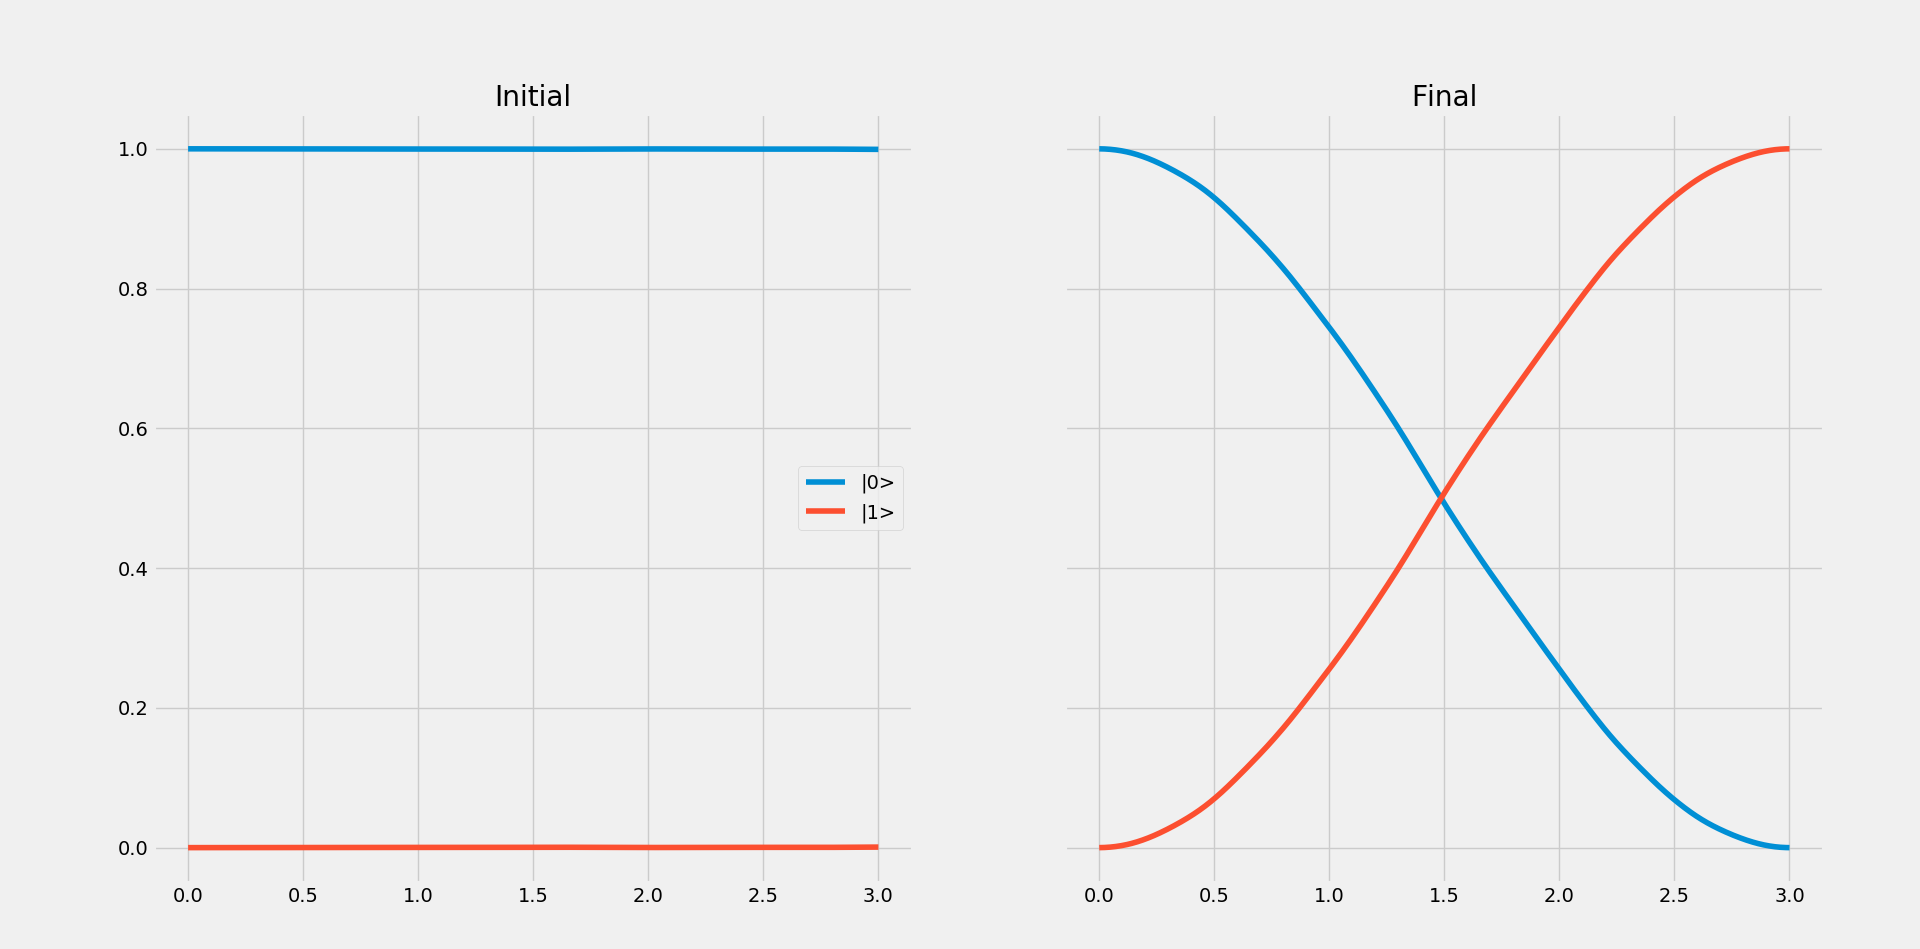
\includegraphics[width=1\columnwidth]{Results/qubit-band-amp-const/level-population.png}
%     \caption{Population of qubit levels over pulse duration. Before the optimization, the state of the qubit (population of ground and excited states) almost did not change at all. After the optimization, the qubit goes from state $\ket{0}$ to $\ket{1}$}
%     \label{fig:band-amp-const-level-population}
% \end{figure}
\begin{figure}[H]
    \begin{center}
        %% Creator: Matplotlib, PGF backend
%%
%% To include the figure in your LaTeX document, write
%%   \input{<filename>.pgf}
%%
%% Make sure the required packages are loaded in your preamble
%%   \usepackage{pgf}
%%
%% and, on pdftex
%%   \usepackage[utf8]{inputenc}\DeclareUnicodeCharacter{2212}{-}
%%
%% or, on luatex and xetex
%%   \usepackage{unicode-math}
%%
%% Figures using additional raster images can only be included by \input if
%% they are in the same directory as the main LaTeX file. For loading figures
%% from other directories you can use the `import` package
%%   \usepackage{import}
%%
%% and then include the figures with
%%   \import{<path to file>}{<filename>.pgf}
%%
%% Matplotlib used the following preamble
%%
\begingroup%
\makeatletter%
\begin{pgfpicture}%
\pgfpathrectangle{\pgfpointorigin}{\pgfqpoint{4.650000in}{2.300000in}}%
\pgfusepath{use as bounding box, clip}%
\begin{pgfscope}%
\pgfsetbuttcap%
\pgfsetmiterjoin%
\definecolor{currentfill}{rgb}{1.000000,1.000000,1.000000}%
\pgfsetfillcolor{currentfill}%
\pgfsetlinewidth{0.000000pt}%
\definecolor{currentstroke}{rgb}{1.000000,1.000000,1.000000}%
\pgfsetstrokecolor{currentstroke}%
\pgfsetdash{}{0pt}%
\pgfpathmoveto{\pgfqpoint{0.000000in}{0.000000in}}%
\pgfpathlineto{\pgfqpoint{4.650000in}{0.000000in}}%
\pgfpathlineto{\pgfqpoint{4.650000in}{2.300000in}}%
\pgfpathlineto{\pgfqpoint{0.000000in}{2.300000in}}%
\pgfpathclose%
\pgfusepath{fill}%
\end{pgfscope}%
\begin{pgfscope}%
\pgfsetbuttcap%
\pgfsetmiterjoin%
\definecolor{currentfill}{rgb}{1.000000,1.000000,1.000000}%
\pgfsetfillcolor{currentfill}%
\pgfsetlinewidth{0.000000pt}%
\definecolor{currentstroke}{rgb}{0.000000,0.000000,0.000000}%
\pgfsetstrokecolor{currentstroke}%
\pgfsetstrokeopacity{0.000000}%
\pgfsetdash{}{0pt}%
\pgfpathmoveto{\pgfqpoint{0.646914in}{0.370679in}}%
\pgfpathlineto{\pgfqpoint{2.474152in}{0.370679in}}%
\pgfpathlineto{\pgfqpoint{2.474152in}{1.927778in}}%
\pgfpathlineto{\pgfqpoint{0.646914in}{1.927778in}}%
\pgfpathclose%
\pgfusepath{fill}%
\end{pgfscope}%
\begin{pgfscope}%
\pgfpathrectangle{\pgfqpoint{0.646914in}{0.370679in}}{\pgfqpoint{1.827237in}{1.557099in}}%
\pgfusepath{clip}%
\pgfsetrectcap%
\pgfsetroundjoin%
\pgfsetlinewidth{0.803000pt}%
\definecolor{currentstroke}{rgb}{0.501961,0.501961,0.501961}%
\pgfsetstrokecolor{currentstroke}%
\pgfsetstrokeopacity{0.200000}%
\pgfsetdash{}{0pt}%
\pgfpathmoveto{\pgfqpoint{0.729970in}{0.370679in}}%
\pgfpathlineto{\pgfqpoint{0.729970in}{1.927778in}}%
\pgfusepath{stroke}%
\end{pgfscope}%
\begin{pgfscope}%
\pgfsetbuttcap%
\pgfsetroundjoin%
\definecolor{currentfill}{rgb}{0.333333,0.333333,0.333333}%
\pgfsetfillcolor{currentfill}%
\pgfsetlinewidth{0.803000pt}%
\definecolor{currentstroke}{rgb}{0.333333,0.333333,0.333333}%
\pgfsetstrokecolor{currentstroke}%
\pgfsetdash{}{0pt}%
\pgfsys@defobject{currentmarker}{\pgfqpoint{0.000000in}{-0.048611in}}{\pgfqpoint{0.000000in}{0.000000in}}{%
\pgfpathmoveto{\pgfqpoint{0.000000in}{0.000000in}}%
\pgfpathlineto{\pgfqpoint{0.000000in}{-0.048611in}}%
\pgfusepath{stroke,fill}%
}%
\begin{pgfscope}%
\pgfsys@transformshift{0.729970in}{0.370679in}%
\pgfsys@useobject{currentmarker}{}%
\end{pgfscope}%
\end{pgfscope}%
\begin{pgfscope}%
\definecolor{textcolor}{rgb}{0.333333,0.333333,0.333333}%
\pgfsetstrokecolor{textcolor}%
\pgfsetfillcolor{textcolor}%
\pgftext[x=0.729970in,y=0.273457in,,top]{\color{textcolor}\rmfamily\fontsize{10.000000}{12.000000}\selectfont \(\displaystyle {0}\)}%
\end{pgfscope}%
\begin{pgfscope}%
\pgfpathrectangle{\pgfqpoint{0.646914in}{0.370679in}}{\pgfqpoint{1.827237in}{1.557099in}}%
\pgfusepath{clip}%
\pgfsetrectcap%
\pgfsetroundjoin%
\pgfsetlinewidth{0.803000pt}%
\definecolor{currentstroke}{rgb}{0.501961,0.501961,0.501961}%
\pgfsetstrokecolor{currentstroke}%
\pgfsetstrokeopacity{0.200000}%
\pgfsetdash{}{0pt}%
\pgfpathmoveto{\pgfqpoint{1.394420in}{0.370679in}}%
\pgfpathlineto{\pgfqpoint{1.394420in}{1.927778in}}%
\pgfusepath{stroke}%
\end{pgfscope}%
\begin{pgfscope}%
\pgfsetbuttcap%
\pgfsetroundjoin%
\definecolor{currentfill}{rgb}{0.333333,0.333333,0.333333}%
\pgfsetfillcolor{currentfill}%
\pgfsetlinewidth{0.803000pt}%
\definecolor{currentstroke}{rgb}{0.333333,0.333333,0.333333}%
\pgfsetstrokecolor{currentstroke}%
\pgfsetdash{}{0pt}%
\pgfsys@defobject{currentmarker}{\pgfqpoint{0.000000in}{-0.048611in}}{\pgfqpoint{0.000000in}{0.000000in}}{%
\pgfpathmoveto{\pgfqpoint{0.000000in}{0.000000in}}%
\pgfpathlineto{\pgfqpoint{0.000000in}{-0.048611in}}%
\pgfusepath{stroke,fill}%
}%
\begin{pgfscope}%
\pgfsys@transformshift{1.394420in}{0.370679in}%
\pgfsys@useobject{currentmarker}{}%
\end{pgfscope}%
\end{pgfscope}%
\begin{pgfscope}%
\definecolor{textcolor}{rgb}{0.333333,0.333333,0.333333}%
\pgfsetstrokecolor{textcolor}%
\pgfsetfillcolor{textcolor}%
\pgftext[x=1.394420in,y=0.273457in,,top]{\color{textcolor}\rmfamily\fontsize{10.000000}{12.000000}\selectfont \(\displaystyle {10}\)}%
\end{pgfscope}%
\begin{pgfscope}%
\pgfpathrectangle{\pgfqpoint{0.646914in}{0.370679in}}{\pgfqpoint{1.827237in}{1.557099in}}%
\pgfusepath{clip}%
\pgfsetrectcap%
\pgfsetroundjoin%
\pgfsetlinewidth{0.803000pt}%
\definecolor{currentstroke}{rgb}{0.501961,0.501961,0.501961}%
\pgfsetstrokecolor{currentstroke}%
\pgfsetstrokeopacity{0.200000}%
\pgfsetdash{}{0pt}%
\pgfpathmoveto{\pgfqpoint{2.058870in}{0.370679in}}%
\pgfpathlineto{\pgfqpoint{2.058870in}{1.927778in}}%
\pgfusepath{stroke}%
\end{pgfscope}%
\begin{pgfscope}%
\pgfsetbuttcap%
\pgfsetroundjoin%
\definecolor{currentfill}{rgb}{0.333333,0.333333,0.333333}%
\pgfsetfillcolor{currentfill}%
\pgfsetlinewidth{0.803000pt}%
\definecolor{currentstroke}{rgb}{0.333333,0.333333,0.333333}%
\pgfsetstrokecolor{currentstroke}%
\pgfsetdash{}{0pt}%
\pgfsys@defobject{currentmarker}{\pgfqpoint{0.000000in}{-0.048611in}}{\pgfqpoint{0.000000in}{0.000000in}}{%
\pgfpathmoveto{\pgfqpoint{0.000000in}{0.000000in}}%
\pgfpathlineto{\pgfqpoint{0.000000in}{-0.048611in}}%
\pgfusepath{stroke,fill}%
}%
\begin{pgfscope}%
\pgfsys@transformshift{2.058870in}{0.370679in}%
\pgfsys@useobject{currentmarker}{}%
\end{pgfscope}%
\end{pgfscope}%
\begin{pgfscope}%
\definecolor{textcolor}{rgb}{0.333333,0.333333,0.333333}%
\pgfsetstrokecolor{textcolor}%
\pgfsetfillcolor{textcolor}%
\pgftext[x=2.058870in,y=0.273457in,,top]{\color{textcolor}\rmfamily\fontsize{10.000000}{12.000000}\selectfont \(\displaystyle {20}\)}%
\end{pgfscope}%
\begin{pgfscope}%
\pgfpathrectangle{\pgfqpoint{0.646914in}{0.370679in}}{\pgfqpoint{1.827237in}{1.557099in}}%
\pgfusepath{clip}%
\pgfsetrectcap%
\pgfsetroundjoin%
\pgfsetlinewidth{0.803000pt}%
\definecolor{currentstroke}{rgb}{0.501961,0.501961,0.501961}%
\pgfsetstrokecolor{currentstroke}%
\pgfsetstrokeopacity{0.200000}%
\pgfsetdash{}{0pt}%
\pgfpathmoveto{\pgfqpoint{0.646914in}{0.441456in}}%
\pgfpathlineto{\pgfqpoint{2.474152in}{0.441456in}}%
\pgfusepath{stroke}%
\end{pgfscope}%
\begin{pgfscope}%
\pgfsetbuttcap%
\pgfsetroundjoin%
\definecolor{currentfill}{rgb}{0.333333,0.333333,0.333333}%
\pgfsetfillcolor{currentfill}%
\pgfsetlinewidth{0.803000pt}%
\definecolor{currentstroke}{rgb}{0.333333,0.333333,0.333333}%
\pgfsetstrokecolor{currentstroke}%
\pgfsetdash{}{0pt}%
\pgfsys@defobject{currentmarker}{\pgfqpoint{-0.048611in}{0.000000in}}{\pgfqpoint{0.000000in}{0.000000in}}{%
\pgfpathmoveto{\pgfqpoint{0.000000in}{0.000000in}}%
\pgfpathlineto{\pgfqpoint{-0.048611in}{0.000000in}}%
\pgfusepath{stroke,fill}%
}%
\begin{pgfscope}%
\pgfsys@transformshift{0.646914in}{0.441456in}%
\pgfsys@useobject{currentmarker}{}%
\end{pgfscope}%
\end{pgfscope}%
\begin{pgfscope}%
\definecolor{textcolor}{rgb}{0.333333,0.333333,0.333333}%
\pgfsetstrokecolor{textcolor}%
\pgfsetfillcolor{textcolor}%
\pgftext[x=0.302778in, y=0.393231in, left, base]{\color{textcolor}\rmfamily\fontsize{10.000000}{12.000000}\selectfont \(\displaystyle {0.00}\)}%
\end{pgfscope}%
\begin{pgfscope}%
\pgfpathrectangle{\pgfqpoint{0.646914in}{0.370679in}}{\pgfqpoint{1.827237in}{1.557099in}}%
\pgfusepath{clip}%
\pgfsetrectcap%
\pgfsetroundjoin%
\pgfsetlinewidth{0.803000pt}%
\definecolor{currentstroke}{rgb}{0.501961,0.501961,0.501961}%
\pgfsetstrokecolor{currentstroke}%
\pgfsetstrokeopacity{0.200000}%
\pgfsetdash{}{0pt}%
\pgfpathmoveto{\pgfqpoint{0.646914in}{0.795342in}}%
\pgfpathlineto{\pgfqpoint{2.474152in}{0.795342in}}%
\pgfusepath{stroke}%
\end{pgfscope}%
\begin{pgfscope}%
\pgfsetbuttcap%
\pgfsetroundjoin%
\definecolor{currentfill}{rgb}{0.333333,0.333333,0.333333}%
\pgfsetfillcolor{currentfill}%
\pgfsetlinewidth{0.803000pt}%
\definecolor{currentstroke}{rgb}{0.333333,0.333333,0.333333}%
\pgfsetstrokecolor{currentstroke}%
\pgfsetdash{}{0pt}%
\pgfsys@defobject{currentmarker}{\pgfqpoint{-0.048611in}{0.000000in}}{\pgfqpoint{0.000000in}{0.000000in}}{%
\pgfpathmoveto{\pgfqpoint{0.000000in}{0.000000in}}%
\pgfpathlineto{\pgfqpoint{-0.048611in}{0.000000in}}%
\pgfusepath{stroke,fill}%
}%
\begin{pgfscope}%
\pgfsys@transformshift{0.646914in}{0.795342in}%
\pgfsys@useobject{currentmarker}{}%
\end{pgfscope}%
\end{pgfscope}%
\begin{pgfscope}%
\definecolor{textcolor}{rgb}{0.333333,0.333333,0.333333}%
\pgfsetstrokecolor{textcolor}%
\pgfsetfillcolor{textcolor}%
\pgftext[x=0.302778in, y=0.747117in, left, base]{\color{textcolor}\rmfamily\fontsize{10.000000}{12.000000}\selectfont \(\displaystyle {0.25}\)}%
\end{pgfscope}%
\begin{pgfscope}%
\pgfpathrectangle{\pgfqpoint{0.646914in}{0.370679in}}{\pgfqpoint{1.827237in}{1.557099in}}%
\pgfusepath{clip}%
\pgfsetrectcap%
\pgfsetroundjoin%
\pgfsetlinewidth{0.803000pt}%
\definecolor{currentstroke}{rgb}{0.501961,0.501961,0.501961}%
\pgfsetstrokecolor{currentstroke}%
\pgfsetstrokeopacity{0.200000}%
\pgfsetdash{}{0pt}%
\pgfpathmoveto{\pgfqpoint{0.646914in}{1.149228in}}%
\pgfpathlineto{\pgfqpoint{2.474152in}{1.149228in}}%
\pgfusepath{stroke}%
\end{pgfscope}%
\begin{pgfscope}%
\pgfsetbuttcap%
\pgfsetroundjoin%
\definecolor{currentfill}{rgb}{0.333333,0.333333,0.333333}%
\pgfsetfillcolor{currentfill}%
\pgfsetlinewidth{0.803000pt}%
\definecolor{currentstroke}{rgb}{0.333333,0.333333,0.333333}%
\pgfsetstrokecolor{currentstroke}%
\pgfsetdash{}{0pt}%
\pgfsys@defobject{currentmarker}{\pgfqpoint{-0.048611in}{0.000000in}}{\pgfqpoint{0.000000in}{0.000000in}}{%
\pgfpathmoveto{\pgfqpoint{0.000000in}{0.000000in}}%
\pgfpathlineto{\pgfqpoint{-0.048611in}{0.000000in}}%
\pgfusepath{stroke,fill}%
}%
\begin{pgfscope}%
\pgfsys@transformshift{0.646914in}{1.149228in}%
\pgfsys@useobject{currentmarker}{}%
\end{pgfscope}%
\end{pgfscope}%
\begin{pgfscope}%
\definecolor{textcolor}{rgb}{0.333333,0.333333,0.333333}%
\pgfsetstrokecolor{textcolor}%
\pgfsetfillcolor{textcolor}%
\pgftext[x=0.302778in, y=1.101003in, left, base]{\color{textcolor}\rmfamily\fontsize{10.000000}{12.000000}\selectfont \(\displaystyle {0.50}\)}%
\end{pgfscope}%
\begin{pgfscope}%
\pgfpathrectangle{\pgfqpoint{0.646914in}{0.370679in}}{\pgfqpoint{1.827237in}{1.557099in}}%
\pgfusepath{clip}%
\pgfsetrectcap%
\pgfsetroundjoin%
\pgfsetlinewidth{0.803000pt}%
\definecolor{currentstroke}{rgb}{0.501961,0.501961,0.501961}%
\pgfsetstrokecolor{currentstroke}%
\pgfsetstrokeopacity{0.200000}%
\pgfsetdash{}{0pt}%
\pgfpathmoveto{\pgfqpoint{0.646914in}{1.503115in}}%
\pgfpathlineto{\pgfqpoint{2.474152in}{1.503115in}}%
\pgfusepath{stroke}%
\end{pgfscope}%
\begin{pgfscope}%
\pgfsetbuttcap%
\pgfsetroundjoin%
\definecolor{currentfill}{rgb}{0.333333,0.333333,0.333333}%
\pgfsetfillcolor{currentfill}%
\pgfsetlinewidth{0.803000pt}%
\definecolor{currentstroke}{rgb}{0.333333,0.333333,0.333333}%
\pgfsetstrokecolor{currentstroke}%
\pgfsetdash{}{0pt}%
\pgfsys@defobject{currentmarker}{\pgfqpoint{-0.048611in}{0.000000in}}{\pgfqpoint{0.000000in}{0.000000in}}{%
\pgfpathmoveto{\pgfqpoint{0.000000in}{0.000000in}}%
\pgfpathlineto{\pgfqpoint{-0.048611in}{0.000000in}}%
\pgfusepath{stroke,fill}%
}%
\begin{pgfscope}%
\pgfsys@transformshift{0.646914in}{1.503115in}%
\pgfsys@useobject{currentmarker}{}%
\end{pgfscope}%
\end{pgfscope}%
\begin{pgfscope}%
\definecolor{textcolor}{rgb}{0.333333,0.333333,0.333333}%
\pgfsetstrokecolor{textcolor}%
\pgfsetfillcolor{textcolor}%
\pgftext[x=0.302778in, y=1.454889in, left, base]{\color{textcolor}\rmfamily\fontsize{10.000000}{12.000000}\selectfont \(\displaystyle {0.75}\)}%
\end{pgfscope}%
\begin{pgfscope}%
\pgfpathrectangle{\pgfqpoint{0.646914in}{0.370679in}}{\pgfqpoint{1.827237in}{1.557099in}}%
\pgfusepath{clip}%
\pgfsetrectcap%
\pgfsetroundjoin%
\pgfsetlinewidth{0.803000pt}%
\definecolor{currentstroke}{rgb}{0.501961,0.501961,0.501961}%
\pgfsetstrokecolor{currentstroke}%
\pgfsetstrokeopacity{0.200000}%
\pgfsetdash{}{0pt}%
\pgfpathmoveto{\pgfqpoint{0.646914in}{1.857001in}}%
\pgfpathlineto{\pgfqpoint{2.474152in}{1.857001in}}%
\pgfusepath{stroke}%
\end{pgfscope}%
\begin{pgfscope}%
\pgfsetbuttcap%
\pgfsetroundjoin%
\definecolor{currentfill}{rgb}{0.333333,0.333333,0.333333}%
\pgfsetfillcolor{currentfill}%
\pgfsetlinewidth{0.803000pt}%
\definecolor{currentstroke}{rgb}{0.333333,0.333333,0.333333}%
\pgfsetstrokecolor{currentstroke}%
\pgfsetdash{}{0pt}%
\pgfsys@defobject{currentmarker}{\pgfqpoint{-0.048611in}{0.000000in}}{\pgfqpoint{0.000000in}{0.000000in}}{%
\pgfpathmoveto{\pgfqpoint{0.000000in}{0.000000in}}%
\pgfpathlineto{\pgfqpoint{-0.048611in}{0.000000in}}%
\pgfusepath{stroke,fill}%
}%
\begin{pgfscope}%
\pgfsys@transformshift{0.646914in}{1.857001in}%
\pgfsys@useobject{currentmarker}{}%
\end{pgfscope}%
\end{pgfscope}%
\begin{pgfscope}%
\definecolor{textcolor}{rgb}{0.333333,0.333333,0.333333}%
\pgfsetstrokecolor{textcolor}%
\pgfsetfillcolor{textcolor}%
\pgftext[x=0.302778in, y=1.808776in, left, base]{\color{textcolor}\rmfamily\fontsize{10.000000}{12.000000}\selectfont \(\displaystyle {1.00}\)}%
\end{pgfscope}%
\begin{pgfscope}%
\definecolor{textcolor}{rgb}{0.333333,0.333333,0.333333}%
\pgfsetstrokecolor{textcolor}%
\pgfsetfillcolor{textcolor}%
\pgftext[x=0.247222in,y=1.149228in,,bottom,rotate=90.000000]{\color{textcolor}\rmfamily\fontsize{12.000000}{14.400000}\selectfont Amplitude (MHz)}%
\end{pgfscope}%
\begin{pgfscope}%
\pgfpathrectangle{\pgfqpoint{0.646914in}{0.370679in}}{\pgfqpoint{1.827237in}{1.557099in}}%
\pgfusepath{clip}%
\pgfsetrectcap%
\pgfsetroundjoin%
\pgfsetlinewidth{1.505625pt}%
\definecolor{currentstroke}{rgb}{0.886275,0.290196,0.200000}%
\pgfsetstrokecolor{currentstroke}%
\pgfsetdash{}{0pt}%
\pgfpathmoveto{\pgfqpoint{0.729970in}{1.857001in}}%
\pgfpathlineto{\pgfqpoint{2.391095in}{1.856987in}}%
\pgfpathlineto{\pgfqpoint{2.391095in}{1.856987in}}%
\pgfusepath{stroke}%
\end{pgfscope}%
\begin{pgfscope}%
\pgfpathrectangle{\pgfqpoint{0.646914in}{0.370679in}}{\pgfqpoint{1.827237in}{1.557099in}}%
\pgfusepath{clip}%
\pgfsetrectcap%
\pgfsetroundjoin%
\pgfsetlinewidth{1.505625pt}%
\definecolor{currentstroke}{rgb}{0.203922,0.541176,0.741176}%
\pgfsetstrokecolor{currentstroke}%
\pgfsetdash{}{0pt}%
\pgfpathmoveto{\pgfqpoint{0.729970in}{0.441456in}}%
\pgfpathlineto{\pgfqpoint{2.391095in}{0.441469in}}%
\pgfpathlineto{\pgfqpoint{2.391095in}{0.441469in}}%
\pgfusepath{stroke}%
\end{pgfscope}%
\begin{pgfscope}%
\pgfsetrectcap%
\pgfsetmiterjoin%
\pgfsetlinewidth{1.003750pt}%
\definecolor{currentstroke}{rgb}{1.000000,1.000000,1.000000}%
\pgfsetstrokecolor{currentstroke}%
\pgfsetdash{}{0pt}%
\pgfpathmoveto{\pgfqpoint{0.646914in}{0.370679in}}%
\pgfpathlineto{\pgfqpoint{0.646914in}{1.927778in}}%
\pgfusepath{stroke}%
\end{pgfscope}%
\begin{pgfscope}%
\pgfsetrectcap%
\pgfsetmiterjoin%
\pgfsetlinewidth{1.003750pt}%
\definecolor{currentstroke}{rgb}{1.000000,1.000000,1.000000}%
\pgfsetstrokecolor{currentstroke}%
\pgfsetdash{}{0pt}%
\pgfpathmoveto{\pgfqpoint{2.474152in}{0.370679in}}%
\pgfpathlineto{\pgfqpoint{2.474152in}{1.927778in}}%
\pgfusepath{stroke}%
\end{pgfscope}%
\begin{pgfscope}%
\pgfsetrectcap%
\pgfsetmiterjoin%
\pgfsetlinewidth{1.003750pt}%
\definecolor{currentstroke}{rgb}{1.000000,1.000000,1.000000}%
\pgfsetstrokecolor{currentstroke}%
\pgfsetdash{}{0pt}%
\pgfpathmoveto{\pgfqpoint{0.646914in}{0.370679in}}%
\pgfpathlineto{\pgfqpoint{2.474152in}{0.370679in}}%
\pgfusepath{stroke}%
\end{pgfscope}%
\begin{pgfscope}%
\pgfsetrectcap%
\pgfsetmiterjoin%
\pgfsetlinewidth{1.003750pt}%
\definecolor{currentstroke}{rgb}{1.000000,1.000000,1.000000}%
\pgfsetstrokecolor{currentstroke}%
\pgfsetdash{}{0pt}%
\pgfpathmoveto{\pgfqpoint{0.646914in}{1.927778in}}%
\pgfpathlineto{\pgfqpoint{2.474152in}{1.927778in}}%
\pgfusepath{stroke}%
\end{pgfscope}%
\begin{pgfscope}%
\definecolor{textcolor}{rgb}{0.000000,0.000000,0.000000}%
\pgfsetstrokecolor{textcolor}%
\pgfsetfillcolor{textcolor}%
\pgftext[x=1.560533in,y=2.011111in,,base]{\color{textcolor}\rmfamily\fontsize{14.400000}{17.280000}\selectfont Initial pulse}%
\end{pgfscope}%
\begin{pgfscope}%
\pgfsetbuttcap%
\pgfsetmiterjoin%
\definecolor{currentfill}{rgb}{1.000000,1.000000,1.000000}%
\pgfsetfillcolor{currentfill}%
\pgfsetfillopacity{0.800000}%
\pgfsetlinewidth{0.501875pt}%
\definecolor{currentstroke}{rgb}{0.800000,0.800000,0.800000}%
\pgfsetstrokecolor{currentstroke}%
\pgfsetstrokeopacity{0.800000}%
\pgfsetdash{}{0pt}%
\pgfpathmoveto{\pgfqpoint{1.552179in}{0.920062in}}%
\pgfpathlineto{\pgfqpoint{2.376929in}{0.920062in}}%
\pgfpathquadraticcurveto{\pgfqpoint{2.404707in}{0.920062in}}{\pgfqpoint{2.404707in}{0.947840in}}%
\pgfpathlineto{\pgfqpoint{2.404707in}{1.350617in}}%
\pgfpathquadraticcurveto{\pgfqpoint{2.404707in}{1.378395in}}{\pgfqpoint{2.376929in}{1.378395in}}%
\pgfpathlineto{\pgfqpoint{1.552179in}{1.378395in}}%
\pgfpathquadraticcurveto{\pgfqpoint{1.524402in}{1.378395in}}{\pgfqpoint{1.524402in}{1.350617in}}%
\pgfpathlineto{\pgfqpoint{1.524402in}{0.947840in}}%
\pgfpathquadraticcurveto{\pgfqpoint{1.524402in}{0.920062in}}{\pgfqpoint{1.552179in}{0.920062in}}%
\pgfpathclose%
\pgfusepath{stroke,fill}%
\end{pgfscope}%
\begin{pgfscope}%
\pgfsetrectcap%
\pgfsetroundjoin%
\pgfsetlinewidth{1.505625pt}%
\definecolor{currentstroke}{rgb}{0.886275,0.290196,0.200000}%
\pgfsetstrokecolor{currentstroke}%
\pgfsetdash{}{0pt}%
\pgfpathmoveto{\pgfqpoint{1.579957in}{1.267284in}}%
\pgfpathlineto{\pgfqpoint{1.857735in}{1.267284in}}%
\pgfusepath{stroke}%
\end{pgfscope}%
\begin{pgfscope}%
\definecolor{textcolor}{rgb}{0.000000,0.000000,0.000000}%
\pgfsetstrokecolor{textcolor}%
\pgfsetfillcolor{textcolor}%
\pgftext[x=1.968846in,y=1.218673in,left,base]{\color{textcolor}\rmfamily\fontsize{10.000000}{12.000000}\selectfont \(\displaystyle P(|g\rangle)\)}%
\end{pgfscope}%
\begin{pgfscope}%
\pgfsetrectcap%
\pgfsetroundjoin%
\pgfsetlinewidth{1.505625pt}%
\definecolor{currentstroke}{rgb}{0.203922,0.541176,0.741176}%
\pgfsetstrokecolor{currentstroke}%
\pgfsetdash{}{0pt}%
\pgfpathmoveto{\pgfqpoint{1.579957in}{1.058951in}}%
\pgfpathlineto{\pgfqpoint{1.857735in}{1.058951in}}%
\pgfusepath{stroke}%
\end{pgfscope}%
\begin{pgfscope}%
\definecolor{textcolor}{rgb}{0.000000,0.000000,0.000000}%
\pgfsetstrokecolor{textcolor}%
\pgfsetfillcolor{textcolor}%
\pgftext[x=1.968846in,y=1.010340in,left,base]{\color{textcolor}\rmfamily\fontsize{10.000000}{12.000000}\selectfont \(\displaystyle P(|e\rangle)\)}%
\end{pgfscope}%
\begin{pgfscope}%
\pgfsetbuttcap%
\pgfsetmiterjoin%
\definecolor{currentfill}{rgb}{1.000000,1.000000,1.000000}%
\pgfsetfillcolor{currentfill}%
\pgfsetlinewidth{0.000000pt}%
\definecolor{currentstroke}{rgb}{0.000000,0.000000,0.000000}%
\pgfsetstrokecolor{currentstroke}%
\pgfsetstrokeopacity{0.000000}%
\pgfsetdash{}{0pt}%
\pgfpathmoveto{\pgfqpoint{2.672763in}{0.370679in}}%
\pgfpathlineto{\pgfqpoint{4.500000in}{0.370679in}}%
\pgfpathlineto{\pgfqpoint{4.500000in}{1.927778in}}%
\pgfpathlineto{\pgfqpoint{2.672763in}{1.927778in}}%
\pgfpathclose%
\pgfusepath{fill}%
\end{pgfscope}%
\begin{pgfscope}%
\pgfpathrectangle{\pgfqpoint{2.672763in}{0.370679in}}{\pgfqpoint{1.827237in}{1.557099in}}%
\pgfusepath{clip}%
\pgfsetrectcap%
\pgfsetroundjoin%
\pgfsetlinewidth{0.803000pt}%
\definecolor{currentstroke}{rgb}{0.501961,0.501961,0.501961}%
\pgfsetstrokecolor{currentstroke}%
\pgfsetstrokeopacity{0.200000}%
\pgfsetdash{}{0pt}%
\pgfpathmoveto{\pgfqpoint{2.755819in}{0.370679in}}%
\pgfpathlineto{\pgfqpoint{2.755819in}{1.927778in}}%
\pgfusepath{stroke}%
\end{pgfscope}%
\begin{pgfscope}%
\pgfsetbuttcap%
\pgfsetroundjoin%
\definecolor{currentfill}{rgb}{0.333333,0.333333,0.333333}%
\pgfsetfillcolor{currentfill}%
\pgfsetlinewidth{0.803000pt}%
\definecolor{currentstroke}{rgb}{0.333333,0.333333,0.333333}%
\pgfsetstrokecolor{currentstroke}%
\pgfsetdash{}{0pt}%
\pgfsys@defobject{currentmarker}{\pgfqpoint{0.000000in}{-0.048611in}}{\pgfqpoint{0.000000in}{0.000000in}}{%
\pgfpathmoveto{\pgfqpoint{0.000000in}{0.000000in}}%
\pgfpathlineto{\pgfqpoint{0.000000in}{-0.048611in}}%
\pgfusepath{stroke,fill}%
}%
\begin{pgfscope}%
\pgfsys@transformshift{2.755819in}{0.370679in}%
\pgfsys@useobject{currentmarker}{}%
\end{pgfscope}%
\end{pgfscope}%
\begin{pgfscope}%
\definecolor{textcolor}{rgb}{0.333333,0.333333,0.333333}%
\pgfsetstrokecolor{textcolor}%
\pgfsetfillcolor{textcolor}%
\pgftext[x=2.755819in,y=0.273457in,,top]{\color{textcolor}\rmfamily\fontsize{10.000000}{12.000000}\selectfont \(\displaystyle {0}\)}%
\end{pgfscope}%
\begin{pgfscope}%
\pgfpathrectangle{\pgfqpoint{2.672763in}{0.370679in}}{\pgfqpoint{1.827237in}{1.557099in}}%
\pgfusepath{clip}%
\pgfsetrectcap%
\pgfsetroundjoin%
\pgfsetlinewidth{0.803000pt}%
\definecolor{currentstroke}{rgb}{0.501961,0.501961,0.501961}%
\pgfsetstrokecolor{currentstroke}%
\pgfsetstrokeopacity{0.200000}%
\pgfsetdash{}{0pt}%
\pgfpathmoveto{\pgfqpoint{3.420269in}{0.370679in}}%
\pgfpathlineto{\pgfqpoint{3.420269in}{1.927778in}}%
\pgfusepath{stroke}%
\end{pgfscope}%
\begin{pgfscope}%
\pgfsetbuttcap%
\pgfsetroundjoin%
\definecolor{currentfill}{rgb}{0.333333,0.333333,0.333333}%
\pgfsetfillcolor{currentfill}%
\pgfsetlinewidth{0.803000pt}%
\definecolor{currentstroke}{rgb}{0.333333,0.333333,0.333333}%
\pgfsetstrokecolor{currentstroke}%
\pgfsetdash{}{0pt}%
\pgfsys@defobject{currentmarker}{\pgfqpoint{0.000000in}{-0.048611in}}{\pgfqpoint{0.000000in}{0.000000in}}{%
\pgfpathmoveto{\pgfqpoint{0.000000in}{0.000000in}}%
\pgfpathlineto{\pgfqpoint{0.000000in}{-0.048611in}}%
\pgfusepath{stroke,fill}%
}%
\begin{pgfscope}%
\pgfsys@transformshift{3.420269in}{0.370679in}%
\pgfsys@useobject{currentmarker}{}%
\end{pgfscope}%
\end{pgfscope}%
\begin{pgfscope}%
\definecolor{textcolor}{rgb}{0.333333,0.333333,0.333333}%
\pgfsetstrokecolor{textcolor}%
\pgfsetfillcolor{textcolor}%
\pgftext[x=3.420269in,y=0.273457in,,top]{\color{textcolor}\rmfamily\fontsize{10.000000}{12.000000}\selectfont \(\displaystyle {10}\)}%
\end{pgfscope}%
\begin{pgfscope}%
\pgfpathrectangle{\pgfqpoint{2.672763in}{0.370679in}}{\pgfqpoint{1.827237in}{1.557099in}}%
\pgfusepath{clip}%
\pgfsetrectcap%
\pgfsetroundjoin%
\pgfsetlinewidth{0.803000pt}%
\definecolor{currentstroke}{rgb}{0.501961,0.501961,0.501961}%
\pgfsetstrokecolor{currentstroke}%
\pgfsetstrokeopacity{0.200000}%
\pgfsetdash{}{0pt}%
\pgfpathmoveto{\pgfqpoint{4.084719in}{0.370679in}}%
\pgfpathlineto{\pgfqpoint{4.084719in}{1.927778in}}%
\pgfusepath{stroke}%
\end{pgfscope}%
\begin{pgfscope}%
\pgfsetbuttcap%
\pgfsetroundjoin%
\definecolor{currentfill}{rgb}{0.333333,0.333333,0.333333}%
\pgfsetfillcolor{currentfill}%
\pgfsetlinewidth{0.803000pt}%
\definecolor{currentstroke}{rgb}{0.333333,0.333333,0.333333}%
\pgfsetstrokecolor{currentstroke}%
\pgfsetdash{}{0pt}%
\pgfsys@defobject{currentmarker}{\pgfqpoint{0.000000in}{-0.048611in}}{\pgfqpoint{0.000000in}{0.000000in}}{%
\pgfpathmoveto{\pgfqpoint{0.000000in}{0.000000in}}%
\pgfpathlineto{\pgfqpoint{0.000000in}{-0.048611in}}%
\pgfusepath{stroke,fill}%
}%
\begin{pgfscope}%
\pgfsys@transformshift{4.084719in}{0.370679in}%
\pgfsys@useobject{currentmarker}{}%
\end{pgfscope}%
\end{pgfscope}%
\begin{pgfscope}%
\definecolor{textcolor}{rgb}{0.333333,0.333333,0.333333}%
\pgfsetstrokecolor{textcolor}%
\pgfsetfillcolor{textcolor}%
\pgftext[x=4.084719in,y=0.273457in,,top]{\color{textcolor}\rmfamily\fontsize{10.000000}{12.000000}\selectfont \(\displaystyle {20}\)}%
\end{pgfscope}%
\begin{pgfscope}%
\pgfpathrectangle{\pgfqpoint{2.672763in}{0.370679in}}{\pgfqpoint{1.827237in}{1.557099in}}%
\pgfusepath{clip}%
\pgfsetrectcap%
\pgfsetroundjoin%
\pgfsetlinewidth{0.803000pt}%
\definecolor{currentstroke}{rgb}{0.501961,0.501961,0.501961}%
\pgfsetstrokecolor{currentstroke}%
\pgfsetstrokeopacity{0.200000}%
\pgfsetdash{}{0pt}%
\pgfpathmoveto{\pgfqpoint{2.672763in}{0.441456in}}%
\pgfpathlineto{\pgfqpoint{4.500000in}{0.441456in}}%
\pgfusepath{stroke}%
\end{pgfscope}%
\begin{pgfscope}%
\pgfsetbuttcap%
\pgfsetroundjoin%
\definecolor{currentfill}{rgb}{0.333333,0.333333,0.333333}%
\pgfsetfillcolor{currentfill}%
\pgfsetlinewidth{0.803000pt}%
\definecolor{currentstroke}{rgb}{0.333333,0.333333,0.333333}%
\pgfsetstrokecolor{currentstroke}%
\pgfsetdash{}{0pt}%
\pgfsys@defobject{currentmarker}{\pgfqpoint{-0.048611in}{0.000000in}}{\pgfqpoint{0.000000in}{0.000000in}}{%
\pgfpathmoveto{\pgfqpoint{0.000000in}{0.000000in}}%
\pgfpathlineto{\pgfqpoint{-0.048611in}{0.000000in}}%
\pgfusepath{stroke,fill}%
}%
\begin{pgfscope}%
\pgfsys@transformshift{2.672763in}{0.441456in}%
\pgfsys@useobject{currentmarker}{}%
\end{pgfscope}%
\end{pgfscope}%
\begin{pgfscope}%
\pgfpathrectangle{\pgfqpoint{2.672763in}{0.370679in}}{\pgfqpoint{1.827237in}{1.557099in}}%
\pgfusepath{clip}%
\pgfsetrectcap%
\pgfsetroundjoin%
\pgfsetlinewidth{0.803000pt}%
\definecolor{currentstroke}{rgb}{0.501961,0.501961,0.501961}%
\pgfsetstrokecolor{currentstroke}%
\pgfsetstrokeopacity{0.200000}%
\pgfsetdash{}{0pt}%
\pgfpathmoveto{\pgfqpoint{2.672763in}{0.795342in}}%
\pgfpathlineto{\pgfqpoint{4.500000in}{0.795342in}}%
\pgfusepath{stroke}%
\end{pgfscope}%
\begin{pgfscope}%
\pgfsetbuttcap%
\pgfsetroundjoin%
\definecolor{currentfill}{rgb}{0.333333,0.333333,0.333333}%
\pgfsetfillcolor{currentfill}%
\pgfsetlinewidth{0.803000pt}%
\definecolor{currentstroke}{rgb}{0.333333,0.333333,0.333333}%
\pgfsetstrokecolor{currentstroke}%
\pgfsetdash{}{0pt}%
\pgfsys@defobject{currentmarker}{\pgfqpoint{-0.048611in}{0.000000in}}{\pgfqpoint{0.000000in}{0.000000in}}{%
\pgfpathmoveto{\pgfqpoint{0.000000in}{0.000000in}}%
\pgfpathlineto{\pgfqpoint{-0.048611in}{0.000000in}}%
\pgfusepath{stroke,fill}%
}%
\begin{pgfscope}%
\pgfsys@transformshift{2.672763in}{0.795342in}%
\pgfsys@useobject{currentmarker}{}%
\end{pgfscope}%
\end{pgfscope}%
\begin{pgfscope}%
\pgfpathrectangle{\pgfqpoint{2.672763in}{0.370679in}}{\pgfqpoint{1.827237in}{1.557099in}}%
\pgfusepath{clip}%
\pgfsetrectcap%
\pgfsetroundjoin%
\pgfsetlinewidth{0.803000pt}%
\definecolor{currentstroke}{rgb}{0.501961,0.501961,0.501961}%
\pgfsetstrokecolor{currentstroke}%
\pgfsetstrokeopacity{0.200000}%
\pgfsetdash{}{0pt}%
\pgfpathmoveto{\pgfqpoint{2.672763in}{1.149228in}}%
\pgfpathlineto{\pgfqpoint{4.500000in}{1.149228in}}%
\pgfusepath{stroke}%
\end{pgfscope}%
\begin{pgfscope}%
\pgfsetbuttcap%
\pgfsetroundjoin%
\definecolor{currentfill}{rgb}{0.333333,0.333333,0.333333}%
\pgfsetfillcolor{currentfill}%
\pgfsetlinewidth{0.803000pt}%
\definecolor{currentstroke}{rgb}{0.333333,0.333333,0.333333}%
\pgfsetstrokecolor{currentstroke}%
\pgfsetdash{}{0pt}%
\pgfsys@defobject{currentmarker}{\pgfqpoint{-0.048611in}{0.000000in}}{\pgfqpoint{0.000000in}{0.000000in}}{%
\pgfpathmoveto{\pgfqpoint{0.000000in}{0.000000in}}%
\pgfpathlineto{\pgfqpoint{-0.048611in}{0.000000in}}%
\pgfusepath{stroke,fill}%
}%
\begin{pgfscope}%
\pgfsys@transformshift{2.672763in}{1.149228in}%
\pgfsys@useobject{currentmarker}{}%
\end{pgfscope}%
\end{pgfscope}%
\begin{pgfscope}%
\pgfpathrectangle{\pgfqpoint{2.672763in}{0.370679in}}{\pgfqpoint{1.827237in}{1.557099in}}%
\pgfusepath{clip}%
\pgfsetrectcap%
\pgfsetroundjoin%
\pgfsetlinewidth{0.803000pt}%
\definecolor{currentstroke}{rgb}{0.501961,0.501961,0.501961}%
\pgfsetstrokecolor{currentstroke}%
\pgfsetstrokeopacity{0.200000}%
\pgfsetdash{}{0pt}%
\pgfpathmoveto{\pgfqpoint{2.672763in}{1.503115in}}%
\pgfpathlineto{\pgfqpoint{4.500000in}{1.503115in}}%
\pgfusepath{stroke}%
\end{pgfscope}%
\begin{pgfscope}%
\pgfsetbuttcap%
\pgfsetroundjoin%
\definecolor{currentfill}{rgb}{0.333333,0.333333,0.333333}%
\pgfsetfillcolor{currentfill}%
\pgfsetlinewidth{0.803000pt}%
\definecolor{currentstroke}{rgb}{0.333333,0.333333,0.333333}%
\pgfsetstrokecolor{currentstroke}%
\pgfsetdash{}{0pt}%
\pgfsys@defobject{currentmarker}{\pgfqpoint{-0.048611in}{0.000000in}}{\pgfqpoint{0.000000in}{0.000000in}}{%
\pgfpathmoveto{\pgfqpoint{0.000000in}{0.000000in}}%
\pgfpathlineto{\pgfqpoint{-0.048611in}{0.000000in}}%
\pgfusepath{stroke,fill}%
}%
\begin{pgfscope}%
\pgfsys@transformshift{2.672763in}{1.503115in}%
\pgfsys@useobject{currentmarker}{}%
\end{pgfscope}%
\end{pgfscope}%
\begin{pgfscope}%
\pgfpathrectangle{\pgfqpoint{2.672763in}{0.370679in}}{\pgfqpoint{1.827237in}{1.557099in}}%
\pgfusepath{clip}%
\pgfsetrectcap%
\pgfsetroundjoin%
\pgfsetlinewidth{0.803000pt}%
\definecolor{currentstroke}{rgb}{0.501961,0.501961,0.501961}%
\pgfsetstrokecolor{currentstroke}%
\pgfsetstrokeopacity{0.200000}%
\pgfsetdash{}{0pt}%
\pgfpathmoveto{\pgfqpoint{2.672763in}{1.857001in}}%
\pgfpathlineto{\pgfqpoint{4.500000in}{1.857001in}}%
\pgfusepath{stroke}%
\end{pgfscope}%
\begin{pgfscope}%
\pgfsetbuttcap%
\pgfsetroundjoin%
\definecolor{currentfill}{rgb}{0.333333,0.333333,0.333333}%
\pgfsetfillcolor{currentfill}%
\pgfsetlinewidth{0.803000pt}%
\definecolor{currentstroke}{rgb}{0.333333,0.333333,0.333333}%
\pgfsetstrokecolor{currentstroke}%
\pgfsetdash{}{0pt}%
\pgfsys@defobject{currentmarker}{\pgfqpoint{-0.048611in}{0.000000in}}{\pgfqpoint{0.000000in}{0.000000in}}{%
\pgfpathmoveto{\pgfqpoint{0.000000in}{0.000000in}}%
\pgfpathlineto{\pgfqpoint{-0.048611in}{0.000000in}}%
\pgfusepath{stroke,fill}%
}%
\begin{pgfscope}%
\pgfsys@transformshift{2.672763in}{1.857001in}%
\pgfsys@useobject{currentmarker}{}%
\end{pgfscope}%
\end{pgfscope}%
\begin{pgfscope}%
\pgfpathrectangle{\pgfqpoint{2.672763in}{0.370679in}}{\pgfqpoint{1.827237in}{1.557099in}}%
\pgfusepath{clip}%
\pgfsetrectcap%
\pgfsetroundjoin%
\pgfsetlinewidth{1.505625pt}%
\definecolor{currentstroke}{rgb}{0.886275,0.290196,0.200000}%
\pgfsetstrokecolor{currentstroke}%
\pgfsetdash{}{0pt}%
\pgfpathmoveto{\pgfqpoint{2.755819in}{1.856915in}}%
\pgfpathlineto{\pgfqpoint{2.789208in}{1.854853in}}%
\pgfpathlineto{\pgfqpoint{2.822598in}{1.849998in}}%
\pgfpathlineto{\pgfqpoint{2.855987in}{1.842205in}}%
\pgfpathlineto{\pgfqpoint{2.889377in}{1.831577in}}%
\pgfpathlineto{\pgfqpoint{2.922766in}{1.818382in}}%
\pgfpathlineto{\pgfqpoint{2.964503in}{1.797995in}}%
\pgfpathlineto{\pgfqpoint{3.006240in}{1.773568in}}%
\pgfpathlineto{\pgfqpoint{3.047977in}{1.745323in}}%
\pgfpathlineto{\pgfqpoint{3.098061in}{1.707292in}}%
\pgfpathlineto{\pgfqpoint{3.148145in}{1.663981in}}%
\pgfpathlineto{\pgfqpoint{3.189882in}{1.624561in}}%
\pgfpathlineto{\pgfqpoint{3.239966in}{1.573058in}}%
\pgfpathlineto{\pgfqpoint{3.298397in}{1.508591in}}%
\pgfpathlineto{\pgfqpoint{3.348482in}{1.449914in}}%
\pgfpathlineto{\pgfqpoint{3.415260in}{1.365946in}}%
\pgfpathlineto{\pgfqpoint{3.565513in}{1.170061in}}%
\pgfpathlineto{\pgfqpoint{3.732460in}{0.950177in}}%
\pgfpathlineto{\pgfqpoint{3.815934in}{0.847804in}}%
\pgfpathlineto{\pgfqpoint{3.891060in}{0.761994in}}%
\pgfpathlineto{\pgfqpoint{3.949492in}{0.699613in}}%
\pgfpathlineto{\pgfqpoint{3.999576in}{0.649561in}}%
\pgfpathlineto{\pgfqpoint{4.049660in}{0.604309in}}%
\pgfpathlineto{\pgfqpoint{4.091397in}{0.570493in}}%
\pgfpathlineto{\pgfqpoint{4.141481in}{0.534391in}}%
\pgfpathlineto{\pgfqpoint{4.183218in}{0.508237in}}%
\pgfpathlineto{\pgfqpoint{4.224954in}{0.486459in}}%
\pgfpathlineto{\pgfqpoint{4.258344in}{0.472265in}}%
\pgfpathlineto{\pgfqpoint{4.300081in}{0.458408in}}%
\pgfpathlineto{\pgfqpoint{4.333470in}{0.450132in}}%
\pgfpathlineto{\pgfqpoint{4.366860in}{0.444555in}}%
\pgfpathlineto{\pgfqpoint{4.400249in}{0.441789in}}%
\pgfpathlineto{\pgfqpoint{4.416944in}{0.441456in}}%
\pgfpathlineto{\pgfqpoint{4.416944in}{0.441456in}}%
\pgfusepath{stroke}%
\end{pgfscope}%
\begin{pgfscope}%
\pgfpathrectangle{\pgfqpoint{2.672763in}{0.370679in}}{\pgfqpoint{1.827237in}{1.557099in}}%
\pgfusepath{clip}%
\pgfsetrectcap%
\pgfsetroundjoin%
\pgfsetlinewidth{1.505625pt}%
\definecolor{currentstroke}{rgb}{0.203922,0.541176,0.741176}%
\pgfsetstrokecolor{currentstroke}%
\pgfsetdash{}{0pt}%
\pgfpathmoveto{\pgfqpoint{2.755819in}{0.441542in}}%
\pgfpathlineto{\pgfqpoint{2.789208in}{0.443604in}}%
\pgfpathlineto{\pgfqpoint{2.822598in}{0.448458in}}%
\pgfpathlineto{\pgfqpoint{2.855987in}{0.456252in}}%
\pgfpathlineto{\pgfqpoint{2.889377in}{0.466880in}}%
\pgfpathlineto{\pgfqpoint{2.922766in}{0.480075in}}%
\pgfpathlineto{\pgfqpoint{2.964503in}{0.500462in}}%
\pgfpathlineto{\pgfqpoint{3.006240in}{0.524888in}}%
\pgfpathlineto{\pgfqpoint{3.047977in}{0.553134in}}%
\pgfpathlineto{\pgfqpoint{3.098061in}{0.591165in}}%
\pgfpathlineto{\pgfqpoint{3.148145in}{0.634476in}}%
\pgfpathlineto{\pgfqpoint{3.189882in}{0.673896in}}%
\pgfpathlineto{\pgfqpoint{3.239966in}{0.725399in}}%
\pgfpathlineto{\pgfqpoint{3.298397in}{0.789866in}}%
\pgfpathlineto{\pgfqpoint{3.348482in}{0.848543in}}%
\pgfpathlineto{\pgfqpoint{3.415260in}{0.932511in}}%
\pgfpathlineto{\pgfqpoint{3.565513in}{1.128396in}}%
\pgfpathlineto{\pgfqpoint{3.732460in}{1.348280in}}%
\pgfpathlineto{\pgfqpoint{3.815934in}{1.450653in}}%
\pgfpathlineto{\pgfqpoint{3.891060in}{1.536463in}}%
\pgfpathlineto{\pgfqpoint{3.949492in}{1.598844in}}%
\pgfpathlineto{\pgfqpoint{3.999576in}{1.648896in}}%
\pgfpathlineto{\pgfqpoint{4.049660in}{1.694148in}}%
\pgfpathlineto{\pgfqpoint{4.091397in}{1.727964in}}%
\pgfpathlineto{\pgfqpoint{4.141481in}{1.764065in}}%
\pgfpathlineto{\pgfqpoint{4.183218in}{1.790220in}}%
\pgfpathlineto{\pgfqpoint{4.224954in}{1.811998in}}%
\pgfpathlineto{\pgfqpoint{4.258344in}{1.826192in}}%
\pgfpathlineto{\pgfqpoint{4.300081in}{1.840049in}}%
\pgfpathlineto{\pgfqpoint{4.333470in}{1.848325in}}%
\pgfpathlineto{\pgfqpoint{4.366860in}{1.853902in}}%
\pgfpathlineto{\pgfqpoint{4.400249in}{1.856668in}}%
\pgfpathlineto{\pgfqpoint{4.416944in}{1.857001in}}%
\pgfpathlineto{\pgfqpoint{4.416944in}{1.857001in}}%
\pgfusepath{stroke}%
\end{pgfscope}%
\begin{pgfscope}%
\pgfsetrectcap%
\pgfsetmiterjoin%
\pgfsetlinewidth{1.003750pt}%
\definecolor{currentstroke}{rgb}{1.000000,1.000000,1.000000}%
\pgfsetstrokecolor{currentstroke}%
\pgfsetdash{}{0pt}%
\pgfpathmoveto{\pgfqpoint{2.672763in}{0.370679in}}%
\pgfpathlineto{\pgfqpoint{2.672763in}{1.927778in}}%
\pgfusepath{stroke}%
\end{pgfscope}%
\begin{pgfscope}%
\pgfsetrectcap%
\pgfsetmiterjoin%
\pgfsetlinewidth{1.003750pt}%
\definecolor{currentstroke}{rgb}{1.000000,1.000000,1.000000}%
\pgfsetstrokecolor{currentstroke}%
\pgfsetdash{}{0pt}%
\pgfpathmoveto{\pgfqpoint{4.500000in}{0.370679in}}%
\pgfpathlineto{\pgfqpoint{4.500000in}{1.927778in}}%
\pgfusepath{stroke}%
\end{pgfscope}%
\begin{pgfscope}%
\pgfsetrectcap%
\pgfsetmiterjoin%
\pgfsetlinewidth{1.003750pt}%
\definecolor{currentstroke}{rgb}{1.000000,1.000000,1.000000}%
\pgfsetstrokecolor{currentstroke}%
\pgfsetdash{}{0pt}%
\pgfpathmoveto{\pgfqpoint{2.672763in}{0.370679in}}%
\pgfpathlineto{\pgfqpoint{4.500000in}{0.370679in}}%
\pgfusepath{stroke}%
\end{pgfscope}%
\begin{pgfscope}%
\pgfsetrectcap%
\pgfsetmiterjoin%
\pgfsetlinewidth{1.003750pt}%
\definecolor{currentstroke}{rgb}{1.000000,1.000000,1.000000}%
\pgfsetstrokecolor{currentstroke}%
\pgfsetdash{}{0pt}%
\pgfpathmoveto{\pgfqpoint{2.672763in}{1.927778in}}%
\pgfpathlineto{\pgfqpoint{4.500000in}{1.927778in}}%
\pgfusepath{stroke}%
\end{pgfscope}%
\begin{pgfscope}%
\definecolor{textcolor}{rgb}{0.000000,0.000000,0.000000}%
\pgfsetstrokecolor{textcolor}%
\pgfsetfillcolor{textcolor}%
\pgftext[x=3.586381in,y=2.011111in,,base]{\color{textcolor}\rmfamily\fontsize{14.400000}{17.280000}\selectfont Final pulse}%
\end{pgfscope}%
\begin{pgfscope}%
\definecolor{textcolor}{rgb}{0.000000,0.000000,0.000000}%
\pgfsetstrokecolor{textcolor}%
\pgfsetfillcolor{textcolor}%
\pgftext[x=2.325000in,y=0.000000in,,base]{\color{textcolor}\rmfamily\fontsize{12.000000}{14.400000}\selectfont Time (ns)}%
\end{pgfscope}%
\end{pgfpicture}%
\makeatother%
\endgroup%

    \end{center}
    \caption{Population of qubit levels over pulse duration. Before the optimization, the state of the qubit (population of ground and excited states) almost did not change at all. After the optimization, the qubit goes from state $\ket{0}$ to $\ket{1}$}
    \label{fig:band-amp-const-level-population}
\end{figure}

Another interesting visualisation of the success of this pulse is the path of the qubit on the Bloch sphere over time (see the last section in chapter \ref{chap:quantum-optics}). Plotting the populations on the Bloch sphere we get 
\begin{figure}[H]
    \centering
    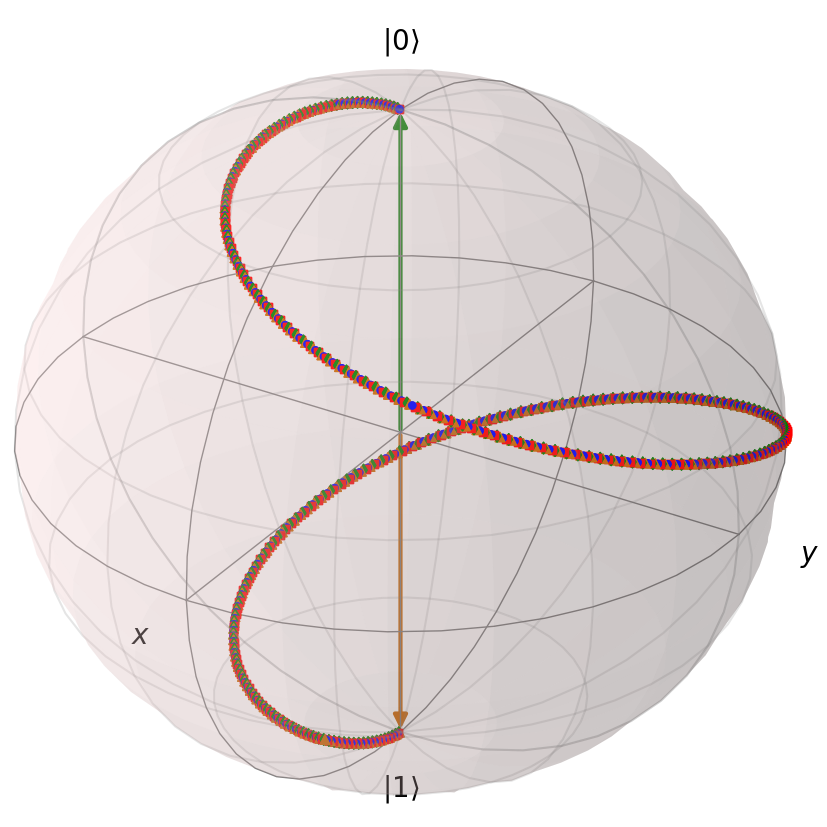
\includegraphics[width=0.4\columnwidth]{Results/qubit-band-amp-const/Bloch-qubit.png}
    \caption{Path of the qubit along the Bloch sphere. The qubit goes from state $\ket{0}$ to state $\ket{1}$, preforming one loop on the sphere, the arrows represent the initial state and the target state, and the points represent the path of the state of the qubit}
    \label{fig:band-amp-const-blcoh}
\end{figure}
As you can see, the path of the qubit isn't a straight line, but some loop, completing a full rotation around the $\hat{z}$ axis. This is explained by the fact that the base Hamiltonian of the qubit is $\omega \hat{\sigma}_z$, where $\hat{\sigma}_z$ is the Pauli matrix Z. This matrix corresponds to rotation of the Bloch sphere around the $\hat{z}$ axis. This is why we can think of the entire Bloch sphere as always rotating with frequency $\omega_0$ around the $\hat{z}$ axis, this is why a "straight" path is actually one that does one loop around the $\hat{z}$ axis.

\subsection{Limiting Pulse Duration}
As much as I wouldn't mind waiting a few nanoseconds longer for the qubit operation to end, the qubit itself isn't as patient as me. A state-of-the-art qubit would last, at most, few hundred microseconds (and that's a very optimistic estimation). We simply don't have the time to wait for the operation to end if we want to run some complicated quantum circuit. This is why we want to add a constraint on the \textit{duration} of the pulse. This way, if we set the total duration of the pulse to longer than the shortest possible pulse, it would find the shorter pulse and the rest of the pulse will change nothing (see figure \ref{fig:dur-penelty})

% give the pulse 5ns to finish, and a solution of 3ns exists, the optimization algorithm would (hopefully) find the 3ns solution and the rest of the time until the end of the duration will do nothing.

The constraint is fairly straight forward, add a penalty for any time a fidelity of 1 isn't achieved. Put into an equation we get
\[
    g_{dur} = \sum_{i = 0}^{N-1} (1 - \mathcal{F}_i)
\]
Where $\mathcal{F}_i$ is the fidelity at time step $i$.

We can rather simply calculate the fidelity at any given time since they are already calculated in order to find the fidelity in the last time step. We can simply modify the loop that calculates the final state into giving the fidelity at each time step and sum the results. 
% TODO: Maybe remove some of the technical details about the code and the implementation

Luckily for us, the calculation of the gradient is also pretty simple. The gradient of the fidelity at each time step is calculated the same as the gradient of the fidelity we calculated in the beginning of the chapter\footnote{note that $\epsilon_k$ only appears in the expression for $\mathcal{F}_i$, if $i > k$, so the sum starts at $i = k$}
\[
    \frac{\partial g_{dur}}{\partial \epsilon_k} = -\sum_{i = k}^{N-1}\frac{\partial \mathcal{F}_i}{\partial \epsilon_k}
\]
% TODO: I think I can find a more efficient solution, Got to check this in the code and ask serge for his opinion

The pulse duration constraint works nicely to complete the other constraints. Without this constraint, the pulse will "try" to use all it's time to get the result we desire. When running the algorithm without the constraint we can get problems if the duration we gave to the pulse is too long or too short. With this constraint on, we can simply give the algorithm a duration that we know for sure is more then the minimum required time, and the algorithm will simply use the minimum time it needs, and no more. On the other hand, if we didn't have the amplitude (and bandwidth) constraints, the algorithm might find that it's best to just give a super-strong pulse for a tiny amount of time, but that's not physically possible as we discussed. This is why we can think of the constraints working together to "box in" the pulse into an ideal "size".

If we run GRAPE now, with all the constraints together, and look at the population of all the level over the duration of the pulse, we get\footnote{This is a rather extreme case where the total duration of the pulse is around three times longer then the minimum duration. This was done purposefully to demonstrate the point.}
% \begin{figure}[H]
%     \centering
%     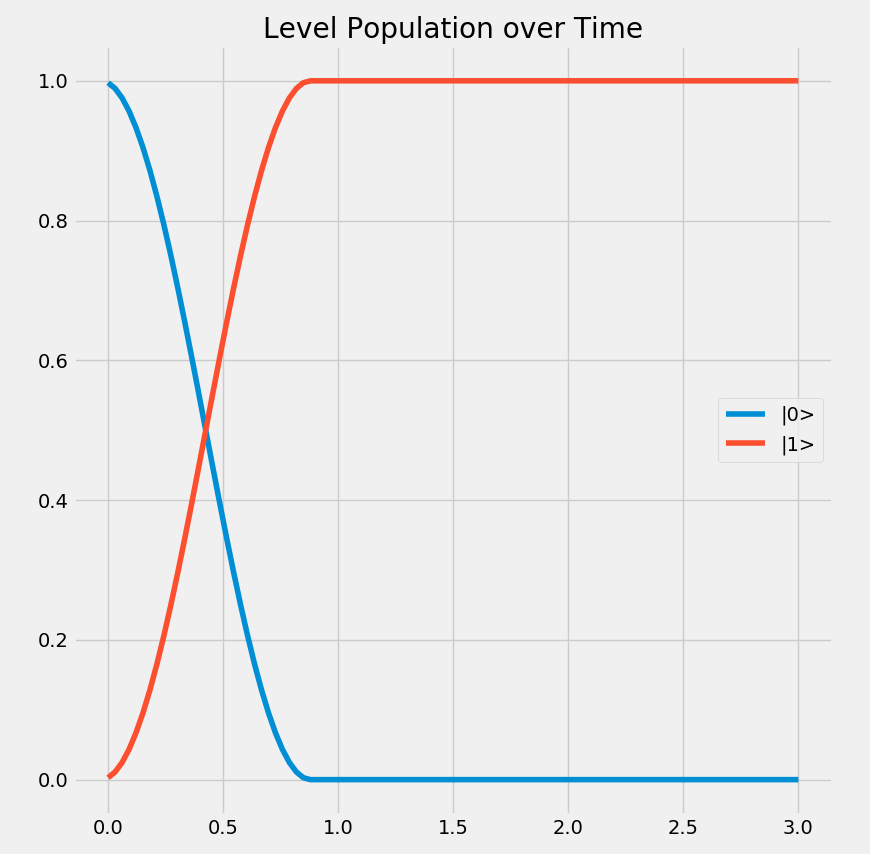
\includegraphics[width=0.5\columnwidth]{Results/duration-constraint/level-population.png}
%     \caption{Level population of each state as a function of time over the duration of the pulse.}
%     \label{fig:dur-penelty}
% \end{figure}
\begin{figure}[H]
    \begin{center}
        %% Creator: Matplotlib, PGF backend
%%
%% To include the figure in your LaTeX document, write
%%   \input{<filename>.pgf}
%%
%% Make sure the required packages are loaded in your preamble
%%   \usepackage{pgf}
%%
%% and, on pdftex
%%   \usepackage[utf8]{inputenc}\DeclareUnicodeCharacter{2212}{-}
%%
%% or, on luatex and xetex
%%   \usepackage{unicode-math}
%%
%% Figures using additional raster images can only be included by \input if
%% they are in the same directory as the main LaTeX file. For loading figures
%% from other directories you can use the `import` package
%%   \usepackage{import}
%%
%% and then include the figures with
%%   \import{<path to file>}{<filename>.pgf}
%%
%% Matplotlib used the following preamble
%%
\begingroup%
\makeatletter%
\begin{pgfpicture}%
\pgfpathrectangle{\pgfpointorigin}{\pgfqpoint{4.650000in}{2.300000in}}%
\pgfusepath{use as bounding box, clip}%
\begin{pgfscope}%
\pgfsetbuttcap%
\pgfsetmiterjoin%
\definecolor{currentfill}{rgb}{1.000000,1.000000,1.000000}%
\pgfsetfillcolor{currentfill}%
\pgfsetlinewidth{0.000000pt}%
\definecolor{currentstroke}{rgb}{1.000000,1.000000,1.000000}%
\pgfsetstrokecolor{currentstroke}%
\pgfsetdash{}{0pt}%
\pgfpathmoveto{\pgfqpoint{0.000000in}{0.000000in}}%
\pgfpathlineto{\pgfqpoint{4.650000in}{0.000000in}}%
\pgfpathlineto{\pgfqpoint{4.650000in}{2.300000in}}%
\pgfpathlineto{\pgfqpoint{0.000000in}{2.300000in}}%
\pgfpathclose%
\pgfusepath{fill}%
\end{pgfscope}%
\begin{pgfscope}%
\pgfsetbuttcap%
\pgfsetmiterjoin%
\definecolor{currentfill}{rgb}{1.000000,1.000000,1.000000}%
\pgfsetfillcolor{currentfill}%
\pgfsetlinewidth{0.000000pt}%
\definecolor{currentstroke}{rgb}{0.000000,0.000000,0.000000}%
\pgfsetstrokecolor{currentstroke}%
\pgfsetstrokeopacity{0.000000}%
\pgfsetdash{}{0pt}%
\pgfpathmoveto{\pgfqpoint{0.646914in}{0.370679in}}%
\pgfpathlineto{\pgfqpoint{2.474152in}{0.370679in}}%
\pgfpathlineto{\pgfqpoint{2.474152in}{1.927778in}}%
\pgfpathlineto{\pgfqpoint{0.646914in}{1.927778in}}%
\pgfpathclose%
\pgfusepath{fill}%
\end{pgfscope}%
\begin{pgfscope}%
\pgfpathrectangle{\pgfqpoint{0.646914in}{0.370679in}}{\pgfqpoint{1.827237in}{1.557099in}}%
\pgfusepath{clip}%
\pgfsetrectcap%
\pgfsetroundjoin%
\pgfsetlinewidth{0.803000pt}%
\definecolor{currentstroke}{rgb}{0.501961,0.501961,0.501961}%
\pgfsetstrokecolor{currentstroke}%
\pgfsetstrokeopacity{0.200000}%
\pgfsetdash{}{0pt}%
\pgfpathmoveto{\pgfqpoint{0.729970in}{0.370679in}}%
\pgfpathlineto{\pgfqpoint{0.729970in}{1.927778in}}%
\pgfusepath{stroke}%
\end{pgfscope}%
\begin{pgfscope}%
\pgfsetbuttcap%
\pgfsetroundjoin%
\definecolor{currentfill}{rgb}{0.333333,0.333333,0.333333}%
\pgfsetfillcolor{currentfill}%
\pgfsetlinewidth{0.803000pt}%
\definecolor{currentstroke}{rgb}{0.333333,0.333333,0.333333}%
\pgfsetstrokecolor{currentstroke}%
\pgfsetdash{}{0pt}%
\pgfsys@defobject{currentmarker}{\pgfqpoint{0.000000in}{-0.048611in}}{\pgfqpoint{0.000000in}{0.000000in}}{%
\pgfpathmoveto{\pgfqpoint{0.000000in}{0.000000in}}%
\pgfpathlineto{\pgfqpoint{0.000000in}{-0.048611in}}%
\pgfusepath{stroke,fill}%
}%
\begin{pgfscope}%
\pgfsys@transformshift{0.729970in}{0.370679in}%
\pgfsys@useobject{currentmarker}{}%
\end{pgfscope}%
\end{pgfscope}%
\begin{pgfscope}%
\definecolor{textcolor}{rgb}{0.333333,0.333333,0.333333}%
\pgfsetstrokecolor{textcolor}%
\pgfsetfillcolor{textcolor}%
\pgftext[x=0.729970in,y=0.273457in,,top]{\color{textcolor}\rmfamily\fontsize{10.000000}{12.000000}\selectfont \(\displaystyle {0}\)}%
\end{pgfscope}%
\begin{pgfscope}%
\pgfpathrectangle{\pgfqpoint{0.646914in}{0.370679in}}{\pgfqpoint{1.827237in}{1.557099in}}%
\pgfusepath{clip}%
\pgfsetrectcap%
\pgfsetroundjoin%
\pgfsetlinewidth{0.803000pt}%
\definecolor{currentstroke}{rgb}{0.501961,0.501961,0.501961}%
\pgfsetstrokecolor{currentstroke}%
\pgfsetstrokeopacity{0.200000}%
\pgfsetdash{}{0pt}%
\pgfpathmoveto{\pgfqpoint{1.394420in}{0.370679in}}%
\pgfpathlineto{\pgfqpoint{1.394420in}{1.927778in}}%
\pgfusepath{stroke}%
\end{pgfscope}%
\begin{pgfscope}%
\pgfsetbuttcap%
\pgfsetroundjoin%
\definecolor{currentfill}{rgb}{0.333333,0.333333,0.333333}%
\pgfsetfillcolor{currentfill}%
\pgfsetlinewidth{0.803000pt}%
\definecolor{currentstroke}{rgb}{0.333333,0.333333,0.333333}%
\pgfsetstrokecolor{currentstroke}%
\pgfsetdash{}{0pt}%
\pgfsys@defobject{currentmarker}{\pgfqpoint{0.000000in}{-0.048611in}}{\pgfqpoint{0.000000in}{0.000000in}}{%
\pgfpathmoveto{\pgfqpoint{0.000000in}{0.000000in}}%
\pgfpathlineto{\pgfqpoint{0.000000in}{-0.048611in}}%
\pgfusepath{stroke,fill}%
}%
\begin{pgfscope}%
\pgfsys@transformshift{1.394420in}{0.370679in}%
\pgfsys@useobject{currentmarker}{}%
\end{pgfscope}%
\end{pgfscope}%
\begin{pgfscope}%
\definecolor{textcolor}{rgb}{0.333333,0.333333,0.333333}%
\pgfsetstrokecolor{textcolor}%
\pgfsetfillcolor{textcolor}%
\pgftext[x=1.394420in,y=0.273457in,,top]{\color{textcolor}\rmfamily\fontsize{10.000000}{12.000000}\selectfont \(\displaystyle {10}\)}%
\end{pgfscope}%
\begin{pgfscope}%
\pgfpathrectangle{\pgfqpoint{0.646914in}{0.370679in}}{\pgfqpoint{1.827237in}{1.557099in}}%
\pgfusepath{clip}%
\pgfsetrectcap%
\pgfsetroundjoin%
\pgfsetlinewidth{0.803000pt}%
\definecolor{currentstroke}{rgb}{0.501961,0.501961,0.501961}%
\pgfsetstrokecolor{currentstroke}%
\pgfsetstrokeopacity{0.200000}%
\pgfsetdash{}{0pt}%
\pgfpathmoveto{\pgfqpoint{2.058870in}{0.370679in}}%
\pgfpathlineto{\pgfqpoint{2.058870in}{1.927778in}}%
\pgfusepath{stroke}%
\end{pgfscope}%
\begin{pgfscope}%
\pgfsetbuttcap%
\pgfsetroundjoin%
\definecolor{currentfill}{rgb}{0.333333,0.333333,0.333333}%
\pgfsetfillcolor{currentfill}%
\pgfsetlinewidth{0.803000pt}%
\definecolor{currentstroke}{rgb}{0.333333,0.333333,0.333333}%
\pgfsetstrokecolor{currentstroke}%
\pgfsetdash{}{0pt}%
\pgfsys@defobject{currentmarker}{\pgfqpoint{0.000000in}{-0.048611in}}{\pgfqpoint{0.000000in}{0.000000in}}{%
\pgfpathmoveto{\pgfqpoint{0.000000in}{0.000000in}}%
\pgfpathlineto{\pgfqpoint{0.000000in}{-0.048611in}}%
\pgfusepath{stroke,fill}%
}%
\begin{pgfscope}%
\pgfsys@transformshift{2.058870in}{0.370679in}%
\pgfsys@useobject{currentmarker}{}%
\end{pgfscope}%
\end{pgfscope}%
\begin{pgfscope}%
\definecolor{textcolor}{rgb}{0.333333,0.333333,0.333333}%
\pgfsetstrokecolor{textcolor}%
\pgfsetfillcolor{textcolor}%
\pgftext[x=2.058870in,y=0.273457in,,top]{\color{textcolor}\rmfamily\fontsize{10.000000}{12.000000}\selectfont \(\displaystyle {20}\)}%
\end{pgfscope}%
\begin{pgfscope}%
\pgfpathrectangle{\pgfqpoint{0.646914in}{0.370679in}}{\pgfqpoint{1.827237in}{1.557099in}}%
\pgfusepath{clip}%
\pgfsetrectcap%
\pgfsetroundjoin%
\pgfsetlinewidth{0.803000pt}%
\definecolor{currentstroke}{rgb}{0.501961,0.501961,0.501961}%
\pgfsetstrokecolor{currentstroke}%
\pgfsetstrokeopacity{0.200000}%
\pgfsetdash{}{0pt}%
\pgfpathmoveto{\pgfqpoint{0.646914in}{0.441456in}}%
\pgfpathlineto{\pgfqpoint{2.474152in}{0.441456in}}%
\pgfusepath{stroke}%
\end{pgfscope}%
\begin{pgfscope}%
\pgfsetbuttcap%
\pgfsetroundjoin%
\definecolor{currentfill}{rgb}{0.333333,0.333333,0.333333}%
\pgfsetfillcolor{currentfill}%
\pgfsetlinewidth{0.803000pt}%
\definecolor{currentstroke}{rgb}{0.333333,0.333333,0.333333}%
\pgfsetstrokecolor{currentstroke}%
\pgfsetdash{}{0pt}%
\pgfsys@defobject{currentmarker}{\pgfqpoint{-0.048611in}{0.000000in}}{\pgfqpoint{0.000000in}{0.000000in}}{%
\pgfpathmoveto{\pgfqpoint{0.000000in}{0.000000in}}%
\pgfpathlineto{\pgfqpoint{-0.048611in}{0.000000in}}%
\pgfusepath{stroke,fill}%
}%
\begin{pgfscope}%
\pgfsys@transformshift{0.646914in}{0.441456in}%
\pgfsys@useobject{currentmarker}{}%
\end{pgfscope}%
\end{pgfscope}%
\begin{pgfscope}%
\definecolor{textcolor}{rgb}{0.333333,0.333333,0.333333}%
\pgfsetstrokecolor{textcolor}%
\pgfsetfillcolor{textcolor}%
\pgftext[x=0.302778in, y=0.393231in, left, base]{\color{textcolor}\rmfamily\fontsize{10.000000}{12.000000}\selectfont \(\displaystyle {0.00}\)}%
\end{pgfscope}%
\begin{pgfscope}%
\pgfpathrectangle{\pgfqpoint{0.646914in}{0.370679in}}{\pgfqpoint{1.827237in}{1.557099in}}%
\pgfusepath{clip}%
\pgfsetrectcap%
\pgfsetroundjoin%
\pgfsetlinewidth{0.803000pt}%
\definecolor{currentstroke}{rgb}{0.501961,0.501961,0.501961}%
\pgfsetstrokecolor{currentstroke}%
\pgfsetstrokeopacity{0.200000}%
\pgfsetdash{}{0pt}%
\pgfpathmoveto{\pgfqpoint{0.646914in}{0.795342in}}%
\pgfpathlineto{\pgfqpoint{2.474152in}{0.795342in}}%
\pgfusepath{stroke}%
\end{pgfscope}%
\begin{pgfscope}%
\pgfsetbuttcap%
\pgfsetroundjoin%
\definecolor{currentfill}{rgb}{0.333333,0.333333,0.333333}%
\pgfsetfillcolor{currentfill}%
\pgfsetlinewidth{0.803000pt}%
\definecolor{currentstroke}{rgb}{0.333333,0.333333,0.333333}%
\pgfsetstrokecolor{currentstroke}%
\pgfsetdash{}{0pt}%
\pgfsys@defobject{currentmarker}{\pgfqpoint{-0.048611in}{0.000000in}}{\pgfqpoint{0.000000in}{0.000000in}}{%
\pgfpathmoveto{\pgfqpoint{0.000000in}{0.000000in}}%
\pgfpathlineto{\pgfqpoint{-0.048611in}{0.000000in}}%
\pgfusepath{stroke,fill}%
}%
\begin{pgfscope}%
\pgfsys@transformshift{0.646914in}{0.795342in}%
\pgfsys@useobject{currentmarker}{}%
\end{pgfscope}%
\end{pgfscope}%
\begin{pgfscope}%
\definecolor{textcolor}{rgb}{0.333333,0.333333,0.333333}%
\pgfsetstrokecolor{textcolor}%
\pgfsetfillcolor{textcolor}%
\pgftext[x=0.302778in, y=0.747117in, left, base]{\color{textcolor}\rmfamily\fontsize{10.000000}{12.000000}\selectfont \(\displaystyle {0.25}\)}%
\end{pgfscope}%
\begin{pgfscope}%
\pgfpathrectangle{\pgfqpoint{0.646914in}{0.370679in}}{\pgfqpoint{1.827237in}{1.557099in}}%
\pgfusepath{clip}%
\pgfsetrectcap%
\pgfsetroundjoin%
\pgfsetlinewidth{0.803000pt}%
\definecolor{currentstroke}{rgb}{0.501961,0.501961,0.501961}%
\pgfsetstrokecolor{currentstroke}%
\pgfsetstrokeopacity{0.200000}%
\pgfsetdash{}{0pt}%
\pgfpathmoveto{\pgfqpoint{0.646914in}{1.149228in}}%
\pgfpathlineto{\pgfqpoint{2.474152in}{1.149228in}}%
\pgfusepath{stroke}%
\end{pgfscope}%
\begin{pgfscope}%
\pgfsetbuttcap%
\pgfsetroundjoin%
\definecolor{currentfill}{rgb}{0.333333,0.333333,0.333333}%
\pgfsetfillcolor{currentfill}%
\pgfsetlinewidth{0.803000pt}%
\definecolor{currentstroke}{rgb}{0.333333,0.333333,0.333333}%
\pgfsetstrokecolor{currentstroke}%
\pgfsetdash{}{0pt}%
\pgfsys@defobject{currentmarker}{\pgfqpoint{-0.048611in}{0.000000in}}{\pgfqpoint{0.000000in}{0.000000in}}{%
\pgfpathmoveto{\pgfqpoint{0.000000in}{0.000000in}}%
\pgfpathlineto{\pgfqpoint{-0.048611in}{0.000000in}}%
\pgfusepath{stroke,fill}%
}%
\begin{pgfscope}%
\pgfsys@transformshift{0.646914in}{1.149228in}%
\pgfsys@useobject{currentmarker}{}%
\end{pgfscope}%
\end{pgfscope}%
\begin{pgfscope}%
\definecolor{textcolor}{rgb}{0.333333,0.333333,0.333333}%
\pgfsetstrokecolor{textcolor}%
\pgfsetfillcolor{textcolor}%
\pgftext[x=0.302778in, y=1.101003in, left, base]{\color{textcolor}\rmfamily\fontsize{10.000000}{12.000000}\selectfont \(\displaystyle {0.50}\)}%
\end{pgfscope}%
\begin{pgfscope}%
\pgfpathrectangle{\pgfqpoint{0.646914in}{0.370679in}}{\pgfqpoint{1.827237in}{1.557099in}}%
\pgfusepath{clip}%
\pgfsetrectcap%
\pgfsetroundjoin%
\pgfsetlinewidth{0.803000pt}%
\definecolor{currentstroke}{rgb}{0.501961,0.501961,0.501961}%
\pgfsetstrokecolor{currentstroke}%
\pgfsetstrokeopacity{0.200000}%
\pgfsetdash{}{0pt}%
\pgfpathmoveto{\pgfqpoint{0.646914in}{1.503115in}}%
\pgfpathlineto{\pgfqpoint{2.474152in}{1.503115in}}%
\pgfusepath{stroke}%
\end{pgfscope}%
\begin{pgfscope}%
\pgfsetbuttcap%
\pgfsetroundjoin%
\definecolor{currentfill}{rgb}{0.333333,0.333333,0.333333}%
\pgfsetfillcolor{currentfill}%
\pgfsetlinewidth{0.803000pt}%
\definecolor{currentstroke}{rgb}{0.333333,0.333333,0.333333}%
\pgfsetstrokecolor{currentstroke}%
\pgfsetdash{}{0pt}%
\pgfsys@defobject{currentmarker}{\pgfqpoint{-0.048611in}{0.000000in}}{\pgfqpoint{0.000000in}{0.000000in}}{%
\pgfpathmoveto{\pgfqpoint{0.000000in}{0.000000in}}%
\pgfpathlineto{\pgfqpoint{-0.048611in}{0.000000in}}%
\pgfusepath{stroke,fill}%
}%
\begin{pgfscope}%
\pgfsys@transformshift{0.646914in}{1.503115in}%
\pgfsys@useobject{currentmarker}{}%
\end{pgfscope}%
\end{pgfscope}%
\begin{pgfscope}%
\definecolor{textcolor}{rgb}{0.333333,0.333333,0.333333}%
\pgfsetstrokecolor{textcolor}%
\pgfsetfillcolor{textcolor}%
\pgftext[x=0.302778in, y=1.454889in, left, base]{\color{textcolor}\rmfamily\fontsize{10.000000}{12.000000}\selectfont \(\displaystyle {0.75}\)}%
\end{pgfscope}%
\begin{pgfscope}%
\pgfpathrectangle{\pgfqpoint{0.646914in}{0.370679in}}{\pgfqpoint{1.827237in}{1.557099in}}%
\pgfusepath{clip}%
\pgfsetrectcap%
\pgfsetroundjoin%
\pgfsetlinewidth{0.803000pt}%
\definecolor{currentstroke}{rgb}{0.501961,0.501961,0.501961}%
\pgfsetstrokecolor{currentstroke}%
\pgfsetstrokeopacity{0.200000}%
\pgfsetdash{}{0pt}%
\pgfpathmoveto{\pgfqpoint{0.646914in}{1.857001in}}%
\pgfpathlineto{\pgfqpoint{2.474152in}{1.857001in}}%
\pgfusepath{stroke}%
\end{pgfscope}%
\begin{pgfscope}%
\pgfsetbuttcap%
\pgfsetroundjoin%
\definecolor{currentfill}{rgb}{0.333333,0.333333,0.333333}%
\pgfsetfillcolor{currentfill}%
\pgfsetlinewidth{0.803000pt}%
\definecolor{currentstroke}{rgb}{0.333333,0.333333,0.333333}%
\pgfsetstrokecolor{currentstroke}%
\pgfsetdash{}{0pt}%
\pgfsys@defobject{currentmarker}{\pgfqpoint{-0.048611in}{0.000000in}}{\pgfqpoint{0.000000in}{0.000000in}}{%
\pgfpathmoveto{\pgfqpoint{0.000000in}{0.000000in}}%
\pgfpathlineto{\pgfqpoint{-0.048611in}{0.000000in}}%
\pgfusepath{stroke,fill}%
}%
\begin{pgfscope}%
\pgfsys@transformshift{0.646914in}{1.857001in}%
\pgfsys@useobject{currentmarker}{}%
\end{pgfscope}%
\end{pgfscope}%
\begin{pgfscope}%
\definecolor{textcolor}{rgb}{0.333333,0.333333,0.333333}%
\pgfsetstrokecolor{textcolor}%
\pgfsetfillcolor{textcolor}%
\pgftext[x=0.302778in, y=1.808776in, left, base]{\color{textcolor}\rmfamily\fontsize{10.000000}{12.000000}\selectfont \(\displaystyle {1.00}\)}%
\end{pgfscope}%
\begin{pgfscope}%
\definecolor{textcolor}{rgb}{0.333333,0.333333,0.333333}%
\pgfsetstrokecolor{textcolor}%
\pgfsetfillcolor{textcolor}%
\pgftext[x=0.247222in,y=1.149228in,,bottom,rotate=90.000000]{\color{textcolor}\rmfamily\fontsize{12.000000}{14.400000}\selectfont Amplitude (MHz)}%
\end{pgfscope}%
\begin{pgfscope}%
\pgfpathrectangle{\pgfqpoint{0.646914in}{0.370679in}}{\pgfqpoint{1.827237in}{1.557099in}}%
\pgfusepath{clip}%
\pgfsetrectcap%
\pgfsetroundjoin%
\pgfsetlinewidth{1.505625pt}%
\definecolor{currentstroke}{rgb}{0.886275,0.290196,0.200000}%
\pgfsetstrokecolor{currentstroke}%
\pgfsetdash{}{0pt}%
\pgfpathmoveto{\pgfqpoint{0.729970in}{1.857001in}}%
\pgfpathlineto{\pgfqpoint{2.391095in}{1.856987in}}%
\pgfpathlineto{\pgfqpoint{2.391095in}{1.856987in}}%
\pgfusepath{stroke}%
\end{pgfscope}%
\begin{pgfscope}%
\pgfpathrectangle{\pgfqpoint{0.646914in}{0.370679in}}{\pgfqpoint{1.827237in}{1.557099in}}%
\pgfusepath{clip}%
\pgfsetrectcap%
\pgfsetroundjoin%
\pgfsetlinewidth{1.505625pt}%
\definecolor{currentstroke}{rgb}{0.203922,0.541176,0.741176}%
\pgfsetstrokecolor{currentstroke}%
\pgfsetdash{}{0pt}%
\pgfpathmoveto{\pgfqpoint{0.729970in}{0.441456in}}%
\pgfpathlineto{\pgfqpoint{2.391095in}{0.441469in}}%
\pgfpathlineto{\pgfqpoint{2.391095in}{0.441469in}}%
\pgfusepath{stroke}%
\end{pgfscope}%
\begin{pgfscope}%
\pgfsetrectcap%
\pgfsetmiterjoin%
\pgfsetlinewidth{1.003750pt}%
\definecolor{currentstroke}{rgb}{1.000000,1.000000,1.000000}%
\pgfsetstrokecolor{currentstroke}%
\pgfsetdash{}{0pt}%
\pgfpathmoveto{\pgfqpoint{0.646914in}{0.370679in}}%
\pgfpathlineto{\pgfqpoint{0.646914in}{1.927778in}}%
\pgfusepath{stroke}%
\end{pgfscope}%
\begin{pgfscope}%
\pgfsetrectcap%
\pgfsetmiterjoin%
\pgfsetlinewidth{1.003750pt}%
\definecolor{currentstroke}{rgb}{1.000000,1.000000,1.000000}%
\pgfsetstrokecolor{currentstroke}%
\pgfsetdash{}{0pt}%
\pgfpathmoveto{\pgfqpoint{2.474152in}{0.370679in}}%
\pgfpathlineto{\pgfqpoint{2.474152in}{1.927778in}}%
\pgfusepath{stroke}%
\end{pgfscope}%
\begin{pgfscope}%
\pgfsetrectcap%
\pgfsetmiterjoin%
\pgfsetlinewidth{1.003750pt}%
\definecolor{currentstroke}{rgb}{1.000000,1.000000,1.000000}%
\pgfsetstrokecolor{currentstroke}%
\pgfsetdash{}{0pt}%
\pgfpathmoveto{\pgfqpoint{0.646914in}{0.370679in}}%
\pgfpathlineto{\pgfqpoint{2.474152in}{0.370679in}}%
\pgfusepath{stroke}%
\end{pgfscope}%
\begin{pgfscope}%
\pgfsetrectcap%
\pgfsetmiterjoin%
\pgfsetlinewidth{1.003750pt}%
\definecolor{currentstroke}{rgb}{1.000000,1.000000,1.000000}%
\pgfsetstrokecolor{currentstroke}%
\pgfsetdash{}{0pt}%
\pgfpathmoveto{\pgfqpoint{0.646914in}{1.927778in}}%
\pgfpathlineto{\pgfqpoint{2.474152in}{1.927778in}}%
\pgfusepath{stroke}%
\end{pgfscope}%
\begin{pgfscope}%
\definecolor{textcolor}{rgb}{0.000000,0.000000,0.000000}%
\pgfsetstrokecolor{textcolor}%
\pgfsetfillcolor{textcolor}%
\pgftext[x=1.560533in,y=2.011111in,,base]{\color{textcolor}\rmfamily\fontsize{14.400000}{17.280000}\selectfont Initial pulse}%
\end{pgfscope}%
\begin{pgfscope}%
\pgfsetbuttcap%
\pgfsetmiterjoin%
\definecolor{currentfill}{rgb}{1.000000,1.000000,1.000000}%
\pgfsetfillcolor{currentfill}%
\pgfsetfillopacity{0.800000}%
\pgfsetlinewidth{0.501875pt}%
\definecolor{currentstroke}{rgb}{0.800000,0.800000,0.800000}%
\pgfsetstrokecolor{currentstroke}%
\pgfsetstrokeopacity{0.800000}%
\pgfsetdash{}{0pt}%
\pgfpathmoveto{\pgfqpoint{1.552179in}{0.920062in}}%
\pgfpathlineto{\pgfqpoint{2.376929in}{0.920062in}}%
\pgfpathquadraticcurveto{\pgfqpoint{2.404707in}{0.920062in}}{\pgfqpoint{2.404707in}{0.947840in}}%
\pgfpathlineto{\pgfqpoint{2.404707in}{1.350617in}}%
\pgfpathquadraticcurveto{\pgfqpoint{2.404707in}{1.378395in}}{\pgfqpoint{2.376929in}{1.378395in}}%
\pgfpathlineto{\pgfqpoint{1.552179in}{1.378395in}}%
\pgfpathquadraticcurveto{\pgfqpoint{1.524402in}{1.378395in}}{\pgfqpoint{1.524402in}{1.350617in}}%
\pgfpathlineto{\pgfqpoint{1.524402in}{0.947840in}}%
\pgfpathquadraticcurveto{\pgfqpoint{1.524402in}{0.920062in}}{\pgfqpoint{1.552179in}{0.920062in}}%
\pgfpathclose%
\pgfusepath{stroke,fill}%
\end{pgfscope}%
\begin{pgfscope}%
\pgfsetrectcap%
\pgfsetroundjoin%
\pgfsetlinewidth{1.505625pt}%
\definecolor{currentstroke}{rgb}{0.886275,0.290196,0.200000}%
\pgfsetstrokecolor{currentstroke}%
\pgfsetdash{}{0pt}%
\pgfpathmoveto{\pgfqpoint{1.579957in}{1.267284in}}%
\pgfpathlineto{\pgfqpoint{1.857735in}{1.267284in}}%
\pgfusepath{stroke}%
\end{pgfscope}%
\begin{pgfscope}%
\definecolor{textcolor}{rgb}{0.000000,0.000000,0.000000}%
\pgfsetstrokecolor{textcolor}%
\pgfsetfillcolor{textcolor}%
\pgftext[x=1.968846in,y=1.218673in,left,base]{\color{textcolor}\rmfamily\fontsize{10.000000}{12.000000}\selectfont \(\displaystyle P(|g\rangle)\)}%
\end{pgfscope}%
\begin{pgfscope}%
\pgfsetrectcap%
\pgfsetroundjoin%
\pgfsetlinewidth{1.505625pt}%
\definecolor{currentstroke}{rgb}{0.203922,0.541176,0.741176}%
\pgfsetstrokecolor{currentstroke}%
\pgfsetdash{}{0pt}%
\pgfpathmoveto{\pgfqpoint{1.579957in}{1.058951in}}%
\pgfpathlineto{\pgfqpoint{1.857735in}{1.058951in}}%
\pgfusepath{stroke}%
\end{pgfscope}%
\begin{pgfscope}%
\definecolor{textcolor}{rgb}{0.000000,0.000000,0.000000}%
\pgfsetstrokecolor{textcolor}%
\pgfsetfillcolor{textcolor}%
\pgftext[x=1.968846in,y=1.010340in,left,base]{\color{textcolor}\rmfamily\fontsize{10.000000}{12.000000}\selectfont \(\displaystyle P(|e\rangle)\)}%
\end{pgfscope}%
\begin{pgfscope}%
\pgfsetbuttcap%
\pgfsetmiterjoin%
\definecolor{currentfill}{rgb}{1.000000,1.000000,1.000000}%
\pgfsetfillcolor{currentfill}%
\pgfsetlinewidth{0.000000pt}%
\definecolor{currentstroke}{rgb}{0.000000,0.000000,0.000000}%
\pgfsetstrokecolor{currentstroke}%
\pgfsetstrokeopacity{0.000000}%
\pgfsetdash{}{0pt}%
\pgfpathmoveto{\pgfqpoint{2.672763in}{0.370679in}}%
\pgfpathlineto{\pgfqpoint{4.500000in}{0.370679in}}%
\pgfpathlineto{\pgfqpoint{4.500000in}{1.927778in}}%
\pgfpathlineto{\pgfqpoint{2.672763in}{1.927778in}}%
\pgfpathclose%
\pgfusepath{fill}%
\end{pgfscope}%
\begin{pgfscope}%
\pgfpathrectangle{\pgfqpoint{2.672763in}{0.370679in}}{\pgfqpoint{1.827237in}{1.557099in}}%
\pgfusepath{clip}%
\pgfsetrectcap%
\pgfsetroundjoin%
\pgfsetlinewidth{0.803000pt}%
\definecolor{currentstroke}{rgb}{0.501961,0.501961,0.501961}%
\pgfsetstrokecolor{currentstroke}%
\pgfsetstrokeopacity{0.200000}%
\pgfsetdash{}{0pt}%
\pgfpathmoveto{\pgfqpoint{2.755819in}{0.370679in}}%
\pgfpathlineto{\pgfqpoint{2.755819in}{1.927778in}}%
\pgfusepath{stroke}%
\end{pgfscope}%
\begin{pgfscope}%
\pgfsetbuttcap%
\pgfsetroundjoin%
\definecolor{currentfill}{rgb}{0.333333,0.333333,0.333333}%
\pgfsetfillcolor{currentfill}%
\pgfsetlinewidth{0.803000pt}%
\definecolor{currentstroke}{rgb}{0.333333,0.333333,0.333333}%
\pgfsetstrokecolor{currentstroke}%
\pgfsetdash{}{0pt}%
\pgfsys@defobject{currentmarker}{\pgfqpoint{0.000000in}{-0.048611in}}{\pgfqpoint{0.000000in}{0.000000in}}{%
\pgfpathmoveto{\pgfqpoint{0.000000in}{0.000000in}}%
\pgfpathlineto{\pgfqpoint{0.000000in}{-0.048611in}}%
\pgfusepath{stroke,fill}%
}%
\begin{pgfscope}%
\pgfsys@transformshift{2.755819in}{0.370679in}%
\pgfsys@useobject{currentmarker}{}%
\end{pgfscope}%
\end{pgfscope}%
\begin{pgfscope}%
\definecolor{textcolor}{rgb}{0.333333,0.333333,0.333333}%
\pgfsetstrokecolor{textcolor}%
\pgfsetfillcolor{textcolor}%
\pgftext[x=2.755819in,y=0.273457in,,top]{\color{textcolor}\rmfamily\fontsize{10.000000}{12.000000}\selectfont \(\displaystyle {0}\)}%
\end{pgfscope}%
\begin{pgfscope}%
\pgfpathrectangle{\pgfqpoint{2.672763in}{0.370679in}}{\pgfqpoint{1.827237in}{1.557099in}}%
\pgfusepath{clip}%
\pgfsetrectcap%
\pgfsetroundjoin%
\pgfsetlinewidth{0.803000pt}%
\definecolor{currentstroke}{rgb}{0.501961,0.501961,0.501961}%
\pgfsetstrokecolor{currentstroke}%
\pgfsetstrokeopacity{0.200000}%
\pgfsetdash{}{0pt}%
\pgfpathmoveto{\pgfqpoint{3.420269in}{0.370679in}}%
\pgfpathlineto{\pgfqpoint{3.420269in}{1.927778in}}%
\pgfusepath{stroke}%
\end{pgfscope}%
\begin{pgfscope}%
\pgfsetbuttcap%
\pgfsetroundjoin%
\definecolor{currentfill}{rgb}{0.333333,0.333333,0.333333}%
\pgfsetfillcolor{currentfill}%
\pgfsetlinewidth{0.803000pt}%
\definecolor{currentstroke}{rgb}{0.333333,0.333333,0.333333}%
\pgfsetstrokecolor{currentstroke}%
\pgfsetdash{}{0pt}%
\pgfsys@defobject{currentmarker}{\pgfqpoint{0.000000in}{-0.048611in}}{\pgfqpoint{0.000000in}{0.000000in}}{%
\pgfpathmoveto{\pgfqpoint{0.000000in}{0.000000in}}%
\pgfpathlineto{\pgfqpoint{0.000000in}{-0.048611in}}%
\pgfusepath{stroke,fill}%
}%
\begin{pgfscope}%
\pgfsys@transformshift{3.420269in}{0.370679in}%
\pgfsys@useobject{currentmarker}{}%
\end{pgfscope}%
\end{pgfscope}%
\begin{pgfscope}%
\definecolor{textcolor}{rgb}{0.333333,0.333333,0.333333}%
\pgfsetstrokecolor{textcolor}%
\pgfsetfillcolor{textcolor}%
\pgftext[x=3.420269in,y=0.273457in,,top]{\color{textcolor}\rmfamily\fontsize{10.000000}{12.000000}\selectfont \(\displaystyle {10}\)}%
\end{pgfscope}%
\begin{pgfscope}%
\pgfpathrectangle{\pgfqpoint{2.672763in}{0.370679in}}{\pgfqpoint{1.827237in}{1.557099in}}%
\pgfusepath{clip}%
\pgfsetrectcap%
\pgfsetroundjoin%
\pgfsetlinewidth{0.803000pt}%
\definecolor{currentstroke}{rgb}{0.501961,0.501961,0.501961}%
\pgfsetstrokecolor{currentstroke}%
\pgfsetstrokeopacity{0.200000}%
\pgfsetdash{}{0pt}%
\pgfpathmoveto{\pgfqpoint{4.084719in}{0.370679in}}%
\pgfpathlineto{\pgfqpoint{4.084719in}{1.927778in}}%
\pgfusepath{stroke}%
\end{pgfscope}%
\begin{pgfscope}%
\pgfsetbuttcap%
\pgfsetroundjoin%
\definecolor{currentfill}{rgb}{0.333333,0.333333,0.333333}%
\pgfsetfillcolor{currentfill}%
\pgfsetlinewidth{0.803000pt}%
\definecolor{currentstroke}{rgb}{0.333333,0.333333,0.333333}%
\pgfsetstrokecolor{currentstroke}%
\pgfsetdash{}{0pt}%
\pgfsys@defobject{currentmarker}{\pgfqpoint{0.000000in}{-0.048611in}}{\pgfqpoint{0.000000in}{0.000000in}}{%
\pgfpathmoveto{\pgfqpoint{0.000000in}{0.000000in}}%
\pgfpathlineto{\pgfqpoint{0.000000in}{-0.048611in}}%
\pgfusepath{stroke,fill}%
}%
\begin{pgfscope}%
\pgfsys@transformshift{4.084719in}{0.370679in}%
\pgfsys@useobject{currentmarker}{}%
\end{pgfscope}%
\end{pgfscope}%
\begin{pgfscope}%
\definecolor{textcolor}{rgb}{0.333333,0.333333,0.333333}%
\pgfsetstrokecolor{textcolor}%
\pgfsetfillcolor{textcolor}%
\pgftext[x=4.084719in,y=0.273457in,,top]{\color{textcolor}\rmfamily\fontsize{10.000000}{12.000000}\selectfont \(\displaystyle {20}\)}%
\end{pgfscope}%
\begin{pgfscope}%
\pgfpathrectangle{\pgfqpoint{2.672763in}{0.370679in}}{\pgfqpoint{1.827237in}{1.557099in}}%
\pgfusepath{clip}%
\pgfsetrectcap%
\pgfsetroundjoin%
\pgfsetlinewidth{0.803000pt}%
\definecolor{currentstroke}{rgb}{0.501961,0.501961,0.501961}%
\pgfsetstrokecolor{currentstroke}%
\pgfsetstrokeopacity{0.200000}%
\pgfsetdash{}{0pt}%
\pgfpathmoveto{\pgfqpoint{2.672763in}{0.441456in}}%
\pgfpathlineto{\pgfqpoint{4.500000in}{0.441456in}}%
\pgfusepath{stroke}%
\end{pgfscope}%
\begin{pgfscope}%
\pgfsetbuttcap%
\pgfsetroundjoin%
\definecolor{currentfill}{rgb}{0.333333,0.333333,0.333333}%
\pgfsetfillcolor{currentfill}%
\pgfsetlinewidth{0.803000pt}%
\definecolor{currentstroke}{rgb}{0.333333,0.333333,0.333333}%
\pgfsetstrokecolor{currentstroke}%
\pgfsetdash{}{0pt}%
\pgfsys@defobject{currentmarker}{\pgfqpoint{-0.048611in}{0.000000in}}{\pgfqpoint{0.000000in}{0.000000in}}{%
\pgfpathmoveto{\pgfqpoint{0.000000in}{0.000000in}}%
\pgfpathlineto{\pgfqpoint{-0.048611in}{0.000000in}}%
\pgfusepath{stroke,fill}%
}%
\begin{pgfscope}%
\pgfsys@transformshift{2.672763in}{0.441456in}%
\pgfsys@useobject{currentmarker}{}%
\end{pgfscope}%
\end{pgfscope}%
\begin{pgfscope}%
\pgfpathrectangle{\pgfqpoint{2.672763in}{0.370679in}}{\pgfqpoint{1.827237in}{1.557099in}}%
\pgfusepath{clip}%
\pgfsetrectcap%
\pgfsetroundjoin%
\pgfsetlinewidth{0.803000pt}%
\definecolor{currentstroke}{rgb}{0.501961,0.501961,0.501961}%
\pgfsetstrokecolor{currentstroke}%
\pgfsetstrokeopacity{0.200000}%
\pgfsetdash{}{0pt}%
\pgfpathmoveto{\pgfqpoint{2.672763in}{0.795342in}}%
\pgfpathlineto{\pgfqpoint{4.500000in}{0.795342in}}%
\pgfusepath{stroke}%
\end{pgfscope}%
\begin{pgfscope}%
\pgfsetbuttcap%
\pgfsetroundjoin%
\definecolor{currentfill}{rgb}{0.333333,0.333333,0.333333}%
\pgfsetfillcolor{currentfill}%
\pgfsetlinewidth{0.803000pt}%
\definecolor{currentstroke}{rgb}{0.333333,0.333333,0.333333}%
\pgfsetstrokecolor{currentstroke}%
\pgfsetdash{}{0pt}%
\pgfsys@defobject{currentmarker}{\pgfqpoint{-0.048611in}{0.000000in}}{\pgfqpoint{0.000000in}{0.000000in}}{%
\pgfpathmoveto{\pgfqpoint{0.000000in}{0.000000in}}%
\pgfpathlineto{\pgfqpoint{-0.048611in}{0.000000in}}%
\pgfusepath{stroke,fill}%
}%
\begin{pgfscope}%
\pgfsys@transformshift{2.672763in}{0.795342in}%
\pgfsys@useobject{currentmarker}{}%
\end{pgfscope}%
\end{pgfscope}%
\begin{pgfscope}%
\pgfpathrectangle{\pgfqpoint{2.672763in}{0.370679in}}{\pgfqpoint{1.827237in}{1.557099in}}%
\pgfusepath{clip}%
\pgfsetrectcap%
\pgfsetroundjoin%
\pgfsetlinewidth{0.803000pt}%
\definecolor{currentstroke}{rgb}{0.501961,0.501961,0.501961}%
\pgfsetstrokecolor{currentstroke}%
\pgfsetstrokeopacity{0.200000}%
\pgfsetdash{}{0pt}%
\pgfpathmoveto{\pgfqpoint{2.672763in}{1.149228in}}%
\pgfpathlineto{\pgfqpoint{4.500000in}{1.149228in}}%
\pgfusepath{stroke}%
\end{pgfscope}%
\begin{pgfscope}%
\pgfsetbuttcap%
\pgfsetroundjoin%
\definecolor{currentfill}{rgb}{0.333333,0.333333,0.333333}%
\pgfsetfillcolor{currentfill}%
\pgfsetlinewidth{0.803000pt}%
\definecolor{currentstroke}{rgb}{0.333333,0.333333,0.333333}%
\pgfsetstrokecolor{currentstroke}%
\pgfsetdash{}{0pt}%
\pgfsys@defobject{currentmarker}{\pgfqpoint{-0.048611in}{0.000000in}}{\pgfqpoint{0.000000in}{0.000000in}}{%
\pgfpathmoveto{\pgfqpoint{0.000000in}{0.000000in}}%
\pgfpathlineto{\pgfqpoint{-0.048611in}{0.000000in}}%
\pgfusepath{stroke,fill}%
}%
\begin{pgfscope}%
\pgfsys@transformshift{2.672763in}{1.149228in}%
\pgfsys@useobject{currentmarker}{}%
\end{pgfscope}%
\end{pgfscope}%
\begin{pgfscope}%
\pgfpathrectangle{\pgfqpoint{2.672763in}{0.370679in}}{\pgfqpoint{1.827237in}{1.557099in}}%
\pgfusepath{clip}%
\pgfsetrectcap%
\pgfsetroundjoin%
\pgfsetlinewidth{0.803000pt}%
\definecolor{currentstroke}{rgb}{0.501961,0.501961,0.501961}%
\pgfsetstrokecolor{currentstroke}%
\pgfsetstrokeopacity{0.200000}%
\pgfsetdash{}{0pt}%
\pgfpathmoveto{\pgfqpoint{2.672763in}{1.503115in}}%
\pgfpathlineto{\pgfqpoint{4.500000in}{1.503115in}}%
\pgfusepath{stroke}%
\end{pgfscope}%
\begin{pgfscope}%
\pgfsetbuttcap%
\pgfsetroundjoin%
\definecolor{currentfill}{rgb}{0.333333,0.333333,0.333333}%
\pgfsetfillcolor{currentfill}%
\pgfsetlinewidth{0.803000pt}%
\definecolor{currentstroke}{rgb}{0.333333,0.333333,0.333333}%
\pgfsetstrokecolor{currentstroke}%
\pgfsetdash{}{0pt}%
\pgfsys@defobject{currentmarker}{\pgfqpoint{-0.048611in}{0.000000in}}{\pgfqpoint{0.000000in}{0.000000in}}{%
\pgfpathmoveto{\pgfqpoint{0.000000in}{0.000000in}}%
\pgfpathlineto{\pgfqpoint{-0.048611in}{0.000000in}}%
\pgfusepath{stroke,fill}%
}%
\begin{pgfscope}%
\pgfsys@transformshift{2.672763in}{1.503115in}%
\pgfsys@useobject{currentmarker}{}%
\end{pgfscope}%
\end{pgfscope}%
\begin{pgfscope}%
\pgfpathrectangle{\pgfqpoint{2.672763in}{0.370679in}}{\pgfqpoint{1.827237in}{1.557099in}}%
\pgfusepath{clip}%
\pgfsetrectcap%
\pgfsetroundjoin%
\pgfsetlinewidth{0.803000pt}%
\definecolor{currentstroke}{rgb}{0.501961,0.501961,0.501961}%
\pgfsetstrokecolor{currentstroke}%
\pgfsetstrokeopacity{0.200000}%
\pgfsetdash{}{0pt}%
\pgfpathmoveto{\pgfqpoint{2.672763in}{1.857001in}}%
\pgfpathlineto{\pgfqpoint{4.500000in}{1.857001in}}%
\pgfusepath{stroke}%
\end{pgfscope}%
\begin{pgfscope}%
\pgfsetbuttcap%
\pgfsetroundjoin%
\definecolor{currentfill}{rgb}{0.333333,0.333333,0.333333}%
\pgfsetfillcolor{currentfill}%
\pgfsetlinewidth{0.803000pt}%
\definecolor{currentstroke}{rgb}{0.333333,0.333333,0.333333}%
\pgfsetstrokecolor{currentstroke}%
\pgfsetdash{}{0pt}%
\pgfsys@defobject{currentmarker}{\pgfqpoint{-0.048611in}{0.000000in}}{\pgfqpoint{0.000000in}{0.000000in}}{%
\pgfpathmoveto{\pgfqpoint{0.000000in}{0.000000in}}%
\pgfpathlineto{\pgfqpoint{-0.048611in}{0.000000in}}%
\pgfusepath{stroke,fill}%
}%
\begin{pgfscope}%
\pgfsys@transformshift{2.672763in}{1.857001in}%
\pgfsys@useobject{currentmarker}{}%
\end{pgfscope}%
\end{pgfscope}%
\begin{pgfscope}%
\pgfpathrectangle{\pgfqpoint{2.672763in}{0.370679in}}{\pgfqpoint{1.827237in}{1.557099in}}%
\pgfusepath{clip}%
\pgfsetrectcap%
\pgfsetroundjoin%
\pgfsetlinewidth{1.505625pt}%
\definecolor{currentstroke}{rgb}{0.886275,0.290196,0.200000}%
\pgfsetstrokecolor{currentstroke}%
\pgfsetdash{}{0pt}%
\pgfpathmoveto{\pgfqpoint{2.755819in}{1.856915in}}%
\pgfpathlineto{\pgfqpoint{2.789208in}{1.854853in}}%
\pgfpathlineto{\pgfqpoint{2.822598in}{1.849998in}}%
\pgfpathlineto{\pgfqpoint{2.855987in}{1.842205in}}%
\pgfpathlineto{\pgfqpoint{2.889377in}{1.831577in}}%
\pgfpathlineto{\pgfqpoint{2.922766in}{1.818382in}}%
\pgfpathlineto{\pgfqpoint{2.964503in}{1.797995in}}%
\pgfpathlineto{\pgfqpoint{3.006240in}{1.773568in}}%
\pgfpathlineto{\pgfqpoint{3.047977in}{1.745323in}}%
\pgfpathlineto{\pgfqpoint{3.098061in}{1.707292in}}%
\pgfpathlineto{\pgfqpoint{3.148145in}{1.663981in}}%
\pgfpathlineto{\pgfqpoint{3.189882in}{1.624561in}}%
\pgfpathlineto{\pgfqpoint{3.239966in}{1.573058in}}%
\pgfpathlineto{\pgfqpoint{3.298397in}{1.508591in}}%
\pgfpathlineto{\pgfqpoint{3.348482in}{1.449914in}}%
\pgfpathlineto{\pgfqpoint{3.415260in}{1.365946in}}%
\pgfpathlineto{\pgfqpoint{3.565513in}{1.170061in}}%
\pgfpathlineto{\pgfqpoint{3.732460in}{0.950177in}}%
\pgfpathlineto{\pgfqpoint{3.815934in}{0.847804in}}%
\pgfpathlineto{\pgfqpoint{3.891060in}{0.761994in}}%
\pgfpathlineto{\pgfqpoint{3.949492in}{0.699613in}}%
\pgfpathlineto{\pgfqpoint{3.999576in}{0.649561in}}%
\pgfpathlineto{\pgfqpoint{4.049660in}{0.604309in}}%
\pgfpathlineto{\pgfqpoint{4.091397in}{0.570493in}}%
\pgfpathlineto{\pgfqpoint{4.141481in}{0.534391in}}%
\pgfpathlineto{\pgfqpoint{4.183218in}{0.508237in}}%
\pgfpathlineto{\pgfqpoint{4.224954in}{0.486459in}}%
\pgfpathlineto{\pgfqpoint{4.258344in}{0.472265in}}%
\pgfpathlineto{\pgfqpoint{4.300081in}{0.458408in}}%
\pgfpathlineto{\pgfqpoint{4.333470in}{0.450132in}}%
\pgfpathlineto{\pgfqpoint{4.366860in}{0.444555in}}%
\pgfpathlineto{\pgfqpoint{4.400249in}{0.441789in}}%
\pgfpathlineto{\pgfqpoint{4.416944in}{0.441456in}}%
\pgfpathlineto{\pgfqpoint{4.416944in}{0.441456in}}%
\pgfusepath{stroke}%
\end{pgfscope}%
\begin{pgfscope}%
\pgfpathrectangle{\pgfqpoint{2.672763in}{0.370679in}}{\pgfqpoint{1.827237in}{1.557099in}}%
\pgfusepath{clip}%
\pgfsetrectcap%
\pgfsetroundjoin%
\pgfsetlinewidth{1.505625pt}%
\definecolor{currentstroke}{rgb}{0.203922,0.541176,0.741176}%
\pgfsetstrokecolor{currentstroke}%
\pgfsetdash{}{0pt}%
\pgfpathmoveto{\pgfqpoint{2.755819in}{0.441542in}}%
\pgfpathlineto{\pgfqpoint{2.789208in}{0.443604in}}%
\pgfpathlineto{\pgfqpoint{2.822598in}{0.448458in}}%
\pgfpathlineto{\pgfqpoint{2.855987in}{0.456252in}}%
\pgfpathlineto{\pgfqpoint{2.889377in}{0.466880in}}%
\pgfpathlineto{\pgfqpoint{2.922766in}{0.480075in}}%
\pgfpathlineto{\pgfqpoint{2.964503in}{0.500462in}}%
\pgfpathlineto{\pgfqpoint{3.006240in}{0.524888in}}%
\pgfpathlineto{\pgfqpoint{3.047977in}{0.553134in}}%
\pgfpathlineto{\pgfqpoint{3.098061in}{0.591165in}}%
\pgfpathlineto{\pgfqpoint{3.148145in}{0.634476in}}%
\pgfpathlineto{\pgfqpoint{3.189882in}{0.673896in}}%
\pgfpathlineto{\pgfqpoint{3.239966in}{0.725399in}}%
\pgfpathlineto{\pgfqpoint{3.298397in}{0.789866in}}%
\pgfpathlineto{\pgfqpoint{3.348482in}{0.848543in}}%
\pgfpathlineto{\pgfqpoint{3.415260in}{0.932511in}}%
\pgfpathlineto{\pgfqpoint{3.565513in}{1.128396in}}%
\pgfpathlineto{\pgfqpoint{3.732460in}{1.348280in}}%
\pgfpathlineto{\pgfqpoint{3.815934in}{1.450653in}}%
\pgfpathlineto{\pgfqpoint{3.891060in}{1.536463in}}%
\pgfpathlineto{\pgfqpoint{3.949492in}{1.598844in}}%
\pgfpathlineto{\pgfqpoint{3.999576in}{1.648896in}}%
\pgfpathlineto{\pgfqpoint{4.049660in}{1.694148in}}%
\pgfpathlineto{\pgfqpoint{4.091397in}{1.727964in}}%
\pgfpathlineto{\pgfqpoint{4.141481in}{1.764065in}}%
\pgfpathlineto{\pgfqpoint{4.183218in}{1.790220in}}%
\pgfpathlineto{\pgfqpoint{4.224954in}{1.811998in}}%
\pgfpathlineto{\pgfqpoint{4.258344in}{1.826192in}}%
\pgfpathlineto{\pgfqpoint{4.300081in}{1.840049in}}%
\pgfpathlineto{\pgfqpoint{4.333470in}{1.848325in}}%
\pgfpathlineto{\pgfqpoint{4.366860in}{1.853902in}}%
\pgfpathlineto{\pgfqpoint{4.400249in}{1.856668in}}%
\pgfpathlineto{\pgfqpoint{4.416944in}{1.857001in}}%
\pgfpathlineto{\pgfqpoint{4.416944in}{1.857001in}}%
\pgfusepath{stroke}%
\end{pgfscope}%
\begin{pgfscope}%
\pgfsetrectcap%
\pgfsetmiterjoin%
\pgfsetlinewidth{1.003750pt}%
\definecolor{currentstroke}{rgb}{1.000000,1.000000,1.000000}%
\pgfsetstrokecolor{currentstroke}%
\pgfsetdash{}{0pt}%
\pgfpathmoveto{\pgfqpoint{2.672763in}{0.370679in}}%
\pgfpathlineto{\pgfqpoint{2.672763in}{1.927778in}}%
\pgfusepath{stroke}%
\end{pgfscope}%
\begin{pgfscope}%
\pgfsetrectcap%
\pgfsetmiterjoin%
\pgfsetlinewidth{1.003750pt}%
\definecolor{currentstroke}{rgb}{1.000000,1.000000,1.000000}%
\pgfsetstrokecolor{currentstroke}%
\pgfsetdash{}{0pt}%
\pgfpathmoveto{\pgfqpoint{4.500000in}{0.370679in}}%
\pgfpathlineto{\pgfqpoint{4.500000in}{1.927778in}}%
\pgfusepath{stroke}%
\end{pgfscope}%
\begin{pgfscope}%
\pgfsetrectcap%
\pgfsetmiterjoin%
\pgfsetlinewidth{1.003750pt}%
\definecolor{currentstroke}{rgb}{1.000000,1.000000,1.000000}%
\pgfsetstrokecolor{currentstroke}%
\pgfsetdash{}{0pt}%
\pgfpathmoveto{\pgfqpoint{2.672763in}{0.370679in}}%
\pgfpathlineto{\pgfqpoint{4.500000in}{0.370679in}}%
\pgfusepath{stroke}%
\end{pgfscope}%
\begin{pgfscope}%
\pgfsetrectcap%
\pgfsetmiterjoin%
\pgfsetlinewidth{1.003750pt}%
\definecolor{currentstroke}{rgb}{1.000000,1.000000,1.000000}%
\pgfsetstrokecolor{currentstroke}%
\pgfsetdash{}{0pt}%
\pgfpathmoveto{\pgfqpoint{2.672763in}{1.927778in}}%
\pgfpathlineto{\pgfqpoint{4.500000in}{1.927778in}}%
\pgfusepath{stroke}%
\end{pgfscope}%
\begin{pgfscope}%
\definecolor{textcolor}{rgb}{0.000000,0.000000,0.000000}%
\pgfsetstrokecolor{textcolor}%
\pgfsetfillcolor{textcolor}%
\pgftext[x=3.586381in,y=2.011111in,,base]{\color{textcolor}\rmfamily\fontsize{14.400000}{17.280000}\selectfont Final pulse}%
\end{pgfscope}%
\begin{pgfscope}%
\definecolor{textcolor}{rgb}{0.000000,0.000000,0.000000}%
\pgfsetstrokecolor{textcolor}%
\pgfsetfillcolor{textcolor}%
\pgftext[x=2.325000in,y=0.000000in,,base]{\color{textcolor}\rmfamily\fontsize{12.000000}{14.400000}\selectfont Time (ns)}%
\end{pgfscope}%
\end{pgfpicture}%
\makeatother%
\endgroup%

    \end{center}
    \caption{Level population of each state as a function of time over the duration of the pulse.}
    \label{fig:dur-penelty}
\end{figure}

As expected, we get exactly what we want, the pulse uses the least amount of time that it needs and then stop. This way, if we pick a long duration for the pulse, instead of the pulse trying to fill the entire time at a very low amplitude, or do several of loops before arriving at the target, the qubit simply takes exactly the amount of time that it needs to get to the desired state under all of the constraints and then stops.

\section{Implementing Qubit Operations with GRAPE}

\subsection{DRAG - Imperfect Qubits} \label{sec:DRAG}
When we did all of our calculation on the qubit we didn't include one detail, it's really hard to create a true two-level system. In the way our qubits are implemented, there are actually more than two levels. It's not a two level system but we treat it as one. Since the higher levels are off-resonance, we can often just ignore them. However, there is some probability of the higher levels getting populated by high-frequency components of our pulses. The shorter our pulses are, the more these higher  levels excitation occur. We will prevent those so-called leakage errors by using \textbf{D}erivative \textbf{R}emoval via \textbf{A}diabatic \textbf{G}ate (DRAG) pulses. We can generate those pulses by including more than two levels in our algorithm and changing the Hamiltonian a little bit so it accounts for the off-resonance higher levels.

Before we continue to implement DRAG, let's see if the third level really is that much of a problem. We run a simulation of GRAPE just as we did before but this time with three levels instead of two, and the third level should start and end at 0 population. We get after running GRAPE
% \begin{figure}[H]
%     \centering
%     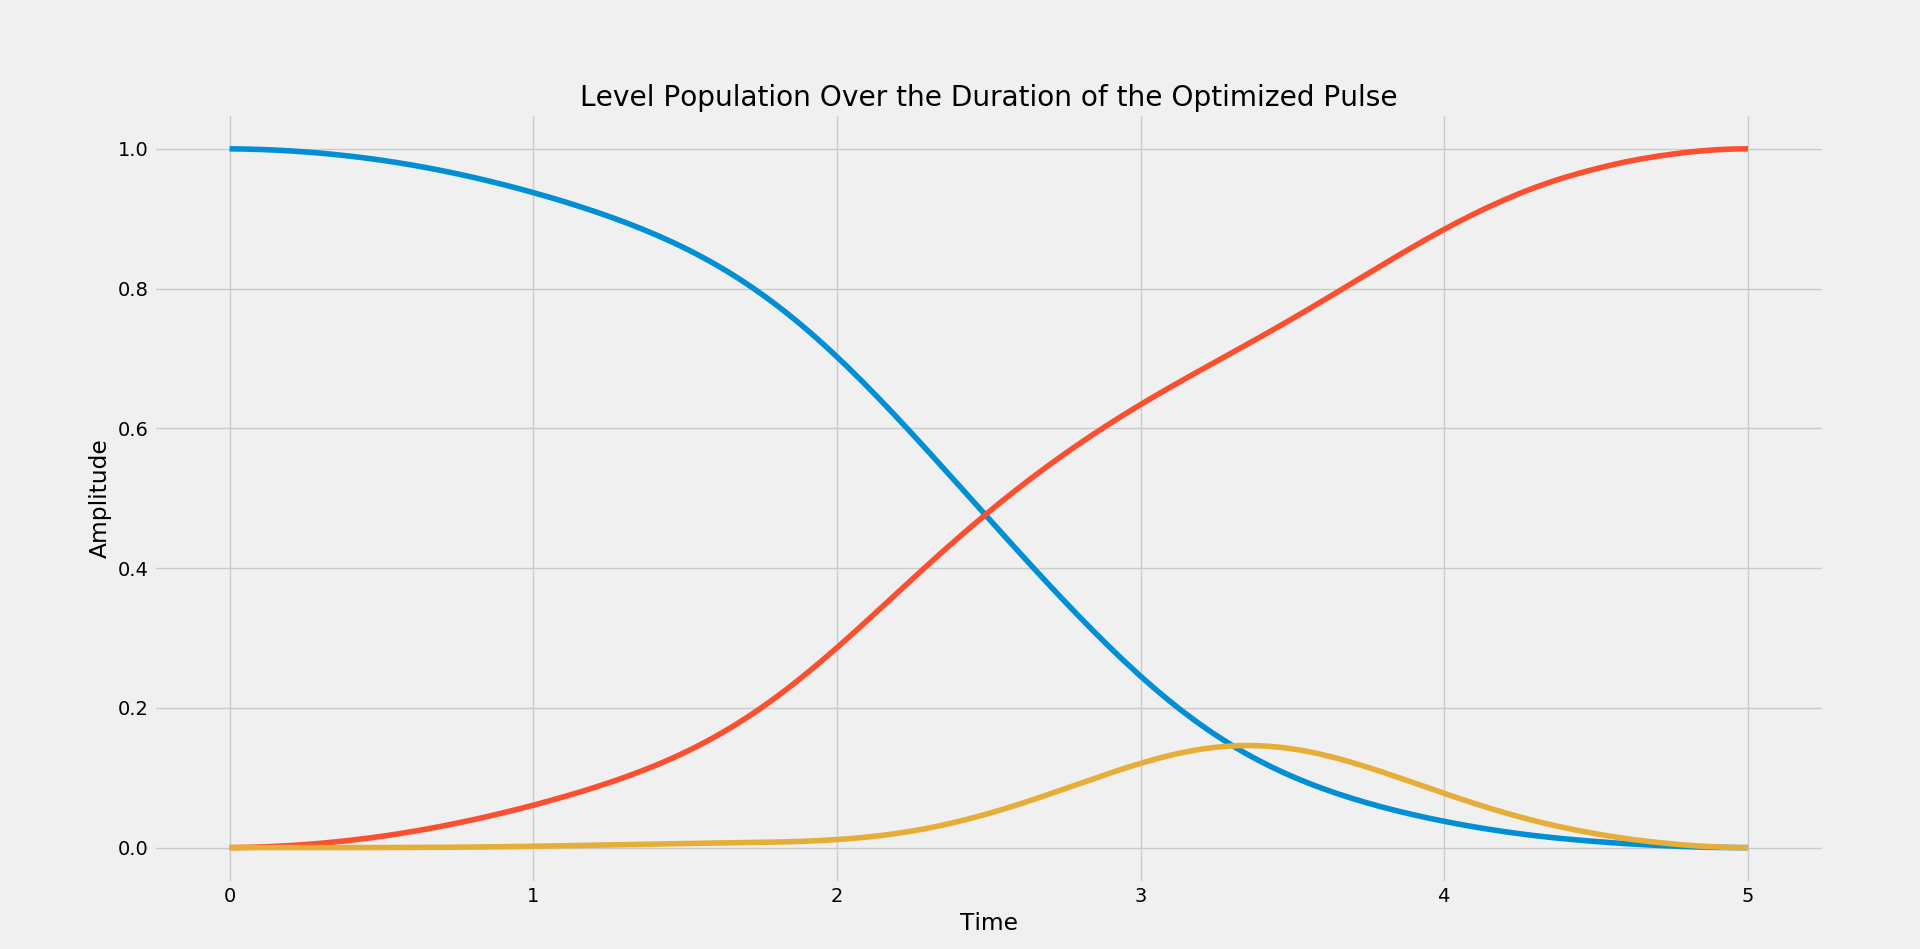
\includegraphics[width=1\columnwidth]{Results/Before-Drag/level-population-pretty.png}
%     \caption{Level population of the 3-level "qubit" over the duration of the pulse calculated by the GRAPE algorithm we have so far}
%     \label{fig:before-DRAG}
% \end{figure}
\begin{figure}[H]
    \begin{center}
        %% Creator: Matplotlib, PGF backend
%%
%% To include the figure in your LaTeX document, write
%%   \input{<filename>.pgf}
%%
%% Make sure the required packages are loaded in your preamble
%%   \usepackage{pgf}
%%
%% and, on pdftex
%%   \usepackage[utf8]{inputenc}\DeclareUnicodeCharacter{2212}{-}
%%
%% or, on luatex and xetex
%%   \usepackage{unicode-math}
%%
%% Figures using additional raster images can only be included by \input if
%% they are in the same directory as the main LaTeX file. For loading figures
%% from other directories you can use the `import` package
%%   \usepackage{import}
%%
%% and then include the figures with
%%   \import{<path to file>}{<filename>.pgf}
%%
%% Matplotlib used the following preamble
%%
\begingroup%
\makeatletter%
\begin{pgfpicture}%
\pgfpathrectangle{\pgfpointorigin}{\pgfqpoint{4.650000in}{2.300000in}}%
\pgfusepath{use as bounding box, clip}%
\begin{pgfscope}%
\pgfsetbuttcap%
\pgfsetmiterjoin%
\definecolor{currentfill}{rgb}{1.000000,1.000000,1.000000}%
\pgfsetfillcolor{currentfill}%
\pgfsetlinewidth{0.000000pt}%
\definecolor{currentstroke}{rgb}{1.000000,1.000000,1.000000}%
\pgfsetstrokecolor{currentstroke}%
\pgfsetdash{}{0pt}%
\pgfpathmoveto{\pgfqpoint{0.000000in}{0.000000in}}%
\pgfpathlineto{\pgfqpoint{4.650000in}{0.000000in}}%
\pgfpathlineto{\pgfqpoint{4.650000in}{2.300000in}}%
\pgfpathlineto{\pgfqpoint{0.000000in}{2.300000in}}%
\pgfpathclose%
\pgfusepath{fill}%
\end{pgfscope}%
\begin{pgfscope}%
\pgfsetbuttcap%
\pgfsetmiterjoin%
\definecolor{currentfill}{rgb}{1.000000,1.000000,1.000000}%
\pgfsetfillcolor{currentfill}%
\pgfsetlinewidth{0.000000pt}%
\definecolor{currentstroke}{rgb}{0.000000,0.000000,0.000000}%
\pgfsetstrokecolor{currentstroke}%
\pgfsetstrokeopacity{0.000000}%
\pgfsetdash{}{0pt}%
\pgfpathmoveto{\pgfqpoint{0.646914in}{0.370679in}}%
\pgfpathlineto{\pgfqpoint{2.474152in}{0.370679in}}%
\pgfpathlineto{\pgfqpoint{2.474152in}{1.927778in}}%
\pgfpathlineto{\pgfqpoint{0.646914in}{1.927778in}}%
\pgfpathclose%
\pgfusepath{fill}%
\end{pgfscope}%
\begin{pgfscope}%
\pgfpathrectangle{\pgfqpoint{0.646914in}{0.370679in}}{\pgfqpoint{1.827237in}{1.557099in}}%
\pgfusepath{clip}%
\pgfsetrectcap%
\pgfsetroundjoin%
\pgfsetlinewidth{0.803000pt}%
\definecolor{currentstroke}{rgb}{0.501961,0.501961,0.501961}%
\pgfsetstrokecolor{currentstroke}%
\pgfsetstrokeopacity{0.200000}%
\pgfsetdash{}{0pt}%
\pgfpathmoveto{\pgfqpoint{0.729970in}{0.370679in}}%
\pgfpathlineto{\pgfqpoint{0.729970in}{1.927778in}}%
\pgfusepath{stroke}%
\end{pgfscope}%
\begin{pgfscope}%
\pgfsetbuttcap%
\pgfsetroundjoin%
\definecolor{currentfill}{rgb}{0.333333,0.333333,0.333333}%
\pgfsetfillcolor{currentfill}%
\pgfsetlinewidth{0.803000pt}%
\definecolor{currentstroke}{rgb}{0.333333,0.333333,0.333333}%
\pgfsetstrokecolor{currentstroke}%
\pgfsetdash{}{0pt}%
\pgfsys@defobject{currentmarker}{\pgfqpoint{0.000000in}{-0.048611in}}{\pgfqpoint{0.000000in}{0.000000in}}{%
\pgfpathmoveto{\pgfqpoint{0.000000in}{0.000000in}}%
\pgfpathlineto{\pgfqpoint{0.000000in}{-0.048611in}}%
\pgfusepath{stroke,fill}%
}%
\begin{pgfscope}%
\pgfsys@transformshift{0.729970in}{0.370679in}%
\pgfsys@useobject{currentmarker}{}%
\end{pgfscope}%
\end{pgfscope}%
\begin{pgfscope}%
\definecolor{textcolor}{rgb}{0.333333,0.333333,0.333333}%
\pgfsetstrokecolor{textcolor}%
\pgfsetfillcolor{textcolor}%
\pgftext[x=0.729970in,y=0.273457in,,top]{\color{textcolor}\rmfamily\fontsize{10.000000}{12.000000}\selectfont \(\displaystyle {0}\)}%
\end{pgfscope}%
\begin{pgfscope}%
\pgfpathrectangle{\pgfqpoint{0.646914in}{0.370679in}}{\pgfqpoint{1.827237in}{1.557099in}}%
\pgfusepath{clip}%
\pgfsetrectcap%
\pgfsetroundjoin%
\pgfsetlinewidth{0.803000pt}%
\definecolor{currentstroke}{rgb}{0.501961,0.501961,0.501961}%
\pgfsetstrokecolor{currentstroke}%
\pgfsetstrokeopacity{0.200000}%
\pgfsetdash{}{0pt}%
\pgfpathmoveto{\pgfqpoint{1.394420in}{0.370679in}}%
\pgfpathlineto{\pgfqpoint{1.394420in}{1.927778in}}%
\pgfusepath{stroke}%
\end{pgfscope}%
\begin{pgfscope}%
\pgfsetbuttcap%
\pgfsetroundjoin%
\definecolor{currentfill}{rgb}{0.333333,0.333333,0.333333}%
\pgfsetfillcolor{currentfill}%
\pgfsetlinewidth{0.803000pt}%
\definecolor{currentstroke}{rgb}{0.333333,0.333333,0.333333}%
\pgfsetstrokecolor{currentstroke}%
\pgfsetdash{}{0pt}%
\pgfsys@defobject{currentmarker}{\pgfqpoint{0.000000in}{-0.048611in}}{\pgfqpoint{0.000000in}{0.000000in}}{%
\pgfpathmoveto{\pgfqpoint{0.000000in}{0.000000in}}%
\pgfpathlineto{\pgfqpoint{0.000000in}{-0.048611in}}%
\pgfusepath{stroke,fill}%
}%
\begin{pgfscope}%
\pgfsys@transformshift{1.394420in}{0.370679in}%
\pgfsys@useobject{currentmarker}{}%
\end{pgfscope}%
\end{pgfscope}%
\begin{pgfscope}%
\definecolor{textcolor}{rgb}{0.333333,0.333333,0.333333}%
\pgfsetstrokecolor{textcolor}%
\pgfsetfillcolor{textcolor}%
\pgftext[x=1.394420in,y=0.273457in,,top]{\color{textcolor}\rmfamily\fontsize{10.000000}{12.000000}\selectfont \(\displaystyle {10}\)}%
\end{pgfscope}%
\begin{pgfscope}%
\pgfpathrectangle{\pgfqpoint{0.646914in}{0.370679in}}{\pgfqpoint{1.827237in}{1.557099in}}%
\pgfusepath{clip}%
\pgfsetrectcap%
\pgfsetroundjoin%
\pgfsetlinewidth{0.803000pt}%
\definecolor{currentstroke}{rgb}{0.501961,0.501961,0.501961}%
\pgfsetstrokecolor{currentstroke}%
\pgfsetstrokeopacity{0.200000}%
\pgfsetdash{}{0pt}%
\pgfpathmoveto{\pgfqpoint{2.058870in}{0.370679in}}%
\pgfpathlineto{\pgfqpoint{2.058870in}{1.927778in}}%
\pgfusepath{stroke}%
\end{pgfscope}%
\begin{pgfscope}%
\pgfsetbuttcap%
\pgfsetroundjoin%
\definecolor{currentfill}{rgb}{0.333333,0.333333,0.333333}%
\pgfsetfillcolor{currentfill}%
\pgfsetlinewidth{0.803000pt}%
\definecolor{currentstroke}{rgb}{0.333333,0.333333,0.333333}%
\pgfsetstrokecolor{currentstroke}%
\pgfsetdash{}{0pt}%
\pgfsys@defobject{currentmarker}{\pgfqpoint{0.000000in}{-0.048611in}}{\pgfqpoint{0.000000in}{0.000000in}}{%
\pgfpathmoveto{\pgfqpoint{0.000000in}{0.000000in}}%
\pgfpathlineto{\pgfqpoint{0.000000in}{-0.048611in}}%
\pgfusepath{stroke,fill}%
}%
\begin{pgfscope}%
\pgfsys@transformshift{2.058870in}{0.370679in}%
\pgfsys@useobject{currentmarker}{}%
\end{pgfscope}%
\end{pgfscope}%
\begin{pgfscope}%
\definecolor{textcolor}{rgb}{0.333333,0.333333,0.333333}%
\pgfsetstrokecolor{textcolor}%
\pgfsetfillcolor{textcolor}%
\pgftext[x=2.058870in,y=0.273457in,,top]{\color{textcolor}\rmfamily\fontsize{10.000000}{12.000000}\selectfont \(\displaystyle {20}\)}%
\end{pgfscope}%
\begin{pgfscope}%
\pgfpathrectangle{\pgfqpoint{0.646914in}{0.370679in}}{\pgfqpoint{1.827237in}{1.557099in}}%
\pgfusepath{clip}%
\pgfsetrectcap%
\pgfsetroundjoin%
\pgfsetlinewidth{0.803000pt}%
\definecolor{currentstroke}{rgb}{0.501961,0.501961,0.501961}%
\pgfsetstrokecolor{currentstroke}%
\pgfsetstrokeopacity{0.200000}%
\pgfsetdash{}{0pt}%
\pgfpathmoveto{\pgfqpoint{0.646914in}{0.441456in}}%
\pgfpathlineto{\pgfqpoint{2.474152in}{0.441456in}}%
\pgfusepath{stroke}%
\end{pgfscope}%
\begin{pgfscope}%
\pgfsetbuttcap%
\pgfsetroundjoin%
\definecolor{currentfill}{rgb}{0.333333,0.333333,0.333333}%
\pgfsetfillcolor{currentfill}%
\pgfsetlinewidth{0.803000pt}%
\definecolor{currentstroke}{rgb}{0.333333,0.333333,0.333333}%
\pgfsetstrokecolor{currentstroke}%
\pgfsetdash{}{0pt}%
\pgfsys@defobject{currentmarker}{\pgfqpoint{-0.048611in}{0.000000in}}{\pgfqpoint{0.000000in}{0.000000in}}{%
\pgfpathmoveto{\pgfqpoint{0.000000in}{0.000000in}}%
\pgfpathlineto{\pgfqpoint{-0.048611in}{0.000000in}}%
\pgfusepath{stroke,fill}%
}%
\begin{pgfscope}%
\pgfsys@transformshift{0.646914in}{0.441456in}%
\pgfsys@useobject{currentmarker}{}%
\end{pgfscope}%
\end{pgfscope}%
\begin{pgfscope}%
\definecolor{textcolor}{rgb}{0.333333,0.333333,0.333333}%
\pgfsetstrokecolor{textcolor}%
\pgfsetfillcolor{textcolor}%
\pgftext[x=0.302778in, y=0.393231in, left, base]{\color{textcolor}\rmfamily\fontsize{10.000000}{12.000000}\selectfont \(\displaystyle {0.00}\)}%
\end{pgfscope}%
\begin{pgfscope}%
\pgfpathrectangle{\pgfqpoint{0.646914in}{0.370679in}}{\pgfqpoint{1.827237in}{1.557099in}}%
\pgfusepath{clip}%
\pgfsetrectcap%
\pgfsetroundjoin%
\pgfsetlinewidth{0.803000pt}%
\definecolor{currentstroke}{rgb}{0.501961,0.501961,0.501961}%
\pgfsetstrokecolor{currentstroke}%
\pgfsetstrokeopacity{0.200000}%
\pgfsetdash{}{0pt}%
\pgfpathmoveto{\pgfqpoint{0.646914in}{0.795342in}}%
\pgfpathlineto{\pgfqpoint{2.474152in}{0.795342in}}%
\pgfusepath{stroke}%
\end{pgfscope}%
\begin{pgfscope}%
\pgfsetbuttcap%
\pgfsetroundjoin%
\definecolor{currentfill}{rgb}{0.333333,0.333333,0.333333}%
\pgfsetfillcolor{currentfill}%
\pgfsetlinewidth{0.803000pt}%
\definecolor{currentstroke}{rgb}{0.333333,0.333333,0.333333}%
\pgfsetstrokecolor{currentstroke}%
\pgfsetdash{}{0pt}%
\pgfsys@defobject{currentmarker}{\pgfqpoint{-0.048611in}{0.000000in}}{\pgfqpoint{0.000000in}{0.000000in}}{%
\pgfpathmoveto{\pgfqpoint{0.000000in}{0.000000in}}%
\pgfpathlineto{\pgfqpoint{-0.048611in}{0.000000in}}%
\pgfusepath{stroke,fill}%
}%
\begin{pgfscope}%
\pgfsys@transformshift{0.646914in}{0.795342in}%
\pgfsys@useobject{currentmarker}{}%
\end{pgfscope}%
\end{pgfscope}%
\begin{pgfscope}%
\definecolor{textcolor}{rgb}{0.333333,0.333333,0.333333}%
\pgfsetstrokecolor{textcolor}%
\pgfsetfillcolor{textcolor}%
\pgftext[x=0.302778in, y=0.747117in, left, base]{\color{textcolor}\rmfamily\fontsize{10.000000}{12.000000}\selectfont \(\displaystyle {0.25}\)}%
\end{pgfscope}%
\begin{pgfscope}%
\pgfpathrectangle{\pgfqpoint{0.646914in}{0.370679in}}{\pgfqpoint{1.827237in}{1.557099in}}%
\pgfusepath{clip}%
\pgfsetrectcap%
\pgfsetroundjoin%
\pgfsetlinewidth{0.803000pt}%
\definecolor{currentstroke}{rgb}{0.501961,0.501961,0.501961}%
\pgfsetstrokecolor{currentstroke}%
\pgfsetstrokeopacity{0.200000}%
\pgfsetdash{}{0pt}%
\pgfpathmoveto{\pgfqpoint{0.646914in}{1.149228in}}%
\pgfpathlineto{\pgfqpoint{2.474152in}{1.149228in}}%
\pgfusepath{stroke}%
\end{pgfscope}%
\begin{pgfscope}%
\pgfsetbuttcap%
\pgfsetroundjoin%
\definecolor{currentfill}{rgb}{0.333333,0.333333,0.333333}%
\pgfsetfillcolor{currentfill}%
\pgfsetlinewidth{0.803000pt}%
\definecolor{currentstroke}{rgb}{0.333333,0.333333,0.333333}%
\pgfsetstrokecolor{currentstroke}%
\pgfsetdash{}{0pt}%
\pgfsys@defobject{currentmarker}{\pgfqpoint{-0.048611in}{0.000000in}}{\pgfqpoint{0.000000in}{0.000000in}}{%
\pgfpathmoveto{\pgfqpoint{0.000000in}{0.000000in}}%
\pgfpathlineto{\pgfqpoint{-0.048611in}{0.000000in}}%
\pgfusepath{stroke,fill}%
}%
\begin{pgfscope}%
\pgfsys@transformshift{0.646914in}{1.149228in}%
\pgfsys@useobject{currentmarker}{}%
\end{pgfscope}%
\end{pgfscope}%
\begin{pgfscope}%
\definecolor{textcolor}{rgb}{0.333333,0.333333,0.333333}%
\pgfsetstrokecolor{textcolor}%
\pgfsetfillcolor{textcolor}%
\pgftext[x=0.302778in, y=1.101003in, left, base]{\color{textcolor}\rmfamily\fontsize{10.000000}{12.000000}\selectfont \(\displaystyle {0.50}\)}%
\end{pgfscope}%
\begin{pgfscope}%
\pgfpathrectangle{\pgfqpoint{0.646914in}{0.370679in}}{\pgfqpoint{1.827237in}{1.557099in}}%
\pgfusepath{clip}%
\pgfsetrectcap%
\pgfsetroundjoin%
\pgfsetlinewidth{0.803000pt}%
\definecolor{currentstroke}{rgb}{0.501961,0.501961,0.501961}%
\pgfsetstrokecolor{currentstroke}%
\pgfsetstrokeopacity{0.200000}%
\pgfsetdash{}{0pt}%
\pgfpathmoveto{\pgfqpoint{0.646914in}{1.503115in}}%
\pgfpathlineto{\pgfqpoint{2.474152in}{1.503115in}}%
\pgfusepath{stroke}%
\end{pgfscope}%
\begin{pgfscope}%
\pgfsetbuttcap%
\pgfsetroundjoin%
\definecolor{currentfill}{rgb}{0.333333,0.333333,0.333333}%
\pgfsetfillcolor{currentfill}%
\pgfsetlinewidth{0.803000pt}%
\definecolor{currentstroke}{rgb}{0.333333,0.333333,0.333333}%
\pgfsetstrokecolor{currentstroke}%
\pgfsetdash{}{0pt}%
\pgfsys@defobject{currentmarker}{\pgfqpoint{-0.048611in}{0.000000in}}{\pgfqpoint{0.000000in}{0.000000in}}{%
\pgfpathmoveto{\pgfqpoint{0.000000in}{0.000000in}}%
\pgfpathlineto{\pgfqpoint{-0.048611in}{0.000000in}}%
\pgfusepath{stroke,fill}%
}%
\begin{pgfscope}%
\pgfsys@transformshift{0.646914in}{1.503115in}%
\pgfsys@useobject{currentmarker}{}%
\end{pgfscope}%
\end{pgfscope}%
\begin{pgfscope}%
\definecolor{textcolor}{rgb}{0.333333,0.333333,0.333333}%
\pgfsetstrokecolor{textcolor}%
\pgfsetfillcolor{textcolor}%
\pgftext[x=0.302778in, y=1.454889in, left, base]{\color{textcolor}\rmfamily\fontsize{10.000000}{12.000000}\selectfont \(\displaystyle {0.75}\)}%
\end{pgfscope}%
\begin{pgfscope}%
\pgfpathrectangle{\pgfqpoint{0.646914in}{0.370679in}}{\pgfqpoint{1.827237in}{1.557099in}}%
\pgfusepath{clip}%
\pgfsetrectcap%
\pgfsetroundjoin%
\pgfsetlinewidth{0.803000pt}%
\definecolor{currentstroke}{rgb}{0.501961,0.501961,0.501961}%
\pgfsetstrokecolor{currentstroke}%
\pgfsetstrokeopacity{0.200000}%
\pgfsetdash{}{0pt}%
\pgfpathmoveto{\pgfqpoint{0.646914in}{1.857001in}}%
\pgfpathlineto{\pgfqpoint{2.474152in}{1.857001in}}%
\pgfusepath{stroke}%
\end{pgfscope}%
\begin{pgfscope}%
\pgfsetbuttcap%
\pgfsetroundjoin%
\definecolor{currentfill}{rgb}{0.333333,0.333333,0.333333}%
\pgfsetfillcolor{currentfill}%
\pgfsetlinewidth{0.803000pt}%
\definecolor{currentstroke}{rgb}{0.333333,0.333333,0.333333}%
\pgfsetstrokecolor{currentstroke}%
\pgfsetdash{}{0pt}%
\pgfsys@defobject{currentmarker}{\pgfqpoint{-0.048611in}{0.000000in}}{\pgfqpoint{0.000000in}{0.000000in}}{%
\pgfpathmoveto{\pgfqpoint{0.000000in}{0.000000in}}%
\pgfpathlineto{\pgfqpoint{-0.048611in}{0.000000in}}%
\pgfusepath{stroke,fill}%
}%
\begin{pgfscope}%
\pgfsys@transformshift{0.646914in}{1.857001in}%
\pgfsys@useobject{currentmarker}{}%
\end{pgfscope}%
\end{pgfscope}%
\begin{pgfscope}%
\definecolor{textcolor}{rgb}{0.333333,0.333333,0.333333}%
\pgfsetstrokecolor{textcolor}%
\pgfsetfillcolor{textcolor}%
\pgftext[x=0.302778in, y=1.808776in, left, base]{\color{textcolor}\rmfamily\fontsize{10.000000}{12.000000}\selectfont \(\displaystyle {1.00}\)}%
\end{pgfscope}%
\begin{pgfscope}%
\definecolor{textcolor}{rgb}{0.333333,0.333333,0.333333}%
\pgfsetstrokecolor{textcolor}%
\pgfsetfillcolor{textcolor}%
\pgftext[x=0.247222in,y=1.149228in,,bottom,rotate=90.000000]{\color{textcolor}\rmfamily\fontsize{12.000000}{14.400000}\selectfont Amplitude (MHz)}%
\end{pgfscope}%
\begin{pgfscope}%
\pgfpathrectangle{\pgfqpoint{0.646914in}{0.370679in}}{\pgfqpoint{1.827237in}{1.557099in}}%
\pgfusepath{clip}%
\pgfsetrectcap%
\pgfsetroundjoin%
\pgfsetlinewidth{1.505625pt}%
\definecolor{currentstroke}{rgb}{0.886275,0.290196,0.200000}%
\pgfsetstrokecolor{currentstroke}%
\pgfsetdash{}{0pt}%
\pgfpathmoveto{\pgfqpoint{0.729970in}{1.857001in}}%
\pgfpathlineto{\pgfqpoint{2.391095in}{1.856987in}}%
\pgfpathlineto{\pgfqpoint{2.391095in}{1.856987in}}%
\pgfusepath{stroke}%
\end{pgfscope}%
\begin{pgfscope}%
\pgfpathrectangle{\pgfqpoint{0.646914in}{0.370679in}}{\pgfqpoint{1.827237in}{1.557099in}}%
\pgfusepath{clip}%
\pgfsetrectcap%
\pgfsetroundjoin%
\pgfsetlinewidth{1.505625pt}%
\definecolor{currentstroke}{rgb}{0.203922,0.541176,0.741176}%
\pgfsetstrokecolor{currentstroke}%
\pgfsetdash{}{0pt}%
\pgfpathmoveto{\pgfqpoint{0.729970in}{0.441456in}}%
\pgfpathlineto{\pgfqpoint{2.391095in}{0.441469in}}%
\pgfpathlineto{\pgfqpoint{2.391095in}{0.441469in}}%
\pgfusepath{stroke}%
\end{pgfscope}%
\begin{pgfscope}%
\pgfsetrectcap%
\pgfsetmiterjoin%
\pgfsetlinewidth{1.003750pt}%
\definecolor{currentstroke}{rgb}{1.000000,1.000000,1.000000}%
\pgfsetstrokecolor{currentstroke}%
\pgfsetdash{}{0pt}%
\pgfpathmoveto{\pgfqpoint{0.646914in}{0.370679in}}%
\pgfpathlineto{\pgfqpoint{0.646914in}{1.927778in}}%
\pgfusepath{stroke}%
\end{pgfscope}%
\begin{pgfscope}%
\pgfsetrectcap%
\pgfsetmiterjoin%
\pgfsetlinewidth{1.003750pt}%
\definecolor{currentstroke}{rgb}{1.000000,1.000000,1.000000}%
\pgfsetstrokecolor{currentstroke}%
\pgfsetdash{}{0pt}%
\pgfpathmoveto{\pgfqpoint{2.474152in}{0.370679in}}%
\pgfpathlineto{\pgfqpoint{2.474152in}{1.927778in}}%
\pgfusepath{stroke}%
\end{pgfscope}%
\begin{pgfscope}%
\pgfsetrectcap%
\pgfsetmiterjoin%
\pgfsetlinewidth{1.003750pt}%
\definecolor{currentstroke}{rgb}{1.000000,1.000000,1.000000}%
\pgfsetstrokecolor{currentstroke}%
\pgfsetdash{}{0pt}%
\pgfpathmoveto{\pgfqpoint{0.646914in}{0.370679in}}%
\pgfpathlineto{\pgfqpoint{2.474152in}{0.370679in}}%
\pgfusepath{stroke}%
\end{pgfscope}%
\begin{pgfscope}%
\pgfsetrectcap%
\pgfsetmiterjoin%
\pgfsetlinewidth{1.003750pt}%
\definecolor{currentstroke}{rgb}{1.000000,1.000000,1.000000}%
\pgfsetstrokecolor{currentstroke}%
\pgfsetdash{}{0pt}%
\pgfpathmoveto{\pgfqpoint{0.646914in}{1.927778in}}%
\pgfpathlineto{\pgfqpoint{2.474152in}{1.927778in}}%
\pgfusepath{stroke}%
\end{pgfscope}%
\begin{pgfscope}%
\definecolor{textcolor}{rgb}{0.000000,0.000000,0.000000}%
\pgfsetstrokecolor{textcolor}%
\pgfsetfillcolor{textcolor}%
\pgftext[x=1.560533in,y=2.011111in,,base]{\color{textcolor}\rmfamily\fontsize{14.400000}{17.280000}\selectfont Initial pulse}%
\end{pgfscope}%
\begin{pgfscope}%
\pgfsetbuttcap%
\pgfsetmiterjoin%
\definecolor{currentfill}{rgb}{1.000000,1.000000,1.000000}%
\pgfsetfillcolor{currentfill}%
\pgfsetfillopacity{0.800000}%
\pgfsetlinewidth{0.501875pt}%
\definecolor{currentstroke}{rgb}{0.800000,0.800000,0.800000}%
\pgfsetstrokecolor{currentstroke}%
\pgfsetstrokeopacity{0.800000}%
\pgfsetdash{}{0pt}%
\pgfpathmoveto{\pgfqpoint{1.552179in}{0.920062in}}%
\pgfpathlineto{\pgfqpoint{2.376929in}{0.920062in}}%
\pgfpathquadraticcurveto{\pgfqpoint{2.404707in}{0.920062in}}{\pgfqpoint{2.404707in}{0.947840in}}%
\pgfpathlineto{\pgfqpoint{2.404707in}{1.350617in}}%
\pgfpathquadraticcurveto{\pgfqpoint{2.404707in}{1.378395in}}{\pgfqpoint{2.376929in}{1.378395in}}%
\pgfpathlineto{\pgfqpoint{1.552179in}{1.378395in}}%
\pgfpathquadraticcurveto{\pgfqpoint{1.524402in}{1.378395in}}{\pgfqpoint{1.524402in}{1.350617in}}%
\pgfpathlineto{\pgfqpoint{1.524402in}{0.947840in}}%
\pgfpathquadraticcurveto{\pgfqpoint{1.524402in}{0.920062in}}{\pgfqpoint{1.552179in}{0.920062in}}%
\pgfpathclose%
\pgfusepath{stroke,fill}%
\end{pgfscope}%
\begin{pgfscope}%
\pgfsetrectcap%
\pgfsetroundjoin%
\pgfsetlinewidth{1.505625pt}%
\definecolor{currentstroke}{rgb}{0.886275,0.290196,0.200000}%
\pgfsetstrokecolor{currentstroke}%
\pgfsetdash{}{0pt}%
\pgfpathmoveto{\pgfqpoint{1.579957in}{1.267284in}}%
\pgfpathlineto{\pgfqpoint{1.857735in}{1.267284in}}%
\pgfusepath{stroke}%
\end{pgfscope}%
\begin{pgfscope}%
\definecolor{textcolor}{rgb}{0.000000,0.000000,0.000000}%
\pgfsetstrokecolor{textcolor}%
\pgfsetfillcolor{textcolor}%
\pgftext[x=1.968846in,y=1.218673in,left,base]{\color{textcolor}\rmfamily\fontsize{10.000000}{12.000000}\selectfont \(\displaystyle P(|g\rangle)\)}%
\end{pgfscope}%
\begin{pgfscope}%
\pgfsetrectcap%
\pgfsetroundjoin%
\pgfsetlinewidth{1.505625pt}%
\definecolor{currentstroke}{rgb}{0.203922,0.541176,0.741176}%
\pgfsetstrokecolor{currentstroke}%
\pgfsetdash{}{0pt}%
\pgfpathmoveto{\pgfqpoint{1.579957in}{1.058951in}}%
\pgfpathlineto{\pgfqpoint{1.857735in}{1.058951in}}%
\pgfusepath{stroke}%
\end{pgfscope}%
\begin{pgfscope}%
\definecolor{textcolor}{rgb}{0.000000,0.000000,0.000000}%
\pgfsetstrokecolor{textcolor}%
\pgfsetfillcolor{textcolor}%
\pgftext[x=1.968846in,y=1.010340in,left,base]{\color{textcolor}\rmfamily\fontsize{10.000000}{12.000000}\selectfont \(\displaystyle P(|e\rangle)\)}%
\end{pgfscope}%
\begin{pgfscope}%
\pgfsetbuttcap%
\pgfsetmiterjoin%
\definecolor{currentfill}{rgb}{1.000000,1.000000,1.000000}%
\pgfsetfillcolor{currentfill}%
\pgfsetlinewidth{0.000000pt}%
\definecolor{currentstroke}{rgb}{0.000000,0.000000,0.000000}%
\pgfsetstrokecolor{currentstroke}%
\pgfsetstrokeopacity{0.000000}%
\pgfsetdash{}{0pt}%
\pgfpathmoveto{\pgfqpoint{2.672763in}{0.370679in}}%
\pgfpathlineto{\pgfqpoint{4.500000in}{0.370679in}}%
\pgfpathlineto{\pgfqpoint{4.500000in}{1.927778in}}%
\pgfpathlineto{\pgfqpoint{2.672763in}{1.927778in}}%
\pgfpathclose%
\pgfusepath{fill}%
\end{pgfscope}%
\begin{pgfscope}%
\pgfpathrectangle{\pgfqpoint{2.672763in}{0.370679in}}{\pgfqpoint{1.827237in}{1.557099in}}%
\pgfusepath{clip}%
\pgfsetrectcap%
\pgfsetroundjoin%
\pgfsetlinewidth{0.803000pt}%
\definecolor{currentstroke}{rgb}{0.501961,0.501961,0.501961}%
\pgfsetstrokecolor{currentstroke}%
\pgfsetstrokeopacity{0.200000}%
\pgfsetdash{}{0pt}%
\pgfpathmoveto{\pgfqpoint{2.755819in}{0.370679in}}%
\pgfpathlineto{\pgfqpoint{2.755819in}{1.927778in}}%
\pgfusepath{stroke}%
\end{pgfscope}%
\begin{pgfscope}%
\pgfsetbuttcap%
\pgfsetroundjoin%
\definecolor{currentfill}{rgb}{0.333333,0.333333,0.333333}%
\pgfsetfillcolor{currentfill}%
\pgfsetlinewidth{0.803000pt}%
\definecolor{currentstroke}{rgb}{0.333333,0.333333,0.333333}%
\pgfsetstrokecolor{currentstroke}%
\pgfsetdash{}{0pt}%
\pgfsys@defobject{currentmarker}{\pgfqpoint{0.000000in}{-0.048611in}}{\pgfqpoint{0.000000in}{0.000000in}}{%
\pgfpathmoveto{\pgfqpoint{0.000000in}{0.000000in}}%
\pgfpathlineto{\pgfqpoint{0.000000in}{-0.048611in}}%
\pgfusepath{stroke,fill}%
}%
\begin{pgfscope}%
\pgfsys@transformshift{2.755819in}{0.370679in}%
\pgfsys@useobject{currentmarker}{}%
\end{pgfscope}%
\end{pgfscope}%
\begin{pgfscope}%
\definecolor{textcolor}{rgb}{0.333333,0.333333,0.333333}%
\pgfsetstrokecolor{textcolor}%
\pgfsetfillcolor{textcolor}%
\pgftext[x=2.755819in,y=0.273457in,,top]{\color{textcolor}\rmfamily\fontsize{10.000000}{12.000000}\selectfont \(\displaystyle {0}\)}%
\end{pgfscope}%
\begin{pgfscope}%
\pgfpathrectangle{\pgfqpoint{2.672763in}{0.370679in}}{\pgfqpoint{1.827237in}{1.557099in}}%
\pgfusepath{clip}%
\pgfsetrectcap%
\pgfsetroundjoin%
\pgfsetlinewidth{0.803000pt}%
\definecolor{currentstroke}{rgb}{0.501961,0.501961,0.501961}%
\pgfsetstrokecolor{currentstroke}%
\pgfsetstrokeopacity{0.200000}%
\pgfsetdash{}{0pt}%
\pgfpathmoveto{\pgfqpoint{3.420269in}{0.370679in}}%
\pgfpathlineto{\pgfqpoint{3.420269in}{1.927778in}}%
\pgfusepath{stroke}%
\end{pgfscope}%
\begin{pgfscope}%
\pgfsetbuttcap%
\pgfsetroundjoin%
\definecolor{currentfill}{rgb}{0.333333,0.333333,0.333333}%
\pgfsetfillcolor{currentfill}%
\pgfsetlinewidth{0.803000pt}%
\definecolor{currentstroke}{rgb}{0.333333,0.333333,0.333333}%
\pgfsetstrokecolor{currentstroke}%
\pgfsetdash{}{0pt}%
\pgfsys@defobject{currentmarker}{\pgfqpoint{0.000000in}{-0.048611in}}{\pgfqpoint{0.000000in}{0.000000in}}{%
\pgfpathmoveto{\pgfqpoint{0.000000in}{0.000000in}}%
\pgfpathlineto{\pgfqpoint{0.000000in}{-0.048611in}}%
\pgfusepath{stroke,fill}%
}%
\begin{pgfscope}%
\pgfsys@transformshift{3.420269in}{0.370679in}%
\pgfsys@useobject{currentmarker}{}%
\end{pgfscope}%
\end{pgfscope}%
\begin{pgfscope}%
\definecolor{textcolor}{rgb}{0.333333,0.333333,0.333333}%
\pgfsetstrokecolor{textcolor}%
\pgfsetfillcolor{textcolor}%
\pgftext[x=3.420269in,y=0.273457in,,top]{\color{textcolor}\rmfamily\fontsize{10.000000}{12.000000}\selectfont \(\displaystyle {10}\)}%
\end{pgfscope}%
\begin{pgfscope}%
\pgfpathrectangle{\pgfqpoint{2.672763in}{0.370679in}}{\pgfqpoint{1.827237in}{1.557099in}}%
\pgfusepath{clip}%
\pgfsetrectcap%
\pgfsetroundjoin%
\pgfsetlinewidth{0.803000pt}%
\definecolor{currentstroke}{rgb}{0.501961,0.501961,0.501961}%
\pgfsetstrokecolor{currentstroke}%
\pgfsetstrokeopacity{0.200000}%
\pgfsetdash{}{0pt}%
\pgfpathmoveto{\pgfqpoint{4.084719in}{0.370679in}}%
\pgfpathlineto{\pgfqpoint{4.084719in}{1.927778in}}%
\pgfusepath{stroke}%
\end{pgfscope}%
\begin{pgfscope}%
\pgfsetbuttcap%
\pgfsetroundjoin%
\definecolor{currentfill}{rgb}{0.333333,0.333333,0.333333}%
\pgfsetfillcolor{currentfill}%
\pgfsetlinewidth{0.803000pt}%
\definecolor{currentstroke}{rgb}{0.333333,0.333333,0.333333}%
\pgfsetstrokecolor{currentstroke}%
\pgfsetdash{}{0pt}%
\pgfsys@defobject{currentmarker}{\pgfqpoint{0.000000in}{-0.048611in}}{\pgfqpoint{0.000000in}{0.000000in}}{%
\pgfpathmoveto{\pgfqpoint{0.000000in}{0.000000in}}%
\pgfpathlineto{\pgfqpoint{0.000000in}{-0.048611in}}%
\pgfusepath{stroke,fill}%
}%
\begin{pgfscope}%
\pgfsys@transformshift{4.084719in}{0.370679in}%
\pgfsys@useobject{currentmarker}{}%
\end{pgfscope}%
\end{pgfscope}%
\begin{pgfscope}%
\definecolor{textcolor}{rgb}{0.333333,0.333333,0.333333}%
\pgfsetstrokecolor{textcolor}%
\pgfsetfillcolor{textcolor}%
\pgftext[x=4.084719in,y=0.273457in,,top]{\color{textcolor}\rmfamily\fontsize{10.000000}{12.000000}\selectfont \(\displaystyle {20}\)}%
\end{pgfscope}%
\begin{pgfscope}%
\pgfpathrectangle{\pgfqpoint{2.672763in}{0.370679in}}{\pgfqpoint{1.827237in}{1.557099in}}%
\pgfusepath{clip}%
\pgfsetrectcap%
\pgfsetroundjoin%
\pgfsetlinewidth{0.803000pt}%
\definecolor{currentstroke}{rgb}{0.501961,0.501961,0.501961}%
\pgfsetstrokecolor{currentstroke}%
\pgfsetstrokeopacity{0.200000}%
\pgfsetdash{}{0pt}%
\pgfpathmoveto{\pgfqpoint{2.672763in}{0.441456in}}%
\pgfpathlineto{\pgfqpoint{4.500000in}{0.441456in}}%
\pgfusepath{stroke}%
\end{pgfscope}%
\begin{pgfscope}%
\pgfsetbuttcap%
\pgfsetroundjoin%
\definecolor{currentfill}{rgb}{0.333333,0.333333,0.333333}%
\pgfsetfillcolor{currentfill}%
\pgfsetlinewidth{0.803000pt}%
\definecolor{currentstroke}{rgb}{0.333333,0.333333,0.333333}%
\pgfsetstrokecolor{currentstroke}%
\pgfsetdash{}{0pt}%
\pgfsys@defobject{currentmarker}{\pgfqpoint{-0.048611in}{0.000000in}}{\pgfqpoint{0.000000in}{0.000000in}}{%
\pgfpathmoveto{\pgfqpoint{0.000000in}{0.000000in}}%
\pgfpathlineto{\pgfqpoint{-0.048611in}{0.000000in}}%
\pgfusepath{stroke,fill}%
}%
\begin{pgfscope}%
\pgfsys@transformshift{2.672763in}{0.441456in}%
\pgfsys@useobject{currentmarker}{}%
\end{pgfscope}%
\end{pgfscope}%
\begin{pgfscope}%
\pgfpathrectangle{\pgfqpoint{2.672763in}{0.370679in}}{\pgfqpoint{1.827237in}{1.557099in}}%
\pgfusepath{clip}%
\pgfsetrectcap%
\pgfsetroundjoin%
\pgfsetlinewidth{0.803000pt}%
\definecolor{currentstroke}{rgb}{0.501961,0.501961,0.501961}%
\pgfsetstrokecolor{currentstroke}%
\pgfsetstrokeopacity{0.200000}%
\pgfsetdash{}{0pt}%
\pgfpathmoveto{\pgfqpoint{2.672763in}{0.795342in}}%
\pgfpathlineto{\pgfqpoint{4.500000in}{0.795342in}}%
\pgfusepath{stroke}%
\end{pgfscope}%
\begin{pgfscope}%
\pgfsetbuttcap%
\pgfsetroundjoin%
\definecolor{currentfill}{rgb}{0.333333,0.333333,0.333333}%
\pgfsetfillcolor{currentfill}%
\pgfsetlinewidth{0.803000pt}%
\definecolor{currentstroke}{rgb}{0.333333,0.333333,0.333333}%
\pgfsetstrokecolor{currentstroke}%
\pgfsetdash{}{0pt}%
\pgfsys@defobject{currentmarker}{\pgfqpoint{-0.048611in}{0.000000in}}{\pgfqpoint{0.000000in}{0.000000in}}{%
\pgfpathmoveto{\pgfqpoint{0.000000in}{0.000000in}}%
\pgfpathlineto{\pgfqpoint{-0.048611in}{0.000000in}}%
\pgfusepath{stroke,fill}%
}%
\begin{pgfscope}%
\pgfsys@transformshift{2.672763in}{0.795342in}%
\pgfsys@useobject{currentmarker}{}%
\end{pgfscope}%
\end{pgfscope}%
\begin{pgfscope}%
\pgfpathrectangle{\pgfqpoint{2.672763in}{0.370679in}}{\pgfqpoint{1.827237in}{1.557099in}}%
\pgfusepath{clip}%
\pgfsetrectcap%
\pgfsetroundjoin%
\pgfsetlinewidth{0.803000pt}%
\definecolor{currentstroke}{rgb}{0.501961,0.501961,0.501961}%
\pgfsetstrokecolor{currentstroke}%
\pgfsetstrokeopacity{0.200000}%
\pgfsetdash{}{0pt}%
\pgfpathmoveto{\pgfqpoint{2.672763in}{1.149228in}}%
\pgfpathlineto{\pgfqpoint{4.500000in}{1.149228in}}%
\pgfusepath{stroke}%
\end{pgfscope}%
\begin{pgfscope}%
\pgfsetbuttcap%
\pgfsetroundjoin%
\definecolor{currentfill}{rgb}{0.333333,0.333333,0.333333}%
\pgfsetfillcolor{currentfill}%
\pgfsetlinewidth{0.803000pt}%
\definecolor{currentstroke}{rgb}{0.333333,0.333333,0.333333}%
\pgfsetstrokecolor{currentstroke}%
\pgfsetdash{}{0pt}%
\pgfsys@defobject{currentmarker}{\pgfqpoint{-0.048611in}{0.000000in}}{\pgfqpoint{0.000000in}{0.000000in}}{%
\pgfpathmoveto{\pgfqpoint{0.000000in}{0.000000in}}%
\pgfpathlineto{\pgfqpoint{-0.048611in}{0.000000in}}%
\pgfusepath{stroke,fill}%
}%
\begin{pgfscope}%
\pgfsys@transformshift{2.672763in}{1.149228in}%
\pgfsys@useobject{currentmarker}{}%
\end{pgfscope}%
\end{pgfscope}%
\begin{pgfscope}%
\pgfpathrectangle{\pgfqpoint{2.672763in}{0.370679in}}{\pgfqpoint{1.827237in}{1.557099in}}%
\pgfusepath{clip}%
\pgfsetrectcap%
\pgfsetroundjoin%
\pgfsetlinewidth{0.803000pt}%
\definecolor{currentstroke}{rgb}{0.501961,0.501961,0.501961}%
\pgfsetstrokecolor{currentstroke}%
\pgfsetstrokeopacity{0.200000}%
\pgfsetdash{}{0pt}%
\pgfpathmoveto{\pgfqpoint{2.672763in}{1.503115in}}%
\pgfpathlineto{\pgfqpoint{4.500000in}{1.503115in}}%
\pgfusepath{stroke}%
\end{pgfscope}%
\begin{pgfscope}%
\pgfsetbuttcap%
\pgfsetroundjoin%
\definecolor{currentfill}{rgb}{0.333333,0.333333,0.333333}%
\pgfsetfillcolor{currentfill}%
\pgfsetlinewidth{0.803000pt}%
\definecolor{currentstroke}{rgb}{0.333333,0.333333,0.333333}%
\pgfsetstrokecolor{currentstroke}%
\pgfsetdash{}{0pt}%
\pgfsys@defobject{currentmarker}{\pgfqpoint{-0.048611in}{0.000000in}}{\pgfqpoint{0.000000in}{0.000000in}}{%
\pgfpathmoveto{\pgfqpoint{0.000000in}{0.000000in}}%
\pgfpathlineto{\pgfqpoint{-0.048611in}{0.000000in}}%
\pgfusepath{stroke,fill}%
}%
\begin{pgfscope}%
\pgfsys@transformshift{2.672763in}{1.503115in}%
\pgfsys@useobject{currentmarker}{}%
\end{pgfscope}%
\end{pgfscope}%
\begin{pgfscope}%
\pgfpathrectangle{\pgfqpoint{2.672763in}{0.370679in}}{\pgfqpoint{1.827237in}{1.557099in}}%
\pgfusepath{clip}%
\pgfsetrectcap%
\pgfsetroundjoin%
\pgfsetlinewidth{0.803000pt}%
\definecolor{currentstroke}{rgb}{0.501961,0.501961,0.501961}%
\pgfsetstrokecolor{currentstroke}%
\pgfsetstrokeopacity{0.200000}%
\pgfsetdash{}{0pt}%
\pgfpathmoveto{\pgfqpoint{2.672763in}{1.857001in}}%
\pgfpathlineto{\pgfqpoint{4.500000in}{1.857001in}}%
\pgfusepath{stroke}%
\end{pgfscope}%
\begin{pgfscope}%
\pgfsetbuttcap%
\pgfsetroundjoin%
\definecolor{currentfill}{rgb}{0.333333,0.333333,0.333333}%
\pgfsetfillcolor{currentfill}%
\pgfsetlinewidth{0.803000pt}%
\definecolor{currentstroke}{rgb}{0.333333,0.333333,0.333333}%
\pgfsetstrokecolor{currentstroke}%
\pgfsetdash{}{0pt}%
\pgfsys@defobject{currentmarker}{\pgfqpoint{-0.048611in}{0.000000in}}{\pgfqpoint{0.000000in}{0.000000in}}{%
\pgfpathmoveto{\pgfqpoint{0.000000in}{0.000000in}}%
\pgfpathlineto{\pgfqpoint{-0.048611in}{0.000000in}}%
\pgfusepath{stroke,fill}%
}%
\begin{pgfscope}%
\pgfsys@transformshift{2.672763in}{1.857001in}%
\pgfsys@useobject{currentmarker}{}%
\end{pgfscope}%
\end{pgfscope}%
\begin{pgfscope}%
\pgfpathrectangle{\pgfqpoint{2.672763in}{0.370679in}}{\pgfqpoint{1.827237in}{1.557099in}}%
\pgfusepath{clip}%
\pgfsetrectcap%
\pgfsetroundjoin%
\pgfsetlinewidth{1.505625pt}%
\definecolor{currentstroke}{rgb}{0.886275,0.290196,0.200000}%
\pgfsetstrokecolor{currentstroke}%
\pgfsetdash{}{0pt}%
\pgfpathmoveto{\pgfqpoint{2.755819in}{1.856915in}}%
\pgfpathlineto{\pgfqpoint{2.789208in}{1.854853in}}%
\pgfpathlineto{\pgfqpoint{2.822598in}{1.849998in}}%
\pgfpathlineto{\pgfqpoint{2.855987in}{1.842205in}}%
\pgfpathlineto{\pgfqpoint{2.889377in}{1.831577in}}%
\pgfpathlineto{\pgfqpoint{2.922766in}{1.818382in}}%
\pgfpathlineto{\pgfqpoint{2.964503in}{1.797995in}}%
\pgfpathlineto{\pgfqpoint{3.006240in}{1.773568in}}%
\pgfpathlineto{\pgfqpoint{3.047977in}{1.745323in}}%
\pgfpathlineto{\pgfqpoint{3.098061in}{1.707292in}}%
\pgfpathlineto{\pgfqpoint{3.148145in}{1.663981in}}%
\pgfpathlineto{\pgfqpoint{3.189882in}{1.624561in}}%
\pgfpathlineto{\pgfqpoint{3.239966in}{1.573058in}}%
\pgfpathlineto{\pgfqpoint{3.298397in}{1.508591in}}%
\pgfpathlineto{\pgfqpoint{3.348482in}{1.449914in}}%
\pgfpathlineto{\pgfqpoint{3.415260in}{1.365946in}}%
\pgfpathlineto{\pgfqpoint{3.565513in}{1.170061in}}%
\pgfpathlineto{\pgfqpoint{3.732460in}{0.950177in}}%
\pgfpathlineto{\pgfqpoint{3.815934in}{0.847804in}}%
\pgfpathlineto{\pgfqpoint{3.891060in}{0.761994in}}%
\pgfpathlineto{\pgfqpoint{3.949492in}{0.699613in}}%
\pgfpathlineto{\pgfqpoint{3.999576in}{0.649561in}}%
\pgfpathlineto{\pgfqpoint{4.049660in}{0.604309in}}%
\pgfpathlineto{\pgfqpoint{4.091397in}{0.570493in}}%
\pgfpathlineto{\pgfqpoint{4.141481in}{0.534391in}}%
\pgfpathlineto{\pgfqpoint{4.183218in}{0.508237in}}%
\pgfpathlineto{\pgfqpoint{4.224954in}{0.486459in}}%
\pgfpathlineto{\pgfqpoint{4.258344in}{0.472265in}}%
\pgfpathlineto{\pgfqpoint{4.300081in}{0.458408in}}%
\pgfpathlineto{\pgfqpoint{4.333470in}{0.450132in}}%
\pgfpathlineto{\pgfqpoint{4.366860in}{0.444555in}}%
\pgfpathlineto{\pgfqpoint{4.400249in}{0.441789in}}%
\pgfpathlineto{\pgfqpoint{4.416944in}{0.441456in}}%
\pgfpathlineto{\pgfqpoint{4.416944in}{0.441456in}}%
\pgfusepath{stroke}%
\end{pgfscope}%
\begin{pgfscope}%
\pgfpathrectangle{\pgfqpoint{2.672763in}{0.370679in}}{\pgfqpoint{1.827237in}{1.557099in}}%
\pgfusepath{clip}%
\pgfsetrectcap%
\pgfsetroundjoin%
\pgfsetlinewidth{1.505625pt}%
\definecolor{currentstroke}{rgb}{0.203922,0.541176,0.741176}%
\pgfsetstrokecolor{currentstroke}%
\pgfsetdash{}{0pt}%
\pgfpathmoveto{\pgfqpoint{2.755819in}{0.441542in}}%
\pgfpathlineto{\pgfqpoint{2.789208in}{0.443604in}}%
\pgfpathlineto{\pgfqpoint{2.822598in}{0.448458in}}%
\pgfpathlineto{\pgfqpoint{2.855987in}{0.456252in}}%
\pgfpathlineto{\pgfqpoint{2.889377in}{0.466880in}}%
\pgfpathlineto{\pgfqpoint{2.922766in}{0.480075in}}%
\pgfpathlineto{\pgfqpoint{2.964503in}{0.500462in}}%
\pgfpathlineto{\pgfqpoint{3.006240in}{0.524888in}}%
\pgfpathlineto{\pgfqpoint{3.047977in}{0.553134in}}%
\pgfpathlineto{\pgfqpoint{3.098061in}{0.591165in}}%
\pgfpathlineto{\pgfqpoint{3.148145in}{0.634476in}}%
\pgfpathlineto{\pgfqpoint{3.189882in}{0.673896in}}%
\pgfpathlineto{\pgfqpoint{3.239966in}{0.725399in}}%
\pgfpathlineto{\pgfqpoint{3.298397in}{0.789866in}}%
\pgfpathlineto{\pgfqpoint{3.348482in}{0.848543in}}%
\pgfpathlineto{\pgfqpoint{3.415260in}{0.932511in}}%
\pgfpathlineto{\pgfqpoint{3.565513in}{1.128396in}}%
\pgfpathlineto{\pgfqpoint{3.732460in}{1.348280in}}%
\pgfpathlineto{\pgfqpoint{3.815934in}{1.450653in}}%
\pgfpathlineto{\pgfqpoint{3.891060in}{1.536463in}}%
\pgfpathlineto{\pgfqpoint{3.949492in}{1.598844in}}%
\pgfpathlineto{\pgfqpoint{3.999576in}{1.648896in}}%
\pgfpathlineto{\pgfqpoint{4.049660in}{1.694148in}}%
\pgfpathlineto{\pgfqpoint{4.091397in}{1.727964in}}%
\pgfpathlineto{\pgfqpoint{4.141481in}{1.764065in}}%
\pgfpathlineto{\pgfqpoint{4.183218in}{1.790220in}}%
\pgfpathlineto{\pgfqpoint{4.224954in}{1.811998in}}%
\pgfpathlineto{\pgfqpoint{4.258344in}{1.826192in}}%
\pgfpathlineto{\pgfqpoint{4.300081in}{1.840049in}}%
\pgfpathlineto{\pgfqpoint{4.333470in}{1.848325in}}%
\pgfpathlineto{\pgfqpoint{4.366860in}{1.853902in}}%
\pgfpathlineto{\pgfqpoint{4.400249in}{1.856668in}}%
\pgfpathlineto{\pgfqpoint{4.416944in}{1.857001in}}%
\pgfpathlineto{\pgfqpoint{4.416944in}{1.857001in}}%
\pgfusepath{stroke}%
\end{pgfscope}%
\begin{pgfscope}%
\pgfsetrectcap%
\pgfsetmiterjoin%
\pgfsetlinewidth{1.003750pt}%
\definecolor{currentstroke}{rgb}{1.000000,1.000000,1.000000}%
\pgfsetstrokecolor{currentstroke}%
\pgfsetdash{}{0pt}%
\pgfpathmoveto{\pgfqpoint{2.672763in}{0.370679in}}%
\pgfpathlineto{\pgfqpoint{2.672763in}{1.927778in}}%
\pgfusepath{stroke}%
\end{pgfscope}%
\begin{pgfscope}%
\pgfsetrectcap%
\pgfsetmiterjoin%
\pgfsetlinewidth{1.003750pt}%
\definecolor{currentstroke}{rgb}{1.000000,1.000000,1.000000}%
\pgfsetstrokecolor{currentstroke}%
\pgfsetdash{}{0pt}%
\pgfpathmoveto{\pgfqpoint{4.500000in}{0.370679in}}%
\pgfpathlineto{\pgfqpoint{4.500000in}{1.927778in}}%
\pgfusepath{stroke}%
\end{pgfscope}%
\begin{pgfscope}%
\pgfsetrectcap%
\pgfsetmiterjoin%
\pgfsetlinewidth{1.003750pt}%
\definecolor{currentstroke}{rgb}{1.000000,1.000000,1.000000}%
\pgfsetstrokecolor{currentstroke}%
\pgfsetdash{}{0pt}%
\pgfpathmoveto{\pgfqpoint{2.672763in}{0.370679in}}%
\pgfpathlineto{\pgfqpoint{4.500000in}{0.370679in}}%
\pgfusepath{stroke}%
\end{pgfscope}%
\begin{pgfscope}%
\pgfsetrectcap%
\pgfsetmiterjoin%
\pgfsetlinewidth{1.003750pt}%
\definecolor{currentstroke}{rgb}{1.000000,1.000000,1.000000}%
\pgfsetstrokecolor{currentstroke}%
\pgfsetdash{}{0pt}%
\pgfpathmoveto{\pgfqpoint{2.672763in}{1.927778in}}%
\pgfpathlineto{\pgfqpoint{4.500000in}{1.927778in}}%
\pgfusepath{stroke}%
\end{pgfscope}%
\begin{pgfscope}%
\definecolor{textcolor}{rgb}{0.000000,0.000000,0.000000}%
\pgfsetstrokecolor{textcolor}%
\pgfsetfillcolor{textcolor}%
\pgftext[x=3.586381in,y=2.011111in,,base]{\color{textcolor}\rmfamily\fontsize{14.400000}{17.280000}\selectfont Final pulse}%
\end{pgfscope}%
\begin{pgfscope}%
\definecolor{textcolor}{rgb}{0.000000,0.000000,0.000000}%
\pgfsetstrokecolor{textcolor}%
\pgfsetfillcolor{textcolor}%
\pgftext[x=2.325000in,y=0.000000in,,base]{\color{textcolor}\rmfamily\fontsize{12.000000}{14.400000}\selectfont Time (ns)}%
\end{pgfscope}%
\end{pgfpicture}%
\makeatother%
\endgroup%

    \end{center}
    \caption{Level population of the 3-level "qubit" over the duration of the pulse calculated by the GRAPE algorithm we have so far}
    \label{fig:before-DRAG}
\end{figure}
Well yes, the forbidden level did start and end at $0$ population\footnote{If you decrease the anharmonicity you would also have final forbidden level population, which is a more serious problem}, but in the middle the qubit really became a 3 level system with the population of the forbidden level being really dominant around $t = 50$ns! We can't simply replace the qubit with a 3 level system and make the target of the third level always 0 and call it a day. \textbf{We can't treat higher levels as just more "qubit" levels}, they are unwanted and we need to give them a penalty so the probability of being in a higher level would be always almost zero and change only a tiny bit. There are many ways we could implement such a penalty, the most obvious way is by simply making the probability to be in an higher level into a penalty, summing over all time we get (We'll call the third level of the qubit $\ket{f}$ to not be confused with the $\ket{3}$ Fock state (photon number state))\footnote{If we wanted to accounted for higher levels we can sum over the sum for each level}
\[
    g_{\textit{forbidden}} = \sum_{i=0}^{N - 1} \abs{\braket{f}{\psi_{fwd}^{ (i)}}}^2 
\]
We already have $\psi_{fwd}^{ (i)}$ that we calculated earlier, so for so good.

Now moving to to complex part of DRAG, the gradient. Let's again define the overlap
\[
    c_{f} = \sum_{i=0}^{N - 1} \braket{f}{\psi_{fwd}^{ (i)}}
\]
now to calculate the gradient we'll derive over $\epsilon_k$
\[
    \frac{\partial c_{f}}{\partial \epsilon_k} = \frac{\partial}{\partial \epsilon_k}\sum_{i=0}^{N - 1}  \braket{f}{\psi_{fwd}^{ (i)}} = \sum_{i=0}^{N - 1} \frac{\partial}{\partial \epsilon_k} \braket{f}{\psi_{fwd}^{ (i)}}
\]
recall that $\psi_{fwd}^{ (i)} = \hat{U}_i \cdot \hat{U}_{i-1} \cdot ... \cdot \hat{U}_1 \ket{\psi_{initial}}$, $\hat{U}_k$ only appears for $i > k$, so we can start the sum from $i = k$. We'll also expand $\psi_{fwd}^{ (i)}$ into what it is and get
\[
    \frac{\partial c_{f}}{\partial \epsilon_k} = \sum_{i=k}^{N - 1} \frac{\partial}{\partial \epsilon_k} \bra{f}\hat{U}_i \cdot ... \cdot \hat{U}_0 \ket{\psi_{initial}}
\]
the only element that depends on $\epsilon_k$ is $\hat{U}_k$, so we can rearrange the equation as
\begin{align*}
    \frac{\partial c_{f}}{\partial \epsilon_k} &= \sum_{i=k}^{N - 1} \bra{f}\hat{U}_i \cdot ...\cdot \frac{\partial \hat{U}_k}{\partial \epsilon_k} \cdot ... \cdot \hat{U}_0 \ket{\psi_{initial}} \\
    &= \sum_{i=k}^{N - 1} \bra{f}\hat{U}_i \cdot ...\cdot i \cdot \delta t\frac{\partial H_k}{\partial \epsilon_k} \hat{U}_k\cdot ... \cdot \hat{U}_0 \ket{\psi_{initial}} \\
    &= i \cdot \delta t \sum_{i=k}^{N - 1} \bra{f}\hat{U}_i \cdot ... \cdot \hat{U}_{k+1} \cdot \frac{\partial H_k}{\partial \epsilon_k}\ket{\psi_{fwd}^{ (k)}}
\end{align*}
Now just to keep everything simple and maintainable, we'll define
\[
    \bra{\phi_{bwd}^{ (i,k)}} = \bra{f} \hat{U}_i \cdot ... \cdot \hat{U}_{k+1}
\]
The equation for the overlap now becomes
\[
    \boxed{\frac{\partial c_{f}}{\partial \epsilon_k} = i \cdot \delta t \sum_{i=k}^{N - 1} \bra{\phi_{bwd}^{ (i,k)}} \frac{\partial H_k}{\partial \epsilon_k} \ket{\psi_{fwd}^{ (k)}}}
\]
Now we got all we need to calculate the penalty of the occupying the higher level and it's gradient. This isn't a perfect solution though, for $N$ time steps we need to do $o (N^2)$ calculations to get $\bra{\phi_{bwd}^{ (i,k)}}$. This slows down the calculation considerably\footnote{it makes to calculation run around 100 times slower, pretty bad considering it's just a penalty} and there is a lot of overhead in the way we calculated $\bra{\phi_{bwd}^{ (i,k)}}$. We can use a smarter way to calculate it.

Consider a function, very similar to  $\bra{\psi_{bwd}}$ we had earlier (in fact, it's the same function minus multiplying by the target state on the left)
\[
    \psi_{bwd}^{ (k)} = \hat{U}_N\hat{U}_{N-1}...\hat{U}_{k+2}\hat{U}_{k+1}
\]
taking the inverse of the resulting matrix we get
\[
    (\psi_{bwd}^{ (i)})^{-1} = \hat{U}_{i+1}^{-1}\hat{U}_{i+2}^{-1}...\hat{U}_{N-1}^{-1}\hat{U}_{N}^{-1}
\]
by multiplying the two matrices we get (defining their product as $\phi_{bwd}$)
\[
    \phi_{bwd}^{ (i,k)} = (\psi_{bwd}^{ (i)})^{-1} (\psi_{bwd}^{ (k)}) = (\hat{U}_{i+1}^{-1}\cdot...\cdot \hat{U}_{N}^{-1}) (\hat{U}_N\cdot...\cdot \hat{U}_{k+1}) = \hat{U}_{i}\cdot...\cdot \hat{U}_{k+1}
\]
This is exactly what we wanted! from this we'll define
\[
    \bra{\phi_{bwd}^{ (i,k)}} = \bra{f}\phi_{bwd}^{ (i,k)}
\]
remember that $\psi_{bwd}$ was already calculated from the gradient calculation, taking the inverse of $\psi_{bwd}$ isn't affected by how many time steps there are, also the multiplications between $\psi_{bwd}$, $ (\psi_{bwd})^{-1}$ and $\bra{f}$ isn't dependent on the amount of time steps, so the entire calculation is $o (N)$ complexity.

Let's run now the algorithm and get some results
% \begin{figure}[H]
%     \centering
%     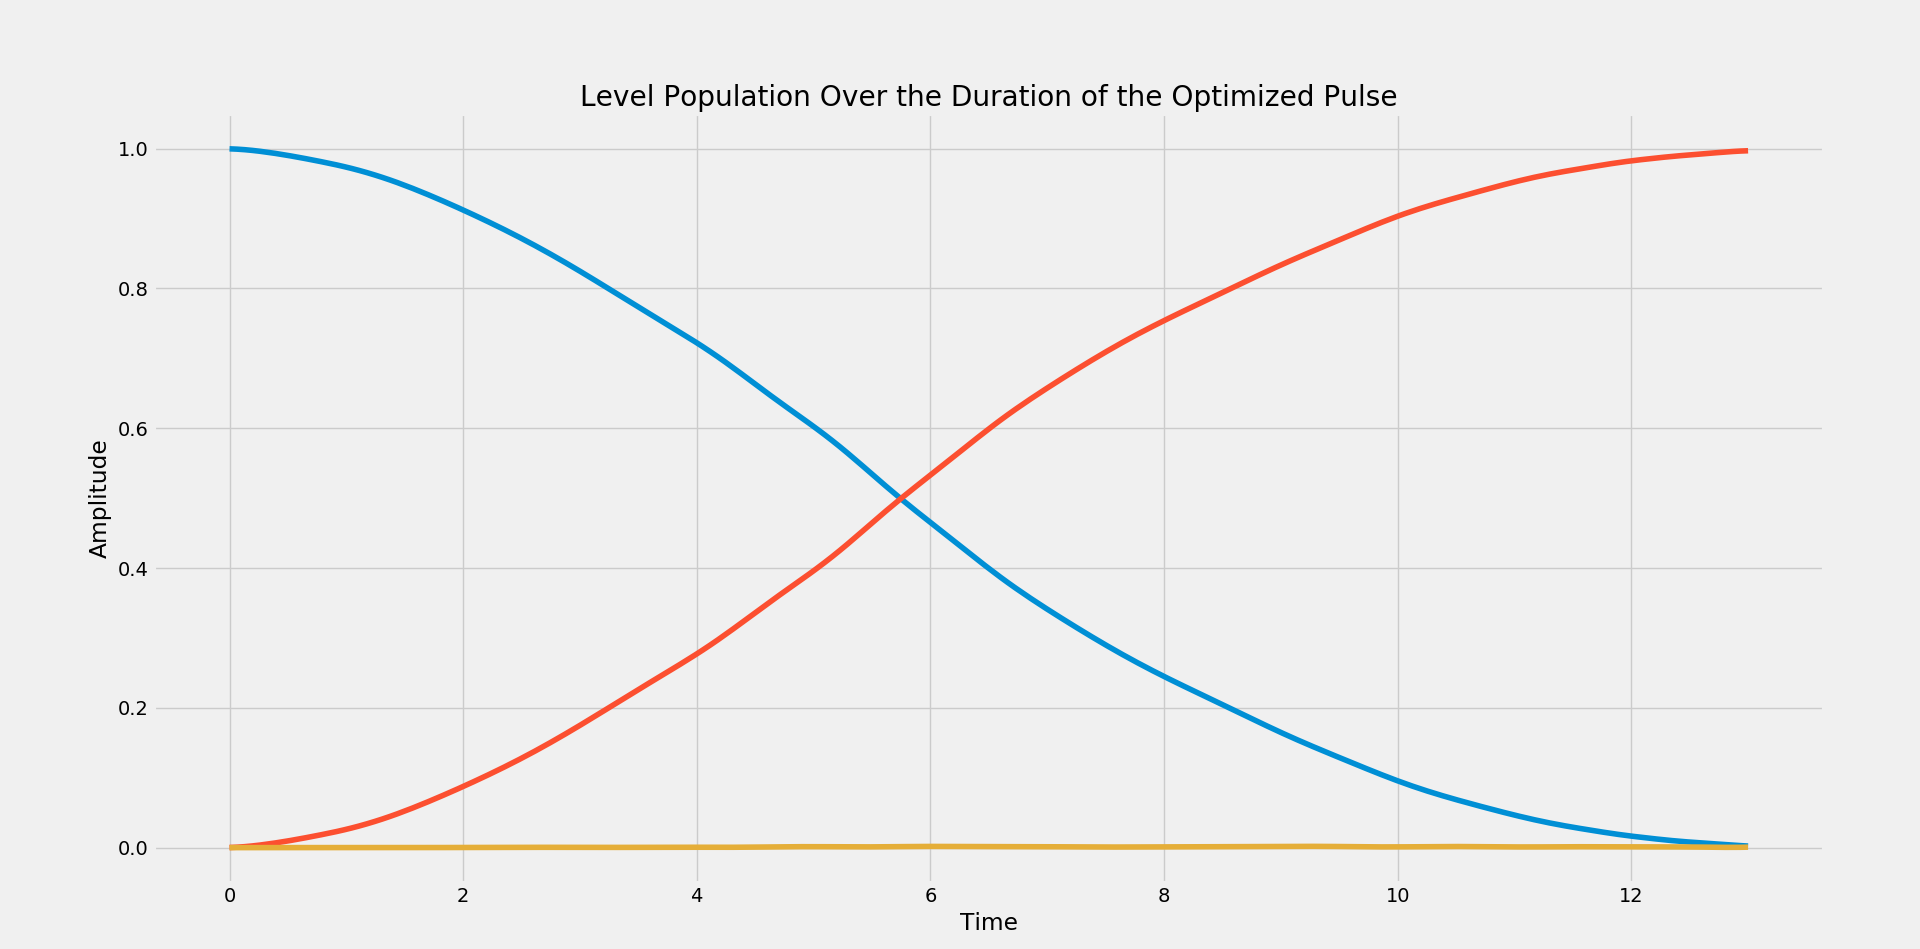
\includegraphics[width=1\columnwidth]{Results/DRAG/level-population2.png}
%     \caption{Level population of the "qubit" over the duration of the pulse that was found by the GRAPE algorithm, with all the penalties turned on, including the DRAG penalty.}
%     \label{fig:sDRAG-results}
% \end{figure}
\begin{figure}[H]
    \begin{center}
        %% Creator: Matplotlib, PGF backend
%%
%% To include the figure in your LaTeX document, write
%%   \input{<filename>.pgf}
%%
%% Make sure the required packages are loaded in your preamble
%%   \usepackage{pgf}
%%
%% and, on pdftex
%%   \usepackage[utf8]{inputenc}\DeclareUnicodeCharacter{2212}{-}
%%
%% or, on luatex and xetex
%%   \usepackage{unicode-math}
%%
%% Figures using additional raster images can only be included by \input if
%% they are in the same directory as the main LaTeX file. For loading figures
%% from other directories you can use the `import` package
%%   \usepackage{import}
%%
%% and then include the figures with
%%   \import{<path to file>}{<filename>.pgf}
%%
%% Matplotlib used the following preamble
%%
\begingroup%
\makeatletter%
\begin{pgfpicture}%
\pgfpathrectangle{\pgfpointorigin}{\pgfqpoint{4.650000in}{2.300000in}}%
\pgfusepath{use as bounding box, clip}%
\begin{pgfscope}%
\pgfsetbuttcap%
\pgfsetmiterjoin%
\definecolor{currentfill}{rgb}{1.000000,1.000000,1.000000}%
\pgfsetfillcolor{currentfill}%
\pgfsetlinewidth{0.000000pt}%
\definecolor{currentstroke}{rgb}{1.000000,1.000000,1.000000}%
\pgfsetstrokecolor{currentstroke}%
\pgfsetdash{}{0pt}%
\pgfpathmoveto{\pgfqpoint{0.000000in}{0.000000in}}%
\pgfpathlineto{\pgfqpoint{4.650000in}{0.000000in}}%
\pgfpathlineto{\pgfqpoint{4.650000in}{2.300000in}}%
\pgfpathlineto{\pgfqpoint{0.000000in}{2.300000in}}%
\pgfpathclose%
\pgfusepath{fill}%
\end{pgfscope}%
\begin{pgfscope}%
\pgfsetbuttcap%
\pgfsetmiterjoin%
\definecolor{currentfill}{rgb}{1.000000,1.000000,1.000000}%
\pgfsetfillcolor{currentfill}%
\pgfsetlinewidth{0.000000pt}%
\definecolor{currentstroke}{rgb}{0.000000,0.000000,0.000000}%
\pgfsetstrokecolor{currentstroke}%
\pgfsetstrokeopacity{0.000000}%
\pgfsetdash{}{0pt}%
\pgfpathmoveto{\pgfqpoint{0.646914in}{0.370679in}}%
\pgfpathlineto{\pgfqpoint{2.474152in}{0.370679in}}%
\pgfpathlineto{\pgfqpoint{2.474152in}{1.927778in}}%
\pgfpathlineto{\pgfqpoint{0.646914in}{1.927778in}}%
\pgfpathclose%
\pgfusepath{fill}%
\end{pgfscope}%
\begin{pgfscope}%
\pgfpathrectangle{\pgfqpoint{0.646914in}{0.370679in}}{\pgfqpoint{1.827237in}{1.557099in}}%
\pgfusepath{clip}%
\pgfsetrectcap%
\pgfsetroundjoin%
\pgfsetlinewidth{0.803000pt}%
\definecolor{currentstroke}{rgb}{0.501961,0.501961,0.501961}%
\pgfsetstrokecolor{currentstroke}%
\pgfsetstrokeopacity{0.200000}%
\pgfsetdash{}{0pt}%
\pgfpathmoveto{\pgfqpoint{0.729970in}{0.370679in}}%
\pgfpathlineto{\pgfqpoint{0.729970in}{1.927778in}}%
\pgfusepath{stroke}%
\end{pgfscope}%
\begin{pgfscope}%
\pgfsetbuttcap%
\pgfsetroundjoin%
\definecolor{currentfill}{rgb}{0.333333,0.333333,0.333333}%
\pgfsetfillcolor{currentfill}%
\pgfsetlinewidth{0.803000pt}%
\definecolor{currentstroke}{rgb}{0.333333,0.333333,0.333333}%
\pgfsetstrokecolor{currentstroke}%
\pgfsetdash{}{0pt}%
\pgfsys@defobject{currentmarker}{\pgfqpoint{0.000000in}{-0.048611in}}{\pgfqpoint{0.000000in}{0.000000in}}{%
\pgfpathmoveto{\pgfqpoint{0.000000in}{0.000000in}}%
\pgfpathlineto{\pgfqpoint{0.000000in}{-0.048611in}}%
\pgfusepath{stroke,fill}%
}%
\begin{pgfscope}%
\pgfsys@transformshift{0.729970in}{0.370679in}%
\pgfsys@useobject{currentmarker}{}%
\end{pgfscope}%
\end{pgfscope}%
\begin{pgfscope}%
\definecolor{textcolor}{rgb}{0.333333,0.333333,0.333333}%
\pgfsetstrokecolor{textcolor}%
\pgfsetfillcolor{textcolor}%
\pgftext[x=0.729970in,y=0.273457in,,top]{\color{textcolor}\rmfamily\fontsize{10.000000}{12.000000}\selectfont \(\displaystyle {0}\)}%
\end{pgfscope}%
\begin{pgfscope}%
\pgfpathrectangle{\pgfqpoint{0.646914in}{0.370679in}}{\pgfqpoint{1.827237in}{1.557099in}}%
\pgfusepath{clip}%
\pgfsetrectcap%
\pgfsetroundjoin%
\pgfsetlinewidth{0.803000pt}%
\definecolor{currentstroke}{rgb}{0.501961,0.501961,0.501961}%
\pgfsetstrokecolor{currentstroke}%
\pgfsetstrokeopacity{0.200000}%
\pgfsetdash{}{0pt}%
\pgfpathmoveto{\pgfqpoint{1.394420in}{0.370679in}}%
\pgfpathlineto{\pgfqpoint{1.394420in}{1.927778in}}%
\pgfusepath{stroke}%
\end{pgfscope}%
\begin{pgfscope}%
\pgfsetbuttcap%
\pgfsetroundjoin%
\definecolor{currentfill}{rgb}{0.333333,0.333333,0.333333}%
\pgfsetfillcolor{currentfill}%
\pgfsetlinewidth{0.803000pt}%
\definecolor{currentstroke}{rgb}{0.333333,0.333333,0.333333}%
\pgfsetstrokecolor{currentstroke}%
\pgfsetdash{}{0pt}%
\pgfsys@defobject{currentmarker}{\pgfqpoint{0.000000in}{-0.048611in}}{\pgfqpoint{0.000000in}{0.000000in}}{%
\pgfpathmoveto{\pgfqpoint{0.000000in}{0.000000in}}%
\pgfpathlineto{\pgfqpoint{0.000000in}{-0.048611in}}%
\pgfusepath{stroke,fill}%
}%
\begin{pgfscope}%
\pgfsys@transformshift{1.394420in}{0.370679in}%
\pgfsys@useobject{currentmarker}{}%
\end{pgfscope}%
\end{pgfscope}%
\begin{pgfscope}%
\definecolor{textcolor}{rgb}{0.333333,0.333333,0.333333}%
\pgfsetstrokecolor{textcolor}%
\pgfsetfillcolor{textcolor}%
\pgftext[x=1.394420in,y=0.273457in,,top]{\color{textcolor}\rmfamily\fontsize{10.000000}{12.000000}\selectfont \(\displaystyle {10}\)}%
\end{pgfscope}%
\begin{pgfscope}%
\pgfpathrectangle{\pgfqpoint{0.646914in}{0.370679in}}{\pgfqpoint{1.827237in}{1.557099in}}%
\pgfusepath{clip}%
\pgfsetrectcap%
\pgfsetroundjoin%
\pgfsetlinewidth{0.803000pt}%
\definecolor{currentstroke}{rgb}{0.501961,0.501961,0.501961}%
\pgfsetstrokecolor{currentstroke}%
\pgfsetstrokeopacity{0.200000}%
\pgfsetdash{}{0pt}%
\pgfpathmoveto{\pgfqpoint{2.058870in}{0.370679in}}%
\pgfpathlineto{\pgfqpoint{2.058870in}{1.927778in}}%
\pgfusepath{stroke}%
\end{pgfscope}%
\begin{pgfscope}%
\pgfsetbuttcap%
\pgfsetroundjoin%
\definecolor{currentfill}{rgb}{0.333333,0.333333,0.333333}%
\pgfsetfillcolor{currentfill}%
\pgfsetlinewidth{0.803000pt}%
\definecolor{currentstroke}{rgb}{0.333333,0.333333,0.333333}%
\pgfsetstrokecolor{currentstroke}%
\pgfsetdash{}{0pt}%
\pgfsys@defobject{currentmarker}{\pgfqpoint{0.000000in}{-0.048611in}}{\pgfqpoint{0.000000in}{0.000000in}}{%
\pgfpathmoveto{\pgfqpoint{0.000000in}{0.000000in}}%
\pgfpathlineto{\pgfqpoint{0.000000in}{-0.048611in}}%
\pgfusepath{stroke,fill}%
}%
\begin{pgfscope}%
\pgfsys@transformshift{2.058870in}{0.370679in}%
\pgfsys@useobject{currentmarker}{}%
\end{pgfscope}%
\end{pgfscope}%
\begin{pgfscope}%
\definecolor{textcolor}{rgb}{0.333333,0.333333,0.333333}%
\pgfsetstrokecolor{textcolor}%
\pgfsetfillcolor{textcolor}%
\pgftext[x=2.058870in,y=0.273457in,,top]{\color{textcolor}\rmfamily\fontsize{10.000000}{12.000000}\selectfont \(\displaystyle {20}\)}%
\end{pgfscope}%
\begin{pgfscope}%
\pgfpathrectangle{\pgfqpoint{0.646914in}{0.370679in}}{\pgfqpoint{1.827237in}{1.557099in}}%
\pgfusepath{clip}%
\pgfsetrectcap%
\pgfsetroundjoin%
\pgfsetlinewidth{0.803000pt}%
\definecolor{currentstroke}{rgb}{0.501961,0.501961,0.501961}%
\pgfsetstrokecolor{currentstroke}%
\pgfsetstrokeopacity{0.200000}%
\pgfsetdash{}{0pt}%
\pgfpathmoveto{\pgfqpoint{0.646914in}{0.441456in}}%
\pgfpathlineto{\pgfqpoint{2.474152in}{0.441456in}}%
\pgfusepath{stroke}%
\end{pgfscope}%
\begin{pgfscope}%
\pgfsetbuttcap%
\pgfsetroundjoin%
\definecolor{currentfill}{rgb}{0.333333,0.333333,0.333333}%
\pgfsetfillcolor{currentfill}%
\pgfsetlinewidth{0.803000pt}%
\definecolor{currentstroke}{rgb}{0.333333,0.333333,0.333333}%
\pgfsetstrokecolor{currentstroke}%
\pgfsetdash{}{0pt}%
\pgfsys@defobject{currentmarker}{\pgfqpoint{-0.048611in}{0.000000in}}{\pgfqpoint{0.000000in}{0.000000in}}{%
\pgfpathmoveto{\pgfqpoint{0.000000in}{0.000000in}}%
\pgfpathlineto{\pgfqpoint{-0.048611in}{0.000000in}}%
\pgfusepath{stroke,fill}%
}%
\begin{pgfscope}%
\pgfsys@transformshift{0.646914in}{0.441456in}%
\pgfsys@useobject{currentmarker}{}%
\end{pgfscope}%
\end{pgfscope}%
\begin{pgfscope}%
\definecolor{textcolor}{rgb}{0.333333,0.333333,0.333333}%
\pgfsetstrokecolor{textcolor}%
\pgfsetfillcolor{textcolor}%
\pgftext[x=0.302778in, y=0.393231in, left, base]{\color{textcolor}\rmfamily\fontsize{10.000000}{12.000000}\selectfont \(\displaystyle {0.00}\)}%
\end{pgfscope}%
\begin{pgfscope}%
\pgfpathrectangle{\pgfqpoint{0.646914in}{0.370679in}}{\pgfqpoint{1.827237in}{1.557099in}}%
\pgfusepath{clip}%
\pgfsetrectcap%
\pgfsetroundjoin%
\pgfsetlinewidth{0.803000pt}%
\definecolor{currentstroke}{rgb}{0.501961,0.501961,0.501961}%
\pgfsetstrokecolor{currentstroke}%
\pgfsetstrokeopacity{0.200000}%
\pgfsetdash{}{0pt}%
\pgfpathmoveto{\pgfqpoint{0.646914in}{0.795342in}}%
\pgfpathlineto{\pgfqpoint{2.474152in}{0.795342in}}%
\pgfusepath{stroke}%
\end{pgfscope}%
\begin{pgfscope}%
\pgfsetbuttcap%
\pgfsetroundjoin%
\definecolor{currentfill}{rgb}{0.333333,0.333333,0.333333}%
\pgfsetfillcolor{currentfill}%
\pgfsetlinewidth{0.803000pt}%
\definecolor{currentstroke}{rgb}{0.333333,0.333333,0.333333}%
\pgfsetstrokecolor{currentstroke}%
\pgfsetdash{}{0pt}%
\pgfsys@defobject{currentmarker}{\pgfqpoint{-0.048611in}{0.000000in}}{\pgfqpoint{0.000000in}{0.000000in}}{%
\pgfpathmoveto{\pgfqpoint{0.000000in}{0.000000in}}%
\pgfpathlineto{\pgfqpoint{-0.048611in}{0.000000in}}%
\pgfusepath{stroke,fill}%
}%
\begin{pgfscope}%
\pgfsys@transformshift{0.646914in}{0.795342in}%
\pgfsys@useobject{currentmarker}{}%
\end{pgfscope}%
\end{pgfscope}%
\begin{pgfscope}%
\definecolor{textcolor}{rgb}{0.333333,0.333333,0.333333}%
\pgfsetstrokecolor{textcolor}%
\pgfsetfillcolor{textcolor}%
\pgftext[x=0.302778in, y=0.747117in, left, base]{\color{textcolor}\rmfamily\fontsize{10.000000}{12.000000}\selectfont \(\displaystyle {0.25}\)}%
\end{pgfscope}%
\begin{pgfscope}%
\pgfpathrectangle{\pgfqpoint{0.646914in}{0.370679in}}{\pgfqpoint{1.827237in}{1.557099in}}%
\pgfusepath{clip}%
\pgfsetrectcap%
\pgfsetroundjoin%
\pgfsetlinewidth{0.803000pt}%
\definecolor{currentstroke}{rgb}{0.501961,0.501961,0.501961}%
\pgfsetstrokecolor{currentstroke}%
\pgfsetstrokeopacity{0.200000}%
\pgfsetdash{}{0pt}%
\pgfpathmoveto{\pgfqpoint{0.646914in}{1.149228in}}%
\pgfpathlineto{\pgfqpoint{2.474152in}{1.149228in}}%
\pgfusepath{stroke}%
\end{pgfscope}%
\begin{pgfscope}%
\pgfsetbuttcap%
\pgfsetroundjoin%
\definecolor{currentfill}{rgb}{0.333333,0.333333,0.333333}%
\pgfsetfillcolor{currentfill}%
\pgfsetlinewidth{0.803000pt}%
\definecolor{currentstroke}{rgb}{0.333333,0.333333,0.333333}%
\pgfsetstrokecolor{currentstroke}%
\pgfsetdash{}{0pt}%
\pgfsys@defobject{currentmarker}{\pgfqpoint{-0.048611in}{0.000000in}}{\pgfqpoint{0.000000in}{0.000000in}}{%
\pgfpathmoveto{\pgfqpoint{0.000000in}{0.000000in}}%
\pgfpathlineto{\pgfqpoint{-0.048611in}{0.000000in}}%
\pgfusepath{stroke,fill}%
}%
\begin{pgfscope}%
\pgfsys@transformshift{0.646914in}{1.149228in}%
\pgfsys@useobject{currentmarker}{}%
\end{pgfscope}%
\end{pgfscope}%
\begin{pgfscope}%
\definecolor{textcolor}{rgb}{0.333333,0.333333,0.333333}%
\pgfsetstrokecolor{textcolor}%
\pgfsetfillcolor{textcolor}%
\pgftext[x=0.302778in, y=1.101003in, left, base]{\color{textcolor}\rmfamily\fontsize{10.000000}{12.000000}\selectfont \(\displaystyle {0.50}\)}%
\end{pgfscope}%
\begin{pgfscope}%
\pgfpathrectangle{\pgfqpoint{0.646914in}{0.370679in}}{\pgfqpoint{1.827237in}{1.557099in}}%
\pgfusepath{clip}%
\pgfsetrectcap%
\pgfsetroundjoin%
\pgfsetlinewidth{0.803000pt}%
\definecolor{currentstroke}{rgb}{0.501961,0.501961,0.501961}%
\pgfsetstrokecolor{currentstroke}%
\pgfsetstrokeopacity{0.200000}%
\pgfsetdash{}{0pt}%
\pgfpathmoveto{\pgfqpoint{0.646914in}{1.503115in}}%
\pgfpathlineto{\pgfqpoint{2.474152in}{1.503115in}}%
\pgfusepath{stroke}%
\end{pgfscope}%
\begin{pgfscope}%
\pgfsetbuttcap%
\pgfsetroundjoin%
\definecolor{currentfill}{rgb}{0.333333,0.333333,0.333333}%
\pgfsetfillcolor{currentfill}%
\pgfsetlinewidth{0.803000pt}%
\definecolor{currentstroke}{rgb}{0.333333,0.333333,0.333333}%
\pgfsetstrokecolor{currentstroke}%
\pgfsetdash{}{0pt}%
\pgfsys@defobject{currentmarker}{\pgfqpoint{-0.048611in}{0.000000in}}{\pgfqpoint{0.000000in}{0.000000in}}{%
\pgfpathmoveto{\pgfqpoint{0.000000in}{0.000000in}}%
\pgfpathlineto{\pgfqpoint{-0.048611in}{0.000000in}}%
\pgfusepath{stroke,fill}%
}%
\begin{pgfscope}%
\pgfsys@transformshift{0.646914in}{1.503115in}%
\pgfsys@useobject{currentmarker}{}%
\end{pgfscope}%
\end{pgfscope}%
\begin{pgfscope}%
\definecolor{textcolor}{rgb}{0.333333,0.333333,0.333333}%
\pgfsetstrokecolor{textcolor}%
\pgfsetfillcolor{textcolor}%
\pgftext[x=0.302778in, y=1.454889in, left, base]{\color{textcolor}\rmfamily\fontsize{10.000000}{12.000000}\selectfont \(\displaystyle {0.75}\)}%
\end{pgfscope}%
\begin{pgfscope}%
\pgfpathrectangle{\pgfqpoint{0.646914in}{0.370679in}}{\pgfqpoint{1.827237in}{1.557099in}}%
\pgfusepath{clip}%
\pgfsetrectcap%
\pgfsetroundjoin%
\pgfsetlinewidth{0.803000pt}%
\definecolor{currentstroke}{rgb}{0.501961,0.501961,0.501961}%
\pgfsetstrokecolor{currentstroke}%
\pgfsetstrokeopacity{0.200000}%
\pgfsetdash{}{0pt}%
\pgfpathmoveto{\pgfqpoint{0.646914in}{1.857001in}}%
\pgfpathlineto{\pgfqpoint{2.474152in}{1.857001in}}%
\pgfusepath{stroke}%
\end{pgfscope}%
\begin{pgfscope}%
\pgfsetbuttcap%
\pgfsetroundjoin%
\definecolor{currentfill}{rgb}{0.333333,0.333333,0.333333}%
\pgfsetfillcolor{currentfill}%
\pgfsetlinewidth{0.803000pt}%
\definecolor{currentstroke}{rgb}{0.333333,0.333333,0.333333}%
\pgfsetstrokecolor{currentstroke}%
\pgfsetdash{}{0pt}%
\pgfsys@defobject{currentmarker}{\pgfqpoint{-0.048611in}{0.000000in}}{\pgfqpoint{0.000000in}{0.000000in}}{%
\pgfpathmoveto{\pgfqpoint{0.000000in}{0.000000in}}%
\pgfpathlineto{\pgfqpoint{-0.048611in}{0.000000in}}%
\pgfusepath{stroke,fill}%
}%
\begin{pgfscope}%
\pgfsys@transformshift{0.646914in}{1.857001in}%
\pgfsys@useobject{currentmarker}{}%
\end{pgfscope}%
\end{pgfscope}%
\begin{pgfscope}%
\definecolor{textcolor}{rgb}{0.333333,0.333333,0.333333}%
\pgfsetstrokecolor{textcolor}%
\pgfsetfillcolor{textcolor}%
\pgftext[x=0.302778in, y=1.808776in, left, base]{\color{textcolor}\rmfamily\fontsize{10.000000}{12.000000}\selectfont \(\displaystyle {1.00}\)}%
\end{pgfscope}%
\begin{pgfscope}%
\definecolor{textcolor}{rgb}{0.333333,0.333333,0.333333}%
\pgfsetstrokecolor{textcolor}%
\pgfsetfillcolor{textcolor}%
\pgftext[x=0.247222in,y=1.149228in,,bottom,rotate=90.000000]{\color{textcolor}\rmfamily\fontsize{12.000000}{14.400000}\selectfont Amplitude (MHz)}%
\end{pgfscope}%
\begin{pgfscope}%
\pgfpathrectangle{\pgfqpoint{0.646914in}{0.370679in}}{\pgfqpoint{1.827237in}{1.557099in}}%
\pgfusepath{clip}%
\pgfsetrectcap%
\pgfsetroundjoin%
\pgfsetlinewidth{1.505625pt}%
\definecolor{currentstroke}{rgb}{0.886275,0.290196,0.200000}%
\pgfsetstrokecolor{currentstroke}%
\pgfsetdash{}{0pt}%
\pgfpathmoveto{\pgfqpoint{0.729970in}{1.857001in}}%
\pgfpathlineto{\pgfqpoint{2.391095in}{1.856987in}}%
\pgfpathlineto{\pgfqpoint{2.391095in}{1.856987in}}%
\pgfusepath{stroke}%
\end{pgfscope}%
\begin{pgfscope}%
\pgfpathrectangle{\pgfqpoint{0.646914in}{0.370679in}}{\pgfqpoint{1.827237in}{1.557099in}}%
\pgfusepath{clip}%
\pgfsetrectcap%
\pgfsetroundjoin%
\pgfsetlinewidth{1.505625pt}%
\definecolor{currentstroke}{rgb}{0.203922,0.541176,0.741176}%
\pgfsetstrokecolor{currentstroke}%
\pgfsetdash{}{0pt}%
\pgfpathmoveto{\pgfqpoint{0.729970in}{0.441456in}}%
\pgfpathlineto{\pgfqpoint{2.391095in}{0.441469in}}%
\pgfpathlineto{\pgfqpoint{2.391095in}{0.441469in}}%
\pgfusepath{stroke}%
\end{pgfscope}%
\begin{pgfscope}%
\pgfsetrectcap%
\pgfsetmiterjoin%
\pgfsetlinewidth{1.003750pt}%
\definecolor{currentstroke}{rgb}{1.000000,1.000000,1.000000}%
\pgfsetstrokecolor{currentstroke}%
\pgfsetdash{}{0pt}%
\pgfpathmoveto{\pgfqpoint{0.646914in}{0.370679in}}%
\pgfpathlineto{\pgfqpoint{0.646914in}{1.927778in}}%
\pgfusepath{stroke}%
\end{pgfscope}%
\begin{pgfscope}%
\pgfsetrectcap%
\pgfsetmiterjoin%
\pgfsetlinewidth{1.003750pt}%
\definecolor{currentstroke}{rgb}{1.000000,1.000000,1.000000}%
\pgfsetstrokecolor{currentstroke}%
\pgfsetdash{}{0pt}%
\pgfpathmoveto{\pgfqpoint{2.474152in}{0.370679in}}%
\pgfpathlineto{\pgfqpoint{2.474152in}{1.927778in}}%
\pgfusepath{stroke}%
\end{pgfscope}%
\begin{pgfscope}%
\pgfsetrectcap%
\pgfsetmiterjoin%
\pgfsetlinewidth{1.003750pt}%
\definecolor{currentstroke}{rgb}{1.000000,1.000000,1.000000}%
\pgfsetstrokecolor{currentstroke}%
\pgfsetdash{}{0pt}%
\pgfpathmoveto{\pgfqpoint{0.646914in}{0.370679in}}%
\pgfpathlineto{\pgfqpoint{2.474152in}{0.370679in}}%
\pgfusepath{stroke}%
\end{pgfscope}%
\begin{pgfscope}%
\pgfsetrectcap%
\pgfsetmiterjoin%
\pgfsetlinewidth{1.003750pt}%
\definecolor{currentstroke}{rgb}{1.000000,1.000000,1.000000}%
\pgfsetstrokecolor{currentstroke}%
\pgfsetdash{}{0pt}%
\pgfpathmoveto{\pgfqpoint{0.646914in}{1.927778in}}%
\pgfpathlineto{\pgfqpoint{2.474152in}{1.927778in}}%
\pgfusepath{stroke}%
\end{pgfscope}%
\begin{pgfscope}%
\definecolor{textcolor}{rgb}{0.000000,0.000000,0.000000}%
\pgfsetstrokecolor{textcolor}%
\pgfsetfillcolor{textcolor}%
\pgftext[x=1.560533in,y=2.011111in,,base]{\color{textcolor}\rmfamily\fontsize{14.400000}{17.280000}\selectfont Initial pulse}%
\end{pgfscope}%
\begin{pgfscope}%
\pgfsetbuttcap%
\pgfsetmiterjoin%
\definecolor{currentfill}{rgb}{1.000000,1.000000,1.000000}%
\pgfsetfillcolor{currentfill}%
\pgfsetfillopacity{0.800000}%
\pgfsetlinewidth{0.501875pt}%
\definecolor{currentstroke}{rgb}{0.800000,0.800000,0.800000}%
\pgfsetstrokecolor{currentstroke}%
\pgfsetstrokeopacity{0.800000}%
\pgfsetdash{}{0pt}%
\pgfpathmoveto{\pgfqpoint{1.552179in}{0.920062in}}%
\pgfpathlineto{\pgfqpoint{2.376929in}{0.920062in}}%
\pgfpathquadraticcurveto{\pgfqpoint{2.404707in}{0.920062in}}{\pgfqpoint{2.404707in}{0.947840in}}%
\pgfpathlineto{\pgfqpoint{2.404707in}{1.350617in}}%
\pgfpathquadraticcurveto{\pgfqpoint{2.404707in}{1.378395in}}{\pgfqpoint{2.376929in}{1.378395in}}%
\pgfpathlineto{\pgfqpoint{1.552179in}{1.378395in}}%
\pgfpathquadraticcurveto{\pgfqpoint{1.524402in}{1.378395in}}{\pgfqpoint{1.524402in}{1.350617in}}%
\pgfpathlineto{\pgfqpoint{1.524402in}{0.947840in}}%
\pgfpathquadraticcurveto{\pgfqpoint{1.524402in}{0.920062in}}{\pgfqpoint{1.552179in}{0.920062in}}%
\pgfpathclose%
\pgfusepath{stroke,fill}%
\end{pgfscope}%
\begin{pgfscope}%
\pgfsetrectcap%
\pgfsetroundjoin%
\pgfsetlinewidth{1.505625pt}%
\definecolor{currentstroke}{rgb}{0.886275,0.290196,0.200000}%
\pgfsetstrokecolor{currentstroke}%
\pgfsetdash{}{0pt}%
\pgfpathmoveto{\pgfqpoint{1.579957in}{1.267284in}}%
\pgfpathlineto{\pgfqpoint{1.857735in}{1.267284in}}%
\pgfusepath{stroke}%
\end{pgfscope}%
\begin{pgfscope}%
\definecolor{textcolor}{rgb}{0.000000,0.000000,0.000000}%
\pgfsetstrokecolor{textcolor}%
\pgfsetfillcolor{textcolor}%
\pgftext[x=1.968846in,y=1.218673in,left,base]{\color{textcolor}\rmfamily\fontsize{10.000000}{12.000000}\selectfont \(\displaystyle P(|g\rangle)\)}%
\end{pgfscope}%
\begin{pgfscope}%
\pgfsetrectcap%
\pgfsetroundjoin%
\pgfsetlinewidth{1.505625pt}%
\definecolor{currentstroke}{rgb}{0.203922,0.541176,0.741176}%
\pgfsetstrokecolor{currentstroke}%
\pgfsetdash{}{0pt}%
\pgfpathmoveto{\pgfqpoint{1.579957in}{1.058951in}}%
\pgfpathlineto{\pgfqpoint{1.857735in}{1.058951in}}%
\pgfusepath{stroke}%
\end{pgfscope}%
\begin{pgfscope}%
\definecolor{textcolor}{rgb}{0.000000,0.000000,0.000000}%
\pgfsetstrokecolor{textcolor}%
\pgfsetfillcolor{textcolor}%
\pgftext[x=1.968846in,y=1.010340in,left,base]{\color{textcolor}\rmfamily\fontsize{10.000000}{12.000000}\selectfont \(\displaystyle P(|e\rangle)\)}%
\end{pgfscope}%
\begin{pgfscope}%
\pgfsetbuttcap%
\pgfsetmiterjoin%
\definecolor{currentfill}{rgb}{1.000000,1.000000,1.000000}%
\pgfsetfillcolor{currentfill}%
\pgfsetlinewidth{0.000000pt}%
\definecolor{currentstroke}{rgb}{0.000000,0.000000,0.000000}%
\pgfsetstrokecolor{currentstroke}%
\pgfsetstrokeopacity{0.000000}%
\pgfsetdash{}{0pt}%
\pgfpathmoveto{\pgfqpoint{2.672763in}{0.370679in}}%
\pgfpathlineto{\pgfqpoint{4.500000in}{0.370679in}}%
\pgfpathlineto{\pgfqpoint{4.500000in}{1.927778in}}%
\pgfpathlineto{\pgfqpoint{2.672763in}{1.927778in}}%
\pgfpathclose%
\pgfusepath{fill}%
\end{pgfscope}%
\begin{pgfscope}%
\pgfpathrectangle{\pgfqpoint{2.672763in}{0.370679in}}{\pgfqpoint{1.827237in}{1.557099in}}%
\pgfusepath{clip}%
\pgfsetrectcap%
\pgfsetroundjoin%
\pgfsetlinewidth{0.803000pt}%
\definecolor{currentstroke}{rgb}{0.501961,0.501961,0.501961}%
\pgfsetstrokecolor{currentstroke}%
\pgfsetstrokeopacity{0.200000}%
\pgfsetdash{}{0pt}%
\pgfpathmoveto{\pgfqpoint{2.755819in}{0.370679in}}%
\pgfpathlineto{\pgfqpoint{2.755819in}{1.927778in}}%
\pgfusepath{stroke}%
\end{pgfscope}%
\begin{pgfscope}%
\pgfsetbuttcap%
\pgfsetroundjoin%
\definecolor{currentfill}{rgb}{0.333333,0.333333,0.333333}%
\pgfsetfillcolor{currentfill}%
\pgfsetlinewidth{0.803000pt}%
\definecolor{currentstroke}{rgb}{0.333333,0.333333,0.333333}%
\pgfsetstrokecolor{currentstroke}%
\pgfsetdash{}{0pt}%
\pgfsys@defobject{currentmarker}{\pgfqpoint{0.000000in}{-0.048611in}}{\pgfqpoint{0.000000in}{0.000000in}}{%
\pgfpathmoveto{\pgfqpoint{0.000000in}{0.000000in}}%
\pgfpathlineto{\pgfqpoint{0.000000in}{-0.048611in}}%
\pgfusepath{stroke,fill}%
}%
\begin{pgfscope}%
\pgfsys@transformshift{2.755819in}{0.370679in}%
\pgfsys@useobject{currentmarker}{}%
\end{pgfscope}%
\end{pgfscope}%
\begin{pgfscope}%
\definecolor{textcolor}{rgb}{0.333333,0.333333,0.333333}%
\pgfsetstrokecolor{textcolor}%
\pgfsetfillcolor{textcolor}%
\pgftext[x=2.755819in,y=0.273457in,,top]{\color{textcolor}\rmfamily\fontsize{10.000000}{12.000000}\selectfont \(\displaystyle {0}\)}%
\end{pgfscope}%
\begin{pgfscope}%
\pgfpathrectangle{\pgfqpoint{2.672763in}{0.370679in}}{\pgfqpoint{1.827237in}{1.557099in}}%
\pgfusepath{clip}%
\pgfsetrectcap%
\pgfsetroundjoin%
\pgfsetlinewidth{0.803000pt}%
\definecolor{currentstroke}{rgb}{0.501961,0.501961,0.501961}%
\pgfsetstrokecolor{currentstroke}%
\pgfsetstrokeopacity{0.200000}%
\pgfsetdash{}{0pt}%
\pgfpathmoveto{\pgfqpoint{3.420269in}{0.370679in}}%
\pgfpathlineto{\pgfqpoint{3.420269in}{1.927778in}}%
\pgfusepath{stroke}%
\end{pgfscope}%
\begin{pgfscope}%
\pgfsetbuttcap%
\pgfsetroundjoin%
\definecolor{currentfill}{rgb}{0.333333,0.333333,0.333333}%
\pgfsetfillcolor{currentfill}%
\pgfsetlinewidth{0.803000pt}%
\definecolor{currentstroke}{rgb}{0.333333,0.333333,0.333333}%
\pgfsetstrokecolor{currentstroke}%
\pgfsetdash{}{0pt}%
\pgfsys@defobject{currentmarker}{\pgfqpoint{0.000000in}{-0.048611in}}{\pgfqpoint{0.000000in}{0.000000in}}{%
\pgfpathmoveto{\pgfqpoint{0.000000in}{0.000000in}}%
\pgfpathlineto{\pgfqpoint{0.000000in}{-0.048611in}}%
\pgfusepath{stroke,fill}%
}%
\begin{pgfscope}%
\pgfsys@transformshift{3.420269in}{0.370679in}%
\pgfsys@useobject{currentmarker}{}%
\end{pgfscope}%
\end{pgfscope}%
\begin{pgfscope}%
\definecolor{textcolor}{rgb}{0.333333,0.333333,0.333333}%
\pgfsetstrokecolor{textcolor}%
\pgfsetfillcolor{textcolor}%
\pgftext[x=3.420269in,y=0.273457in,,top]{\color{textcolor}\rmfamily\fontsize{10.000000}{12.000000}\selectfont \(\displaystyle {10}\)}%
\end{pgfscope}%
\begin{pgfscope}%
\pgfpathrectangle{\pgfqpoint{2.672763in}{0.370679in}}{\pgfqpoint{1.827237in}{1.557099in}}%
\pgfusepath{clip}%
\pgfsetrectcap%
\pgfsetroundjoin%
\pgfsetlinewidth{0.803000pt}%
\definecolor{currentstroke}{rgb}{0.501961,0.501961,0.501961}%
\pgfsetstrokecolor{currentstroke}%
\pgfsetstrokeopacity{0.200000}%
\pgfsetdash{}{0pt}%
\pgfpathmoveto{\pgfqpoint{4.084719in}{0.370679in}}%
\pgfpathlineto{\pgfqpoint{4.084719in}{1.927778in}}%
\pgfusepath{stroke}%
\end{pgfscope}%
\begin{pgfscope}%
\pgfsetbuttcap%
\pgfsetroundjoin%
\definecolor{currentfill}{rgb}{0.333333,0.333333,0.333333}%
\pgfsetfillcolor{currentfill}%
\pgfsetlinewidth{0.803000pt}%
\definecolor{currentstroke}{rgb}{0.333333,0.333333,0.333333}%
\pgfsetstrokecolor{currentstroke}%
\pgfsetdash{}{0pt}%
\pgfsys@defobject{currentmarker}{\pgfqpoint{0.000000in}{-0.048611in}}{\pgfqpoint{0.000000in}{0.000000in}}{%
\pgfpathmoveto{\pgfqpoint{0.000000in}{0.000000in}}%
\pgfpathlineto{\pgfqpoint{0.000000in}{-0.048611in}}%
\pgfusepath{stroke,fill}%
}%
\begin{pgfscope}%
\pgfsys@transformshift{4.084719in}{0.370679in}%
\pgfsys@useobject{currentmarker}{}%
\end{pgfscope}%
\end{pgfscope}%
\begin{pgfscope}%
\definecolor{textcolor}{rgb}{0.333333,0.333333,0.333333}%
\pgfsetstrokecolor{textcolor}%
\pgfsetfillcolor{textcolor}%
\pgftext[x=4.084719in,y=0.273457in,,top]{\color{textcolor}\rmfamily\fontsize{10.000000}{12.000000}\selectfont \(\displaystyle {20}\)}%
\end{pgfscope}%
\begin{pgfscope}%
\pgfpathrectangle{\pgfqpoint{2.672763in}{0.370679in}}{\pgfqpoint{1.827237in}{1.557099in}}%
\pgfusepath{clip}%
\pgfsetrectcap%
\pgfsetroundjoin%
\pgfsetlinewidth{0.803000pt}%
\definecolor{currentstroke}{rgb}{0.501961,0.501961,0.501961}%
\pgfsetstrokecolor{currentstroke}%
\pgfsetstrokeopacity{0.200000}%
\pgfsetdash{}{0pt}%
\pgfpathmoveto{\pgfqpoint{2.672763in}{0.441456in}}%
\pgfpathlineto{\pgfqpoint{4.500000in}{0.441456in}}%
\pgfusepath{stroke}%
\end{pgfscope}%
\begin{pgfscope}%
\pgfsetbuttcap%
\pgfsetroundjoin%
\definecolor{currentfill}{rgb}{0.333333,0.333333,0.333333}%
\pgfsetfillcolor{currentfill}%
\pgfsetlinewidth{0.803000pt}%
\definecolor{currentstroke}{rgb}{0.333333,0.333333,0.333333}%
\pgfsetstrokecolor{currentstroke}%
\pgfsetdash{}{0pt}%
\pgfsys@defobject{currentmarker}{\pgfqpoint{-0.048611in}{0.000000in}}{\pgfqpoint{0.000000in}{0.000000in}}{%
\pgfpathmoveto{\pgfqpoint{0.000000in}{0.000000in}}%
\pgfpathlineto{\pgfqpoint{-0.048611in}{0.000000in}}%
\pgfusepath{stroke,fill}%
}%
\begin{pgfscope}%
\pgfsys@transformshift{2.672763in}{0.441456in}%
\pgfsys@useobject{currentmarker}{}%
\end{pgfscope}%
\end{pgfscope}%
\begin{pgfscope}%
\pgfpathrectangle{\pgfqpoint{2.672763in}{0.370679in}}{\pgfqpoint{1.827237in}{1.557099in}}%
\pgfusepath{clip}%
\pgfsetrectcap%
\pgfsetroundjoin%
\pgfsetlinewidth{0.803000pt}%
\definecolor{currentstroke}{rgb}{0.501961,0.501961,0.501961}%
\pgfsetstrokecolor{currentstroke}%
\pgfsetstrokeopacity{0.200000}%
\pgfsetdash{}{0pt}%
\pgfpathmoveto{\pgfqpoint{2.672763in}{0.795342in}}%
\pgfpathlineto{\pgfqpoint{4.500000in}{0.795342in}}%
\pgfusepath{stroke}%
\end{pgfscope}%
\begin{pgfscope}%
\pgfsetbuttcap%
\pgfsetroundjoin%
\definecolor{currentfill}{rgb}{0.333333,0.333333,0.333333}%
\pgfsetfillcolor{currentfill}%
\pgfsetlinewidth{0.803000pt}%
\definecolor{currentstroke}{rgb}{0.333333,0.333333,0.333333}%
\pgfsetstrokecolor{currentstroke}%
\pgfsetdash{}{0pt}%
\pgfsys@defobject{currentmarker}{\pgfqpoint{-0.048611in}{0.000000in}}{\pgfqpoint{0.000000in}{0.000000in}}{%
\pgfpathmoveto{\pgfqpoint{0.000000in}{0.000000in}}%
\pgfpathlineto{\pgfqpoint{-0.048611in}{0.000000in}}%
\pgfusepath{stroke,fill}%
}%
\begin{pgfscope}%
\pgfsys@transformshift{2.672763in}{0.795342in}%
\pgfsys@useobject{currentmarker}{}%
\end{pgfscope}%
\end{pgfscope}%
\begin{pgfscope}%
\pgfpathrectangle{\pgfqpoint{2.672763in}{0.370679in}}{\pgfqpoint{1.827237in}{1.557099in}}%
\pgfusepath{clip}%
\pgfsetrectcap%
\pgfsetroundjoin%
\pgfsetlinewidth{0.803000pt}%
\definecolor{currentstroke}{rgb}{0.501961,0.501961,0.501961}%
\pgfsetstrokecolor{currentstroke}%
\pgfsetstrokeopacity{0.200000}%
\pgfsetdash{}{0pt}%
\pgfpathmoveto{\pgfqpoint{2.672763in}{1.149228in}}%
\pgfpathlineto{\pgfqpoint{4.500000in}{1.149228in}}%
\pgfusepath{stroke}%
\end{pgfscope}%
\begin{pgfscope}%
\pgfsetbuttcap%
\pgfsetroundjoin%
\definecolor{currentfill}{rgb}{0.333333,0.333333,0.333333}%
\pgfsetfillcolor{currentfill}%
\pgfsetlinewidth{0.803000pt}%
\definecolor{currentstroke}{rgb}{0.333333,0.333333,0.333333}%
\pgfsetstrokecolor{currentstroke}%
\pgfsetdash{}{0pt}%
\pgfsys@defobject{currentmarker}{\pgfqpoint{-0.048611in}{0.000000in}}{\pgfqpoint{0.000000in}{0.000000in}}{%
\pgfpathmoveto{\pgfqpoint{0.000000in}{0.000000in}}%
\pgfpathlineto{\pgfqpoint{-0.048611in}{0.000000in}}%
\pgfusepath{stroke,fill}%
}%
\begin{pgfscope}%
\pgfsys@transformshift{2.672763in}{1.149228in}%
\pgfsys@useobject{currentmarker}{}%
\end{pgfscope}%
\end{pgfscope}%
\begin{pgfscope}%
\pgfpathrectangle{\pgfqpoint{2.672763in}{0.370679in}}{\pgfqpoint{1.827237in}{1.557099in}}%
\pgfusepath{clip}%
\pgfsetrectcap%
\pgfsetroundjoin%
\pgfsetlinewidth{0.803000pt}%
\definecolor{currentstroke}{rgb}{0.501961,0.501961,0.501961}%
\pgfsetstrokecolor{currentstroke}%
\pgfsetstrokeopacity{0.200000}%
\pgfsetdash{}{0pt}%
\pgfpathmoveto{\pgfqpoint{2.672763in}{1.503115in}}%
\pgfpathlineto{\pgfqpoint{4.500000in}{1.503115in}}%
\pgfusepath{stroke}%
\end{pgfscope}%
\begin{pgfscope}%
\pgfsetbuttcap%
\pgfsetroundjoin%
\definecolor{currentfill}{rgb}{0.333333,0.333333,0.333333}%
\pgfsetfillcolor{currentfill}%
\pgfsetlinewidth{0.803000pt}%
\definecolor{currentstroke}{rgb}{0.333333,0.333333,0.333333}%
\pgfsetstrokecolor{currentstroke}%
\pgfsetdash{}{0pt}%
\pgfsys@defobject{currentmarker}{\pgfqpoint{-0.048611in}{0.000000in}}{\pgfqpoint{0.000000in}{0.000000in}}{%
\pgfpathmoveto{\pgfqpoint{0.000000in}{0.000000in}}%
\pgfpathlineto{\pgfqpoint{-0.048611in}{0.000000in}}%
\pgfusepath{stroke,fill}%
}%
\begin{pgfscope}%
\pgfsys@transformshift{2.672763in}{1.503115in}%
\pgfsys@useobject{currentmarker}{}%
\end{pgfscope}%
\end{pgfscope}%
\begin{pgfscope}%
\pgfpathrectangle{\pgfqpoint{2.672763in}{0.370679in}}{\pgfqpoint{1.827237in}{1.557099in}}%
\pgfusepath{clip}%
\pgfsetrectcap%
\pgfsetroundjoin%
\pgfsetlinewidth{0.803000pt}%
\definecolor{currentstroke}{rgb}{0.501961,0.501961,0.501961}%
\pgfsetstrokecolor{currentstroke}%
\pgfsetstrokeopacity{0.200000}%
\pgfsetdash{}{0pt}%
\pgfpathmoveto{\pgfqpoint{2.672763in}{1.857001in}}%
\pgfpathlineto{\pgfqpoint{4.500000in}{1.857001in}}%
\pgfusepath{stroke}%
\end{pgfscope}%
\begin{pgfscope}%
\pgfsetbuttcap%
\pgfsetroundjoin%
\definecolor{currentfill}{rgb}{0.333333,0.333333,0.333333}%
\pgfsetfillcolor{currentfill}%
\pgfsetlinewidth{0.803000pt}%
\definecolor{currentstroke}{rgb}{0.333333,0.333333,0.333333}%
\pgfsetstrokecolor{currentstroke}%
\pgfsetdash{}{0pt}%
\pgfsys@defobject{currentmarker}{\pgfqpoint{-0.048611in}{0.000000in}}{\pgfqpoint{0.000000in}{0.000000in}}{%
\pgfpathmoveto{\pgfqpoint{0.000000in}{0.000000in}}%
\pgfpathlineto{\pgfqpoint{-0.048611in}{0.000000in}}%
\pgfusepath{stroke,fill}%
}%
\begin{pgfscope}%
\pgfsys@transformshift{2.672763in}{1.857001in}%
\pgfsys@useobject{currentmarker}{}%
\end{pgfscope}%
\end{pgfscope}%
\begin{pgfscope}%
\pgfpathrectangle{\pgfqpoint{2.672763in}{0.370679in}}{\pgfqpoint{1.827237in}{1.557099in}}%
\pgfusepath{clip}%
\pgfsetrectcap%
\pgfsetroundjoin%
\pgfsetlinewidth{1.505625pt}%
\definecolor{currentstroke}{rgb}{0.886275,0.290196,0.200000}%
\pgfsetstrokecolor{currentstroke}%
\pgfsetdash{}{0pt}%
\pgfpathmoveto{\pgfqpoint{2.755819in}{1.856915in}}%
\pgfpathlineto{\pgfqpoint{2.789208in}{1.854853in}}%
\pgfpathlineto{\pgfqpoint{2.822598in}{1.849998in}}%
\pgfpathlineto{\pgfqpoint{2.855987in}{1.842205in}}%
\pgfpathlineto{\pgfqpoint{2.889377in}{1.831577in}}%
\pgfpathlineto{\pgfqpoint{2.922766in}{1.818382in}}%
\pgfpathlineto{\pgfqpoint{2.964503in}{1.797995in}}%
\pgfpathlineto{\pgfqpoint{3.006240in}{1.773568in}}%
\pgfpathlineto{\pgfqpoint{3.047977in}{1.745323in}}%
\pgfpathlineto{\pgfqpoint{3.098061in}{1.707292in}}%
\pgfpathlineto{\pgfqpoint{3.148145in}{1.663981in}}%
\pgfpathlineto{\pgfqpoint{3.189882in}{1.624561in}}%
\pgfpathlineto{\pgfqpoint{3.239966in}{1.573058in}}%
\pgfpathlineto{\pgfqpoint{3.298397in}{1.508591in}}%
\pgfpathlineto{\pgfqpoint{3.348482in}{1.449914in}}%
\pgfpathlineto{\pgfqpoint{3.415260in}{1.365946in}}%
\pgfpathlineto{\pgfqpoint{3.565513in}{1.170061in}}%
\pgfpathlineto{\pgfqpoint{3.732460in}{0.950177in}}%
\pgfpathlineto{\pgfqpoint{3.815934in}{0.847804in}}%
\pgfpathlineto{\pgfqpoint{3.891060in}{0.761994in}}%
\pgfpathlineto{\pgfqpoint{3.949492in}{0.699613in}}%
\pgfpathlineto{\pgfqpoint{3.999576in}{0.649561in}}%
\pgfpathlineto{\pgfqpoint{4.049660in}{0.604309in}}%
\pgfpathlineto{\pgfqpoint{4.091397in}{0.570493in}}%
\pgfpathlineto{\pgfqpoint{4.141481in}{0.534391in}}%
\pgfpathlineto{\pgfqpoint{4.183218in}{0.508237in}}%
\pgfpathlineto{\pgfqpoint{4.224954in}{0.486459in}}%
\pgfpathlineto{\pgfqpoint{4.258344in}{0.472265in}}%
\pgfpathlineto{\pgfqpoint{4.300081in}{0.458408in}}%
\pgfpathlineto{\pgfqpoint{4.333470in}{0.450132in}}%
\pgfpathlineto{\pgfqpoint{4.366860in}{0.444555in}}%
\pgfpathlineto{\pgfqpoint{4.400249in}{0.441789in}}%
\pgfpathlineto{\pgfqpoint{4.416944in}{0.441456in}}%
\pgfpathlineto{\pgfqpoint{4.416944in}{0.441456in}}%
\pgfusepath{stroke}%
\end{pgfscope}%
\begin{pgfscope}%
\pgfpathrectangle{\pgfqpoint{2.672763in}{0.370679in}}{\pgfqpoint{1.827237in}{1.557099in}}%
\pgfusepath{clip}%
\pgfsetrectcap%
\pgfsetroundjoin%
\pgfsetlinewidth{1.505625pt}%
\definecolor{currentstroke}{rgb}{0.203922,0.541176,0.741176}%
\pgfsetstrokecolor{currentstroke}%
\pgfsetdash{}{0pt}%
\pgfpathmoveto{\pgfqpoint{2.755819in}{0.441542in}}%
\pgfpathlineto{\pgfqpoint{2.789208in}{0.443604in}}%
\pgfpathlineto{\pgfqpoint{2.822598in}{0.448458in}}%
\pgfpathlineto{\pgfqpoint{2.855987in}{0.456252in}}%
\pgfpathlineto{\pgfqpoint{2.889377in}{0.466880in}}%
\pgfpathlineto{\pgfqpoint{2.922766in}{0.480075in}}%
\pgfpathlineto{\pgfqpoint{2.964503in}{0.500462in}}%
\pgfpathlineto{\pgfqpoint{3.006240in}{0.524888in}}%
\pgfpathlineto{\pgfqpoint{3.047977in}{0.553134in}}%
\pgfpathlineto{\pgfqpoint{3.098061in}{0.591165in}}%
\pgfpathlineto{\pgfqpoint{3.148145in}{0.634476in}}%
\pgfpathlineto{\pgfqpoint{3.189882in}{0.673896in}}%
\pgfpathlineto{\pgfqpoint{3.239966in}{0.725399in}}%
\pgfpathlineto{\pgfqpoint{3.298397in}{0.789866in}}%
\pgfpathlineto{\pgfqpoint{3.348482in}{0.848543in}}%
\pgfpathlineto{\pgfqpoint{3.415260in}{0.932511in}}%
\pgfpathlineto{\pgfqpoint{3.565513in}{1.128396in}}%
\pgfpathlineto{\pgfqpoint{3.732460in}{1.348280in}}%
\pgfpathlineto{\pgfqpoint{3.815934in}{1.450653in}}%
\pgfpathlineto{\pgfqpoint{3.891060in}{1.536463in}}%
\pgfpathlineto{\pgfqpoint{3.949492in}{1.598844in}}%
\pgfpathlineto{\pgfqpoint{3.999576in}{1.648896in}}%
\pgfpathlineto{\pgfqpoint{4.049660in}{1.694148in}}%
\pgfpathlineto{\pgfqpoint{4.091397in}{1.727964in}}%
\pgfpathlineto{\pgfqpoint{4.141481in}{1.764065in}}%
\pgfpathlineto{\pgfqpoint{4.183218in}{1.790220in}}%
\pgfpathlineto{\pgfqpoint{4.224954in}{1.811998in}}%
\pgfpathlineto{\pgfqpoint{4.258344in}{1.826192in}}%
\pgfpathlineto{\pgfqpoint{4.300081in}{1.840049in}}%
\pgfpathlineto{\pgfqpoint{4.333470in}{1.848325in}}%
\pgfpathlineto{\pgfqpoint{4.366860in}{1.853902in}}%
\pgfpathlineto{\pgfqpoint{4.400249in}{1.856668in}}%
\pgfpathlineto{\pgfqpoint{4.416944in}{1.857001in}}%
\pgfpathlineto{\pgfqpoint{4.416944in}{1.857001in}}%
\pgfusepath{stroke}%
\end{pgfscope}%
\begin{pgfscope}%
\pgfsetrectcap%
\pgfsetmiterjoin%
\pgfsetlinewidth{1.003750pt}%
\definecolor{currentstroke}{rgb}{1.000000,1.000000,1.000000}%
\pgfsetstrokecolor{currentstroke}%
\pgfsetdash{}{0pt}%
\pgfpathmoveto{\pgfqpoint{2.672763in}{0.370679in}}%
\pgfpathlineto{\pgfqpoint{2.672763in}{1.927778in}}%
\pgfusepath{stroke}%
\end{pgfscope}%
\begin{pgfscope}%
\pgfsetrectcap%
\pgfsetmiterjoin%
\pgfsetlinewidth{1.003750pt}%
\definecolor{currentstroke}{rgb}{1.000000,1.000000,1.000000}%
\pgfsetstrokecolor{currentstroke}%
\pgfsetdash{}{0pt}%
\pgfpathmoveto{\pgfqpoint{4.500000in}{0.370679in}}%
\pgfpathlineto{\pgfqpoint{4.500000in}{1.927778in}}%
\pgfusepath{stroke}%
\end{pgfscope}%
\begin{pgfscope}%
\pgfsetrectcap%
\pgfsetmiterjoin%
\pgfsetlinewidth{1.003750pt}%
\definecolor{currentstroke}{rgb}{1.000000,1.000000,1.000000}%
\pgfsetstrokecolor{currentstroke}%
\pgfsetdash{}{0pt}%
\pgfpathmoveto{\pgfqpoint{2.672763in}{0.370679in}}%
\pgfpathlineto{\pgfqpoint{4.500000in}{0.370679in}}%
\pgfusepath{stroke}%
\end{pgfscope}%
\begin{pgfscope}%
\pgfsetrectcap%
\pgfsetmiterjoin%
\pgfsetlinewidth{1.003750pt}%
\definecolor{currentstroke}{rgb}{1.000000,1.000000,1.000000}%
\pgfsetstrokecolor{currentstroke}%
\pgfsetdash{}{0pt}%
\pgfpathmoveto{\pgfqpoint{2.672763in}{1.927778in}}%
\pgfpathlineto{\pgfqpoint{4.500000in}{1.927778in}}%
\pgfusepath{stroke}%
\end{pgfscope}%
\begin{pgfscope}%
\definecolor{textcolor}{rgb}{0.000000,0.000000,0.000000}%
\pgfsetstrokecolor{textcolor}%
\pgfsetfillcolor{textcolor}%
\pgftext[x=3.586381in,y=2.011111in,,base]{\color{textcolor}\rmfamily\fontsize{14.400000}{17.280000}\selectfont Final pulse}%
\end{pgfscope}%
\begin{pgfscope}%
\definecolor{textcolor}{rgb}{0.000000,0.000000,0.000000}%
\pgfsetstrokecolor{textcolor}%
\pgfsetfillcolor{textcolor}%
\pgftext[x=2.325000in,y=0.000000in,,base]{\color{textcolor}\rmfamily\fontsize{12.000000}{14.400000}\selectfont Time (ns)}%
\end{pgfscope}%
\end{pgfpicture}%
\makeatother%
\endgroup%

    \end{center}
    \caption{Level population of the "qubit" over the duration of the pulse that was found by the GRAPE algorithm, with all the penalties turned on, including the DRAG penalty.}
    \label{fig:sDRAG-results}
\end{figure}
Nice! state $\ket{0}$ goes directly to $1$, $\ket{1}$ goes directly to $0$ and the forbidden level is barley changed throughout the pulse (the fidelity gotten from this pulse is around $99.9\%$, so pretty good).

I think that we talked enough about the qubit for now, let's move the the other half of the system, the cavity.

\section{Implementing Cavity Operations}
\subsection{Limiting the photon number} 
\centerline{\say{Hilbert space is a big place.}}
\centerline{- Carlton Caves}
Here's the thing about the cavity levels, there are infinite amount of them. We can make an assumption that the cavity only has $N$ levels, but it is still possible that something happens in the higher levels that may affect the physical result. We want to make sure that everything interesting is contained in the $N$ levels that we have.

This is quite similar to what we did in the previous section with DRAG, we want to put a penalty on the higher levels. Still, there are two main differences. The first, is that there are much more than one or two extra levels, and as we've seen, the method we used in the previous uses very heavy computation and we can't do it for so many levels. The other difference is that we care less about if some higher level is occupied for a part of the pulse. In the cavity there are higher levels and they're all likely to be but \textbf{the reason we're limiting the cavity levels is for computing reasons, not physical ones}. Unlike the cavity, we really want the qubit dynamics to involve only two levels, so it makes sense that we'll use a different penalty to limit the photon number.

The idea is this, we'll define $n_{ph}$ as the highest level we want the cavity to have. Now let's calculate what will happen if the cavity will have another level, for a total of $n_{ph} + 1$. Ideally, nothing will change, the new level should start at 0 probability and end at 0 probability with no change in between. If there is a change, will add a penalty to the pulse, so in the next iteration there will be less of a change. We can do so for any level higher than one, so instead of using only $n_{ph} + 1$ we'll some over $n_{ph} + k$ for reasonable amount of k's.

We'll define $\mathcal{F}_{n_{ph} + k}$ as the fidelity if there were $n_{ph} + k$ levels. Putting the idea into a formula we get that the new cost function is given by
\[
    Cost = \sum_{k=0}^{N} \mathcal{F}_{n_{ph} + k} (\vec{\epsilon}) - \sum_i \lambda_i g_i (\vec{\epsilon})
\]
We can double enforce the penalty if we add a constraint making sure there is no change in the fidelity for different levels
\[
    g_{ph} = \sum_{k_1 \ne k_2} (\mathcal{F}_{n_{ph} + k_1} - \mathcal{F}_{n_{ph} + k_2})^2
\]
The gradient of which is simply the gradient of which is simply
\[
    \frac{\partial g_{ph}}{\partial \epsilon_k} = 2 \sum_{k_1 \ne k_2} [ (\mathcal{F}_{n_{ph} + k_1} - \mathcal{F}_{n_{ph} + k_2}) (\frac{\partial \mathcal{F}_{n_{ph} + k_1}}{\partial \epsilon_k} - \frac{\partial \mathcal{F}_{n_{ph} + k_2}}{\partial \epsilon_k})]
\]
and everything in this expression was previously calculated (they're simply the derivatives of the fidelity and the fidelity itself).

It's important to note that while it might be tempting to leave $n_{ph}$ at a small value so there will be less to calculate (the size of the matrices grows with $n_{ph}^2$), there is good reason to use a high values of $n_{ph}$. Bigger $n_{ph}$ oscillate at higher frequency (since the cavity is simply a harmonic oscillator), so it's possible to use shorter pulses, and since keeping qubit alive is really a major problem, keeping the pulses short is important to be able to accomplish the most with the time we have with the qubit before it dies.
% TODO: Need to go over the last paragraph and check it with Serge to make sure I'm not making anything up

Lets see what happens if we run the transmon-cavity code. We'll only look at the resulting population graph after the optimization. I warn you that the graph is a bit cluttered. You shouldn't look at any specific details or any specific curve, I didn't put a legend explaining what each curve is. We'll look at it then discuss
% \begin{figure}[H]
%     \centering
%     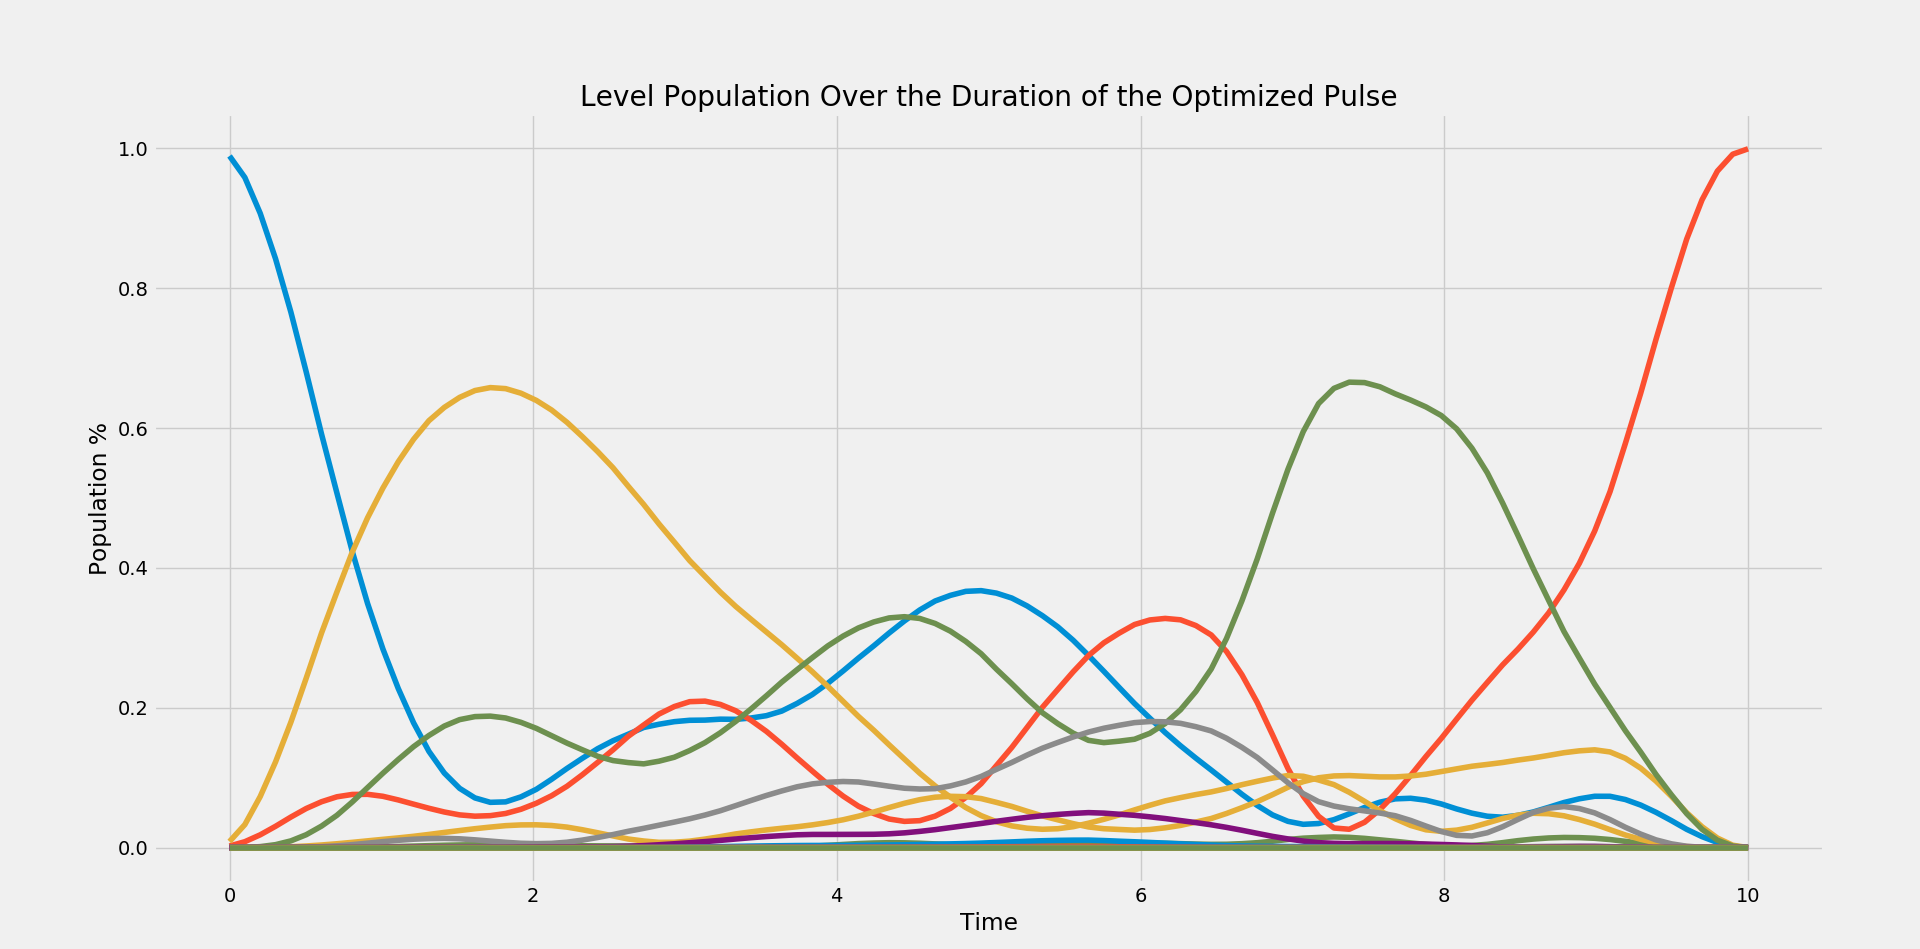
\includegraphics[width=1\columnwidth]{Results/transmon-cavity/g0-g1-level-population.png}
%     \caption{Transmon-cavity state population over the duration of the pulse that does the transformation $\ket{g} \otimes \ket{0}\ \text{ (Blue)} \longrightarrow \ket{g} \otimes \ket{1}\ \text{ (Red)}$.}
%     \label{fig:transmon-cavity-population}
% \end{figure}
\begin{figure}[H]
    \begin{center}
        %% Creator: Matplotlib, PGF backend
%%
%% To include the figure in your LaTeX document, write
%%   \input{<filename>.pgf}
%%
%% Make sure the required packages are loaded in your preamble
%%   \usepackage{pgf}
%%
%% and, on pdftex
%%   \usepackage[utf8]{inputenc}\DeclareUnicodeCharacter{2212}{-}
%%
%% or, on luatex and xetex
%%   \usepackage{unicode-math}
%%
%% Figures using additional raster images can only be included by \input if
%% they are in the same directory as the main LaTeX file. For loading figures
%% from other directories you can use the `import` package
%%   \usepackage{import}
%%
%% and then include the figures with
%%   \import{<path to file>}{<filename>.pgf}
%%
%% Matplotlib used the following preamble
%%
\begingroup%
\makeatletter%
\begin{pgfpicture}%
\pgfpathrectangle{\pgfpointorigin}{\pgfqpoint{4.650000in}{2.300000in}}%
\pgfusepath{use as bounding box, clip}%
\begin{pgfscope}%
\pgfsetbuttcap%
\pgfsetmiterjoin%
\definecolor{currentfill}{rgb}{1.000000,1.000000,1.000000}%
\pgfsetfillcolor{currentfill}%
\pgfsetlinewidth{0.000000pt}%
\definecolor{currentstroke}{rgb}{1.000000,1.000000,1.000000}%
\pgfsetstrokecolor{currentstroke}%
\pgfsetdash{}{0pt}%
\pgfpathmoveto{\pgfqpoint{0.000000in}{0.000000in}}%
\pgfpathlineto{\pgfqpoint{4.650000in}{0.000000in}}%
\pgfpathlineto{\pgfqpoint{4.650000in}{2.300000in}}%
\pgfpathlineto{\pgfqpoint{0.000000in}{2.300000in}}%
\pgfpathclose%
\pgfusepath{fill}%
\end{pgfscope}%
\begin{pgfscope}%
\pgfsetbuttcap%
\pgfsetmiterjoin%
\definecolor{currentfill}{rgb}{1.000000,1.000000,1.000000}%
\pgfsetfillcolor{currentfill}%
\pgfsetlinewidth{0.000000pt}%
\definecolor{currentstroke}{rgb}{0.000000,0.000000,0.000000}%
\pgfsetstrokecolor{currentstroke}%
\pgfsetstrokeopacity{0.000000}%
\pgfsetdash{}{0pt}%
\pgfpathmoveto{\pgfqpoint{0.646914in}{0.370679in}}%
\pgfpathlineto{\pgfqpoint{2.474152in}{0.370679in}}%
\pgfpathlineto{\pgfqpoint{2.474152in}{1.927778in}}%
\pgfpathlineto{\pgfqpoint{0.646914in}{1.927778in}}%
\pgfpathclose%
\pgfusepath{fill}%
\end{pgfscope}%
\begin{pgfscope}%
\pgfpathrectangle{\pgfqpoint{0.646914in}{0.370679in}}{\pgfqpoint{1.827237in}{1.557099in}}%
\pgfusepath{clip}%
\pgfsetrectcap%
\pgfsetroundjoin%
\pgfsetlinewidth{0.803000pt}%
\definecolor{currentstroke}{rgb}{0.501961,0.501961,0.501961}%
\pgfsetstrokecolor{currentstroke}%
\pgfsetstrokeopacity{0.200000}%
\pgfsetdash{}{0pt}%
\pgfpathmoveto{\pgfqpoint{0.729970in}{0.370679in}}%
\pgfpathlineto{\pgfqpoint{0.729970in}{1.927778in}}%
\pgfusepath{stroke}%
\end{pgfscope}%
\begin{pgfscope}%
\pgfsetbuttcap%
\pgfsetroundjoin%
\definecolor{currentfill}{rgb}{0.333333,0.333333,0.333333}%
\pgfsetfillcolor{currentfill}%
\pgfsetlinewidth{0.803000pt}%
\definecolor{currentstroke}{rgb}{0.333333,0.333333,0.333333}%
\pgfsetstrokecolor{currentstroke}%
\pgfsetdash{}{0pt}%
\pgfsys@defobject{currentmarker}{\pgfqpoint{0.000000in}{-0.048611in}}{\pgfqpoint{0.000000in}{0.000000in}}{%
\pgfpathmoveto{\pgfqpoint{0.000000in}{0.000000in}}%
\pgfpathlineto{\pgfqpoint{0.000000in}{-0.048611in}}%
\pgfusepath{stroke,fill}%
}%
\begin{pgfscope}%
\pgfsys@transformshift{0.729970in}{0.370679in}%
\pgfsys@useobject{currentmarker}{}%
\end{pgfscope}%
\end{pgfscope}%
\begin{pgfscope}%
\definecolor{textcolor}{rgb}{0.333333,0.333333,0.333333}%
\pgfsetstrokecolor{textcolor}%
\pgfsetfillcolor{textcolor}%
\pgftext[x=0.729970in,y=0.273457in,,top]{\color{textcolor}\rmfamily\fontsize{10.000000}{12.000000}\selectfont \(\displaystyle {0}\)}%
\end{pgfscope}%
\begin{pgfscope}%
\pgfpathrectangle{\pgfqpoint{0.646914in}{0.370679in}}{\pgfqpoint{1.827237in}{1.557099in}}%
\pgfusepath{clip}%
\pgfsetrectcap%
\pgfsetroundjoin%
\pgfsetlinewidth{0.803000pt}%
\definecolor{currentstroke}{rgb}{0.501961,0.501961,0.501961}%
\pgfsetstrokecolor{currentstroke}%
\pgfsetstrokeopacity{0.200000}%
\pgfsetdash{}{0pt}%
\pgfpathmoveto{\pgfqpoint{1.394420in}{0.370679in}}%
\pgfpathlineto{\pgfqpoint{1.394420in}{1.927778in}}%
\pgfusepath{stroke}%
\end{pgfscope}%
\begin{pgfscope}%
\pgfsetbuttcap%
\pgfsetroundjoin%
\definecolor{currentfill}{rgb}{0.333333,0.333333,0.333333}%
\pgfsetfillcolor{currentfill}%
\pgfsetlinewidth{0.803000pt}%
\definecolor{currentstroke}{rgb}{0.333333,0.333333,0.333333}%
\pgfsetstrokecolor{currentstroke}%
\pgfsetdash{}{0pt}%
\pgfsys@defobject{currentmarker}{\pgfqpoint{0.000000in}{-0.048611in}}{\pgfqpoint{0.000000in}{0.000000in}}{%
\pgfpathmoveto{\pgfqpoint{0.000000in}{0.000000in}}%
\pgfpathlineto{\pgfqpoint{0.000000in}{-0.048611in}}%
\pgfusepath{stroke,fill}%
}%
\begin{pgfscope}%
\pgfsys@transformshift{1.394420in}{0.370679in}%
\pgfsys@useobject{currentmarker}{}%
\end{pgfscope}%
\end{pgfscope}%
\begin{pgfscope}%
\definecolor{textcolor}{rgb}{0.333333,0.333333,0.333333}%
\pgfsetstrokecolor{textcolor}%
\pgfsetfillcolor{textcolor}%
\pgftext[x=1.394420in,y=0.273457in,,top]{\color{textcolor}\rmfamily\fontsize{10.000000}{12.000000}\selectfont \(\displaystyle {10}\)}%
\end{pgfscope}%
\begin{pgfscope}%
\pgfpathrectangle{\pgfqpoint{0.646914in}{0.370679in}}{\pgfqpoint{1.827237in}{1.557099in}}%
\pgfusepath{clip}%
\pgfsetrectcap%
\pgfsetroundjoin%
\pgfsetlinewidth{0.803000pt}%
\definecolor{currentstroke}{rgb}{0.501961,0.501961,0.501961}%
\pgfsetstrokecolor{currentstroke}%
\pgfsetstrokeopacity{0.200000}%
\pgfsetdash{}{0pt}%
\pgfpathmoveto{\pgfqpoint{2.058870in}{0.370679in}}%
\pgfpathlineto{\pgfqpoint{2.058870in}{1.927778in}}%
\pgfusepath{stroke}%
\end{pgfscope}%
\begin{pgfscope}%
\pgfsetbuttcap%
\pgfsetroundjoin%
\definecolor{currentfill}{rgb}{0.333333,0.333333,0.333333}%
\pgfsetfillcolor{currentfill}%
\pgfsetlinewidth{0.803000pt}%
\definecolor{currentstroke}{rgb}{0.333333,0.333333,0.333333}%
\pgfsetstrokecolor{currentstroke}%
\pgfsetdash{}{0pt}%
\pgfsys@defobject{currentmarker}{\pgfqpoint{0.000000in}{-0.048611in}}{\pgfqpoint{0.000000in}{0.000000in}}{%
\pgfpathmoveto{\pgfqpoint{0.000000in}{0.000000in}}%
\pgfpathlineto{\pgfqpoint{0.000000in}{-0.048611in}}%
\pgfusepath{stroke,fill}%
}%
\begin{pgfscope}%
\pgfsys@transformshift{2.058870in}{0.370679in}%
\pgfsys@useobject{currentmarker}{}%
\end{pgfscope}%
\end{pgfscope}%
\begin{pgfscope}%
\definecolor{textcolor}{rgb}{0.333333,0.333333,0.333333}%
\pgfsetstrokecolor{textcolor}%
\pgfsetfillcolor{textcolor}%
\pgftext[x=2.058870in,y=0.273457in,,top]{\color{textcolor}\rmfamily\fontsize{10.000000}{12.000000}\selectfont \(\displaystyle {20}\)}%
\end{pgfscope}%
\begin{pgfscope}%
\pgfpathrectangle{\pgfqpoint{0.646914in}{0.370679in}}{\pgfqpoint{1.827237in}{1.557099in}}%
\pgfusepath{clip}%
\pgfsetrectcap%
\pgfsetroundjoin%
\pgfsetlinewidth{0.803000pt}%
\definecolor{currentstroke}{rgb}{0.501961,0.501961,0.501961}%
\pgfsetstrokecolor{currentstroke}%
\pgfsetstrokeopacity{0.200000}%
\pgfsetdash{}{0pt}%
\pgfpathmoveto{\pgfqpoint{0.646914in}{0.441456in}}%
\pgfpathlineto{\pgfqpoint{2.474152in}{0.441456in}}%
\pgfusepath{stroke}%
\end{pgfscope}%
\begin{pgfscope}%
\pgfsetbuttcap%
\pgfsetroundjoin%
\definecolor{currentfill}{rgb}{0.333333,0.333333,0.333333}%
\pgfsetfillcolor{currentfill}%
\pgfsetlinewidth{0.803000pt}%
\definecolor{currentstroke}{rgb}{0.333333,0.333333,0.333333}%
\pgfsetstrokecolor{currentstroke}%
\pgfsetdash{}{0pt}%
\pgfsys@defobject{currentmarker}{\pgfqpoint{-0.048611in}{0.000000in}}{\pgfqpoint{0.000000in}{0.000000in}}{%
\pgfpathmoveto{\pgfqpoint{0.000000in}{0.000000in}}%
\pgfpathlineto{\pgfqpoint{-0.048611in}{0.000000in}}%
\pgfusepath{stroke,fill}%
}%
\begin{pgfscope}%
\pgfsys@transformshift{0.646914in}{0.441456in}%
\pgfsys@useobject{currentmarker}{}%
\end{pgfscope}%
\end{pgfscope}%
\begin{pgfscope}%
\definecolor{textcolor}{rgb}{0.333333,0.333333,0.333333}%
\pgfsetstrokecolor{textcolor}%
\pgfsetfillcolor{textcolor}%
\pgftext[x=0.302778in, y=0.393231in, left, base]{\color{textcolor}\rmfamily\fontsize{10.000000}{12.000000}\selectfont \(\displaystyle {0.00}\)}%
\end{pgfscope}%
\begin{pgfscope}%
\pgfpathrectangle{\pgfqpoint{0.646914in}{0.370679in}}{\pgfqpoint{1.827237in}{1.557099in}}%
\pgfusepath{clip}%
\pgfsetrectcap%
\pgfsetroundjoin%
\pgfsetlinewidth{0.803000pt}%
\definecolor{currentstroke}{rgb}{0.501961,0.501961,0.501961}%
\pgfsetstrokecolor{currentstroke}%
\pgfsetstrokeopacity{0.200000}%
\pgfsetdash{}{0pt}%
\pgfpathmoveto{\pgfqpoint{0.646914in}{0.795342in}}%
\pgfpathlineto{\pgfqpoint{2.474152in}{0.795342in}}%
\pgfusepath{stroke}%
\end{pgfscope}%
\begin{pgfscope}%
\pgfsetbuttcap%
\pgfsetroundjoin%
\definecolor{currentfill}{rgb}{0.333333,0.333333,0.333333}%
\pgfsetfillcolor{currentfill}%
\pgfsetlinewidth{0.803000pt}%
\definecolor{currentstroke}{rgb}{0.333333,0.333333,0.333333}%
\pgfsetstrokecolor{currentstroke}%
\pgfsetdash{}{0pt}%
\pgfsys@defobject{currentmarker}{\pgfqpoint{-0.048611in}{0.000000in}}{\pgfqpoint{0.000000in}{0.000000in}}{%
\pgfpathmoveto{\pgfqpoint{0.000000in}{0.000000in}}%
\pgfpathlineto{\pgfqpoint{-0.048611in}{0.000000in}}%
\pgfusepath{stroke,fill}%
}%
\begin{pgfscope}%
\pgfsys@transformshift{0.646914in}{0.795342in}%
\pgfsys@useobject{currentmarker}{}%
\end{pgfscope}%
\end{pgfscope}%
\begin{pgfscope}%
\definecolor{textcolor}{rgb}{0.333333,0.333333,0.333333}%
\pgfsetstrokecolor{textcolor}%
\pgfsetfillcolor{textcolor}%
\pgftext[x=0.302778in, y=0.747117in, left, base]{\color{textcolor}\rmfamily\fontsize{10.000000}{12.000000}\selectfont \(\displaystyle {0.25}\)}%
\end{pgfscope}%
\begin{pgfscope}%
\pgfpathrectangle{\pgfqpoint{0.646914in}{0.370679in}}{\pgfqpoint{1.827237in}{1.557099in}}%
\pgfusepath{clip}%
\pgfsetrectcap%
\pgfsetroundjoin%
\pgfsetlinewidth{0.803000pt}%
\definecolor{currentstroke}{rgb}{0.501961,0.501961,0.501961}%
\pgfsetstrokecolor{currentstroke}%
\pgfsetstrokeopacity{0.200000}%
\pgfsetdash{}{0pt}%
\pgfpathmoveto{\pgfqpoint{0.646914in}{1.149228in}}%
\pgfpathlineto{\pgfqpoint{2.474152in}{1.149228in}}%
\pgfusepath{stroke}%
\end{pgfscope}%
\begin{pgfscope}%
\pgfsetbuttcap%
\pgfsetroundjoin%
\definecolor{currentfill}{rgb}{0.333333,0.333333,0.333333}%
\pgfsetfillcolor{currentfill}%
\pgfsetlinewidth{0.803000pt}%
\definecolor{currentstroke}{rgb}{0.333333,0.333333,0.333333}%
\pgfsetstrokecolor{currentstroke}%
\pgfsetdash{}{0pt}%
\pgfsys@defobject{currentmarker}{\pgfqpoint{-0.048611in}{0.000000in}}{\pgfqpoint{0.000000in}{0.000000in}}{%
\pgfpathmoveto{\pgfqpoint{0.000000in}{0.000000in}}%
\pgfpathlineto{\pgfqpoint{-0.048611in}{0.000000in}}%
\pgfusepath{stroke,fill}%
}%
\begin{pgfscope}%
\pgfsys@transformshift{0.646914in}{1.149228in}%
\pgfsys@useobject{currentmarker}{}%
\end{pgfscope}%
\end{pgfscope}%
\begin{pgfscope}%
\definecolor{textcolor}{rgb}{0.333333,0.333333,0.333333}%
\pgfsetstrokecolor{textcolor}%
\pgfsetfillcolor{textcolor}%
\pgftext[x=0.302778in, y=1.101003in, left, base]{\color{textcolor}\rmfamily\fontsize{10.000000}{12.000000}\selectfont \(\displaystyle {0.50}\)}%
\end{pgfscope}%
\begin{pgfscope}%
\pgfpathrectangle{\pgfqpoint{0.646914in}{0.370679in}}{\pgfqpoint{1.827237in}{1.557099in}}%
\pgfusepath{clip}%
\pgfsetrectcap%
\pgfsetroundjoin%
\pgfsetlinewidth{0.803000pt}%
\definecolor{currentstroke}{rgb}{0.501961,0.501961,0.501961}%
\pgfsetstrokecolor{currentstroke}%
\pgfsetstrokeopacity{0.200000}%
\pgfsetdash{}{0pt}%
\pgfpathmoveto{\pgfqpoint{0.646914in}{1.503115in}}%
\pgfpathlineto{\pgfqpoint{2.474152in}{1.503115in}}%
\pgfusepath{stroke}%
\end{pgfscope}%
\begin{pgfscope}%
\pgfsetbuttcap%
\pgfsetroundjoin%
\definecolor{currentfill}{rgb}{0.333333,0.333333,0.333333}%
\pgfsetfillcolor{currentfill}%
\pgfsetlinewidth{0.803000pt}%
\definecolor{currentstroke}{rgb}{0.333333,0.333333,0.333333}%
\pgfsetstrokecolor{currentstroke}%
\pgfsetdash{}{0pt}%
\pgfsys@defobject{currentmarker}{\pgfqpoint{-0.048611in}{0.000000in}}{\pgfqpoint{0.000000in}{0.000000in}}{%
\pgfpathmoveto{\pgfqpoint{0.000000in}{0.000000in}}%
\pgfpathlineto{\pgfqpoint{-0.048611in}{0.000000in}}%
\pgfusepath{stroke,fill}%
}%
\begin{pgfscope}%
\pgfsys@transformshift{0.646914in}{1.503115in}%
\pgfsys@useobject{currentmarker}{}%
\end{pgfscope}%
\end{pgfscope}%
\begin{pgfscope}%
\definecolor{textcolor}{rgb}{0.333333,0.333333,0.333333}%
\pgfsetstrokecolor{textcolor}%
\pgfsetfillcolor{textcolor}%
\pgftext[x=0.302778in, y=1.454889in, left, base]{\color{textcolor}\rmfamily\fontsize{10.000000}{12.000000}\selectfont \(\displaystyle {0.75}\)}%
\end{pgfscope}%
\begin{pgfscope}%
\pgfpathrectangle{\pgfqpoint{0.646914in}{0.370679in}}{\pgfqpoint{1.827237in}{1.557099in}}%
\pgfusepath{clip}%
\pgfsetrectcap%
\pgfsetroundjoin%
\pgfsetlinewidth{0.803000pt}%
\definecolor{currentstroke}{rgb}{0.501961,0.501961,0.501961}%
\pgfsetstrokecolor{currentstroke}%
\pgfsetstrokeopacity{0.200000}%
\pgfsetdash{}{0pt}%
\pgfpathmoveto{\pgfqpoint{0.646914in}{1.857001in}}%
\pgfpathlineto{\pgfqpoint{2.474152in}{1.857001in}}%
\pgfusepath{stroke}%
\end{pgfscope}%
\begin{pgfscope}%
\pgfsetbuttcap%
\pgfsetroundjoin%
\definecolor{currentfill}{rgb}{0.333333,0.333333,0.333333}%
\pgfsetfillcolor{currentfill}%
\pgfsetlinewidth{0.803000pt}%
\definecolor{currentstroke}{rgb}{0.333333,0.333333,0.333333}%
\pgfsetstrokecolor{currentstroke}%
\pgfsetdash{}{0pt}%
\pgfsys@defobject{currentmarker}{\pgfqpoint{-0.048611in}{0.000000in}}{\pgfqpoint{0.000000in}{0.000000in}}{%
\pgfpathmoveto{\pgfqpoint{0.000000in}{0.000000in}}%
\pgfpathlineto{\pgfqpoint{-0.048611in}{0.000000in}}%
\pgfusepath{stroke,fill}%
}%
\begin{pgfscope}%
\pgfsys@transformshift{0.646914in}{1.857001in}%
\pgfsys@useobject{currentmarker}{}%
\end{pgfscope}%
\end{pgfscope}%
\begin{pgfscope}%
\definecolor{textcolor}{rgb}{0.333333,0.333333,0.333333}%
\pgfsetstrokecolor{textcolor}%
\pgfsetfillcolor{textcolor}%
\pgftext[x=0.302778in, y=1.808776in, left, base]{\color{textcolor}\rmfamily\fontsize{10.000000}{12.000000}\selectfont \(\displaystyle {1.00}\)}%
\end{pgfscope}%
\begin{pgfscope}%
\definecolor{textcolor}{rgb}{0.333333,0.333333,0.333333}%
\pgfsetstrokecolor{textcolor}%
\pgfsetfillcolor{textcolor}%
\pgftext[x=0.247222in,y=1.149228in,,bottom,rotate=90.000000]{\color{textcolor}\rmfamily\fontsize{12.000000}{14.400000}\selectfont Amplitude (MHz)}%
\end{pgfscope}%
\begin{pgfscope}%
\pgfpathrectangle{\pgfqpoint{0.646914in}{0.370679in}}{\pgfqpoint{1.827237in}{1.557099in}}%
\pgfusepath{clip}%
\pgfsetrectcap%
\pgfsetroundjoin%
\pgfsetlinewidth{1.505625pt}%
\definecolor{currentstroke}{rgb}{0.886275,0.290196,0.200000}%
\pgfsetstrokecolor{currentstroke}%
\pgfsetdash{}{0pt}%
\pgfpathmoveto{\pgfqpoint{0.729970in}{1.857001in}}%
\pgfpathlineto{\pgfqpoint{2.391095in}{1.856987in}}%
\pgfpathlineto{\pgfqpoint{2.391095in}{1.856987in}}%
\pgfusepath{stroke}%
\end{pgfscope}%
\begin{pgfscope}%
\pgfpathrectangle{\pgfqpoint{0.646914in}{0.370679in}}{\pgfqpoint{1.827237in}{1.557099in}}%
\pgfusepath{clip}%
\pgfsetrectcap%
\pgfsetroundjoin%
\pgfsetlinewidth{1.505625pt}%
\definecolor{currentstroke}{rgb}{0.203922,0.541176,0.741176}%
\pgfsetstrokecolor{currentstroke}%
\pgfsetdash{}{0pt}%
\pgfpathmoveto{\pgfqpoint{0.729970in}{0.441456in}}%
\pgfpathlineto{\pgfqpoint{2.391095in}{0.441469in}}%
\pgfpathlineto{\pgfqpoint{2.391095in}{0.441469in}}%
\pgfusepath{stroke}%
\end{pgfscope}%
\begin{pgfscope}%
\pgfsetrectcap%
\pgfsetmiterjoin%
\pgfsetlinewidth{1.003750pt}%
\definecolor{currentstroke}{rgb}{1.000000,1.000000,1.000000}%
\pgfsetstrokecolor{currentstroke}%
\pgfsetdash{}{0pt}%
\pgfpathmoveto{\pgfqpoint{0.646914in}{0.370679in}}%
\pgfpathlineto{\pgfqpoint{0.646914in}{1.927778in}}%
\pgfusepath{stroke}%
\end{pgfscope}%
\begin{pgfscope}%
\pgfsetrectcap%
\pgfsetmiterjoin%
\pgfsetlinewidth{1.003750pt}%
\definecolor{currentstroke}{rgb}{1.000000,1.000000,1.000000}%
\pgfsetstrokecolor{currentstroke}%
\pgfsetdash{}{0pt}%
\pgfpathmoveto{\pgfqpoint{2.474152in}{0.370679in}}%
\pgfpathlineto{\pgfqpoint{2.474152in}{1.927778in}}%
\pgfusepath{stroke}%
\end{pgfscope}%
\begin{pgfscope}%
\pgfsetrectcap%
\pgfsetmiterjoin%
\pgfsetlinewidth{1.003750pt}%
\definecolor{currentstroke}{rgb}{1.000000,1.000000,1.000000}%
\pgfsetstrokecolor{currentstroke}%
\pgfsetdash{}{0pt}%
\pgfpathmoveto{\pgfqpoint{0.646914in}{0.370679in}}%
\pgfpathlineto{\pgfqpoint{2.474152in}{0.370679in}}%
\pgfusepath{stroke}%
\end{pgfscope}%
\begin{pgfscope}%
\pgfsetrectcap%
\pgfsetmiterjoin%
\pgfsetlinewidth{1.003750pt}%
\definecolor{currentstroke}{rgb}{1.000000,1.000000,1.000000}%
\pgfsetstrokecolor{currentstroke}%
\pgfsetdash{}{0pt}%
\pgfpathmoveto{\pgfqpoint{0.646914in}{1.927778in}}%
\pgfpathlineto{\pgfqpoint{2.474152in}{1.927778in}}%
\pgfusepath{stroke}%
\end{pgfscope}%
\begin{pgfscope}%
\definecolor{textcolor}{rgb}{0.000000,0.000000,0.000000}%
\pgfsetstrokecolor{textcolor}%
\pgfsetfillcolor{textcolor}%
\pgftext[x=1.560533in,y=2.011111in,,base]{\color{textcolor}\rmfamily\fontsize{14.400000}{17.280000}\selectfont Initial pulse}%
\end{pgfscope}%
\begin{pgfscope}%
\pgfsetbuttcap%
\pgfsetmiterjoin%
\definecolor{currentfill}{rgb}{1.000000,1.000000,1.000000}%
\pgfsetfillcolor{currentfill}%
\pgfsetfillopacity{0.800000}%
\pgfsetlinewidth{0.501875pt}%
\definecolor{currentstroke}{rgb}{0.800000,0.800000,0.800000}%
\pgfsetstrokecolor{currentstroke}%
\pgfsetstrokeopacity{0.800000}%
\pgfsetdash{}{0pt}%
\pgfpathmoveto{\pgfqpoint{1.552179in}{0.920062in}}%
\pgfpathlineto{\pgfqpoint{2.376929in}{0.920062in}}%
\pgfpathquadraticcurveto{\pgfqpoint{2.404707in}{0.920062in}}{\pgfqpoint{2.404707in}{0.947840in}}%
\pgfpathlineto{\pgfqpoint{2.404707in}{1.350617in}}%
\pgfpathquadraticcurveto{\pgfqpoint{2.404707in}{1.378395in}}{\pgfqpoint{2.376929in}{1.378395in}}%
\pgfpathlineto{\pgfqpoint{1.552179in}{1.378395in}}%
\pgfpathquadraticcurveto{\pgfqpoint{1.524402in}{1.378395in}}{\pgfqpoint{1.524402in}{1.350617in}}%
\pgfpathlineto{\pgfqpoint{1.524402in}{0.947840in}}%
\pgfpathquadraticcurveto{\pgfqpoint{1.524402in}{0.920062in}}{\pgfqpoint{1.552179in}{0.920062in}}%
\pgfpathclose%
\pgfusepath{stroke,fill}%
\end{pgfscope}%
\begin{pgfscope}%
\pgfsetrectcap%
\pgfsetroundjoin%
\pgfsetlinewidth{1.505625pt}%
\definecolor{currentstroke}{rgb}{0.886275,0.290196,0.200000}%
\pgfsetstrokecolor{currentstroke}%
\pgfsetdash{}{0pt}%
\pgfpathmoveto{\pgfqpoint{1.579957in}{1.267284in}}%
\pgfpathlineto{\pgfqpoint{1.857735in}{1.267284in}}%
\pgfusepath{stroke}%
\end{pgfscope}%
\begin{pgfscope}%
\definecolor{textcolor}{rgb}{0.000000,0.000000,0.000000}%
\pgfsetstrokecolor{textcolor}%
\pgfsetfillcolor{textcolor}%
\pgftext[x=1.968846in,y=1.218673in,left,base]{\color{textcolor}\rmfamily\fontsize{10.000000}{12.000000}\selectfont \(\displaystyle P(|g\rangle)\)}%
\end{pgfscope}%
\begin{pgfscope}%
\pgfsetrectcap%
\pgfsetroundjoin%
\pgfsetlinewidth{1.505625pt}%
\definecolor{currentstroke}{rgb}{0.203922,0.541176,0.741176}%
\pgfsetstrokecolor{currentstroke}%
\pgfsetdash{}{0pt}%
\pgfpathmoveto{\pgfqpoint{1.579957in}{1.058951in}}%
\pgfpathlineto{\pgfqpoint{1.857735in}{1.058951in}}%
\pgfusepath{stroke}%
\end{pgfscope}%
\begin{pgfscope}%
\definecolor{textcolor}{rgb}{0.000000,0.000000,0.000000}%
\pgfsetstrokecolor{textcolor}%
\pgfsetfillcolor{textcolor}%
\pgftext[x=1.968846in,y=1.010340in,left,base]{\color{textcolor}\rmfamily\fontsize{10.000000}{12.000000}\selectfont \(\displaystyle P(|e\rangle)\)}%
\end{pgfscope}%
\begin{pgfscope}%
\pgfsetbuttcap%
\pgfsetmiterjoin%
\definecolor{currentfill}{rgb}{1.000000,1.000000,1.000000}%
\pgfsetfillcolor{currentfill}%
\pgfsetlinewidth{0.000000pt}%
\definecolor{currentstroke}{rgb}{0.000000,0.000000,0.000000}%
\pgfsetstrokecolor{currentstroke}%
\pgfsetstrokeopacity{0.000000}%
\pgfsetdash{}{0pt}%
\pgfpathmoveto{\pgfqpoint{2.672763in}{0.370679in}}%
\pgfpathlineto{\pgfqpoint{4.500000in}{0.370679in}}%
\pgfpathlineto{\pgfqpoint{4.500000in}{1.927778in}}%
\pgfpathlineto{\pgfqpoint{2.672763in}{1.927778in}}%
\pgfpathclose%
\pgfusepath{fill}%
\end{pgfscope}%
\begin{pgfscope}%
\pgfpathrectangle{\pgfqpoint{2.672763in}{0.370679in}}{\pgfqpoint{1.827237in}{1.557099in}}%
\pgfusepath{clip}%
\pgfsetrectcap%
\pgfsetroundjoin%
\pgfsetlinewidth{0.803000pt}%
\definecolor{currentstroke}{rgb}{0.501961,0.501961,0.501961}%
\pgfsetstrokecolor{currentstroke}%
\pgfsetstrokeopacity{0.200000}%
\pgfsetdash{}{0pt}%
\pgfpathmoveto{\pgfqpoint{2.755819in}{0.370679in}}%
\pgfpathlineto{\pgfqpoint{2.755819in}{1.927778in}}%
\pgfusepath{stroke}%
\end{pgfscope}%
\begin{pgfscope}%
\pgfsetbuttcap%
\pgfsetroundjoin%
\definecolor{currentfill}{rgb}{0.333333,0.333333,0.333333}%
\pgfsetfillcolor{currentfill}%
\pgfsetlinewidth{0.803000pt}%
\definecolor{currentstroke}{rgb}{0.333333,0.333333,0.333333}%
\pgfsetstrokecolor{currentstroke}%
\pgfsetdash{}{0pt}%
\pgfsys@defobject{currentmarker}{\pgfqpoint{0.000000in}{-0.048611in}}{\pgfqpoint{0.000000in}{0.000000in}}{%
\pgfpathmoveto{\pgfqpoint{0.000000in}{0.000000in}}%
\pgfpathlineto{\pgfqpoint{0.000000in}{-0.048611in}}%
\pgfusepath{stroke,fill}%
}%
\begin{pgfscope}%
\pgfsys@transformshift{2.755819in}{0.370679in}%
\pgfsys@useobject{currentmarker}{}%
\end{pgfscope}%
\end{pgfscope}%
\begin{pgfscope}%
\definecolor{textcolor}{rgb}{0.333333,0.333333,0.333333}%
\pgfsetstrokecolor{textcolor}%
\pgfsetfillcolor{textcolor}%
\pgftext[x=2.755819in,y=0.273457in,,top]{\color{textcolor}\rmfamily\fontsize{10.000000}{12.000000}\selectfont \(\displaystyle {0}\)}%
\end{pgfscope}%
\begin{pgfscope}%
\pgfpathrectangle{\pgfqpoint{2.672763in}{0.370679in}}{\pgfqpoint{1.827237in}{1.557099in}}%
\pgfusepath{clip}%
\pgfsetrectcap%
\pgfsetroundjoin%
\pgfsetlinewidth{0.803000pt}%
\definecolor{currentstroke}{rgb}{0.501961,0.501961,0.501961}%
\pgfsetstrokecolor{currentstroke}%
\pgfsetstrokeopacity{0.200000}%
\pgfsetdash{}{0pt}%
\pgfpathmoveto{\pgfqpoint{3.420269in}{0.370679in}}%
\pgfpathlineto{\pgfqpoint{3.420269in}{1.927778in}}%
\pgfusepath{stroke}%
\end{pgfscope}%
\begin{pgfscope}%
\pgfsetbuttcap%
\pgfsetroundjoin%
\definecolor{currentfill}{rgb}{0.333333,0.333333,0.333333}%
\pgfsetfillcolor{currentfill}%
\pgfsetlinewidth{0.803000pt}%
\definecolor{currentstroke}{rgb}{0.333333,0.333333,0.333333}%
\pgfsetstrokecolor{currentstroke}%
\pgfsetdash{}{0pt}%
\pgfsys@defobject{currentmarker}{\pgfqpoint{0.000000in}{-0.048611in}}{\pgfqpoint{0.000000in}{0.000000in}}{%
\pgfpathmoveto{\pgfqpoint{0.000000in}{0.000000in}}%
\pgfpathlineto{\pgfqpoint{0.000000in}{-0.048611in}}%
\pgfusepath{stroke,fill}%
}%
\begin{pgfscope}%
\pgfsys@transformshift{3.420269in}{0.370679in}%
\pgfsys@useobject{currentmarker}{}%
\end{pgfscope}%
\end{pgfscope}%
\begin{pgfscope}%
\definecolor{textcolor}{rgb}{0.333333,0.333333,0.333333}%
\pgfsetstrokecolor{textcolor}%
\pgfsetfillcolor{textcolor}%
\pgftext[x=3.420269in,y=0.273457in,,top]{\color{textcolor}\rmfamily\fontsize{10.000000}{12.000000}\selectfont \(\displaystyle {10}\)}%
\end{pgfscope}%
\begin{pgfscope}%
\pgfpathrectangle{\pgfqpoint{2.672763in}{0.370679in}}{\pgfqpoint{1.827237in}{1.557099in}}%
\pgfusepath{clip}%
\pgfsetrectcap%
\pgfsetroundjoin%
\pgfsetlinewidth{0.803000pt}%
\definecolor{currentstroke}{rgb}{0.501961,0.501961,0.501961}%
\pgfsetstrokecolor{currentstroke}%
\pgfsetstrokeopacity{0.200000}%
\pgfsetdash{}{0pt}%
\pgfpathmoveto{\pgfqpoint{4.084719in}{0.370679in}}%
\pgfpathlineto{\pgfqpoint{4.084719in}{1.927778in}}%
\pgfusepath{stroke}%
\end{pgfscope}%
\begin{pgfscope}%
\pgfsetbuttcap%
\pgfsetroundjoin%
\definecolor{currentfill}{rgb}{0.333333,0.333333,0.333333}%
\pgfsetfillcolor{currentfill}%
\pgfsetlinewidth{0.803000pt}%
\definecolor{currentstroke}{rgb}{0.333333,0.333333,0.333333}%
\pgfsetstrokecolor{currentstroke}%
\pgfsetdash{}{0pt}%
\pgfsys@defobject{currentmarker}{\pgfqpoint{0.000000in}{-0.048611in}}{\pgfqpoint{0.000000in}{0.000000in}}{%
\pgfpathmoveto{\pgfqpoint{0.000000in}{0.000000in}}%
\pgfpathlineto{\pgfqpoint{0.000000in}{-0.048611in}}%
\pgfusepath{stroke,fill}%
}%
\begin{pgfscope}%
\pgfsys@transformshift{4.084719in}{0.370679in}%
\pgfsys@useobject{currentmarker}{}%
\end{pgfscope}%
\end{pgfscope}%
\begin{pgfscope}%
\definecolor{textcolor}{rgb}{0.333333,0.333333,0.333333}%
\pgfsetstrokecolor{textcolor}%
\pgfsetfillcolor{textcolor}%
\pgftext[x=4.084719in,y=0.273457in,,top]{\color{textcolor}\rmfamily\fontsize{10.000000}{12.000000}\selectfont \(\displaystyle {20}\)}%
\end{pgfscope}%
\begin{pgfscope}%
\pgfpathrectangle{\pgfqpoint{2.672763in}{0.370679in}}{\pgfqpoint{1.827237in}{1.557099in}}%
\pgfusepath{clip}%
\pgfsetrectcap%
\pgfsetroundjoin%
\pgfsetlinewidth{0.803000pt}%
\definecolor{currentstroke}{rgb}{0.501961,0.501961,0.501961}%
\pgfsetstrokecolor{currentstroke}%
\pgfsetstrokeopacity{0.200000}%
\pgfsetdash{}{0pt}%
\pgfpathmoveto{\pgfqpoint{2.672763in}{0.441456in}}%
\pgfpathlineto{\pgfqpoint{4.500000in}{0.441456in}}%
\pgfusepath{stroke}%
\end{pgfscope}%
\begin{pgfscope}%
\pgfsetbuttcap%
\pgfsetroundjoin%
\definecolor{currentfill}{rgb}{0.333333,0.333333,0.333333}%
\pgfsetfillcolor{currentfill}%
\pgfsetlinewidth{0.803000pt}%
\definecolor{currentstroke}{rgb}{0.333333,0.333333,0.333333}%
\pgfsetstrokecolor{currentstroke}%
\pgfsetdash{}{0pt}%
\pgfsys@defobject{currentmarker}{\pgfqpoint{-0.048611in}{0.000000in}}{\pgfqpoint{0.000000in}{0.000000in}}{%
\pgfpathmoveto{\pgfqpoint{0.000000in}{0.000000in}}%
\pgfpathlineto{\pgfqpoint{-0.048611in}{0.000000in}}%
\pgfusepath{stroke,fill}%
}%
\begin{pgfscope}%
\pgfsys@transformshift{2.672763in}{0.441456in}%
\pgfsys@useobject{currentmarker}{}%
\end{pgfscope}%
\end{pgfscope}%
\begin{pgfscope}%
\pgfpathrectangle{\pgfqpoint{2.672763in}{0.370679in}}{\pgfqpoint{1.827237in}{1.557099in}}%
\pgfusepath{clip}%
\pgfsetrectcap%
\pgfsetroundjoin%
\pgfsetlinewidth{0.803000pt}%
\definecolor{currentstroke}{rgb}{0.501961,0.501961,0.501961}%
\pgfsetstrokecolor{currentstroke}%
\pgfsetstrokeopacity{0.200000}%
\pgfsetdash{}{0pt}%
\pgfpathmoveto{\pgfqpoint{2.672763in}{0.795342in}}%
\pgfpathlineto{\pgfqpoint{4.500000in}{0.795342in}}%
\pgfusepath{stroke}%
\end{pgfscope}%
\begin{pgfscope}%
\pgfsetbuttcap%
\pgfsetroundjoin%
\definecolor{currentfill}{rgb}{0.333333,0.333333,0.333333}%
\pgfsetfillcolor{currentfill}%
\pgfsetlinewidth{0.803000pt}%
\definecolor{currentstroke}{rgb}{0.333333,0.333333,0.333333}%
\pgfsetstrokecolor{currentstroke}%
\pgfsetdash{}{0pt}%
\pgfsys@defobject{currentmarker}{\pgfqpoint{-0.048611in}{0.000000in}}{\pgfqpoint{0.000000in}{0.000000in}}{%
\pgfpathmoveto{\pgfqpoint{0.000000in}{0.000000in}}%
\pgfpathlineto{\pgfqpoint{-0.048611in}{0.000000in}}%
\pgfusepath{stroke,fill}%
}%
\begin{pgfscope}%
\pgfsys@transformshift{2.672763in}{0.795342in}%
\pgfsys@useobject{currentmarker}{}%
\end{pgfscope}%
\end{pgfscope}%
\begin{pgfscope}%
\pgfpathrectangle{\pgfqpoint{2.672763in}{0.370679in}}{\pgfqpoint{1.827237in}{1.557099in}}%
\pgfusepath{clip}%
\pgfsetrectcap%
\pgfsetroundjoin%
\pgfsetlinewidth{0.803000pt}%
\definecolor{currentstroke}{rgb}{0.501961,0.501961,0.501961}%
\pgfsetstrokecolor{currentstroke}%
\pgfsetstrokeopacity{0.200000}%
\pgfsetdash{}{0pt}%
\pgfpathmoveto{\pgfqpoint{2.672763in}{1.149228in}}%
\pgfpathlineto{\pgfqpoint{4.500000in}{1.149228in}}%
\pgfusepath{stroke}%
\end{pgfscope}%
\begin{pgfscope}%
\pgfsetbuttcap%
\pgfsetroundjoin%
\definecolor{currentfill}{rgb}{0.333333,0.333333,0.333333}%
\pgfsetfillcolor{currentfill}%
\pgfsetlinewidth{0.803000pt}%
\definecolor{currentstroke}{rgb}{0.333333,0.333333,0.333333}%
\pgfsetstrokecolor{currentstroke}%
\pgfsetdash{}{0pt}%
\pgfsys@defobject{currentmarker}{\pgfqpoint{-0.048611in}{0.000000in}}{\pgfqpoint{0.000000in}{0.000000in}}{%
\pgfpathmoveto{\pgfqpoint{0.000000in}{0.000000in}}%
\pgfpathlineto{\pgfqpoint{-0.048611in}{0.000000in}}%
\pgfusepath{stroke,fill}%
}%
\begin{pgfscope}%
\pgfsys@transformshift{2.672763in}{1.149228in}%
\pgfsys@useobject{currentmarker}{}%
\end{pgfscope}%
\end{pgfscope}%
\begin{pgfscope}%
\pgfpathrectangle{\pgfqpoint{2.672763in}{0.370679in}}{\pgfqpoint{1.827237in}{1.557099in}}%
\pgfusepath{clip}%
\pgfsetrectcap%
\pgfsetroundjoin%
\pgfsetlinewidth{0.803000pt}%
\definecolor{currentstroke}{rgb}{0.501961,0.501961,0.501961}%
\pgfsetstrokecolor{currentstroke}%
\pgfsetstrokeopacity{0.200000}%
\pgfsetdash{}{0pt}%
\pgfpathmoveto{\pgfqpoint{2.672763in}{1.503115in}}%
\pgfpathlineto{\pgfqpoint{4.500000in}{1.503115in}}%
\pgfusepath{stroke}%
\end{pgfscope}%
\begin{pgfscope}%
\pgfsetbuttcap%
\pgfsetroundjoin%
\definecolor{currentfill}{rgb}{0.333333,0.333333,0.333333}%
\pgfsetfillcolor{currentfill}%
\pgfsetlinewidth{0.803000pt}%
\definecolor{currentstroke}{rgb}{0.333333,0.333333,0.333333}%
\pgfsetstrokecolor{currentstroke}%
\pgfsetdash{}{0pt}%
\pgfsys@defobject{currentmarker}{\pgfqpoint{-0.048611in}{0.000000in}}{\pgfqpoint{0.000000in}{0.000000in}}{%
\pgfpathmoveto{\pgfqpoint{0.000000in}{0.000000in}}%
\pgfpathlineto{\pgfqpoint{-0.048611in}{0.000000in}}%
\pgfusepath{stroke,fill}%
}%
\begin{pgfscope}%
\pgfsys@transformshift{2.672763in}{1.503115in}%
\pgfsys@useobject{currentmarker}{}%
\end{pgfscope}%
\end{pgfscope}%
\begin{pgfscope}%
\pgfpathrectangle{\pgfqpoint{2.672763in}{0.370679in}}{\pgfqpoint{1.827237in}{1.557099in}}%
\pgfusepath{clip}%
\pgfsetrectcap%
\pgfsetroundjoin%
\pgfsetlinewidth{0.803000pt}%
\definecolor{currentstroke}{rgb}{0.501961,0.501961,0.501961}%
\pgfsetstrokecolor{currentstroke}%
\pgfsetstrokeopacity{0.200000}%
\pgfsetdash{}{0pt}%
\pgfpathmoveto{\pgfqpoint{2.672763in}{1.857001in}}%
\pgfpathlineto{\pgfqpoint{4.500000in}{1.857001in}}%
\pgfusepath{stroke}%
\end{pgfscope}%
\begin{pgfscope}%
\pgfsetbuttcap%
\pgfsetroundjoin%
\definecolor{currentfill}{rgb}{0.333333,0.333333,0.333333}%
\pgfsetfillcolor{currentfill}%
\pgfsetlinewidth{0.803000pt}%
\definecolor{currentstroke}{rgb}{0.333333,0.333333,0.333333}%
\pgfsetstrokecolor{currentstroke}%
\pgfsetdash{}{0pt}%
\pgfsys@defobject{currentmarker}{\pgfqpoint{-0.048611in}{0.000000in}}{\pgfqpoint{0.000000in}{0.000000in}}{%
\pgfpathmoveto{\pgfqpoint{0.000000in}{0.000000in}}%
\pgfpathlineto{\pgfqpoint{-0.048611in}{0.000000in}}%
\pgfusepath{stroke,fill}%
}%
\begin{pgfscope}%
\pgfsys@transformshift{2.672763in}{1.857001in}%
\pgfsys@useobject{currentmarker}{}%
\end{pgfscope}%
\end{pgfscope}%
\begin{pgfscope}%
\pgfpathrectangle{\pgfqpoint{2.672763in}{0.370679in}}{\pgfqpoint{1.827237in}{1.557099in}}%
\pgfusepath{clip}%
\pgfsetrectcap%
\pgfsetroundjoin%
\pgfsetlinewidth{1.505625pt}%
\definecolor{currentstroke}{rgb}{0.886275,0.290196,0.200000}%
\pgfsetstrokecolor{currentstroke}%
\pgfsetdash{}{0pt}%
\pgfpathmoveto{\pgfqpoint{2.755819in}{1.856915in}}%
\pgfpathlineto{\pgfqpoint{2.789208in}{1.854853in}}%
\pgfpathlineto{\pgfqpoint{2.822598in}{1.849998in}}%
\pgfpathlineto{\pgfqpoint{2.855987in}{1.842205in}}%
\pgfpathlineto{\pgfqpoint{2.889377in}{1.831577in}}%
\pgfpathlineto{\pgfqpoint{2.922766in}{1.818382in}}%
\pgfpathlineto{\pgfqpoint{2.964503in}{1.797995in}}%
\pgfpathlineto{\pgfqpoint{3.006240in}{1.773568in}}%
\pgfpathlineto{\pgfqpoint{3.047977in}{1.745323in}}%
\pgfpathlineto{\pgfqpoint{3.098061in}{1.707292in}}%
\pgfpathlineto{\pgfqpoint{3.148145in}{1.663981in}}%
\pgfpathlineto{\pgfqpoint{3.189882in}{1.624561in}}%
\pgfpathlineto{\pgfqpoint{3.239966in}{1.573058in}}%
\pgfpathlineto{\pgfqpoint{3.298397in}{1.508591in}}%
\pgfpathlineto{\pgfqpoint{3.348482in}{1.449914in}}%
\pgfpathlineto{\pgfqpoint{3.415260in}{1.365946in}}%
\pgfpathlineto{\pgfqpoint{3.565513in}{1.170061in}}%
\pgfpathlineto{\pgfqpoint{3.732460in}{0.950177in}}%
\pgfpathlineto{\pgfqpoint{3.815934in}{0.847804in}}%
\pgfpathlineto{\pgfqpoint{3.891060in}{0.761994in}}%
\pgfpathlineto{\pgfqpoint{3.949492in}{0.699613in}}%
\pgfpathlineto{\pgfqpoint{3.999576in}{0.649561in}}%
\pgfpathlineto{\pgfqpoint{4.049660in}{0.604309in}}%
\pgfpathlineto{\pgfqpoint{4.091397in}{0.570493in}}%
\pgfpathlineto{\pgfqpoint{4.141481in}{0.534391in}}%
\pgfpathlineto{\pgfqpoint{4.183218in}{0.508237in}}%
\pgfpathlineto{\pgfqpoint{4.224954in}{0.486459in}}%
\pgfpathlineto{\pgfqpoint{4.258344in}{0.472265in}}%
\pgfpathlineto{\pgfqpoint{4.300081in}{0.458408in}}%
\pgfpathlineto{\pgfqpoint{4.333470in}{0.450132in}}%
\pgfpathlineto{\pgfqpoint{4.366860in}{0.444555in}}%
\pgfpathlineto{\pgfqpoint{4.400249in}{0.441789in}}%
\pgfpathlineto{\pgfqpoint{4.416944in}{0.441456in}}%
\pgfpathlineto{\pgfqpoint{4.416944in}{0.441456in}}%
\pgfusepath{stroke}%
\end{pgfscope}%
\begin{pgfscope}%
\pgfpathrectangle{\pgfqpoint{2.672763in}{0.370679in}}{\pgfqpoint{1.827237in}{1.557099in}}%
\pgfusepath{clip}%
\pgfsetrectcap%
\pgfsetroundjoin%
\pgfsetlinewidth{1.505625pt}%
\definecolor{currentstroke}{rgb}{0.203922,0.541176,0.741176}%
\pgfsetstrokecolor{currentstroke}%
\pgfsetdash{}{0pt}%
\pgfpathmoveto{\pgfqpoint{2.755819in}{0.441542in}}%
\pgfpathlineto{\pgfqpoint{2.789208in}{0.443604in}}%
\pgfpathlineto{\pgfqpoint{2.822598in}{0.448458in}}%
\pgfpathlineto{\pgfqpoint{2.855987in}{0.456252in}}%
\pgfpathlineto{\pgfqpoint{2.889377in}{0.466880in}}%
\pgfpathlineto{\pgfqpoint{2.922766in}{0.480075in}}%
\pgfpathlineto{\pgfqpoint{2.964503in}{0.500462in}}%
\pgfpathlineto{\pgfqpoint{3.006240in}{0.524888in}}%
\pgfpathlineto{\pgfqpoint{3.047977in}{0.553134in}}%
\pgfpathlineto{\pgfqpoint{3.098061in}{0.591165in}}%
\pgfpathlineto{\pgfqpoint{3.148145in}{0.634476in}}%
\pgfpathlineto{\pgfqpoint{3.189882in}{0.673896in}}%
\pgfpathlineto{\pgfqpoint{3.239966in}{0.725399in}}%
\pgfpathlineto{\pgfqpoint{3.298397in}{0.789866in}}%
\pgfpathlineto{\pgfqpoint{3.348482in}{0.848543in}}%
\pgfpathlineto{\pgfqpoint{3.415260in}{0.932511in}}%
\pgfpathlineto{\pgfqpoint{3.565513in}{1.128396in}}%
\pgfpathlineto{\pgfqpoint{3.732460in}{1.348280in}}%
\pgfpathlineto{\pgfqpoint{3.815934in}{1.450653in}}%
\pgfpathlineto{\pgfqpoint{3.891060in}{1.536463in}}%
\pgfpathlineto{\pgfqpoint{3.949492in}{1.598844in}}%
\pgfpathlineto{\pgfqpoint{3.999576in}{1.648896in}}%
\pgfpathlineto{\pgfqpoint{4.049660in}{1.694148in}}%
\pgfpathlineto{\pgfqpoint{4.091397in}{1.727964in}}%
\pgfpathlineto{\pgfqpoint{4.141481in}{1.764065in}}%
\pgfpathlineto{\pgfqpoint{4.183218in}{1.790220in}}%
\pgfpathlineto{\pgfqpoint{4.224954in}{1.811998in}}%
\pgfpathlineto{\pgfqpoint{4.258344in}{1.826192in}}%
\pgfpathlineto{\pgfqpoint{4.300081in}{1.840049in}}%
\pgfpathlineto{\pgfqpoint{4.333470in}{1.848325in}}%
\pgfpathlineto{\pgfqpoint{4.366860in}{1.853902in}}%
\pgfpathlineto{\pgfqpoint{4.400249in}{1.856668in}}%
\pgfpathlineto{\pgfqpoint{4.416944in}{1.857001in}}%
\pgfpathlineto{\pgfqpoint{4.416944in}{1.857001in}}%
\pgfusepath{stroke}%
\end{pgfscope}%
\begin{pgfscope}%
\pgfsetrectcap%
\pgfsetmiterjoin%
\pgfsetlinewidth{1.003750pt}%
\definecolor{currentstroke}{rgb}{1.000000,1.000000,1.000000}%
\pgfsetstrokecolor{currentstroke}%
\pgfsetdash{}{0pt}%
\pgfpathmoveto{\pgfqpoint{2.672763in}{0.370679in}}%
\pgfpathlineto{\pgfqpoint{2.672763in}{1.927778in}}%
\pgfusepath{stroke}%
\end{pgfscope}%
\begin{pgfscope}%
\pgfsetrectcap%
\pgfsetmiterjoin%
\pgfsetlinewidth{1.003750pt}%
\definecolor{currentstroke}{rgb}{1.000000,1.000000,1.000000}%
\pgfsetstrokecolor{currentstroke}%
\pgfsetdash{}{0pt}%
\pgfpathmoveto{\pgfqpoint{4.500000in}{0.370679in}}%
\pgfpathlineto{\pgfqpoint{4.500000in}{1.927778in}}%
\pgfusepath{stroke}%
\end{pgfscope}%
\begin{pgfscope}%
\pgfsetrectcap%
\pgfsetmiterjoin%
\pgfsetlinewidth{1.003750pt}%
\definecolor{currentstroke}{rgb}{1.000000,1.000000,1.000000}%
\pgfsetstrokecolor{currentstroke}%
\pgfsetdash{}{0pt}%
\pgfpathmoveto{\pgfqpoint{2.672763in}{0.370679in}}%
\pgfpathlineto{\pgfqpoint{4.500000in}{0.370679in}}%
\pgfusepath{stroke}%
\end{pgfscope}%
\begin{pgfscope}%
\pgfsetrectcap%
\pgfsetmiterjoin%
\pgfsetlinewidth{1.003750pt}%
\definecolor{currentstroke}{rgb}{1.000000,1.000000,1.000000}%
\pgfsetstrokecolor{currentstroke}%
\pgfsetdash{}{0pt}%
\pgfpathmoveto{\pgfqpoint{2.672763in}{1.927778in}}%
\pgfpathlineto{\pgfqpoint{4.500000in}{1.927778in}}%
\pgfusepath{stroke}%
\end{pgfscope}%
\begin{pgfscope}%
\definecolor{textcolor}{rgb}{0.000000,0.000000,0.000000}%
\pgfsetstrokecolor{textcolor}%
\pgfsetfillcolor{textcolor}%
\pgftext[x=3.586381in,y=2.011111in,,base]{\color{textcolor}\rmfamily\fontsize{14.400000}{17.280000}\selectfont Final pulse}%
\end{pgfscope}%
\begin{pgfscope}%
\definecolor{textcolor}{rgb}{0.000000,0.000000,0.000000}%
\pgfsetstrokecolor{textcolor}%
\pgfsetfillcolor{textcolor}%
\pgftext[x=2.325000in,y=0.000000in,,base]{\color{textcolor}\rmfamily\fontsize{12.000000}{14.400000}\selectfont Time (ns)}%
\end{pgfscope}%
\end{pgfpicture}%
\makeatother%
\endgroup%

    \end{center}
    \caption{Transmon-cavity state population over the duration of the pulse that does the transformation $\ket{g} \otimes \ket{0}\ \text{ (Blue)} \longrightarrow \ket{g} \otimes \ket{1}\ \text{ (Red)}$.}
    \label{fig:transmon-cavity-population}
\end{figure}
After you see this graph, you'd think that the constraint didn't work correctly. After all, the transformation is from level $\ket{0}$ to level $\ket{1}$, but there were many other levels that got occupied during the middle of the pulse. This is a valid guess, but there is an explanation why the higher level would get occupied. The reason is that you can't really create number states \textit{directly} in a cavity. You can only create coherent states \textit{directly}. To create  number state you need to make the coherent states interfere in a way that creates a number state.

So why then should this graph show it was successful then? Well, I ran the algorithm with 50 cavity levels (!), this means that there are actually 100 curves in that graph (50 of the cavity times 2 of the qubit). If you'd try to count the number of curves that you see you'll probably count 7-8 curves and not all of the 100, this is since most of the curves stay at zero population. This is exactly what we want, the higher levels don't affect the physics of the system, if we add more levels (like in the real world where there are infinite levels) the pulse would still give the same desired result.
% As you can see, although the final result is what we want it to be, along the way higher levels were created, even to last level of the cavity were excited. This is a problem since, as we said earlier, the cavity should have infinite levels and cutting it off after 7 levels in this case is just and approximation, the last levels should not be populated.

% We can now add the penalty and see that this problem is solved with it.

\section{Finding a Good Initial Guess}
Although the GRAPE algorithm is the one responsible to find to optimal control pulse, we still need to give it some initial guess and the algorithm does the rest. You might think that this isn't much of a problem since theoretically any initial guess should arrive at a desired result. The problem is that often the algorithm gets stuck and can't find a result. This could be caused by a number of reasons, the main two are when the constraints are too strong and when the initial guess is not good enough.

When the constraints are too strong, the algorithm might prefer optimizing them instead of the fidelity and what we get is a pulse that achieves horrible fidelity but within the constraints. The solution is simply weakening the constraints (choosing a smaller $\lambda$ for the constraint).

The other, harder to solve problem is when the initial guess of the pulse is problematic. For example, if you choose the initial guess to be the most obvious initial guess you can make, constant 0, the algorithm will probably stop after one iteration changing nothing. This is because the gradient of a constant 0 pulse is actually zero, so the optimization algorithm thinks it's in an optimized minimum when in fact, it couldn't be more wrong.

The other simple initial guess you might think of using is a random pulse. After all, we don't know what is the desired pulse so picking a random pulse is as good as any other. The problem with a random pulse is that it is not a smooth function, so the algorithm might find it difficult to get a smooth solution.

There are two approaches we can take to get a good initial pulse. The first approach assumes nothing about the system, it's good since it's really general and can be used in any case, but might be not ideal in some cases. The second approach is when we know roughly how the solution should look like, we can use some pulse that is similar to what we expect and GRAPE will get the actual pulse from that.

In the first approach, we want GRAPE to do most of the work, but not get stuck by some weird problem of the initial pulse. We want a guess that is close to 0, pretty random, but not so much that it would be hard to smoothen. We can get such a pulse by doing a convolution between a random pulse and a Gaussian window 
% TODO: Continue to expalian why these convolutions work and give and equation

Unlike the first approach, the second approach could look really different for different examples but I'll give some general guidelines you can use the get a good initial pulse. Let's say, for example, you have a 3-level system where the third level isn't wanted (such as in the DRAG example). If you give an initial guess like the one in the first approach, the third level will still be excited by that pulse, and it might be hard for the algorithm to fix this. What you might do in this scenario, is to start with an initial guess that you know excites only the first and second levels of the system but not the third. This is easy since you  know the transition frequencies of the atom, from that you know the frequency that excites each level. What you can do is some random pulse that has frequency around the first-second levels frequency difference. So if you look in the frequency space, what you see is some Gaussian distribution around the first levels frequency with some random noise on it.

% \begin{figure}[H]
%     \centering
%     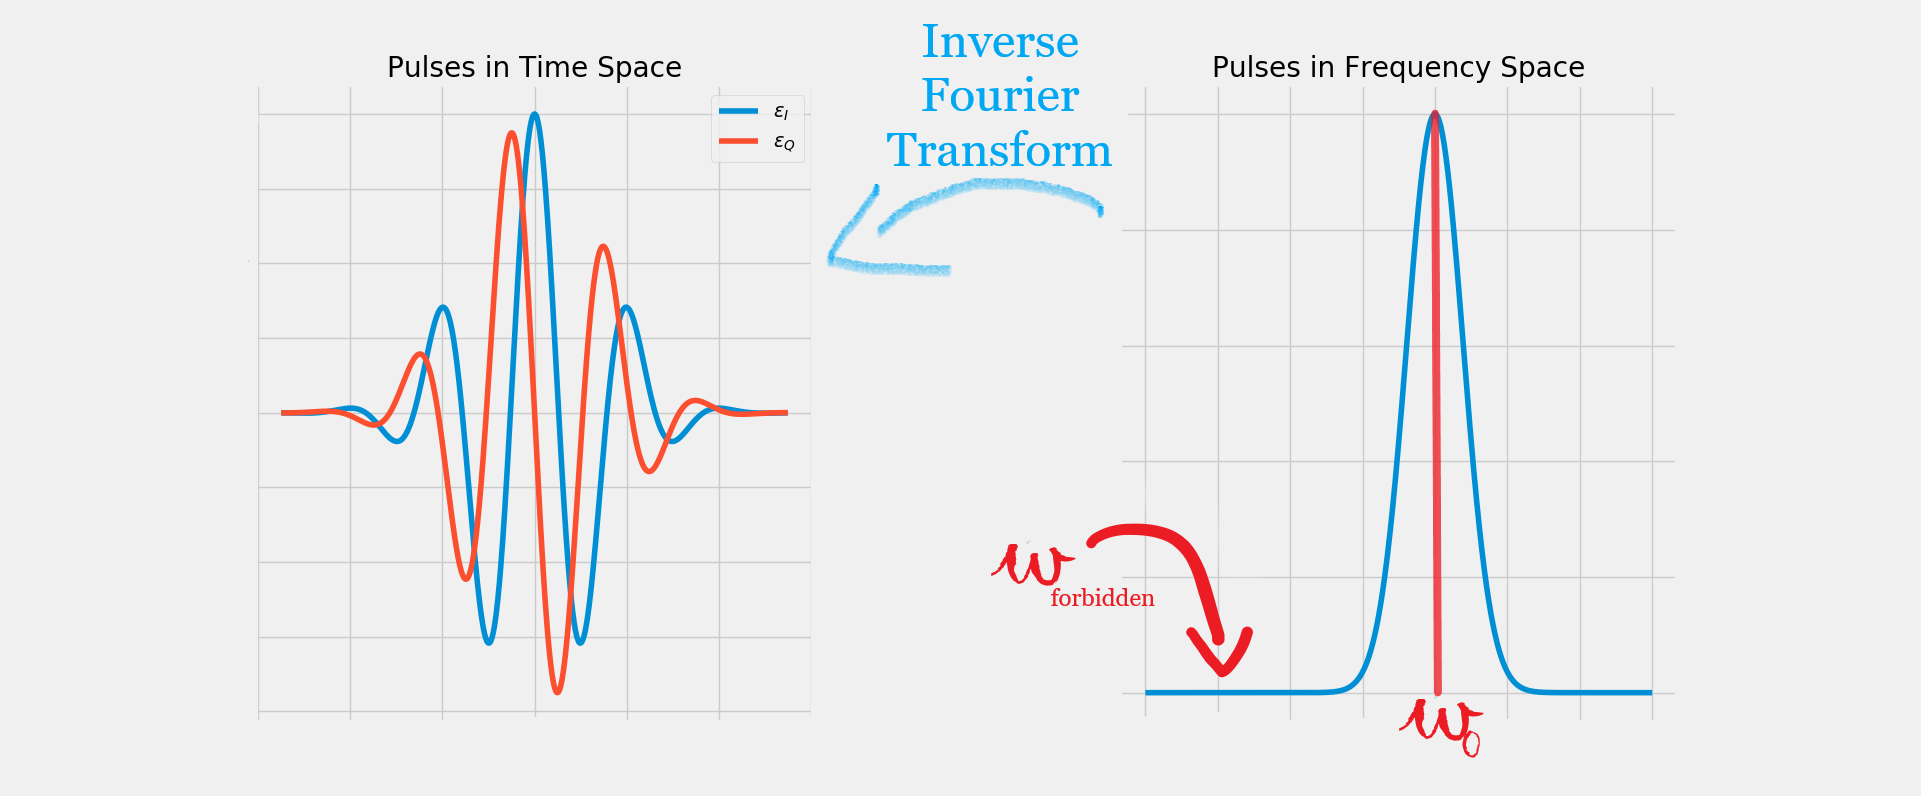
\includegraphics[width=0.9\columnwidth]{gfx/exaple-of-engineered-guess-edited.png}
%     \caption{Example of how you might engineer an initial pulse for a system with known characteristics. Normally you would also add some random noise on top of the pulse}
%     \label{fig:example-engineered-initial-guess}
% \end{figure}
\begin{figure}[H]
    \begin{center}
        %% Creator: Matplotlib, PGF backend
%%
%% To include the figure in your LaTeX document, write
%%   \input{<filename>.pgf}
%%
%% Make sure the required packages are loaded in your preamble
%%   \usepackage{pgf}
%%
%% and, on pdftex
%%   \usepackage[utf8]{inputenc}\DeclareUnicodeCharacter{2212}{-}
%%
%% or, on luatex and xetex
%%   \usepackage{unicode-math}
%%
%% Figures using additional raster images can only be included by \input if
%% they are in the same directory as the main LaTeX file. For loading figures
%% from other directories you can use the `import` package
%%   \usepackage{import}
%%
%% and then include the figures with
%%   \import{<path to file>}{<filename>.pgf}
%%
%% Matplotlib used the following preamble
%%
\begingroup%
\makeatletter%
\begin{pgfpicture}%
\pgfpathrectangle{\pgfpointorigin}{\pgfqpoint{4.650000in}{3.000000in}}%
\pgfusepath{use as bounding box, clip}%
\begin{pgfscope}%
\pgfsetbuttcap%
\pgfsetmiterjoin%
\definecolor{currentfill}{rgb}{1.000000,1.000000,1.000000}%
\pgfsetfillcolor{currentfill}%
\pgfsetlinewidth{0.000000pt}%
\definecolor{currentstroke}{rgb}{1.000000,1.000000,1.000000}%
\pgfsetstrokecolor{currentstroke}%
\pgfsetdash{}{0pt}%
\pgfpathmoveto{\pgfqpoint{0.000000in}{0.000000in}}%
\pgfpathlineto{\pgfqpoint{4.650000in}{0.000000in}}%
\pgfpathlineto{\pgfqpoint{4.650000in}{3.000000in}}%
\pgfpathlineto{\pgfqpoint{0.000000in}{3.000000in}}%
\pgfpathclose%
\pgfusepath{fill}%
\end{pgfscope}%
\begin{pgfscope}%
\pgfsetbuttcap%
\pgfsetmiterjoin%
\definecolor{currentfill}{rgb}{1.000000,1.000000,1.000000}%
\pgfsetfillcolor{currentfill}%
\pgfsetlinewidth{0.000000pt}%
\definecolor{currentstroke}{rgb}{0.000000,0.000000,0.000000}%
\pgfsetstrokecolor{currentstroke}%
\pgfsetstrokeopacity{0.000000}%
\pgfsetdash{}{0pt}%
\pgfpathmoveto{\pgfqpoint{0.308638in}{0.340741in}}%
\pgfpathlineto{\pgfqpoint{2.086318in}{0.340741in}}%
\pgfpathlineto{\pgfqpoint{2.086318in}{2.627778in}}%
\pgfpathlineto{\pgfqpoint{0.308638in}{2.627778in}}%
\pgfpathclose%
\pgfusepath{fill}%
\end{pgfscope}%
\begin{pgfscope}%
\pgfpathrectangle{\pgfqpoint{0.308638in}{0.340741in}}{\pgfqpoint{1.777679in}{2.287037in}}%
\pgfusepath{clip}%
\pgfsetrectcap%
\pgfsetroundjoin%
\pgfsetlinewidth{0.803000pt}%
\definecolor{currentstroke}{rgb}{0.501961,0.501961,0.501961}%
\pgfsetstrokecolor{currentstroke}%
\pgfsetstrokeopacity{0.200000}%
\pgfsetdash{}{0pt}%
\pgfpathmoveto{\pgfqpoint{0.692455in}{0.340741in}}%
\pgfpathlineto{\pgfqpoint{0.692455in}{2.627778in}}%
\pgfusepath{stroke}%
\end{pgfscope}%
\begin{pgfscope}%
\pgfpathrectangle{\pgfqpoint{0.308638in}{0.340741in}}{\pgfqpoint{1.777679in}{2.287037in}}%
\pgfusepath{clip}%
\pgfsetrectcap%
\pgfsetroundjoin%
\pgfsetlinewidth{0.803000pt}%
\definecolor{currentstroke}{rgb}{0.501961,0.501961,0.501961}%
\pgfsetstrokecolor{currentstroke}%
\pgfsetstrokeopacity{0.200000}%
\pgfsetdash{}{0pt}%
\pgfpathmoveto{\pgfqpoint{1.197478in}{0.340741in}}%
\pgfpathlineto{\pgfqpoint{1.197478in}{2.627778in}}%
\pgfusepath{stroke}%
\end{pgfscope}%
\begin{pgfscope}%
\pgfpathrectangle{\pgfqpoint{0.308638in}{0.340741in}}{\pgfqpoint{1.777679in}{2.287037in}}%
\pgfusepath{clip}%
\pgfsetrectcap%
\pgfsetroundjoin%
\pgfsetlinewidth{0.803000pt}%
\definecolor{currentstroke}{rgb}{0.501961,0.501961,0.501961}%
\pgfsetstrokecolor{currentstroke}%
\pgfsetstrokeopacity{0.200000}%
\pgfsetdash{}{0pt}%
\pgfpathmoveto{\pgfqpoint{1.702501in}{0.340741in}}%
\pgfpathlineto{\pgfqpoint{1.702501in}{2.627778in}}%
\pgfusepath{stroke}%
\end{pgfscope}%
\begin{pgfscope}%
\definecolor{textcolor}{rgb}{0.333333,0.333333,0.333333}%
\pgfsetstrokecolor{textcolor}%
\pgfsetfillcolor{textcolor}%
\pgftext[x=1.197478in,y=0.285185in,,top]{\color{textcolor}\rmfamily\fontsize{11.000000}{13.200000}\selectfont time \(\displaystyle t\)}%
\end{pgfscope}%
\begin{pgfscope}%
\pgfpathrectangle{\pgfqpoint{0.308638in}{0.340741in}}{\pgfqpoint{1.777679in}{2.287037in}}%
\pgfusepath{clip}%
\pgfsetrectcap%
\pgfsetroundjoin%
\pgfsetlinewidth{0.803000pt}%
\definecolor{currentstroke}{rgb}{0.501961,0.501961,0.501961}%
\pgfsetstrokecolor{currentstroke}%
\pgfsetstrokeopacity{0.200000}%
\pgfsetdash{}{0pt}%
\pgfpathmoveto{\pgfqpoint{0.308638in}{0.395871in}}%
\pgfpathlineto{\pgfqpoint{2.086318in}{0.395871in}}%
\pgfusepath{stroke}%
\end{pgfscope}%
\begin{pgfscope}%
\pgfpathrectangle{\pgfqpoint{0.308638in}{0.340741in}}{\pgfqpoint{1.777679in}{2.287037in}}%
\pgfusepath{clip}%
\pgfsetrectcap%
\pgfsetroundjoin%
\pgfsetlinewidth{0.803000pt}%
\definecolor{currentstroke}{rgb}{0.501961,0.501961,0.501961}%
\pgfsetstrokecolor{currentstroke}%
\pgfsetstrokeopacity{0.200000}%
\pgfsetdash{}{0pt}%
\pgfpathmoveto{\pgfqpoint{0.308638in}{0.927915in}}%
\pgfpathlineto{\pgfqpoint{2.086318in}{0.927915in}}%
\pgfusepath{stroke}%
\end{pgfscope}%
\begin{pgfscope}%
\pgfpathrectangle{\pgfqpoint{0.308638in}{0.340741in}}{\pgfqpoint{1.777679in}{2.287037in}}%
\pgfusepath{clip}%
\pgfsetrectcap%
\pgfsetroundjoin%
\pgfsetlinewidth{0.803000pt}%
\definecolor{currentstroke}{rgb}{0.501961,0.501961,0.501961}%
\pgfsetstrokecolor{currentstroke}%
\pgfsetstrokeopacity{0.200000}%
\pgfsetdash{}{0pt}%
\pgfpathmoveto{\pgfqpoint{0.308638in}{1.459958in}}%
\pgfpathlineto{\pgfqpoint{2.086318in}{1.459958in}}%
\pgfusepath{stroke}%
\end{pgfscope}%
\begin{pgfscope}%
\pgfpathrectangle{\pgfqpoint{0.308638in}{0.340741in}}{\pgfqpoint{1.777679in}{2.287037in}}%
\pgfusepath{clip}%
\pgfsetrectcap%
\pgfsetroundjoin%
\pgfsetlinewidth{0.803000pt}%
\definecolor{currentstroke}{rgb}{0.501961,0.501961,0.501961}%
\pgfsetstrokecolor{currentstroke}%
\pgfsetstrokeopacity{0.200000}%
\pgfsetdash{}{0pt}%
\pgfpathmoveto{\pgfqpoint{0.308638in}{1.992002in}}%
\pgfpathlineto{\pgfqpoint{2.086318in}{1.992002in}}%
\pgfusepath{stroke}%
\end{pgfscope}%
\begin{pgfscope}%
\pgfpathrectangle{\pgfqpoint{0.308638in}{0.340741in}}{\pgfqpoint{1.777679in}{2.287037in}}%
\pgfusepath{clip}%
\pgfsetrectcap%
\pgfsetroundjoin%
\pgfsetlinewidth{0.803000pt}%
\definecolor{currentstroke}{rgb}{0.501961,0.501961,0.501961}%
\pgfsetstrokecolor{currentstroke}%
\pgfsetstrokeopacity{0.200000}%
\pgfsetdash{}{0pt}%
\pgfpathmoveto{\pgfqpoint{0.308638in}{2.524046in}}%
\pgfpathlineto{\pgfqpoint{2.086318in}{2.524046in}}%
\pgfusepath{stroke}%
\end{pgfscope}%
\begin{pgfscope}%
\pgfsetbuttcap%
\pgfsetmiterjoin%
\definecolor{currentfill}{rgb}{0.000000,0.000000,0.000000}%
\pgfsetfillcolor{currentfill}%
\pgfsetlinewidth{1.003750pt}%
\definecolor{currentstroke}{rgb}{0.000000,0.000000,0.000000}%
\pgfsetstrokecolor{currentstroke}%
\pgfsetdash{}{0pt}%
\pgfpathmoveto{\pgfqpoint{2.005514in}{0.332026in}}%
\pgfpathlineto{\pgfqpoint{1.924711in}{0.278821in}}%
\pgfpathlineto{\pgfqpoint{1.948952in}{0.331494in}}%
\pgfpathlineto{\pgfqpoint{0.389442in}{0.331494in}}%
\pgfpathlineto{\pgfqpoint{0.389442in}{0.332558in}}%
\pgfpathlineto{\pgfqpoint{1.948952in}{0.332558in}}%
\pgfpathlineto{\pgfqpoint{1.924711in}{0.385230in}}%
\pgfpathclose%
\pgfusepath{stroke,fill}%
\end{pgfscope}%
\begin{pgfscope}%
\pgfpathrectangle{\pgfqpoint{0.308638in}{0.340741in}}{\pgfqpoint{1.777679in}{2.287037in}}%
\pgfusepath{clip}%
\pgfsetrectcap%
\pgfsetroundjoin%
\pgfsetlinewidth{1.505625pt}%
\definecolor{currentstroke}{rgb}{0.886275,0.290196,0.200000}%
\pgfsetstrokecolor{currentstroke}%
\pgfsetdash{}{0pt}%
\pgfpathmoveto{\pgfqpoint{0.389442in}{1.459619in}}%
\pgfpathlineto{\pgfqpoint{0.465473in}{1.460848in}}%
\pgfpathlineto{\pgfqpoint{0.543122in}{1.463003in}}%
\pgfpathlineto{\pgfqpoint{0.567388in}{1.459716in}}%
\pgfpathlineto{\pgfqpoint{0.590035in}{1.453489in}}%
\pgfpathlineto{\pgfqpoint{0.643419in}{1.436721in}}%
\pgfpathlineto{\pgfqpoint{0.656361in}{1.436935in}}%
\pgfpathlineto{\pgfqpoint{0.667685in}{1.440216in}}%
\pgfpathlineto{\pgfqpoint{0.679008in}{1.446988in}}%
\pgfpathlineto{\pgfqpoint{0.690332in}{1.457554in}}%
\pgfpathlineto{\pgfqpoint{0.703274in}{1.474153in}}%
\pgfpathlineto{\pgfqpoint{0.721068in}{1.503047in}}%
\pgfpathlineto{\pgfqpoint{0.748569in}{1.548673in}}%
\pgfpathlineto{\pgfqpoint{0.759893in}{1.561247in}}%
\pgfpathlineto{\pgfqpoint{0.767981in}{1.565733in}}%
\pgfpathlineto{\pgfqpoint{0.774452in}{1.565884in}}%
\pgfpathlineto{\pgfqpoint{0.780923in}{1.562502in}}%
\pgfpathlineto{\pgfqpoint{0.787394in}{1.555219in}}%
\pgfpathlineto{\pgfqpoint{0.795482in}{1.540225in}}%
\pgfpathlineto{\pgfqpoint{0.803571in}{1.518442in}}%
\pgfpathlineto{\pgfqpoint{0.813277in}{1.483467in}}%
\pgfpathlineto{\pgfqpoint{0.826218in}{1.423452in}}%
\pgfpathlineto{\pgfqpoint{0.845630in}{1.315010in}}%
\pgfpathlineto{\pgfqpoint{0.866660in}{1.201209in}}%
\pgfpathlineto{\pgfqpoint{0.877984in}{1.156706in}}%
\pgfpathlineto{\pgfqpoint{0.886073in}{1.137447in}}%
\pgfpathlineto{\pgfqpoint{0.890926in}{1.132074in}}%
\pgfpathlineto{\pgfqpoint{0.894161in}{1.131353in}}%
\pgfpathlineto{\pgfqpoint{0.897397in}{1.133057in}}%
\pgfpathlineto{\pgfqpoint{0.902250in}{1.140377in}}%
\pgfpathlineto{\pgfqpoint{0.907103in}{1.153649in}}%
\pgfpathlineto{\pgfqpoint{0.913573in}{1.180891in}}%
\pgfpathlineto{\pgfqpoint{0.921662in}{1.230400in}}%
\pgfpathlineto{\pgfqpoint{0.931368in}{1.311627in}}%
\pgfpathlineto{\pgfqpoint{0.944310in}{1.452024in}}%
\pgfpathlineto{\pgfqpoint{0.963722in}{1.705064in}}%
\pgfpathlineto{\pgfqpoint{0.984752in}{1.970919in}}%
\pgfpathlineto{\pgfqpoint{0.996076in}{2.078564in}}%
\pgfpathlineto{\pgfqpoint{1.004164in}{2.129906in}}%
\pgfpathlineto{\pgfqpoint{1.010635in}{2.152335in}}%
\pgfpathlineto{\pgfqpoint{1.013870in}{2.156726in}}%
\pgfpathlineto{\pgfqpoint{1.017106in}{2.156337in}}%
\pgfpathlineto{\pgfqpoint{1.020341in}{2.151035in}}%
\pgfpathlineto{\pgfqpoint{1.025194in}{2.133672in}}%
\pgfpathlineto{\pgfqpoint{1.031665in}{2.092750in}}%
\pgfpathlineto{\pgfqpoint{1.039753in}{2.013383in}}%
\pgfpathlineto{\pgfqpoint{1.049459in}{1.879304in}}%
\pgfpathlineto{\pgfqpoint{1.060783in}{1.677337in}}%
\pgfpathlineto{\pgfqpoint{1.078578in}{1.297093in}}%
\pgfpathlineto{\pgfqpoint{1.102843in}{0.784777in}}%
\pgfpathlineto{\pgfqpoint{1.114167in}{0.603305in}}%
\pgfpathlineto{\pgfqpoint{1.122255in}{0.511767in}}%
\pgfpathlineto{\pgfqpoint{1.128726in}{0.465565in}}%
\pgfpathlineto{\pgfqpoint{1.133579in}{0.447982in}}%
\pgfpathlineto{\pgfqpoint{1.136815in}{0.444697in}}%
\pgfpathlineto{\pgfqpoint{1.140050in}{0.448273in}}%
\pgfpathlineto{\pgfqpoint{1.143285in}{0.458746in}}%
\pgfpathlineto{\pgfqpoint{1.148138in}{0.487335in}}%
\pgfpathlineto{\pgfqpoint{1.154609in}{0.548979in}}%
\pgfpathlineto{\pgfqpoint{1.162698in}{0.661708in}}%
\pgfpathlineto{\pgfqpoint{1.172404in}{0.843070in}}%
\pgfpathlineto{\pgfqpoint{1.186963in}{1.185086in}}%
\pgfpathlineto{\pgfqpoint{1.225788in}{2.142320in}}%
\pgfpathlineto{\pgfqpoint{1.237111in}{2.330416in}}%
\pgfpathlineto{\pgfqpoint{1.245200in}{2.419657in}}%
\pgfpathlineto{\pgfqpoint{1.251671in}{2.461170in}}%
\pgfpathlineto{\pgfqpoint{1.256524in}{2.474293in}}%
\pgfpathlineto{\pgfqpoint{1.259759in}{2.474431in}}%
\pgfpathlineto{\pgfqpoint{1.262994in}{2.467746in}}%
\pgfpathlineto{\pgfqpoint{1.267848in}{2.445189in}}%
\pgfpathlineto{\pgfqpoint{1.274318in}{2.392722in}}%
\pgfpathlineto{\pgfqpoint{1.282407in}{2.294199in}}%
\pgfpathlineto{\pgfqpoint{1.292113in}{2.135140in}}%
\pgfpathlineto{\pgfqpoint{1.306672in}{1.838683in}}%
\pgfpathlineto{\pgfqpoint{1.340644in}{1.121846in}}%
\pgfpathlineto{\pgfqpoint{1.351967in}{0.946729in}}%
\pgfpathlineto{\pgfqpoint{1.361674in}{0.840562in}}%
\pgfpathlineto{\pgfqpoint{1.369762in}{0.786245in}}%
\pgfpathlineto{\pgfqpoint{1.374615in}{0.768882in}}%
\pgfpathlineto{\pgfqpoint{1.377850in}{0.763580in}}%
\pgfpathlineto{\pgfqpoint{1.381086in}{0.763190in}}%
\pgfpathlineto{\pgfqpoint{1.384321in}{0.767581in}}%
\pgfpathlineto{\pgfqpoint{1.389174in}{0.782760in}}%
\pgfpathlineto{\pgfqpoint{1.395645in}{0.817929in}}%
\pgfpathlineto{\pgfqpoint{1.403733in}{0.882990in}}%
\pgfpathlineto{\pgfqpoint{1.415057in}{1.004913in}}%
\pgfpathlineto{\pgfqpoint{1.434470in}{1.258565in}}%
\pgfpathlineto{\pgfqpoint{1.455500in}{1.524290in}}%
\pgfpathlineto{\pgfqpoint{1.468441in}{1.651762in}}%
\pgfpathlineto{\pgfqpoint{1.478147in}{1.721272in}}%
\pgfpathlineto{\pgfqpoint{1.486236in}{1.760488in}}%
\pgfpathlineto{\pgfqpoint{1.492706in}{1.779540in}}%
\pgfpathlineto{\pgfqpoint{1.497560in}{1.786860in}}%
\pgfpathlineto{\pgfqpoint{1.502413in}{1.788500in}}%
\pgfpathlineto{\pgfqpoint{1.505648in}{1.786608in}}%
\pgfpathlineto{\pgfqpoint{1.510501in}{1.779600in}}%
\pgfpathlineto{\pgfqpoint{1.516972in}{1.763211in}}%
\pgfpathlineto{\pgfqpoint{1.525060in}{1.733163in}}%
\pgfpathlineto{\pgfqpoint{1.536384in}{1.678000in}}%
\pgfpathlineto{\pgfqpoint{1.584915in}{1.423754in}}%
\pgfpathlineto{\pgfqpoint{1.596239in}{1.387586in}}%
\pgfpathlineto{\pgfqpoint{1.605945in}{1.367162in}}%
\pgfpathlineto{\pgfqpoint{1.614033in}{1.357415in}}%
\pgfpathlineto{\pgfqpoint{1.620504in}{1.354033in}}%
\pgfpathlineto{\pgfqpoint{1.626975in}{1.354184in}}%
\pgfpathlineto{\pgfqpoint{1.633445in}{1.357431in}}%
\pgfpathlineto{\pgfqpoint{1.641534in}{1.365100in}}%
\pgfpathlineto{\pgfqpoint{1.652858in}{1.380784in}}%
\pgfpathlineto{\pgfqpoint{1.675505in}{1.419683in}}%
\pgfpathlineto{\pgfqpoint{1.694918in}{1.450333in}}%
\pgfpathlineto{\pgfqpoint{1.707859in}{1.465773in}}%
\pgfpathlineto{\pgfqpoint{1.719183in}{1.475244in}}%
\pgfpathlineto{\pgfqpoint{1.730507in}{1.480973in}}%
\pgfpathlineto{\pgfqpoint{1.741831in}{1.483354in}}%
\pgfpathlineto{\pgfqpoint{1.754772in}{1.482777in}}%
\pgfpathlineto{\pgfqpoint{1.770949in}{1.478716in}}%
\pgfpathlineto{\pgfqpoint{1.835657in}{1.458721in}}%
\pgfpathlineto{\pgfqpoint{1.859922in}{1.456515in}}%
\pgfpathlineto{\pgfqpoint{1.892276in}{1.457086in}}%
\pgfpathlineto{\pgfqpoint{1.986102in}{1.460323in}}%
\pgfpathlineto{\pgfqpoint{2.005514in}{1.460298in}}%
\pgfpathlineto{\pgfqpoint{2.005514in}{1.460298in}}%
\pgfusepath{stroke}%
\end{pgfscope}%
\begin{pgfscope}%
\pgfpathrectangle{\pgfqpoint{0.308638in}{0.340741in}}{\pgfqpoint{1.777679in}{2.287037in}}%
\pgfusepath{clip}%
\pgfsetrectcap%
\pgfsetroundjoin%
\pgfsetlinewidth{1.505625pt}%
\definecolor{currentstroke}{rgb}{0.203922,0.541176,0.741176}%
\pgfsetstrokecolor{currentstroke}%
\pgfsetdash{}{0pt}%
\pgfpathmoveto{\pgfqpoint{0.389442in}{1.460069in}}%
\pgfpathlineto{\pgfqpoint{0.504298in}{1.459868in}}%
\pgfpathlineto{\pgfqpoint{0.541505in}{1.455497in}}%
\pgfpathlineto{\pgfqpoint{0.585182in}{1.450372in}}%
\pgfpathlineto{\pgfqpoint{0.602977in}{1.451420in}}%
\pgfpathlineto{\pgfqpoint{0.619154in}{1.455533in}}%
\pgfpathlineto{\pgfqpoint{0.633713in}{1.462318in}}%
\pgfpathlineto{\pgfqpoint{0.649890in}{1.473179in}}%
\pgfpathlineto{\pgfqpoint{0.700038in}{1.510364in}}%
\pgfpathlineto{\pgfqpoint{0.709745in}{1.512397in}}%
\pgfpathlineto{\pgfqpoint{0.717833in}{1.511214in}}%
\pgfpathlineto{\pgfqpoint{0.725921in}{1.506909in}}%
\pgfpathlineto{\pgfqpoint{0.734010in}{1.499107in}}%
\pgfpathlineto{\pgfqpoint{0.743716in}{1.484804in}}%
\pgfpathlineto{\pgfqpoint{0.755040in}{1.461266in}}%
\pgfpathlineto{\pgfqpoint{0.767981in}{1.426251in}}%
\pgfpathlineto{\pgfqpoint{0.789011in}{1.358128in}}%
\pgfpathlineto{\pgfqpoint{0.808424in}{1.298838in}}%
\pgfpathlineto{\pgfqpoint{0.818130in}{1.277494in}}%
\pgfpathlineto{\pgfqpoint{0.826218in}{1.266802in}}%
\pgfpathlineto{\pgfqpoint{0.831071in}{1.264206in}}%
\pgfpathlineto{\pgfqpoint{0.835924in}{1.264856in}}%
\pgfpathlineto{\pgfqpoint{0.840777in}{1.269025in}}%
\pgfpathlineto{\pgfqpoint{0.847248in}{1.280437in}}%
\pgfpathlineto{\pgfqpoint{0.853719in}{1.298877in}}%
\pgfpathlineto{\pgfqpoint{0.861807in}{1.332053in}}%
\pgfpathlineto{\pgfqpoint{0.871513in}{1.386406in}}%
\pgfpathlineto{\pgfqpoint{0.882837in}{1.467817in}}%
\pgfpathlineto{\pgfqpoint{0.900632in}{1.622900in}}%
\pgfpathlineto{\pgfqpoint{0.926515in}{1.847936in}}%
\pgfpathlineto{\pgfqpoint{0.937839in}{1.918514in}}%
\pgfpathlineto{\pgfqpoint{0.945927in}{1.949892in}}%
\pgfpathlineto{\pgfqpoint{0.950780in}{1.959496in}}%
\pgfpathlineto{\pgfqpoint{0.954016in}{1.961681in}}%
\pgfpathlineto{\pgfqpoint{0.957251in}{1.960317in}}%
\pgfpathlineto{\pgfqpoint{0.960486in}{1.955281in}}%
\pgfpathlineto{\pgfqpoint{0.965340in}{1.940637in}}%
\pgfpathlineto{\pgfqpoint{0.971810in}{1.907581in}}%
\pgfpathlineto{\pgfqpoint{0.979899in}{1.844477in}}%
\pgfpathlineto{\pgfqpoint{0.989605in}{1.738210in}}%
\pgfpathlineto{\pgfqpoint{1.000929in}{1.577522in}}%
\pgfpathlineto{\pgfqpoint{1.018723in}{1.271918in}}%
\pgfpathlineto{\pgfqpoint{1.044606in}{0.829766in}}%
\pgfpathlineto{\pgfqpoint{1.055930in}{0.687043in}}%
\pgfpathlineto{\pgfqpoint{1.064019in}{0.618207in}}%
\pgfpathlineto{\pgfqpoint{1.070489in}{0.586798in}}%
\pgfpathlineto{\pgfqpoint{1.073725in}{0.579638in}}%
\pgfpathlineto{\pgfqpoint{1.076960in}{0.578408in}}%
\pgfpathlineto{\pgfqpoint{1.080195in}{0.583228in}}%
\pgfpathlineto{\pgfqpoint{1.085049in}{0.601953in}}%
\pgfpathlineto{\pgfqpoint{1.089902in}{0.634505in}}%
\pgfpathlineto{\pgfqpoint{1.096372in}{0.699052in}}%
\pgfpathlineto{\pgfqpoint{1.104461in}{0.811996in}}%
\pgfpathlineto{\pgfqpoint{1.115785in}{1.022927in}}%
\pgfpathlineto{\pgfqpoint{1.130344in}{1.359747in}}%
\pgfpathlineto{\pgfqpoint{1.164315in}{2.172200in}}%
\pgfpathlineto{\pgfqpoint{1.175639in}{2.365457in}}%
\pgfpathlineto{\pgfqpoint{1.183728in}{2.460048in}}%
\pgfpathlineto{\pgfqpoint{1.190198in}{2.505957in}}%
\pgfpathlineto{\pgfqpoint{1.195051in}{2.522030in}}%
\pgfpathlineto{\pgfqpoint{1.198287in}{2.523822in}}%
\pgfpathlineto{\pgfqpoint{1.201522in}{2.518450in}}%
\pgfpathlineto{\pgfqpoint{1.206375in}{2.497069in}}%
\pgfpathlineto{\pgfqpoint{1.212846in}{2.444336in}}%
\pgfpathlineto{\pgfqpoint{1.220935in}{2.341920in}}%
\pgfpathlineto{\pgfqpoint{1.230641in}{2.172200in}}%
\pgfpathlineto{\pgfqpoint{1.243582in}{1.886098in}}%
\pgfpathlineto{\pgfqpoint{1.287260in}{0.866451in}}%
\pgfpathlineto{\pgfqpoint{1.296966in}{0.718857in}}%
\pgfpathlineto{\pgfqpoint{1.305054in}{0.634505in}}%
\pgfpathlineto{\pgfqpoint{1.311525in}{0.594173in}}%
\pgfpathlineto{\pgfqpoint{1.316378in}{0.580056in}}%
\pgfpathlineto{\pgfqpoint{1.319614in}{0.578273in}}%
\pgfpathlineto{\pgfqpoint{1.322849in}{0.582486in}}%
\pgfpathlineto{\pgfqpoint{1.327702in}{0.599723in}}%
\pgfpathlineto{\pgfqpoint{1.334173in}{0.642006in}}%
\pgfpathlineto{\pgfqpoint{1.342261in}{0.722824in}}%
\pgfpathlineto{\pgfqpoint{1.351967in}{0.853756in}}%
\pgfpathlineto{\pgfqpoint{1.366527in}{1.096581in}}%
\pgfpathlineto{\pgfqpoint{1.398880in}{1.650682in}}%
\pgfpathlineto{\pgfqpoint{1.410204in}{1.795332in}}%
\pgfpathlineto{\pgfqpoint{1.419910in}{1.885220in}}%
\pgfpathlineto{\pgfqpoint{1.427999in}{1.933831in}}%
\pgfpathlineto{\pgfqpoint{1.434470in}{1.955281in}}%
\pgfpathlineto{\pgfqpoint{1.439323in}{1.961451in}}%
\pgfpathlineto{\pgfqpoint{1.442558in}{1.961023in}}%
\pgfpathlineto{\pgfqpoint{1.445793in}{1.957118in}}%
\pgfpathlineto{\pgfqpoint{1.450646in}{1.945089in}}%
\pgfpathlineto{\pgfqpoint{1.457117in}{1.918514in}}%
\pgfpathlineto{\pgfqpoint{1.465206in}{1.870784in}}%
\pgfpathlineto{\pgfqpoint{1.476530in}{1.783629in}}%
\pgfpathlineto{\pgfqpoint{1.526678in}{1.366587in}}%
\pgfpathlineto{\pgfqpoint{1.536384in}{1.317432in}}%
\pgfpathlineto{\pgfqpoint{1.544473in}{1.288763in}}%
\pgfpathlineto{\pgfqpoint{1.552561in}{1.271237in}}%
\pgfpathlineto{\pgfqpoint{1.559032in}{1.264856in}}%
\pgfpathlineto{\pgfqpoint{1.563885in}{1.264206in}}%
\pgfpathlineto{\pgfqpoint{1.568738in}{1.266802in}}%
\pgfpathlineto{\pgfqpoint{1.575209in}{1.274777in}}%
\pgfpathlineto{\pgfqpoint{1.583297in}{1.290853in}}%
\pgfpathlineto{\pgfqpoint{1.594621in}{1.321722in}}%
\pgfpathlineto{\pgfqpoint{1.618886in}{1.401020in}}%
\pgfpathlineto{\pgfqpoint{1.636681in}{1.453257in}}%
\pgfpathlineto{\pgfqpoint{1.649622in}{1.481887in}}%
\pgfpathlineto{\pgfqpoint{1.659328in}{1.497103in}}%
\pgfpathlineto{\pgfqpoint{1.669035in}{1.506909in}}%
\pgfpathlineto{\pgfqpoint{1.677123in}{1.511214in}}%
\pgfpathlineto{\pgfqpoint{1.685212in}{1.512397in}}%
\pgfpathlineto{\pgfqpoint{1.694918in}{1.510364in}}%
\pgfpathlineto{\pgfqpoint{1.706242in}{1.504395in}}%
\pgfpathlineto{\pgfqpoint{1.724036in}{1.490578in}}%
\pgfpathlineto{\pgfqpoint{1.754772in}{1.466277in}}%
\pgfpathlineto{\pgfqpoint{1.770949in}{1.457460in}}%
\pgfpathlineto{\pgfqpoint{1.787126in}{1.452298in}}%
\pgfpathlineto{\pgfqpoint{1.803303in}{1.450401in}}%
\pgfpathlineto{\pgfqpoint{1.824333in}{1.451381in}}%
\pgfpathlineto{\pgfqpoint{1.924630in}{1.461148in}}%
\pgfpathlineto{\pgfqpoint{2.005514in}{1.460069in}}%
\pgfpathlineto{\pgfqpoint{2.005514in}{1.460069in}}%
\pgfusepath{stroke}%
\end{pgfscope}%
\begin{pgfscope}%
\pgfsetrectcap%
\pgfsetmiterjoin%
\pgfsetlinewidth{1.003750pt}%
\definecolor{currentstroke}{rgb}{1.000000,1.000000,1.000000}%
\pgfsetstrokecolor{currentstroke}%
\pgfsetdash{}{0pt}%
\pgfpathmoveto{\pgfqpoint{0.308638in}{0.340741in}}%
\pgfpathlineto{\pgfqpoint{0.308638in}{2.627778in}}%
\pgfusepath{stroke}%
\end{pgfscope}%
\begin{pgfscope}%
\pgfsetrectcap%
\pgfsetmiterjoin%
\pgfsetlinewidth{1.003750pt}%
\definecolor{currentstroke}{rgb}{1.000000,1.000000,1.000000}%
\pgfsetstrokecolor{currentstroke}%
\pgfsetdash{}{0pt}%
\pgfpathmoveto{\pgfqpoint{2.086318in}{0.340741in}}%
\pgfpathlineto{\pgfqpoint{2.086318in}{2.627778in}}%
\pgfusepath{stroke}%
\end{pgfscope}%
\begin{pgfscope}%
\pgfsetrectcap%
\pgfsetmiterjoin%
\pgfsetlinewidth{1.003750pt}%
\definecolor{currentstroke}{rgb}{1.000000,1.000000,1.000000}%
\pgfsetstrokecolor{currentstroke}%
\pgfsetdash{}{0pt}%
\pgfpathmoveto{\pgfqpoint{0.308638in}{0.340741in}}%
\pgfpathlineto{\pgfqpoint{2.086318in}{0.340741in}}%
\pgfusepath{stroke}%
\end{pgfscope}%
\begin{pgfscope}%
\pgfsetrectcap%
\pgfsetmiterjoin%
\pgfsetlinewidth{1.003750pt}%
\definecolor{currentstroke}{rgb}{1.000000,1.000000,1.000000}%
\pgfsetstrokecolor{currentstroke}%
\pgfsetdash{}{0pt}%
\pgfpathmoveto{\pgfqpoint{0.308638in}{2.627778in}}%
\pgfpathlineto{\pgfqpoint{2.086318in}{2.627778in}}%
\pgfusepath{stroke}%
\end{pgfscope}%
\begin{pgfscope}%
\pgfsetroundcap%
\pgfsetroundjoin%
\definecolor{currentfill}{rgb}{0.000000,0.000000,0.000000}%
\pgfsetfillcolor{currentfill}%
\pgfsetlinewidth{0.501875pt}%
\definecolor{currentstroke}{rgb}{0.933333,0.933333,0.933333}%
\pgfsetstrokecolor{currentstroke}%
\pgfsetdash{}{0pt}%
\pgfpathmoveto{\pgfqpoint{2.458013in}{2.090688in}}%
\pgfpathquadraticcurveto{\pgfqpoint{2.108124in}{2.232358in}}{\pgfqpoint{1.793530in}{2.079649in}}%
\pgfpathlineto{\pgfqpoint{1.817791in}{2.029671in}}%
\pgfpathquadraticcurveto{\pgfqpoint{1.733460in}{2.035394in}}{\pgfqpoint{1.638282in}{2.019253in}}%
\pgfpathquadraticcurveto{\pgfqpoint{1.684459in}{2.103555in}}{\pgfqpoint{1.745009in}{2.179606in}}%
\pgfpathlineto{\pgfqpoint{1.769270in}{2.129628in}}%
\pgfpathquadraticcurveto{\pgfqpoint{2.106082in}{2.293121in}}{\pgfqpoint{2.478863in}{2.142183in}}%
\pgfpathlineto{\pgfqpoint{2.458013in}{2.090688in}}%
\pgfpathclose%
\pgfusepath{stroke,fill}%
\end{pgfscope}%
\begin{pgfscope}%
\definecolor{textcolor}{rgb}{0.000000,0.000000,0.000000}%
\pgfsetstrokecolor{textcolor}%
\pgfsetfillcolor{textcolor}%
\pgftext[x=1.803505in, y=1.908958in, left, base]{\color{textcolor}\rmfamily\fontsize{12.000000}{14.400000}\selectfont Inverse}%
\end{pgfscope}%
\begin{pgfscope}%
\definecolor{textcolor}{rgb}{0.000000,0.000000,0.000000}%
\pgfsetstrokecolor{textcolor}%
\pgfsetfillcolor{textcolor}%
\pgftext[x=1.803505in, y=1.737663in, left, base]{\color{textcolor}\rmfamily\fontsize{12.000000}{14.400000}\selectfont Fourier}%
\end{pgfscope}%
\begin{pgfscope}%
\definecolor{textcolor}{rgb}{0.000000,0.000000,0.000000}%
\pgfsetstrokecolor{textcolor}%
\pgfsetfillcolor{textcolor}%
\pgftext[x=1.803505in, y=1.566367in, left, base]{\color{textcolor}\rmfamily\fontsize{12.000000}{14.400000}\selectfont Transform}%
\end{pgfscope}%
\begin{pgfscope}%
\definecolor{textcolor}{rgb}{0.000000,0.000000,0.000000}%
\pgfsetstrokecolor{textcolor}%
\pgfsetfillcolor{textcolor}%
\pgftext[x=1.197478in,y=2.711111in,,base]{\color{textcolor}\rmfamily\fontsize{14.000000}{16.800000}\selectfont Time space}%
\end{pgfscope}%
\begin{pgfscope}%
\pgfsetbuttcap%
\pgfsetmiterjoin%
\definecolor{currentfill}{rgb}{1.000000,1.000000,1.000000}%
\pgfsetfillcolor{currentfill}%
\pgfsetfillopacity{0.800000}%
\pgfsetlinewidth{0.501875pt}%
\definecolor{currentstroke}{rgb}{0.800000,0.800000,0.800000}%
\pgfsetstrokecolor{currentstroke}%
\pgfsetstrokeopacity{0.800000}%
\pgfsetdash{}{0pt}%
\pgfpathmoveto{\pgfqpoint{0.148931in}{2.068745in}}%
\pgfpathlineto{\pgfqpoint{0.799351in}{2.068745in}}%
\pgfpathquadraticcurveto{\pgfqpoint{0.829907in}{2.068745in}}{\pgfqpoint{0.829907in}{2.099300in}}%
\pgfpathlineto{\pgfqpoint{0.829907in}{2.525408in}}%
\pgfpathquadraticcurveto{\pgfqpoint{0.829907in}{2.555963in}}{\pgfqpoint{0.799351in}{2.555963in}}%
\pgfpathlineto{\pgfqpoint{0.148931in}{2.555963in}}%
\pgfpathquadraticcurveto{\pgfqpoint{0.118375in}{2.555963in}}{\pgfqpoint{0.118375in}{2.525408in}}%
\pgfpathlineto{\pgfqpoint{0.118375in}{2.099300in}}%
\pgfpathquadraticcurveto{\pgfqpoint{0.118375in}{2.068745in}}{\pgfqpoint{0.148931in}{2.068745in}}%
\pgfpathclose%
\pgfusepath{stroke,fill}%
\end{pgfscope}%
\begin{pgfscope}%
\pgfsetrectcap%
\pgfsetroundjoin%
\pgfsetlinewidth{1.505625pt}%
\definecolor{currentstroke}{rgb}{0.886275,0.290196,0.200000}%
\pgfsetstrokecolor{currentstroke}%
\pgfsetdash{}{0pt}%
\pgfpathmoveto{\pgfqpoint{0.179486in}{2.441380in}}%
\pgfpathlineto{\pgfqpoint{0.485042in}{2.441380in}}%
\pgfusepath{stroke}%
\end{pgfscope}%
\begin{pgfscope}%
\definecolor{textcolor}{rgb}{0.000000,0.000000,0.000000}%
\pgfsetstrokecolor{textcolor}%
\pgfsetfillcolor{textcolor}%
\pgftext[x=0.607264in,y=2.387908in,left,base]{\color{textcolor}\rmfamily\fontsize{11.000000}{13.200000}\selectfont \(\displaystyle \epsilon_I\)}%
\end{pgfscope}%
\begin{pgfscope}%
\pgfsetrectcap%
\pgfsetroundjoin%
\pgfsetlinewidth{1.505625pt}%
\definecolor{currentstroke}{rgb}{0.203922,0.541176,0.741176}%
\pgfsetstrokecolor{currentstroke}%
\pgfsetdash{}{0pt}%
\pgfpathmoveto{\pgfqpoint{0.179486in}{2.228475in}}%
\pgfpathlineto{\pgfqpoint{0.485042in}{2.228475in}}%
\pgfusepath{stroke}%
\end{pgfscope}%
\begin{pgfscope}%
\definecolor{textcolor}{rgb}{0.000000,0.000000,0.000000}%
\pgfsetstrokecolor{textcolor}%
\pgfsetfillcolor{textcolor}%
\pgftext[x=0.607264in,y=2.175003in,left,base]{\color{textcolor}\rmfamily\fontsize{11.000000}{13.200000}\selectfont \(\displaystyle \epsilon_Q\)}%
\end{pgfscope}%
\begin{pgfscope}%
\pgfsetbuttcap%
\pgfsetmiterjoin%
\definecolor{currentfill}{rgb}{1.000000,1.000000,1.000000}%
\pgfsetfillcolor{currentfill}%
\pgfsetlinewidth{0.000000pt}%
\definecolor{currentstroke}{rgb}{0.000000,0.000000,0.000000}%
\pgfsetstrokecolor{currentstroke}%
\pgfsetstrokeopacity{0.000000}%
\pgfsetdash{}{0pt}%
\pgfpathmoveto{\pgfqpoint{2.722321in}{0.340741in}}%
\pgfpathlineto{\pgfqpoint{4.500000in}{0.340741in}}%
\pgfpathlineto{\pgfqpoint{4.500000in}{2.627778in}}%
\pgfpathlineto{\pgfqpoint{2.722321in}{2.627778in}}%
\pgfpathclose%
\pgfusepath{fill}%
\end{pgfscope}%
\begin{pgfscope}%
\pgfpathrectangle{\pgfqpoint{2.722321in}{0.340741in}}{\pgfqpoint{1.777679in}{2.287037in}}%
\pgfusepath{clip}%
\pgfsetrectcap%
\pgfsetroundjoin%
\pgfsetlinewidth{0.803000pt}%
\definecolor{currentstroke}{rgb}{0.501961,0.501961,0.501961}%
\pgfsetstrokecolor{currentstroke}%
\pgfsetstrokeopacity{0.200000}%
\pgfsetdash{}{0pt}%
\pgfpathmoveto{\pgfqpoint{2.803124in}{0.340741in}}%
\pgfpathlineto{\pgfqpoint{2.803124in}{2.627778in}}%
\pgfusepath{stroke}%
\end{pgfscope}%
\begin{pgfscope}%
\pgfpathrectangle{\pgfqpoint{2.722321in}{0.340741in}}{\pgfqpoint{1.777679in}{2.287037in}}%
\pgfusepath{clip}%
\pgfsetrectcap%
\pgfsetroundjoin%
\pgfsetlinewidth{0.803000pt}%
\definecolor{currentstroke}{rgb}{0.501961,0.501961,0.501961}%
\pgfsetstrokecolor{currentstroke}%
\pgfsetstrokeopacity{0.200000}%
\pgfsetdash{}{0pt}%
\pgfpathmoveto{\pgfqpoint{3.611160in}{0.340741in}}%
\pgfpathlineto{\pgfqpoint{3.611160in}{2.627778in}}%
\pgfusepath{stroke}%
\end{pgfscope}%
\begin{pgfscope}%
\pgfpathrectangle{\pgfqpoint{2.722321in}{0.340741in}}{\pgfqpoint{1.777679in}{2.287037in}}%
\pgfusepath{clip}%
\pgfsetrectcap%
\pgfsetroundjoin%
\pgfsetlinewidth{0.803000pt}%
\definecolor{currentstroke}{rgb}{0.501961,0.501961,0.501961}%
\pgfsetstrokecolor{currentstroke}%
\pgfsetstrokeopacity{0.200000}%
\pgfsetdash{}{0pt}%
\pgfpathmoveto{\pgfqpoint{4.419196in}{0.340741in}}%
\pgfpathlineto{\pgfqpoint{4.419196in}{2.627778in}}%
\pgfusepath{stroke}%
\end{pgfscope}%
\begin{pgfscope}%
\definecolor{textcolor}{rgb}{0.333333,0.333333,0.333333}%
\pgfsetstrokecolor{textcolor}%
\pgfsetfillcolor{textcolor}%
\pgftext[x=3.611160in,y=0.285185in,,top]{\color{textcolor}\rmfamily\fontsize{11.000000}{13.200000}\selectfont Frequency \(\displaystyle \omega\)}%
\end{pgfscope}%
\begin{pgfscope}%
\pgfpathrectangle{\pgfqpoint{2.722321in}{0.340741in}}{\pgfqpoint{1.777679in}{2.287037in}}%
\pgfusepath{clip}%
\pgfsetrectcap%
\pgfsetroundjoin%
\pgfsetlinewidth{0.803000pt}%
\definecolor{currentstroke}{rgb}{0.501961,0.501961,0.501961}%
\pgfsetstrokecolor{currentstroke}%
\pgfsetstrokeopacity{0.200000}%
\pgfsetdash{}{0pt}%
\pgfpathmoveto{\pgfqpoint{2.722321in}{0.444697in}}%
\pgfpathlineto{\pgfqpoint{4.500000in}{0.444697in}}%
\pgfusepath{stroke}%
\end{pgfscope}%
\begin{pgfscope}%
\pgfpathrectangle{\pgfqpoint{2.722321in}{0.340741in}}{\pgfqpoint{1.777679in}{2.287037in}}%
\pgfusepath{clip}%
\pgfsetrectcap%
\pgfsetroundjoin%
\pgfsetlinewidth{0.803000pt}%
\definecolor{currentstroke}{rgb}{0.501961,0.501961,0.501961}%
\pgfsetstrokecolor{currentstroke}%
\pgfsetstrokeopacity{0.200000}%
\pgfsetdash{}{0pt}%
\pgfpathmoveto{\pgfqpoint{2.722321in}{0.860522in}}%
\pgfpathlineto{\pgfqpoint{4.500000in}{0.860522in}}%
\pgfusepath{stroke}%
\end{pgfscope}%
\begin{pgfscope}%
\pgfpathrectangle{\pgfqpoint{2.722321in}{0.340741in}}{\pgfqpoint{1.777679in}{2.287037in}}%
\pgfusepath{clip}%
\pgfsetrectcap%
\pgfsetroundjoin%
\pgfsetlinewidth{0.803000pt}%
\definecolor{currentstroke}{rgb}{0.501961,0.501961,0.501961}%
\pgfsetstrokecolor{currentstroke}%
\pgfsetstrokeopacity{0.200000}%
\pgfsetdash{}{0pt}%
\pgfpathmoveto{\pgfqpoint{2.722321in}{1.276347in}}%
\pgfpathlineto{\pgfqpoint{4.500000in}{1.276347in}}%
\pgfusepath{stroke}%
\end{pgfscope}%
\begin{pgfscope}%
\pgfpathrectangle{\pgfqpoint{2.722321in}{0.340741in}}{\pgfqpoint{1.777679in}{2.287037in}}%
\pgfusepath{clip}%
\pgfsetrectcap%
\pgfsetroundjoin%
\pgfsetlinewidth{0.803000pt}%
\definecolor{currentstroke}{rgb}{0.501961,0.501961,0.501961}%
\pgfsetstrokecolor{currentstroke}%
\pgfsetstrokeopacity{0.200000}%
\pgfsetdash{}{0pt}%
\pgfpathmoveto{\pgfqpoint{2.722321in}{1.692172in}}%
\pgfpathlineto{\pgfqpoint{4.500000in}{1.692172in}}%
\pgfusepath{stroke}%
\end{pgfscope}%
\begin{pgfscope}%
\pgfpathrectangle{\pgfqpoint{2.722321in}{0.340741in}}{\pgfqpoint{1.777679in}{2.287037in}}%
\pgfusepath{clip}%
\pgfsetrectcap%
\pgfsetroundjoin%
\pgfsetlinewidth{0.803000pt}%
\definecolor{currentstroke}{rgb}{0.501961,0.501961,0.501961}%
\pgfsetstrokecolor{currentstroke}%
\pgfsetstrokeopacity{0.200000}%
\pgfsetdash{}{0pt}%
\pgfpathmoveto{\pgfqpoint{2.722321in}{2.107997in}}%
\pgfpathlineto{\pgfqpoint{4.500000in}{2.107997in}}%
\pgfusepath{stroke}%
\end{pgfscope}%
\begin{pgfscope}%
\pgfpathrectangle{\pgfqpoint{2.722321in}{0.340741in}}{\pgfqpoint{1.777679in}{2.287037in}}%
\pgfusepath{clip}%
\pgfsetrectcap%
\pgfsetroundjoin%
\pgfsetlinewidth{0.803000pt}%
\definecolor{currentstroke}{rgb}{0.501961,0.501961,0.501961}%
\pgfsetstrokecolor{currentstroke}%
\pgfsetstrokeopacity{0.200000}%
\pgfsetdash{}{0pt}%
\pgfpathmoveto{\pgfqpoint{2.722321in}{2.523822in}}%
\pgfpathlineto{\pgfqpoint{4.500000in}{2.523822in}}%
\pgfusepath{stroke}%
\end{pgfscope}%
\begin{pgfscope}%
\pgfsetbuttcap%
\pgfsetmiterjoin%
\definecolor{currentfill}{rgb}{0.000000,0.000000,0.000000}%
\pgfsetfillcolor{currentfill}%
\pgfsetlinewidth{1.003750pt}%
\definecolor{currentstroke}{rgb}{0.000000,0.000000,0.000000}%
\pgfsetstrokecolor{currentstroke}%
\pgfsetdash{}{0pt}%
\pgfpathmoveto{\pgfqpoint{4.419196in}{0.319949in}}%
\pgfpathlineto{\pgfqpoint{4.338393in}{0.267971in}}%
\pgfpathlineto{\pgfqpoint{4.362634in}{0.318910in}}%
\pgfpathlineto{\pgfqpoint{2.803124in}{0.318910in}}%
\pgfpathlineto{\pgfqpoint{2.803124in}{0.320989in}}%
\pgfpathlineto{\pgfqpoint{4.362634in}{0.320989in}}%
\pgfpathlineto{\pgfqpoint{4.338393in}{0.371927in}}%
\pgfpathclose%
\pgfusepath{stroke,fill}%
\end{pgfscope}%
\begin{pgfscope}%
\pgfpathrectangle{\pgfqpoint{2.722321in}{0.340741in}}{\pgfqpoint{1.777679in}{2.287037in}}%
\pgfusepath{clip}%
\pgfsetbuttcap%
\pgfsetroundjoin%
\pgfsetlinewidth{1.505625pt}%
\definecolor{currentstroke}{rgb}{0.282353,0.239216,0.545098}%
\pgfsetstrokecolor{currentstroke}%
\pgfsetdash{}{0pt}%
\pgfpathmoveto{\pgfqpoint{3.611160in}{0.569444in}}%
\pgfpathlineto{\pgfqpoint{3.611160in}{2.523822in}}%
\pgfusepath{stroke}%
\end{pgfscope}%
\begin{pgfscope}%
\pgfpathrectangle{\pgfqpoint{2.722321in}{0.340741in}}{\pgfqpoint{1.777679in}{2.287037in}}%
\pgfusepath{clip}%
\pgfsetbuttcap%
\pgfsetroundjoin%
\pgfsetlinewidth{1.505625pt}%
\definecolor{currentstroke}{rgb}{0.282353,0.239216,0.545098}%
\pgfsetstrokecolor{currentstroke}%
\pgfsetdash{}{0pt}%
\pgfpathmoveto{\pgfqpoint{3.126339in}{0.465488in}}%
\pgfpathlineto{\pgfqpoint{3.126339in}{2.107997in}}%
\pgfusepath{stroke}%
\end{pgfscope}%
\begin{pgfscope}%
\pgfpathrectangle{\pgfqpoint{2.722321in}{0.340741in}}{\pgfqpoint{1.777679in}{2.287037in}}%
\pgfusepath{clip}%
\pgfsetrectcap%
\pgfsetroundjoin%
\pgfsetlinewidth{1.505625pt}%
\definecolor{currentstroke}{rgb}{0.886275,0.290196,0.200000}%
\pgfsetstrokecolor{currentstroke}%
\pgfsetdash{}{0pt}%
\pgfpathmoveto{\pgfqpoint{2.803124in}{0.444697in}}%
\pgfpathlineto{\pgfqpoint{3.079749in}{0.446236in}}%
\pgfpathlineto{\pgfqpoint{3.125044in}{0.449688in}}%
\pgfpathlineto{\pgfqpoint{3.154163in}{0.454757in}}%
\pgfpathlineto{\pgfqpoint{3.176811in}{0.461540in}}%
\pgfpathlineto{\pgfqpoint{3.196223in}{0.470353in}}%
\pgfpathlineto{\pgfqpoint{3.214017in}{0.481798in}}%
\pgfpathlineto{\pgfqpoint{3.230194in}{0.495856in}}%
\pgfpathlineto{\pgfqpoint{3.246371in}{0.514306in}}%
\pgfpathlineto{\pgfqpoint{3.260930in}{0.535494in}}%
\pgfpathlineto{\pgfqpoint{3.275490in}{0.561856in}}%
\pgfpathlineto{\pgfqpoint{3.290049in}{0.594246in}}%
\pgfpathlineto{\pgfqpoint{3.306226in}{0.638364in}}%
\pgfpathlineto{\pgfqpoint{3.322403in}{0.692169in}}%
\pgfpathlineto{\pgfqpoint{3.338580in}{0.756725in}}%
\pgfpathlineto{\pgfqpoint{3.356374in}{0.841183in}}%
\pgfpathlineto{\pgfqpoint{3.375786in}{0.950185in}}%
\pgfpathlineto{\pgfqpoint{3.396816in}{1.088209in}}%
\pgfpathlineto{\pgfqpoint{3.419464in}{1.258466in}}%
\pgfpathlineto{\pgfqpoint{3.448582in}{1.503616in}}%
\pgfpathlineto{\pgfqpoint{3.526232in}{2.174191in}}%
\pgfpathlineto{\pgfqpoint{3.545644in}{2.308051in}}%
\pgfpathlineto{\pgfqpoint{3.561821in}{2.398556in}}%
\pgfpathlineto{\pgfqpoint{3.574762in}{2.454686in}}%
\pgfpathlineto{\pgfqpoint{3.586086in}{2.490721in}}%
\pgfpathlineto{\pgfqpoint{3.595792in}{2.511325in}}%
\pgfpathlineto{\pgfqpoint{3.603881in}{2.521011in}}%
\pgfpathlineto{\pgfqpoint{3.610351in}{2.523787in}}%
\pgfpathlineto{\pgfqpoint{3.615204in}{2.522954in}}%
\pgfpathlineto{\pgfqpoint{3.621675in}{2.517962in}}%
\pgfpathlineto{\pgfqpoint{3.628146in}{2.508566in}}%
\pgfpathlineto{\pgfqpoint{3.636234in}{2.490721in}}%
\pgfpathlineto{\pgfqpoint{3.645941in}{2.460603in}}%
\pgfpathlineto{\pgfqpoint{3.657264in}{2.414018in}}%
\pgfpathlineto{\pgfqpoint{3.670206in}{2.346785in}}%
\pgfpathlineto{\pgfqpoint{3.686383in}{2.244196in}}%
\pgfpathlineto{\pgfqpoint{3.705795in}{2.098934in}}%
\pgfpathlineto{\pgfqpoint{3.731678in}{1.879732in}}%
\pgfpathlineto{\pgfqpoint{3.807710in}{1.220254in}}%
\pgfpathlineto{\pgfqpoint{3.831975in}{1.043579in}}%
\pgfpathlineto{\pgfqpoint{3.853005in}{0.911871in}}%
\pgfpathlineto{\pgfqpoint{3.872417in}{0.808787in}}%
\pgfpathlineto{\pgfqpoint{3.890212in}{0.729551in}}%
\pgfpathlineto{\pgfqpoint{3.908006in}{0.663986in}}%
\pgfpathlineto{\pgfqpoint{3.924183in}{0.615166in}}%
\pgfpathlineto{\pgfqpoint{3.940360in}{0.575456in}}%
\pgfpathlineto{\pgfqpoint{3.956537in}{0.543665in}}%
\pgfpathlineto{\pgfqpoint{3.972714in}{0.518609in}}%
\pgfpathlineto{\pgfqpoint{3.988891in}{0.499164in}}%
\pgfpathlineto{\pgfqpoint{4.005068in}{0.484302in}}%
\pgfpathlineto{\pgfqpoint{4.022862in}{0.472165in}}%
\pgfpathlineto{\pgfqpoint{4.042275in}{0.462788in}}%
\pgfpathlineto{\pgfqpoint{4.064922in}{0.455543in}}%
\pgfpathlineto{\pgfqpoint{4.092423in}{0.450323in}}%
\pgfpathlineto{\pgfqpoint{4.128012in}{0.446969in}}%
\pgfpathlineto{\pgfqpoint{4.184631in}{0.445167in}}%
\pgfpathlineto{\pgfqpoint{4.333459in}{0.444700in}}%
\pgfpathlineto{\pgfqpoint{4.419196in}{0.444697in}}%
\pgfpathlineto{\pgfqpoint{4.419196in}{0.444697in}}%
\pgfusepath{stroke}%
\end{pgfscope}%
\begin{pgfscope}%
\pgfsetrectcap%
\pgfsetmiterjoin%
\pgfsetlinewidth{1.003750pt}%
\definecolor{currentstroke}{rgb}{1.000000,1.000000,1.000000}%
\pgfsetstrokecolor{currentstroke}%
\pgfsetdash{}{0pt}%
\pgfpathmoveto{\pgfqpoint{2.722321in}{0.340741in}}%
\pgfpathlineto{\pgfqpoint{2.722321in}{2.627778in}}%
\pgfusepath{stroke}%
\end{pgfscope}%
\begin{pgfscope}%
\pgfsetrectcap%
\pgfsetmiterjoin%
\pgfsetlinewidth{1.003750pt}%
\definecolor{currentstroke}{rgb}{1.000000,1.000000,1.000000}%
\pgfsetstrokecolor{currentstroke}%
\pgfsetdash{}{0pt}%
\pgfpathmoveto{\pgfqpoint{4.500000in}{0.340741in}}%
\pgfpathlineto{\pgfqpoint{4.500000in}{2.627778in}}%
\pgfusepath{stroke}%
\end{pgfscope}%
\begin{pgfscope}%
\pgfsetrectcap%
\pgfsetmiterjoin%
\pgfsetlinewidth{1.003750pt}%
\definecolor{currentstroke}{rgb}{1.000000,1.000000,1.000000}%
\pgfsetstrokecolor{currentstroke}%
\pgfsetdash{}{0pt}%
\pgfpathmoveto{\pgfqpoint{2.722321in}{0.340741in}}%
\pgfpathlineto{\pgfqpoint{4.500000in}{0.340741in}}%
\pgfusepath{stroke}%
\end{pgfscope}%
\begin{pgfscope}%
\pgfsetrectcap%
\pgfsetmiterjoin%
\pgfsetlinewidth{1.003750pt}%
\definecolor{currentstroke}{rgb}{1.000000,1.000000,1.000000}%
\pgfsetstrokecolor{currentstroke}%
\pgfsetdash{}{0pt}%
\pgfpathmoveto{\pgfqpoint{2.722321in}{2.627778in}}%
\pgfpathlineto{\pgfqpoint{4.500000in}{2.627778in}}%
\pgfusepath{stroke}%
\end{pgfscope}%
\begin{pgfscope}%
\definecolor{textcolor}{rgb}{0.282353,0.239216,0.545098}%
\pgfsetstrokecolor{textcolor}%
\pgfsetfillcolor{textcolor}%
\pgftext[x=3.530357in,y=0.444697in,left,base]{\color{textcolor}\rmfamily\fontsize{18.000000}{21.600000}\selectfont \(\displaystyle \omega_{ge}\)}%
\end{pgfscope}%
\begin{pgfscope}%
\definecolor{textcolor}{rgb}{0.282353,0.239216,0.545098}%
\pgfsetstrokecolor{textcolor}%
\pgfsetfillcolor{textcolor}%
\pgftext[x=3.045535in,y=2.211953in,left,base]{\color{textcolor}\rmfamily\fontsize{18.000000}{21.600000}\selectfont \(\displaystyle \omega_{ef}\)}%
\end{pgfscope}%
\begin{pgfscope}%
\definecolor{textcolor}{rgb}{0.000000,0.000000,0.000000}%
\pgfsetstrokecolor{textcolor}%
\pgfsetfillcolor{textcolor}%
\pgftext[x=3.611160in,y=2.711111in,,base]{\color{textcolor}\rmfamily\fontsize{14.000000}{16.800000}\selectfont Frequency space}%
\end{pgfscope}%
\begin{pgfscope}%
\definecolor{textcolor}{rgb}{0.000000,0.000000,0.000000}%
\pgfsetstrokecolor{textcolor}%
\pgfsetfillcolor{textcolor}%
\pgftext[x=0.160562in, y=0.902227in, left, base,rotate=90.000000]{\color{textcolor}\rmfamily\fontsize{11.000000}{13.200000}\selectfont Amplitude (MHz)}%
\end{pgfscope}%
\end{pgfpicture}%
\makeatother%
\endgroup%

    \end{center}
    \caption{Example of an engineered an initial pulse for system with known characteristics. Normally you would also add some random noise}
    \label{fig:example-engineered-initial-guess}
\end{figure}

\section{From States to Gates}\label{sec:gate-GRAPE}
Until now we've discussed how to find pulses that take our system from one state to another. This is useful for initializing the quantum system in a desired state. However, the operation is not well defined if we start in a state other than the one the pulse was designed for. In contrast, a  numerically optimized quantum gate must perform a well defined unitary transformation on arbitrary states.

Here's the thing, turns out, you can change the algorithm just a little bit and get a GRAPE algorithm that gives you back the optimal pulses that realizes a desired \textit{quantum gate}, instead of just taking you from one state to another. 

To make such gate GRAPE, instead of optimizing for one state transformation, you optimize for  initial states that constitute a basis for the entire state space. This way, since quantum operations are linear, a unique transformation on the basis of the state space is a unique transformation on the entire system. The implementation of gate GRAPE is outside the scope of this project.

\section{References and Further Readings}
The best reference I've found on this subject is by far the 2019 dissertation of Philip Reinhold from Yale, "\textbf{Controlling Error-Correctable Bosonic Qubits}", especially the forth chapter. Another great resource is the documentation of the python library "\textbf{QuTiP}", it's documentation has some really nice explanations.
